\documentclass[12pt,titlepage,openright]{book}
\usepackage{lecture}
\usepackage{html}
\usepackage{graphicx}
\usepackage{epstopdf}
\usepackage[
  bookmarks=true,
  bookmarksopen=true,
  pdftitle={Lecture Notes in Population Genetics},
  pdfauthor={Kent E. Holsinger}]{hyperref}
\usepackage{multicol}
\usepackage{makeidx}

\makeindex

\newcommand{\qtl}{{\tt QTL Cartographer}}
\renewcommand{\myurl}[1]{\htmladdnormallink{#1}{#1}}
\renewcommand\bibname{Literature cited}

% number to subsubsections
\setcounter{secnumdepth}{3}
% and display in Table of Contents
\setcounter{tocdepth}{3}

\begin{document}

\begin{titlepage}

{\Large\bf \noindent Lecture Notes

\noindent in

\noindent Population Genetics

}

\vfill

{\noindent Kent E. Holsinger

\noindent Department of Ecology \& Evolutionary Biology, U-3043

\noindent University of Connecticut

\noindent Storrs, CT  06269-3043}

\vfill

\end{titlepage}

\pagenumbering{roman}

{\small\noindent \copyright{} 2001-2021 Kent E. Holsinger

\ccLicense}

\tableofcontents

\chapter*{Preface}
\addcontentsline{toc}{chapter}{Preface}

\section*{Acknowledgments}

I've used various versions of these notes in my graduate course on
population genetics
\htmladdnormallink{http://darwin.eeb.uconn.edu/eeb348}{http://darwin.eeb.uconn.edu/eeb348}
since 2001. Some of them date back even earlier than that. Several
generations of students, teaching assistants, and colleagues have
found typographical errors, substatntive errors. and better ways of
explaining arcane concepts. In addition, the following people have
found various errors and helped me to correct them.

\begin{multicols}{2}
  \noindent Brian Cady \\
  Paul Lewis \\
  Nora Mitchell \\
  Zacharay Muscavitch \\
  Kristen Nolting \\
  Rachel Prunier \\
  Uzay Sezen \\
  Robynn Shannon \\
  Jennifer Steinbachs \\
  Kathryn Theiss \\
  Yufeng Wu \\
\end{multicols}

I am indebted to everyone who has found errors or suggested better
ways of explaining concepts, but don't blame them for any errors that
are left. Those are all mine.

\section*{Note on old chapters}

On the off chance that some readers of these notes may have used parts
of them that I am no longer updating, I've included a section titled
``Old chapters, no longer updated.'' Each of the chapters in this
section has a note at the bottom indicating when it was last
revised. In some cases the material in a chapter has been incorporated
into one of the chapters that is being maintained. In other cases,
I've dropped the material from my course. In either case, the material
doesn't contain any egregious errors (so far as I know), but it will
grow increasingly out of date.

\newpage
\pagenumbering{arabic}
\part{The genetic structure of populations}

\documentclass[12pt]{article}
\usepackage{lecture}
\usepackage{html}
\usepackage{graphicx}
\usepackage{epstopdf}

\newcommand{\copyrightYears}{2001-2021}

\title{Genetic transmission in populations}

\begin{document}

\maketitle

\thispagestyle{first}

\section*{Introduction}

Mendel's rules describe how genetic transmission happens between
parents and offspring. Consider a monohybrid cross:

\begin{center}
\begin{tabular}{ccc}
\multicolumn{3}{c}{$A_1A_2$ $\times$ $A_1A_2$} \\
 & $\downarrow$ & \\
$\frac{1}{4}A_1A_1$ & $\frac{1}{2}A_1A_2$ & $\frac{1}{4}A_2A_2$ \\
\end{tabular}
\end{center}

\noindent Population genetics describes how genetic transmission
happens between a {\it population\/} of parents and a population of
offspring.  Consider, for example, the following data from the {\it
  Est\/}-3 locus of {\it Zoarces
  viviparus}:\footnote{Only one offspring from each mother is included
  in these data (from~\cite{Christiansen-1980}).}\index{Zoarces viviparus@\textit{Zoarces viviparus}}

\begin{center}
\begin{tabular}{lrrr}
                  & \multicolumn{3}{c}{Genotype of offspring} \\
Maternal genotype & $A_1A_1$ & $A_1A_2$ & $A_2A_2$ \\
\hline
$A_1A_1$          &      305 &      516 & \\
$A_1A_2$          &      459 &     1360 & 877 \\
$A_2A_2$          &          &      877 & 1541 \\
\end{tabular}
\end{center}

\noindent This table describes, empirically, the relationship between
the genotypes of mothers and the genotypes of their offspring. We can
also make some inferences about the genotypes of the fathers in this
population, even though we didn't see them.

\begin{enumerate}

\item 305 out of 821 male gametes that fertilized eggs from $A_1A_1$
mothers carried the $A_1$ allele (37\%).

\item 877 out of 2418 male gametes that fertilized eggs from $A_2A_2$
mothers carried the $A_1$ allele (36\%).

\end{enumerate}

\begin{description}

\item[Question] How many of the 2,696 male gametes that fertilized
eggs from $A_1A_2$ mothers carried the $A_1$ allele?

\item[Recall] We don't know the paternal genotypes or we wouldn't be
asking this question.

\begin{itemize}

\item There is no way to tell which of the 1360 $A_1A_2$ offspring
  received $A_1$ from their mother and which from their father.

\item Regardless of what the genotype of the father is, half of the
  offspring of a heterozygous mother will be
  heterozygous.\footnote{Assuming we're looking at data from a locus
    that has only two alleles. If there were four alleles at a locus,
    for example, {\it all\/} of the offspring could be
    heterozygous. If you don't see that immediately, think about an
    $A_1A_2$ mother mating with an $A_3A_4$ father and write out the
    Punnett square. We are also assuming that meiosis is fair, i.e.,
    that there's no segregation distortion, and that there's no gamete
    competition and no gamete-gamete assortative mating. If you don't
    know what any of that means don't worry about it. We'll get to
    (most of) it over the next few weeks.}

\item Heterozygous offspring of heterozygous mothers contain no
information about the frequency of $A_1$ among fathers, so we don't
bother to include them in our calculations.

\end{itemize}

\item[Rephrase] How many of the 1336 homozygous progeny of
heterozygous mothers received an $A_1$ allele from their father?

\item[Answer] 459 out of 1336 (34\%)

\item[New question] How many of the offspring where the paternal
contribution can be identified received an $A_1$ allele from their
father?

\item[Answer] (305 + 459 + 877) out of (305 + 459 + 877 + 516 + 877 +
1541) or 1641 out of 4575 (36\%)

\end{description}

\section*{An algebraic formulation of the problem}

The above calculations tell us what's happening for this particular
data set, but those of you who know me know that there has to be a
little math coming so that we can describe the situation more
generally. Here's the notation:

\begin{center}
\begin{tabular}{ccr}
\hline\hline
Genotype & Number & Sex \\
\hline
$A_1A_1$ & $F_{11}$ & female \\
$A_1A_2$ & $F_{12}$ & female \\
$A_2A_2$ & $F_{22}$ & female \\
$A_1A_1$ & $M_{11}$ & male \\
$A_1A_2$ & $M_{12}$ & male \\
$A_2A_2$ & $M_{22}$ & male \\
\hline
\end{tabular}
\end{center}

\noindent Using that notation, 

$$\begin{array}{cc}
p_f = \frac{2F_{11}+F_{12}}{2F_{11}+2F_{12}+2F_{22}} &
q_f = \frac{2F_{22}+F_{12}}{2F_{11}+2F_{12}+2F_{22}} \\
 & \\
p_m = \frac{2M_{11}+M_{12}}{2M_{11}+2M_{12}+2M_{22}} &
q_m = \frac{2M_{22}+M_{12}}{2M_{11}+2M_{12}+2M_{22}} \quad ,
\end{array}$$
where $p_f$ is the frequency of $A_1$ in mothers and $p_m$ is the
frequency of $A_1$ in fathers.\footnote{$q_f = 1 - p_f$ and $q_m = 1 -
  p_m$ as usual.}

Since every individual in the population must have one father and one
mother, the frequency of $A_1$ among offspring is the same in both
sexes, namely
\[
p = \frac{1}{2}(p_f + p_m) \quad ,
\]
assuming that all matings have the same average fecundity and that the
locus we're studying is autosomal.\footnote{And that there are enough
  offspring produced that we can ignore genetic drift. Have you
  noticed that I have a fondness for footnotes? You'll see a lot more
  before the semester is through, and you'll soon discover that most
  of my weak attempts at humor are buried in them.}

{\bf Question}: Why do those assumptions matter?

{\bf Answer}: If $p_f = p_m$, then the allele frequency among
offspring is equal to the allele frequency in their parents, i.e., the
allele frequency doesn't change from one generation to the next. This
might be considered the First Law of Population Genetics: {\it If no
  forces act to change allele frequencies between zygote formation and
  breeding, allele frequencies will not change.}

\subsection*{Zero force laws}\index{zero force laws}

This is an example of what philosophers call a {\bf zero force
law}. Zero force laws play a very important role in scientific
theories, because we can't begin to understand what a force does until
we understand what would happen in the absence of any forces. Consider
Newton's famous dictum: 
\begin{quotation}
\noindent An object in motion tends to remain in motion in a straight
line. An object at rest tends to remain at rest.
\end{quotation}
or (as you may remember from introductory physics)\footnote{Don't
  worry if you're not good at physics. I'm probably worse. What I'm
  about to tell you is almost the only thing about physics I can
  remember. I graduated from college with only one semester of college
  physics, and it didn't even require calculus as a pre-requisite. My
  brother is an electrical engineer, and he is appalled by my
  inability to remember Ohm's Law.}
\[
F = ma \quad.
\]
\noindent If we observe an object accelerating, we can immediately
infer that a force is acting on it. Not only that, we can also infer
something about the magnitude of the force.  {\bf However}, if an
object is not accelerating we cannot conclude that no forces are
acting. It might be that opposing forces act on the object in such a
way that the resultant is no {\it net\/} force. Acceleration is a {\it
  sufficient\/} condition to infer that force is operating on an
object, but it is not {\it necessary}.

What we might call the ``First Law of Population Genetics'' is
analogous to Newton's First Law of Motion:\index{First law of
  population genetics}
\begin{quotation}
\noindent If all genotypes at a particular locus have the same average
fecundity and the same average chance of being included in the breeding
population, allele frequencies in the population will remain constant
from one generation to the next.
\end{quotation}
For the rest of the semester we'll be learning about the processes
that cause allele frequencies to change and learning how to infer the
properties of those processes from the changes that they induce. But
you must always remember that while we can infer that some
evolutionary process is happening if allele frequencies change from
one generation to the next, we {\it cannot\/} infer the absence of an
evolutionary process from a lack of allele frequency
change.\footnote{If you've been paying very close attention, you will
  have noticed that I changed from talking about ``forces'' to talking
about ``evolutionary processes.'' There's a reason for that. One
important evolutionary process, genetic drift, isn't a
force. Merriam-Webster defines force as ``strength or energy exerted
or brought to bear.'' While natural selection can be thought of as a
force, since it ``pushes'' a population in a particular direction,
genetic drift can't be thought of as a force, since it describes the
random change of a population that happens because it is small and
when the change doesn't have a directional tendency.}

\bibliography{popgen}
\bibliographystyle{plain}

\ccLicense

\end{document}



\documentclass[12pt]{article}
\usepackage{lecture}
\usepackage{html}
\usepackage{graphicx}
\usepackage{epstopdf}

\newcommand{\copyrightYears}{2001-2021}

\title{The Hardy-Weinberg Principle and estimating allele frequencies}

\begin{document}

\maketitle

\thispagestyle{first}

\section*{Introduction}

To keep things relatively simple, we'll spend much of our time in the
first part of this course talking about variation at a single genetic
locus, even though alleles at many different loci are involved in
expression of most morphological or physiological traits. Towards the
end of the course, we'll study the genetics of continuous
(quantitative) variation, but until then you can asssume that I'm
talking about variation at a single locus unless I specifically say
otherwise.\footnote{You'll see in a week or a week and a half when we
  talk about analysis of population structure that we start discussing
  variation at many loci. But you'll also see that in spite of
  discussing variation at many loci simultaneously, virtually all of
  the underlying mathematics is based on the properties of those loci
  considered one at a time.}

\section*{The genetic composition of populations}

When I talk about the genetic composition of a population, I'm
referring to three aspects of genetic variation within that
population:\footnote{At each locus I'm talking about. Remember, I'm
  only talking about one locus at a time, unless I specifically say
  otherwise. We'll see why this matters when I outline the ideas
  behind genome-wide association mapping.}\index{genetic composition of populations} 
\begin{enumerate}

\item The number of alleles at a locus.

\item The frequency of alleles at the locus.

\item The frequency of genotypes at the locus.

\end{enumerate}
It may not be immediately obvious why we need both (2) and
(3) to describe the genetic composition of a population, so let me
illustrate with two hypothetical populations:
\begin{center}
\begin{tabular}{lrrr}
             & $A_1A_1$ & $A_1A_2$ & $A_2A_2$ \\
\hline\hline
Population 1 &       50 &        0 &       50 \\
Population 2 &       25 &       50 &       25 \\
\hline
\end{tabular}
\end{center}
It's easy to see that the frequency of $A_1$ is 0.5 in both
populations,\footnote{$p_1 = 2(50)/200 = 0.5$,
  $p_2 = (2(25) + 50)/200 = 0.5$.} but the genotype frequencies are
very different. In point of fact, we don't need both genotype and
allele frequencies. We could get away with only genotype frequencies,
since we can always calculate allele frequencies from genotype
frequencies. But there are fewer allele frequencies than genotype
frequencies{\dash}only one allele frequency when there are two alleles
at a locus. So working with allele frequencies is more convenient when
we can get away with it. The challenge is that we can't get genotype
frequencies from allele frequencies unless $\dots$

\section*{Derivation of the Hardy-Weinberg principle}

We saw last time using the data from {\it Zoarces viviparus\/} that we
can describe empirically and algebraically how genotype frequencies in
one generation are related to genotype frequencies in the next. Let's
explore that a bit further. To do so we're going to use a technique
that is broadly useful in population genetics,\footnote{Although to be
  honest, we won't see mating tables again after the first couple
  weeks of the semester.} i.e., we're going to
construct a mating table. A mating table consists of three
components:\index{mating table}

\begin{enumerate}

\item A list of all possible genotype pairings.

\item The frequency with which each genotype pairing occurs.

\item The genotypes produced by each pairing.

\end{enumerate}

\begin{center}
\begin{tabular}{rcccc}
\hline\hline
                       &           & \multicolumn{3}{c}{Offsrping genotype} \\
Female $\times$ Male   & Frequency     & $A_1A_1$ & $A_1A_2$ & $A_2A_2$ \\
\hline
$A_1A_1 \times A_1A_1$ & $x_{11}^2$     &        1 &        0 &        0 \\
              $A_1A_2$ & $x_{11}x_{12}$ &    $\half$ &    $\half$ &        0 \\
              $A_2A_2$ & $x_{11}x_{22}$ &        0 &        1 &        0 \\
$A_1A_2 \times A_1A_1$ & $x_{12}x_{11}$ &    $\half$ &    $\half$ &        0 \\
              $A_1A_2$ & $x_{12}^2$     &  $\fourth$ &    $\half$ &  $\fourth$ \\
              $A_2A_2$ & $x_{12}x_{22}$ &        0 &    $\half$ &    $\half$ \\
$A_2A_2 \times A_1A_1$ & $x_{22}x_{11}$ &        0 &        1 &        0 \\
              $A_1A_2$ & $x_{22}x_{12}$ &        0 &    $\half$ &    $\half$ \\
              $A_2A_2$ & $x_{22}^2$     &        0 &         0 &
                       1 \\
\hline
\end{tabular}
\end{center}
Notice that I've distinguished matings by both maternal and paternal
genotype. While it's not necessary for this example, we will see
examples later in the course where it's important to distinguish a
mating in which the female is $A_1A_1$ and the male is $A_1A_2$ from
ones in which the female is $A_1A_2$ and the male is $A_1A_1$. You are
also likely to be surprised to learn that just in writing this table
we've already made three assumptions about the transmission of genetic
variation from one generation to the next:\index{Hardy-Weinberg
  assumptions}

\begin{description}

\item[Assumption \#1] Genotype frequencies are the same in males and
  females, e.g., $x_{11}$ is the frequency of the $A_1A_1$ genotype in
  both males and females.\footnote{It would be easy enough to relax
    this assumption, but it makes the algebra more complicated without
    providing any new insight, so we won't bother with relaxing it
    unless someone asks.}

\item[Assumption \#2] Genotypes mate at random {\it with respect to
  their genotype at this particular locus}.

\item[Assumption \#3] Meiosis is fair. More specifically, we assume
  that there is no segregation distortion; no gamete competition; no
  differences in the developmental ability of eggs, or the
  fertilization ability of sperm.\footnote{We are also assuming that
    we're looking at offspring genotypes at the zygote stage, so that
    there hasn't been any opportunity for differential survival.} It
  may come as a surprise to you, but there are alleles at some loci in
  some organisms that subvert the Mendelian rules, e.g., the $t$
  allele in house mice, segregation distorter in {\it Drosophila
    melanogaster}, and spore killer in {\it Neurospora
    crassa\/}.\footnote{If you're interested, a pair of papers
    describing work on spore killer in {\it Neurospora\/} appeared in
    2012~\cite{Hammond-etal-2012,Saupe-2012}.}

\end{description}
Now that we have this table we can use it to calculate the frequency
of each genotype in newly formed zygotes in the
population,\footnote{Not just the offspring from these matings.}
provided that we're willing to make three additional assumptions:

\begin{description}

\item[Assumption \#4] There is no input of new genetic material, i.e.,
gametes are produced without mutation, and all offspring are produced
from the union of gametes within this population, i.e., no migration
from outside the population.

\item[Assumption \#5] The population is of infinite size so that the
actual frequency of matings is equal to their expected frequency and
the actual frequency of offspring from each mating is equal to the
Mendelian expectations.

\item[Assumption \#6] All matings produce the same number of
offspring, on average.

\end{description}
Taking these three assumptions together allows us to conclude that the
frequency of a particular genotype in the pool of newly formed zygotes
is
\[
\sum(\hbox{frequency of mating})(\hbox{frequency of genotype produce
  from mating}) \quad .
\]
So

\begin{eqnarray*}
\hbox{freq.}(A_1A_1\hbox{ in zygotes}) &=&
   x_{11}^2 + \frac{1}{2}x_{11}x_{12} + \frac{1}{2}x_{12}x_{11}
   + \frac{1}{4}x_{12}^2 \\
&=& x_{11}^2 + x_{11}x_{12} + \frac{1}{4}x_{12}^2 \\
&=& (x_{11} + x_{12}/2)^2 \\
&=& p^2 \\
\hbox{freq.}(A_1A_2\hbox{ in zygotes}) &=& 2pq \\
\hbox{freq.}(A_2A_2\hbox{ in zygotes}) &=& q^2 \\
\end{eqnarray*}
Those frequencies probably look pretty familiar to you. They are, of
course, the familiar Hardy-Weinberg proportions. But we're not done
yet. In order to say that these proportions will also be the genotype
proportions of adults in the progeny generation, we have to make two
more assumptions:

\begin{description}

\item[Assumption \#7] Generations do not overlap.\footnote{Or the
    allele frequency is the same in generations that do overlap.}

\item[Assumption \#8] There are no differences among genotypes in the
probability of survival.

\end{description}

\section*{The Hardy-Weinberg principle}\index{Hardy-Weinberg principle}

After a single generation in which {\it all\/} eight of the above
assumptions are satisfied

\begin{eqnarray}
\hbox{freq.}(A_1A_1\hbox{ in adults}) &=& p^2 \label{eq:hw-p2} \\
\hbox{freq.}(A_1A_2\hbox{ in adults}) &=& 2pq \label{eq:hw-2pq} \\
\hbox{freq.}(A_2A_2\hbox{ in adults}) &=& q^2 \label{eq:hw-q2}
\end{eqnarray}

\noindent It's vital to understand the logic here.

\begin{enumerate}

\item If Assumptions \#1--\#8 are true, then equations
  \ref{eq:hw-p2}--\ref{eq:hw-q2} {\bf must} be true.

\item If genotypes are {\it not\/} in Hardy-Weinberg proportions, one
  or more of Assumptions \#1--\#8 {\bf must} be false.

\item If genotypes are in Hardy-Weinberg proportions, one or more of
  Assumptions \#1--\#8 may still be violated.

\item Assumptions \#1--\#8 are {\it sufficient\/} for Hardy-Weinberg
  to hold, but they are not {\it necessary\/} for Hardy-Weinberg to
  hold.

\end{enumerate}

Point (2) is why the Hardy-Weinberg principle is so important. There
isn't a population of any organism anywhere in the world that
satisfies all 8 assumptions, even for a single
generation.\footnote{There may be some that come reasonably close, but
  none that fulfill them {\it exactly}. There aren't any populations
  of infinite size, for example.}  But {\it all\/} possible
evolutionary processes within populations cause a violation of at
least one of these assumptions. Departures from Hardy-Weinberg are one
way in which we can detect those processes and estimate their
magnitude.\footnote{Actually, there's a ninth assumption that I didn't
  mention. Everything I said here depends on the assumption that the
  locus we're dealing with is autosomal. We can talk about what
  happens with sex-linked loci, if you want. But again, mostly what we
  get is algebraic complications without a lot of new insight.}

\section*{Estimating allele frequencies}

Before we can determine whether genotypes in a population are in
Hardy-Weinberg proportions, we need to be able to estimate the
frequency of both genotypes and alleles. This is easy when you can
identify all of the alleles within genotypes, but suppose that we're
trying to estimate allele frequencies in the ABO blood group system in
humans. Then we have a situation that looks like this:

\begin{center}
\begin{tabular}{l|r|r|r|r}
\hline\hline
Phenotype      & A      & AB       & B       & O  \\
\hline
Genotype(s)    & aa\ ao & ab       & bb\ bo  & oo \\
No.\ in sample & $N_A$  & $N_{AB}$ & $N_{B}$ & $N_O$ \\
\hline
\end{tabular}
\end{center}
Now we can't directly count the number of $a$, $b$, and $o$
alleles. What do we do? Well, more than 50 years ago, some geneticists
figured out how with a method they called ``gene
counting''~\cite{Ceppellini-etal-1955} and that statisticians later
generalized for a wide variety of purposes and called the EM
algorithm~\cite{Dempster-etal-1977}. It uses a trick you'll see
repeatedly through this course. When we don't know something we want
to know, we pretend that we know it and do some calculations with what
we just pretended to know. If we're lucky, we can fiddle with our
calculations a bit to relate the thing that we pretended to know to
something we actually do know so we can figure out what we wanted to
know. Make sense? Probably not. Let's try an example and see if that
helps.\index{EM algorithm}

If we knew $p_a$, $p_b$, and $p_o$, we could figure out how many
individuals with the $A$ phenotype have the $aa$ genotype and how many
have the $ao$ genotype, namely
\begin{eqnarray*}
N_{aa} &=& n_A \left({p_a^2 \over p_a^2 + 2p_ap_o}\right) \\
N_{ao} &=& n_A \left({2p_ap_o \over p_a^2 + 2p_ap_o}\right) \quad .
\end{eqnarray*}
Obviously we could do the same thing for the $B$ phenotype:
\begin{eqnarray*}
N_{bb} &=& n_B \left({p_b^2 \over p_b^2 + 2p_bp_o}\right) \\
N_{bo} &=& n_B \left({2p_bp_o \over p_b^2 + 2p_bp_o}\right) \quad .
\end{eqnarray*}
Notice that $N_{ab} = N_{AB}$ and $N_{oo} = N_O$~(lowercase
subscripts refer to genotypes, uppercase to phenotypes). If we knew
all this, then we could calculate $p_a$, $p_b$, and $p_o$ from
\begin{eqnarray*}
p_a &=& {2N_{aa} + N_{ao} + N_{ab} \over 2N} \\
p_b &=& {2N_{bb} + N_{bo} + N_{ab} \over 2N} \\
p_o &=& {2N_{oo} + N_{ao} + N_{bo} \over 2N} \quad ,
\end{eqnarray*}
where $N$ is the total sample size.

Surprisingly enough we can actually estimate the allele frequencies by
using this trick. Just take a guess at the allele frequencies. Any
guess will do. Then calculate $N_{aa}$, $N_{ao}$, $N_{bb}$, $N_{bo}$,
$N_{ab}$, and $N_{oo}$ as described in the preceding
paragraph.\footnote{Chances are $N_{aa}$, $N_{ao}$, $N_{bb}$, and
  $N_{bo}$ won't be integers. That's OK. Pretend that there really are
  fractional animals or plants in your sample and proceed.} That's the
{\bf E}xpectation part the EM algorithm. Now take the values for
$N_{aa}$, $N_{ao}$, $N_{bb}$, $N_{bo}$, $N_{ab}$, and $N_{oo}$ that
you've calculated and use them to calculate new values for the allele
frequencies. That's the {\bf M}aximization part of the EM
algorithm. It's called ``maximization'' because what you're doing is
calculating maximum-likelihood estimates of the allele frequencies,
given the observed (and made up) genotype counts.\footnote{If you
  don't know what maximum-likelihood estimates are, don't worry. We'll
  get to that in a moment.} Chances are your new values for $p_a$,
$p_b$, and $p_o$ won't match your initial guesses, but\footnote{Yes,
  truth {\it is\/} sometimes stranger than fiction.}  if you take
these new values and start the process over and repeat the whole
sequence several times, eventually the allele frequencies you get out
at the end match those you started with. These are maximum-likelihood
estimates of the allele frequencies.\footnote{I should point out that
  this method {\it assumes\/} that genotypes are found in
  Hardy-Weinberg proportions.}

Consider the following example:
\begin{center}
\begin{tabular}{l|rrrr}
\hline\hline
Phenotype      & A      & AB      & AB     & O  \\
No.\ in sample & 25     & 50      & 25     & 15 \\
\hline
\end{tabular}
\end{center}
We'll start with the guess that $p_a = 0.33$, $p_b = 0.33$, and
$p_o = 0.34$. With that assumption we would calculate that
$25(0.33^2/(0.33^2 + 2(0.33)(0.34))) = 8.168$ of the A phenotypes in
the sample have genotype $aa$, and the remaining 16.832 have genotype
$ao$. Similarly, we can calculate that 8.168 of the B phenotypes in
the population sample have genotype $bb$, and the remaining 16.832
have genotype $bo$. Now that we have a guess about how many
individuals of each genotype we have,\footnote{Since we're making
  these genotype counts up, we can also pretend that it makes sense to
  have fractional numbers of genotypes.} we can calculate a new guess
for the allele frequencies, namely $p_a = 0.362$, $p_b = 0.362$, and
$p_o = 0.277$. By the time we've repeated this process four more
times, the allele frequencies aren't changing anymore, and the maximum
likelihood estimate of the allele frequencies is $p_a = 0.372$,
$p_b = 0.372$, and $p_o = 0.256$.

\subsection*{What is a maximum-likelihood
  estimate?}\index{maximum-likelihood estimates}

I just told you that the method I described produces
``maximum-likelihood estimates'' for the allele frequencies, but I
haven't told you what a maximum-likelihood estimate {\it is\/}. The
good news is that you've been using maximum-likelihood estimates for
as long as you've been estimating anything, without even knowing
it. Although it will take me a while to explain it, the idea is
actually pretty simple.

Suppose we had a sock drawer with two colors of socks, red and
green. And suppose we were interested in estimating the proportion of
red socks in the drawer. One way of approaching the problem would be
to mix the socks well, close our eyes, take one sock from the drawer,
record its color and replace it. Suppose we do this $N$ times. We know
that the number of red socks we'll get might be different the next
time, so the number of red socks we actually get is a random
variable. Let's call that random variable $K$. Now suppose in our
actual experiment we find $k$ red socks, i.e., the value our random
variable takes on is $k$ or putting it in an equation: $K=k$. If we
knew $p$, the proportion of red socks in the drawer, we could
calculate the probability of getting the data we observed, namely
\begin{equation}
\mbox{P}(K=k|p) = {N \choose k} p^k (1-p)^{(N-k)} \quad . \label{eq:binomial}
\end{equation}
This is the {\it binomial probability distribution}. The part on the
left side of the equation is read as ``The probability that we get $k$
red socks in our sample {\it given\/} the value of $p$.'' The word
``given'' means that we're calculating the probability of our data
conditional on the (unknown) value $p$.

Of course we don't know $p$, so what good does
writing~(\ref{eq:binomial}) do? Well, suppose we reverse the question
to which equation~(\ref{eq:binomial}) is an answer and call the
expression in~(\ref{eq:binomial}) the ``likelihood of the data.''
Suppose further that we find the value of $p$ that makes the
likelihood bigger than any other value we could
pick.\footnote{Technically, we treat $\mbox{P}(K=k|p)$ as a function
  of $p$, find the value of $p$ that maximizes it, and call that value
  $\hat p$.} Then $\hat p$ is the maximum-likelihood estimate of
$p$.\footnote{You'll be relieved to know that in this case, $\hat p =
  k/N$.}

In the case of the ABO blood group that we just talked about, the
likelihood is a bit more complicated
\begin{equation}
{N \choose N_A N_{AB} N_B N_O}
\left(p_a^2 + 2p_ap_o\right)^{N_A}
2p_ap_b^{N_{AB}}
\left(p_b^2 + 2p_bp_o\right)^{N_B}
\left(p_o^2\right)^{N_O}
\end{equation}
This is a {\it multinomial probability distribution}. It turns out
that one way to find the values of $p_a$, $p_b$, and $p_o$ is to use
the EM algorithm I just described.\footnote{There's another way I'd be
  happy to describe if you're interested, but it's a lot more
  complicated.} There isn't a simple formula that allows us to write
down an expression for the maximum-likelihood estimate of the allele
frequencies in terms of the phenotype frequencies. We have to use an
algorithm to find them, and the EM algorithm happens to be a
particularly convenient algorithm to use. 

\section*{An introduction to Bayesian inference}\index{Bayesian inference}

Maximum-likelihood estimates have a lot of nice features, but they are
also a slightly backwards way of looking at the world. The likelihood
of the data is the probability of the data, $x$, given parameters that
we don't know, $\phi$, i.e, $\mbox{P}(x|\phi)$. It seems a lot more
natural to think about the probability that the unknown parameter
takes on some value, given the data, i.e.,
$\mbox{P}(\phi|x)$. Surprisingly, these two quantities are closely
related. Bayes' Theorem tells us that
\begin{equation}
\mbox{P}(\phi|x) = \frac{\mbox{P}(x|\phi)\mbox{P}(\phi)}{\mbox{P}(x)} \quad .
\label{eq:bayes}
\end{equation}
We refer to $\mbox{P}(\phi|x)$ as the {\it posterior distribution} of
$\phi$, i.e., the probability that $\phi$ takes on a particular value
given the data we've observed, and to $\mbox{P}(\phi)$ as the {\it
  prior distribution} of $\phi$, i.e., the probability that $\phi$
takes on a particular value {\it before\/} we've looked at any
data. Notice how the relationship in~(\ref{eq:bayes}) mimics the logic
we use to learn about the world in everyday life. We start with some
prior beliefs, $\mbox{P}(\phi)$, and modify them on the basis of data
or experience, $\mbox{P}(x|\phi)$, to reach a conclusion,
$\mbox{P}(\phi|x)$. That's the underlying logic of Bayesian
inference.\index{Bayesian inference}

\subsection*{Estimating allele frequencies with two alleles}

Let's suppose we've collected data from a population of {\it Protea
  repens}\footnote{A few of you may recognize that I didn't choose
  that species entirely at random, even though the ``data'' I'm
  presenting here are entirely fanciful.} and have found 7 alleles
coding for the {\it fast\/} allele at a enzyme locus encoding
glucose-phosphate isomerase in a sample of 20 alleles. We want to
estimate the frequency of the {\it fast\/} allele. The
maximum-likelihood estimate is $7/20 = 0.35$, which we got by finding
the value of $p$ that maximizes
\begin{eqnarray*}
\mbox{P}(k|N,p) &=& {N \choose k} p^k (1-p)^{N-k} \quad ,
\end{eqnarray*}
where $N=20$ and $k=7$. A Bayesian uses the same likelihood, but has
to specify a prior distribution for $p$. If we didn't know anything
about the allele frequency at this locus in {\it P. repens} before
starting the study, it makes sense to express that ignorance by
choosing $\mbox{P}(p)$ to be a uniform random variable on the interval
$[0,1]$. That means we regarded all values of $p$ as equally likely
prior to collecting the data.\footnote{If we had prior information
  about the likely values of $p$, we'd pick a different prior
  distribution to reflect our prior information. See the Summer
  Institute notes for more information, if you're interested.}

Until the early 1990s\footnote{You are probably thinking to yourself
  ``The 1990s? That's ancient history. Why is Holsinger making such a
  big deal about this'' Please cut me a little slack. I know that most
  of you weren't born in the early 90s, but I'd already taught this
  course two or three times by the time the paper I'm about to refer
  to was published.} it was necessary to do a bunch of complicated
calculus to combine the prior with the likelihood to get a
posterior. Since the early 1990s statisticians have used a simulation
approach, Monte Carlo Markov Chain sampling, to construct numerical
samples from the posterior. For the problems encountered in this
course, we'll mostly be using the freely available software package
{\tt Stan} through its interface in {\tt R}, {\tt rstan}, to implement
Bayesian analyses. For the problem we just encountered, here's the
code that's needed to get our results:\footnote{This code and other
  {\tt Stan} code used in the course can be found on the course web
  site by following the links associated with the corresponding
  lecture.}\index{Stan@\texttt{Stan}}\index{MCMC sampling}
\begin{verbatim}
data {
  int<lower=0> N;     // the sample size
  int<lower=0> k;     // the number of A_1 alleles observed
}

parameters {
  real<lower=0, upper=1> p;  // the allele frequency
}

model {
  // likelihood
  //
  k ~ binomial(N, p);

  // prior
  p ~ dunif(0.0, 1.0);
}
\end{verbatim}
We can run this is in {\tt R} by {\tt source()}'ing the following
code. Remember that in our fictitious example, we found 7 fast alleles
in a sample of 20, i.e., $k=7$ and $N=20$.
\begin{verbatim}
## Load the rstan library
##
library(rstan)

## set the number of chains to the number of cores in the computer
##
options(mc.cores = parallel::detectCores())

## set up the data
##   N: sample size
##   k: number of A1 alleles
stan_data <- list(N = 20,
                  k = 7)

## Invoke stan
##
fit <- stan("binomial-model.stan",
            data = stan_data,
            refresh = 0)

## print the results on the console with 3 digits after the decimal
##
print(fit, digits = 3)
\end{verbatim}

\noindent Here's what you'll see in the terminal.\footnote{Your
  computer may appear to freeze after the message about avoiding
  recompilation. Don't worry. It's just thinking.}

\begin{verbatim}
> source("binomial-model.R")
Loading required package: StanHeaders
Loading required package: ggplot2
rstan (Version 2.21.2, GitRev: 2e1f913d3ca3)
For execution on a local, multicore CPU with excess RAM we recommend calling
options(mc.cores = parallel::detectCores()).
To avoid recompilation of unchanged Stan programs, we recommend calling
rstan_options(auto_write = TRUE)
Inference for Stan model: binomial-model.
4 chains, each with iter=2000; warmup=1000; thin=1; 
post-warmup draws per chain=1000, total post-warmup draws=4000.

        mean se_mean    sd    2.5%     25%     50%     75%   97.5% n_eff  Rhat
p      0.360   0.003 0.099   0.179   0.289   0.357   0.424   0.561  1475 1.001
lp__ -14.926   0.017 0.719 -16.901 -15.088 -14.646 -14.470 -14.421  1691 1.000

Samples were drawn using NUTS(diag_e) at Sat Jun  5 16:54:55 2021.
For each parameter, n_eff is a crude measure of effective sample size,
and Rhat is the potential scale reduction factor on split chains (at 
convergence, Rhat=1).
>
\end{verbatim}

Most of the column headings should be fairly self-explanatory. {\tt
  mean} is our best guess for the value for the frequency of the {\it
  fast\/} allele, the posterior mean of $p$. {\tt sd} is the posterior
standard deviation of $p$. It's our best guess of the uncertainty
associated with our estimate of the frequency of the {\it fast\/}
allele. The 2.5\%, 50\%, and 97.5\% columns are the percentiles of the
posterior distribution. The [2.5\%, 97.5\%] interval is the 95\%
credible interval, which is analogous to the 95\% confidence interval
in classical statistics, except that we can say that there's a 95\%
chance that the frequency of the {\it fast\/} allele lies within this
interval.\footnote{If you don't understand why that's different from a
  standard confidence interval, ask me about it.} Since the results
are from a simulation, different runs will produce slightly different
results. In this case, we have a posterior mean of about 0.36 (as
opposed to the maximum-likelihood estimate of 0.35), and there is a
95\% chance that $p$ lies in the interval [0.18, 0.56].

\section*{Returning to the ABO example}

Here's data from the ABO blood group:\footnote{This is almost the last
time! I promise.}
\begin{center}
\begin{tabular}{l|ccccc}
\hline\hline
Phenotype &   A &  AB &   B &   O & Total \\
Observed  & 862 & 131 & 365 & 702 & 2060 \\
\hline
\end{tabular}
\end{center}
To estimate the underlying allele frequencies, $p_A$, $p_B$, and
$p_O$, we have to remember how the allele frequencies map to phenotype
frequencies:\footnote{Assuming genotypes are in Hardy-Weinberg
  proportions. We'll relax that assumption later.}
\begin{eqnarray*}
\hbox{Freq}(A) &=& p_A^2 + 2p_Ap_O \\
\hbox{Freq}(AB) &=& 2p_Ap_B \\
\hbox{Freq}(B) &=& p_B^2 + 2p_Bp_O \\
\hbox{Freq}(O) &=& p_O^2 \quad .
\end{eqnarray*}
Hers's the {\tt Stan} code we use to estimate the allele
frequencies:
\begin{verbatim}
data {
  int<lower=0> N_A;
  int<lower=0> N_AB;
  int<lower=0> N_B;
  int<lower=0> N_O;
}

transformed data {
  int<lower=0> N[4];

  N[1] = N_A;
  N[2] = N_AB;
  N[3] = N_B;
  N[4] = N_O;
}

parameters {
  // the three allele frequencies add to 1
  //
  simplex[3] p;
}

transformed parameters {
  real<lower=0, upper=1> p_a;
  real<lower=0, upper=1> p_b;
  real<lower=0, upper=1> p_o;
  // the four phenotype frequencies add to 1
  //
  simplex[4] x;

  // allele frequencies
  //
  p_a = p[1];
  p_b = p[2];
  p_o = p[3];
  // phenotype frequencies
  //
  // A
  x[1] = p_a^2 + 2*p_a*p_o;
  // AB
  x[2] = 2*p_a*p_b;
  // B
  x[3] = p_b^2 + 2*p_b*p_o;
  // O
  x[4] = p_o^2;
}

model {
  // likelihood
  //
  N ~ multinomial(x);

  // prior
  //
  p ~ dirichlet(rep_vector(1.0, 3));
}
\end{verbatim}
The {\tt dirichlet()} prior produces a uniform distribution across all
three allele frequencies while ensuring that they sum to 1. Here are
the results of the analysis:
{\footnotesize
\begin{verbatim}
> source("abo-model.R")
Inference for Stan model: abo-model.
4 chains, each with iter=2000; warmup=1000; thin=1; 
post-warmup draws per chain=1000, total post-warmup draws=4000.

          mean se_mean    sd      2.5%       25%       50%       75%     97.5% n_eff  Rhat
p[1]     0.281   0.000 0.008     0.266     0.276     0.281     0.287     0.297  3814 1.000
p[2]     0.129   0.000 0.005     0.119     0.126     0.129     0.133     0.140  3685 1.000
p[3]     0.589   0.000 0.008     0.573     0.584     0.589     0.595     0.605  3428 1.001
p_a      0.281   0.000 0.008     0.266     0.276     0.281     0.287     0.297  3814 1.000
p_b      0.129   0.000 0.005     0.119     0.126     0.129     0.133     0.140  3685 1.000
p_o      0.589   0.000 0.008     0.573     0.584     0.589     0.595     0.605  3428 1.001
x[1]     0.411   0.000 0.010     0.391     0.404     0.411     0.418     0.431  4033 1.000
x[2]     0.073   0.000 0.003     0.067     0.071     0.073     0.075     0.079  3417 1.001
x[3]     0.169   0.000 0.007     0.156     0.164     0.169     0.174     0.183  3764 1.000
x[4]     0.347   0.000 0.010     0.328     0.341     0.347     0.354     0.366  3430 1.001
lp__ -2506.009   0.022 0.963 -2508.531 -2506.366 -2505.715 -2505.316 -2505.068  1915 1.000

Samples were drawn using NUTS(diag_e) at Sat Jun  5 17:23:22 2021.
For each parameter, n_eff is a crude measure of effective sample size,
and Rhat is the potential scale reduction factor on split chains (at 
convergence, Rhat=1).
>
\end{verbatim}
}
\noindent The posterior means for the allele frequencies are indistinguishable
from the maximum-likelihood estimates ($p_a = 0.281$, $p_b = 0.129$,
and $p_o = 0.59$), but we also have 95\% credible intervals so that we
have an assessment of how reliable the Bayesian estimates are. We also
have estimates of the phenotype frequencies and their
reliability. Getting estimates of the reliability for the allele
frequencies from a likelihood analysis is possible, but it takes a
fair amount of additional work.

\bibliography{popgen}
\bibliographystyle{plain}

\ccLicense

\end{document}

\documentclass[12pt]{article}
\usepackage{lecture}
\usepackage{html}
\usepackage{graphics}

\newcommand{\copyrightYears}{2001-2021}
\newcommand{\htmladdlinktext}[1]{\htmladdnormallink{#1}{#1}}

\title{Inbreeding and self-fertilization}

\begin{document}

\maketitle

\thispagestyle{first}

\section*{Introduction}

Remember that long list of assumptions associated with derivation of
the Hardy-Weinberg principle that we just finished? Well, we're about
to begin violating assumptions to explore the consequences, but we're
not going to violate them in order. We're first going to violate
Assumption \#2:\index{inbreeding}

\begin{quote}
Genotypes mate at random with respect to their genotype at this
particular locus.
\end{quote}

\noindent There are many ways in which this assumption might be
violated:

\begin{itemize}

\item Some genotypes may be more successful in mating than
  others{\dash}sexual selection.\index{sexual selection}

\item Genotypes that are different from one another may mate more
  often than expected{\dash}disassortative mating, e.g.,
  self-incompatibility alleles in flowering plants, MHC loci in
  humans~(the smelly t-shirt
  experiment~\cite{Wedekind-etal-1995}).\index{assortative mating}

\item Genotypes that are similar to one another may mate more often
  than expected{\dash}assortative mating.

\item Some fraction of the offspring produced may be produced
  asexually.

\item Individuals may mate with
  relatives{\dash}inbreeding.\index{inbreeding!types}

\begin{itemize}

\item self-fertilization

\item sib-mating

\item first-cousin mating

\item parent-offspring mating

\item etc.

\end{itemize}

\end{itemize}

When there is sexual selection or disassortative mating genotypes
differ in their chances of being included in the breeding
population. As a result, allele and genotype frequencies will tend to
change from one generation to the next. We'll talk a little about
these types of departures from random mating when we discuss the
genetics of natural selection in a few weeks, but we'll ignore them
for now. In fact, we'll also ignore assortative mating, since it's
properties are fairly similar to those of inbreeding, and inbreeding
is easier to understand. We'll also ignore asexual reproduction, since
genotypes simply reproduce themselves and the genetic composition of
the population doesn't change.\footnote{Assuming, of course, that all
  of the other assumptions underlying Hardy-Weinberg continue to
  apply. In the real world, the genetic composition of the population
  will change, but we're not going to discuss how asexual reproduction
  influences changes in the genotype composition of populations unless
  there is overwhelming demand to do so.}

\section*{Self-fertilization}

Self-fertilization is the most extreme form of inbreeding
possible,\index{inbreeding!self-fertilization}\index{self-fertilization}
and it is characteristic of many flowering plants and some
hermaphroditic animals, including freshwater snails and that darling
of developmental genetics, {\it Caenorhabditis elegans}.\footnote{It
  could be that it is characteristic of {\it many\/} hermaphroditic
  animal parasites, but I'm a plant biologist. I know next to nothing
  about animal mating systems, so I don't have a good feel for how
  extensively self-fertilization has been looked for in hermaphroditic
  animals. You should also know that I exaggerated when I wrote that
  ``self-fertilization is the most extreme form of inbreeding.''
  (Watch me carefully. I have a tendency to exaggerate in the main
  text of these notes. I usually try to provide the complicating
  details in footnotes in the hope that they'll be less distracting
  here.) The form of self-fertilization I'm going to describe actually
  isn't the most extreme form of self-fertilization possible. That
  honor belongs to gametophytic self-fertilization in homosporous
  plants. The offspring of gametophytic self-fertilization are
  uniformly homozygous at every locus in the genome. If you don't know
  what gametophytic self-fertilization is, you're not alone. Ask me or
  see~\cite{Holsinger-1990} if your want more details.} It's not too
hard to figure out what the consequences of self-fertilization will be
without doing any algebra.\footnote{As you'll see, though, I often
  resort to algebra, because it makes things even clearer.}

\begin{itemize}

\item All progeny of homozygotes are themselves homozygous.

\item Half of the progeny of heterozygotes are heterozygous and half
are homozygous.

\end{itemize}
So you'd expect that the frequency of heterozygotes would be halved
every generation, that the frequency of homozygotes would increase,
and that the allele frequencies wouldn't change,\footnote{Since half
  of the homozygous offspring carry one of the two alleles and the
  other half carry the other one, the overall frequency of alleles
  doesn't change.} and you'd be right. To see why, consider the
following mating table:\footnote{Note: The ``missing'' entries in the
  mating table are mating events that never happen.}\index{mating table!self-fertilization}

\begin{center}
\begin{tabular}{ccccc}
\hline\hline
&&\multicolumn{3}{c}{Offsrping genotype} \\
Mating & frequency & $A_1A_1$ & $A_1A_2$ & $A_2A_2$ \\
\hline
$A_1A_1 \times A_1A_1$ & $x_{11}$ & 1 & 0 & 0 \\
$A_1A_2 \times A_1A_2$ & $x_{12}$ & $\fourth$ & $\half$ & $\fourth$ \\
$A_2A_2 \times A_2A_2$ & $x_{22}$ & 0 & 0 & 1 \\
\hline
\end{tabular}
\end{center}

\noindent Using the same technique we used to derive the
Hardy-Weinberg principle, we can calculate the frequency of the
different offspring genotypes from the above table.
\begin{eqnarray}
x_{11}' &=& x_{11} + x_{12}/4 \\
x_{12}' &=& x_{12}/2 \\
x_{22}' &=& x_{22} + x_{12}/4
\end{eqnarray}

\noindent I use the $'$ to indicate the next generation. Notice that
in making this caclulation I assume that all other conditions
associated with Hardy-Weinberg apply (meiosis is fair, no differences
among genotypes in probability of survival, no input of new genetic
material, etc.). We can also calculate the frequency of the $A_1$
allele among offspring, namely
\begin{eqnarray}
p' &=& x_{11}' + x_{12}'/2 \\
   &=& x_{11} + x_{12}/4 + x_{12} /4 \\
   &=& x_{11} + x_{12}/2 \\
   &=& p
\end{eqnarray}

These equations illustrate two very important principles that are true
with any system of strict inbreeding:\index{inbreeding!consequences}

\begin{enumerate}

\item Inbreeding does not cause {\it allele\/} frequencies to change,
  but it will generally cause {\it genotype\/} frequencies to
  change.\footnote{This is why I think of evolution as a change in the
    genotypic composition of a population over time, {\it not} as a
    change in allele frequencies over time. I think a population that
    is self-fertilizing evolves, because the genotype frequencies
    change even though the allele frequencies don't.}

\item Inbreeding reduces the frequency of heterozygotes relative to
  Hardy-Weinberg expectations. It need not eliminate heterozygotes
  entirely, but it is guaranteed to reduce their
  frequency.\footnote{Inbreeding that leads to distinct family lines,
    e.g., self-fertilization or sib-mating, will completely eliminate
    heterozygosity over time.}

\begin{itemize}

\item Suppose we have a population of hermaphrodites in which $x_{12}
= 0.5$ and we subject it to strict self-fertilization. Assuming that
inbred progeny are as likely to survive and reproduce as outbred
progeny, $x_{12} < 0.01$ in six generations and $x_{12} < 0.0005$ in
ten generations.

\end{itemize}

\end{enumerate}

\section*{Partial self-fertilization}

Many plants reproduce by a mixture of outcrossing and
self-fertilization.\index{inbreeding!partial
  self-fertilization}\index{self-fertilization!partial} To a
population geneticist that means that they reproduce by a mixture of
selfing and random mating.\footnote{It would be more accurate to
  write: ``Population geneticists usually model partial
  self-fertilization as a mixture of self-fertilization and random
  mating. That simple model ignores a lot of complexity in how
  self-fertilization happens, but it's a useful approximation for most
  purposes.''} Now I'm going to pull a fast one and derive the
equations that determine how allele frequencies change from one
generation to the next without using a mating table. To do so, I'm
going to imagine that our population consists of a mixture of two
populations. In one part of the population all of the reproduction
occurs through self-fertilization and in the other part all of the
reproduction occurs through random mating. If you think about it for a
while, you'll realize that this is equivalent to imagining that each
plant reproduces some fraction of the time through self-fertilization
and some fraction of the time through random mating.\footnote{Again,
  it would be more accurate to write: ``If you think about it for a
  while, you'll realize that for purposes of understanding how
  genotype frequencies change through time this is equivalent to
  assuming that each plant produces some fraction of its progeny
  through self-fertilization and some fraction through outcrossing.''}
Let $\sigma$ be the fraction of progeny produced through
self-fertilization, then
\begin{eqnarray}
x_{11}' &=& p^2(1-\sigma) + (x_{11} + x_{12}/4)\sigma \\
x_{12}' &=& 2pq(1-\sigma) + (x_{12}/2)\sigma  \label{eq:het} \\
x_{22}' &=& q^2(1-\sigma) + (x_{22} + x_{12}/4)\sigma
\end{eqnarray}
Notice that I use $p^2$, $2pq$, and $q^2$ for the genotype frequencies
in the part of the population that's mating at random. {\bf Question}:
Why can I get away with that?\footnote{If you're being good little
  boys and girls and looking over these notes {\it before\/} you get
  to class, when you see {\bf Question} in the notes, you'll know to
  think about that a bit, because I'm not going to give you the answer
  in the notes, I'm going to help you discover it during lecture.}

It takes a little more algebra than it did before, but it's not
difficult to verify that the allele frequencies don't change between
parents and offspring.
\begin{eqnarray}
p' &=& \left\{p^2(1-\sigma) + (x_{11} + x_{12}/4)\sigma\right\}
       + \left\{pq(1-\sigma) + (x_{12}/4)\sigma\right\} \\
   &=& p(p+q)(1-\sigma) + (x_{11} + x_{12}/2)\sigma \\
   &=& p(1-\sigma) + p\sigma \\
   &=& p
\end{eqnarray}
Because homozygous parents can always have heterozygous offspring
(when they outcross), heterozygotes are never completely eliminated
from the population as they are with complete self-fertilization. In
fact, we can solve for the {\it equilibrium} frequency of
heterozygotes, i.e., the frequency of heterozygotes reached when
genotype frequencies stop changing.\footnote{This is analogous to
  stopping the calculation and re-calculation of allele frequencies in
  the EM algorithm when the allele frequency estimates stop changing.}
By definition, an equilibrium for $x_{12}$ is a value such that if we
put it in on the right side of equation (\ref{eq:het}) we get it back
on the left side, or in equations\index{eqilibrium}
\begin{eqnarray}
\hat x_{12} &=& 2pq(1-\sigma) + (\hat x_{12}/2)\sigma \\
\hat x_{12}(1 - \sigma/2) &=& 2pq(1-\sigma) \\
\hat x_{12} &=& \frac{2pq(1-\sigma)}{(1-\sigma/2)}
\end{eqnarray}

\noindent It's worth noting several things about this set of
equations:

\begin{enumerate}

\item I'm using $\hat x_{12}$ to refer to the equilibrium frequency of
  heterozygotes. I'll be using hats over variables to denote
  equilibrium properties throughout the
  course.\footnote{Unfortunately, I'll also be using hats to denote
    estimates of unknown parameters, as I did when discussing
    maximum-likelihood estimates of allele frequencies. I apologize
    for using the same notation to mean different things, but I'm
    afraid you'll have to get used to figuring out the meaning from
    the context. Believe me. Things are about to get a lot worse. Wait
    until I tell you how many different ways population geneticists
    use a parameter $f$ that is commonly called the inbreeding
    coefficient.}

\item I can solve for $\hat x_{12}$ in terms of $p$ because I know
  that $p$ doesn't change. If $p$ changed, the calculations wouldn't
  be nearly this simple.

\item The equilibrium is approached gradually (or asymptotically as
  mathematicians would say). A single generation of random mating will
  put genotypes in Hardy-Weinberg proportions (assuming all the other
  conditions are satisfied), but many generations may be required for
  genotypes to approach their equilibrium frequency with partial
  self-fertilization.

\end{enumerate}

\section*{Inbreeding coefficients}\index{inbreeding coefficient}

Now that we've found an expression for $\hat x_{12}$ we can also find
expressions for $\hat x_{11}$ and $\hat x_{22}$. The complete set of
equations for the genotype frequencies with partial selfing are:
\begin{eqnarray}
\hat x_{11} &=& p^2 + \frac{\sigma pq}{2(1-\sigma/2)} \\
\hat x_{12} &=& 2pq - 2\left(\frac{\sigma pq}{2(1-\sigma/2)}\right) \\
\hat x_{22} &=& q^2 + \frac{\sigma pq}{2(1-\sigma/2)} 
\end{eqnarray}
Notice that all of those equations have a term
$\sigma/(2(1-\sigma/2))$. Let's call that term $f$. Then we can save
ourselves a little hassle by rewriting the above equations as:
\begin{eqnarray}
\hat x_{11} &=& p^2 + fpq \\
\hat x_{12} &=& 2pq(1-f) \\
\hat x_{22} &=& q^2 + fpq
\end{eqnarray}
Now you're going to have to stare at this a little longer, but notice
that $\hat x_{12}$ is the frequency of heterozygotes that we observe
and $2pq$ is the frequency of heterozygotes we'd expect under
Hardy-Weinberg in this population.\footnote{In both cases, I'm
  assuming that we have observed the genotype and allele frequencies
  without error. When we talk about estimating $f$ a little later,
  you'll see how things work in the real world~(as opposed to how they
  work in the imaginary world I'm fond of spending my time in).} So

\begin{eqnarray}
1-f &=& \frac{\hat x_{12}}{2pq} \\
  f &=& 1 - \frac{\hat x_{12}}{2pq} \\
    &=& 1 - \frac{\hbox{observed heterozygosity}}%
                 {\hbox{expected heterozygosity}}
\end{eqnarray}

$f$ is the inbreeding coefficient. When defined as 1 - (observed
heterozygosity)/(expected heterozygosity) it can be used to measure
the extent to which a particular population departs from
Hardy-Weinberg expectations.\footnote{$f$ can be negative if there are
  more heterozygotes than expected, as might be the case if
  cross-homozygote matings are more frequent than expected at random.}
When $f$ is defined in this way, I refer to it as the {\it population
  inbreeding coefficient}.\index{inbreeding
  coefficient!population}\footnote{To be honest, I'll {\it try\/} to
  remember to refer to it this way. Chances are that I'll forget
  sometimes and just call it the inbreeding coefficient. If I do,
  you'll either have to figure out what I mean from the context or ask
  me to be more explicit.}

But $f$ can also be regarded as a function of a particular system of
mating. With partial self-fertilization the population inbreeding
coefficient when the population has reached equilibrium is
$\sigma/(2(1-\sigma/2))$. When regarded as the inbreeding coefficient
predicted by a particular system of mating, I refer to it as the {\it
  equilibrium inbreeding coefficient}.\index{inbreeding coefficient!equilibrium}

We'll encounter at least two more definitions for $f$ once I've
introduced idea of identity by descent.

\section*{Identity by descent}

Self-fertilization is, of course, only one example of the general
phenomenon of inbreeding{\dash}non-random mating in which individuals
mate with close relatives more often than expected at random. We've
already seen that the consequences of inbreeding can be described in
terms of the inbreeding coefficient, $f$ and I've introduced you to
two ways in which $f$ can be defined.\footnote{See paragraphs above
describing the population and equilibrium inbreeding coefficient.} I'm
about to introduce you to one more, but first I have to tell you about
identity by descent.

\begin{quote}
  Two alleles at a single locus are {\it identical by descent\/} if
  they are identical copies of the same allele in some earlier
  generation, i.e., both are copies that arose by DNA replication from
  the same ancestral sequence without any intervening
  mutation.\index{identity by descent}
\end{quote}

We're more used to classifying alleles by {\it type\/} than by {\it
  descent}. Although we don't usually say it explicitly, we regard
two alleles as the ``same,'' i.e., identical by type, \index{ideniity
  by type} if they have the same phenotypic effects. Whether or not
two alleles are identical by descent, however, is a property of their
genealogical history, not of their phenotypic effects. Consider the
following two scenarios:

\begin{center}
\begin{tabular}{rcccc}
Identity by descent \\
      &            & $A_1$ & $\rightarrow$ & $A_1$ \\
      & $\nearrow$ &       &               & \\
$A_1$ &            &       &               & \\
      & $\searrow$ &       &               & \\
      &            & $A_1$ & $\rightarrow$ & $A_1$ 
\end{tabular}
\end{center}

\begin{center}
\begin{tabular}{rcccc}
Identity by type \\
      &            & $A_1$ & $\rightarrow$ & $A_1$ \\
      & $\nearrow$ &       &               & \\
$A_1$ &            &       &               & \\
      & $\searrow$ &       &               & \\
      &            & $A_2$ & $\rightarrow$ & $A_1$ \\
      & $\uparrow$ &       & $\uparrow$    & \\
      & mutation   &       & mutation      & 
\end{tabular}
\end{center}

In both scenarios, the alleles at the end of the process are identical
in type, i.e., they're both $A_1$ alleles and they have the same
phenotypic effect. In the second scenario, however, they are identical
in type only because one of the alleles has two mutations in its
history.\footnote{Notice that we could also have had each allele
  mutate independently to $A_2$.} So alleles that are identical by
descent will also be identical by type, but alleles that are identical
by type need not be identical by descent.\footnote{Systematists in the
  audience will recognize this as the problem of homoplasy.}

A third definition for $f$ is the probability that two alleles {\it
chosen at random\/} are identical by descent.\footnote{Notice that if
we adopt this definition for $f$ it can only take on values between 0
and 1. When used in the sense of a population or equilibrium
inbreeding coefficient, however, $f$ can be negative.}  Of course,
there are several aspects to this definition that need to be spelled
out more explicitly.\footnote{OK, maybe ``of course'' is overstating
  it. It isn't really obvious that more clarity is needed until I
  point out the ambiguities in the bullet points that follow.}

\begin{itemize}

\item In what sense are the alleles chosen at random, within an
individual, within a particular population, within a particular set of
populations? 

\item How far back do we trace the ancestry of alleles to determine
whether they're identical by descent? Two alleles that are identical
by type may not share a common ancestor if we trace their ancestry
only 20 generations, but they may share a common ancestor if we trace
their ancestry back 1000 generations and neither may have undergone
any mutations since they diverged from one another.

\end{itemize}

Let's imagine for a moment, however, that we've traced back the
ancestry of all alleles in a particular population to what we call a
{\it reference population\/}, i.e., a population in which we regard
all alleles as unrelated.\index{reference population}\index{inbreeding!reference population} That's equivalent
to saying that alleles chosen at random from this population have zero
probability of being identical by descent, even if they are identical
by type. Given this assumption we
can write down the genotype frequencies in a descendant population
once we know $f$, where we define $f$ as the probability that two
alleles chosen at random in the descendant population are identical by
descent, i.e., descended from just one of the alleles in the reference
population.
\begin{eqnarray}
x_{11} &=& p^2(1-f) + fp \\
x_{12} &=& 2pq(1-f) \\
x_{22} &=& q^2(1-f) + fq \quad .
\end{eqnarray}
It may not be immediately apparent, but you've actually seen these
equations before in a different form.  Since $p - p^2 = p(1-p) = pq$
and $q - q^2 = q(1-q) = pq$ these equations can be rewritten as
\begin{eqnarray}
x_{11} &=& p^2 + fpq \\
x_{12} &=& 2pq(1-f) \\
x_{22} &=& q^2 + fpq \quad .
\end{eqnarray}

Now you can probably see why population geneticists tend to play fast
and loose with the definitions. {\it If\/} we ignore the distinction
between identity by type and identity by descent, then the equations
we used earlier to show the relationship between genotype frequencies,
allele frequencies, and $f$ (defined as a measure of departure from
Hardy-Weinberg expectations) are identical to those used to show the
relationship between genotype frequencies, allele frequencies, and $f$
(defined as a the probability that two randomly chosen alleles in the
population are identical by descent).

\bibliography{popgen}
\bibliographystyle{plain}

\ccLicense
                
\end{document}

\documentclass[12pt]{article}
\usepackage{lecture}
\usepackage{html}
\usepackage{url}

\newcommand{\copyrightYears}{2001-2021}

\title{Analyzing the genetic structure of populations}

\begin{document}

\maketitle

\thispagestyle{first}

\section*{Introduction}

So far we've focused on inbreeding as one important way that
populations may fail to mate at random, but there's another way in
which virtually all populations and species fail to mate at
random. Individuals tend to mate with those that are nearby. Even
within a fairly small area, phenomena like nearest neighbor
pollination in flowering plants or home-site fidelity in animals can
cause mates to be selected in a geographically non-random way. What
are the population genetic consequences of this form of non-random
mating?\index{geographic structure}

Well, if you think about it a little, you can probably figure it
out. Since individuals that occur close to one another tend to be more
genetically similar than those that occur far apart, the impacts of
local mating will mimic those of inbreeding within a single,
well-mixed population.

\section*{A numerical example}

For example, suppose we have two subpopulations of green lacewings,
one of which occurs in forests the other of which occurs in adjacent
meadows.\footnote{Those of you who've been in EEB for a while will
  know that these are probably different species, but humor me, and
  forget that you know that.} Suppose further that within each
subpopulation mating occurs completely at random, but that there is no
mating between forest and meadow individuals. Suppose we've determined
allele frequencies in each population at a locus coding for
phosphoglucoisomerase ($PGI$), which conveniently has only two
alleles. The frequency of $A_1$ in the forest is 0.4 and in the meadow
in 0.7. We can easily calculate the expected genotype frequencies
within each population, namely\index{Wahlund effect}

\begin{center}
\begin{tabular}{l|rrr}
\hline\hline
       & $A_1A_1$ & $A_1A_2$ & $A_2A_2$ \\
\hline
Forest &     0.16 &     0.48 &     0.36 \\
Meadow &     0.49 &     0.42 &     0.09 \\
\hline
\end{tabular}
\end{center}

Suppose, however, we were to consider a combined population consisting
of 100 individuals from the forest subpopulation and 100 individuals
from the meadow subpopulation. Then we'd get the
following:\footnote{If we ignore sampling error.}

\begin{center}
\begin{tabular}{l|rrr}
\hline\hline
       & $A_1A_1$ & $A_1A_2$ & $A_2A_2$ \\
\hline
From forest & 16  & 48       & 36 \\
From meadow & 49  & 42       & 9 \\
\hline
Total       & 65  & 90       & 45 \\
\hline
\end{tabular}
\end{center}
So the frequency of $A_1$ is $(2(65) + 90)/(2(65 + 90 + 45)) =
0.55$. Notice that this is just the average allele frequency in the
two subpopulations, i.e., $(0.4 + 0.7)/2$. Since each subpopulation has
genotypes in Hardy-Weinberg proportions, you might expect the combined
population to have genotypes in Hardy-Weinberg proportions, but if you did
you'd be wrong. Just look.

\begin{center}
\begin{tabular}{l|rrr}
\hline\hline
                            & $A_1A_1$ & $A_1A_2$ & $A_2A_2$ \\
\hline
Expected (from $p=0.55$)    & (0.3025)200 & (0.4950)200 & (0.2025)200 \\
                            & 60.5     & 99.0     & 40.5 \\
Observed (from table above) & 65       & 90       & 45 \\
\hline
\end{tabular}
\end{center}
The expected and observed don't match, even though there is random
mating within both subpopulations. They don't match because there
isn't random mating {\it in the combined population}, only within each
subpopulation. Forest lacewings choose mates at random from other
forest lacewings, but they never mate with a meadow lacewing (and {\it
  vice versa\/}). Our sample includes two populations that don't
mix. As a result, heterozygotes in our combined sample are less
frequent ($0.45$ vs $0.495$) than we'd expect if the population were
well mixed with an allelel frequency of $0.55$. This is an example of
what's known as the {\it Wahlund effect}~\cite{Wahlund-1928}.\index{Wahlund effect}

\section*{The algebraic development}

Even though you've only known me for a couple of weeks now, you should
know me well enough to know that I'm not going to be satisfied with a
numerical example. You should know that I now feel the need to do some
algebra to describe this situation a little more generally.

Suppose we know allele frequencies in $k$ subpopulations.\footnote{For
  the time being, I'm going to assume that we know the allele
  frequencies without error, i.e., that we didn't have to estimate
  them from data. We'll deal with real life, i.e., how we can detect
  the Wahlund effect when we have to {\it estimate\/} allele
  freqeuncies from data, a little later.} Let $p_i$ be the frequency
of $A_1$ in the $i$th subpopulation. Then if we assume that all
subpopulations contribute equally to combined
population,\footnote{We'd get the same result by relaxing this
  assumption, but the algebra gets messier, so why bother?} we can
calculate expected and observed genotype frequencies the way we did
above:\index{Wahlund effect!theory}

\begin{center}
\begin{tabular}{l|rrr}
\hline\hline
         & $A_1A_1$       & $A_1A_2$         & $A_2A_2$ \\
\hline
Expected & $\bar p^2$     & $2\bar p\bar q$  & $\bar q^2$ \\
Observed & $\frack\sum p_i^2$ & $\frack\sum 2p_iq_i$ & $\frack\sum q_i^2$ \\
\hline
\end{tabular}
\end{center}
where $\bar p = \sum p_i/k$ and $\bar q = 1 - \bar p$ are the average
allele frequencies in the combined sample. Now
\begin{eqnarray}
\frack\sum p_i^2 &=& \frack\sum (p_i - \bar p + \bar p)^2 \\
&=& \frack\sum \left((p_i - \bar p)^2 + 2\bar p(p_i - \bar p)
                            + \bar p^2\right) \\
             &=& \frack\sum (p_i - \bar p)^2 + \bar p^2 \\
             &=& \hbox{Var}(p) + \bar p^2 \label{eq:p2}
\end{eqnarray}
Similarly,
\begin{eqnarray}
\frack\sum 2p_iq_i &=& 2\bar p\bar q - 2\hbox{Var}(p) \label{eq:2pq} \\
\frack\sum q_i^2   &=& \bar q^2 + \hbox{Var}(p) \label{eq:q2}
\end{eqnarray}

Since $\hbox{Var}(p) \ge 0$ by definition, with equality holding only
when all subpopulations have the same allele frequency, we can
conclude that\index{Wahlund effect!properties}

\begin{itemize}

\item Homozygotes will be more frequent and heterozygotes will be less
  frequent than expected based on the allele frequency in the combined
  population.

\item The magnitude of the departure from expectations is directly
  related to the magnitude of the variance in allele frequencies
  across populations, $\hbox{Var}(p)$.

\item The effect will apply to {\it any\/} mixing of samples in which
  the subpopulations combined have different allele
  frequencies.\footnote{For example, if we combine samples from
    different years or across age classes of long-lived organisms, we
    may see a deficienty of heterozygotes in the sample purely as a
    result of allele frequency differences across years. Remember that
    I told you one of the assumptions underlying derivation of the
    Hardy-Weinberg principle is that generations are
    non-overlapping? This is why.}

\item The same general phenomenon will occur if there are multiple
  alleles at a locus, although it is possible for one or a few
  heterozygotes to be {\it more\/} frequent than expected if there is
  positive covariance in the constituent allele frequencies across
  populations.\footnote{If you're curious about this, feel free to
    ask, but I'll have to dig out my copy of Li~\cite{Li-1976} to
    answer. I don't carry those details around in my head.}

\item The effect is analogous to inbreeding. Homozygotes are more
  frequent and heterozygotes are less frequent than
  expected.\footnote{And this is what we predicted when we started.}

\end{itemize}

To return to our earlier numerical example:

\begin{eqnarray}
\hbox{Var}(p) &=& \left((0.4 - 0.55)^2 + (0.7 - 0.55)^2\right)/2 \\
              &=& 0.0225
\end{eqnarray}
\begin{center}
\begin{tabular}{l|rcrcr}
\hline\hline
         & Expected &   &           &   & Observed \\
\hline
$A_1A_1$ &   0.3025 & + &   0.0225  & = &   0.3250 \\
$A_1A_2$ &   0.4950 & - & 2(0.0225) & = &   0.4500 \\
$A_2A_2$ &   0.2025 & + &   0.0225  & = &   0.2250 \\
\hline
\end{tabular}
\end{center}

\section*{Wright's $F$-statistics}\index{F-statistics@$F$-statistics}

One limitation of the way I've described things so far is that
$\hbox{Var}(p)$ doesn't provide a convenient way to compare population
structure from different samples. $\hbox{Var}(p)$ can be much larger
if both alleles are about equally common in the whole sample than if
one occurs at a mean frequency of 0.99 and the other at a frequency of
0.01. Moreover, if you stare at equations (\ref{eq:p2})--(\ref{eq:q2})
for a while, you begin to realize that they look a lot like some
equations we've already encountered. Namely, if we were to define
$F_{st}$\footnote{The reason for the subscript will become apparent
  later. It's also {\it very\/} important to notice that I'm defining
  $F_{ST}$ here in terms of the population parameters $p$ and
  $\mbox{Var}(p)$. Again, we'll return to the problem of how to {\it
    estimate\/} $F_{ST}$ from data a little later.} as
$\mbox{Var}(p)/\bar p\bar q$, then we could rewrite equations
(\ref{eq:p2})--(\ref{eq:q2}) as
\begin{eqnarray}
\frack\sum p_i^2 &=& \bar p^2 + F_{st}\bar p \bar q \label{eq:p2-f} \\
\frack\sum 2p_iq_i &=& 2\bar p\bar q(1 - F_{st}) \label{eq:2pq-f} \\
\frack\sum q_i^2   &=& \bar q^2 + F_{st}\bar p \bar q \label{eq:q2-f}
\end{eqnarray}
And it's not even completely artificial to define $F_{st}$ the way I
did. After all, the effect of geographic structure is to cause matings
to occur among genetically similar individuals. It's rather like
inbreeding.\footnote{To be precise, it is a form of positive
  assortative mating in which the choice of mates is based on
  geographical proximity.}  Moreover, the extent to which this local
mating matters depends on the extent to which populations differ from
one another. It turns out that $\bar p\bar q$ is the maximum allele
frequency variance possible, given the observed mean frequency. So one
way of thinking about $F_{st}$ is that it measures the amount of
allele frequency variance in a sample relative to the maximum
possible.\footnote{I say ``one way'', because there are several other
  ways to talk about $F_{st}$, too. But we won't talk about them until
  later.}

There may, of course, be inbreeding within populations, too. But it's
easy to incorporate this into the framework, too.\footnote{At least
  it's easy once you've been shown how.} Let $H_i$ be the actual
heterozygosity in individuals within subpopulations, $H_s$ be the
expected heterozygosity within subpopulations assuming Hardy-Weinberg
within populations, and $H_t$ be the expected heterozygosity in the
combined population assuming Hardy-Weinberg over the whole
sample.\footnote{Please remember that we're assuming we know those
  frequencies exactly. In real applications, of course, we'll {\it
    estimate\/} those frequencies from data, so we'll have to account
  for sampling error when we actually try to estimate these things. If
  you're getting the impression that I think the distinction between
  allele frequencies as {\it parameters\/}, i.e., the real allele
  frequency in the population , and allele frequencies as {\it
    estimates\/}, i.e., the sample frequencies from which we hope to
  estimate the paramters, is really important, you're getting the
  right impression.}  Then thinking of $f$ as a measure of departure
from Hardy-Weinberg and assuming that all populations depart from
Hardy-Weinberg to the same degree, i.e., that they all have the same
$f$, we can define
\[
F_{it} = 1 - \frac{H_i}{H_t} \quad .
\]
$F_{it}$ is the overall departure from Hardy-Weinberg in the entire
sample. Let's fiddle with $F_{ST}$ a bit.\footnote{Are you beginning
  to see how peculiar I am? Do you know anyone else who gets a kick
  out of playing around with formulas and equations.}
\begin{eqnarray*}
1 - F_{it} &=& \frac{H_i}{H_t} \\
           &=& \left(\frac{H_i}{H_s}\right)\left(\frac{H_s}{H_t}\right) \\
           &=& (1 - F_{is})(1 - F_{st}) \quad ,
\end{eqnarray*}
where $F_{is}$ is the inbreeding coefficient within populations, i.e.,
$f$, and $F_{st}$ has the same definition as before.\footnote{It takes
  a fair amount of algebra to show that this definition of $F_{st}$ is
  equivalent to the one I showed you before, so you'll just have to
  take my word for it.} $H_t$ is often referred to as the genetic
diversity in a population. So another way of thinking about $F_{st} =
(H_t - H_s)/H_t$ is that it's the proportion of the diversity in the
sample that's due to allele frequency differences among populations.

\section*{Estimating $F$-statistics}

We've now seen the principles underlying Wright's $F$-statistics. I
should point out that Gustave Mal{\'e}cot developed very similar ideas
at about the same time as Wright, but since Wright's notation
stuck,\footnote{Probably because he published in English and
  Mal{\'e}cot published in French.} population geneticists generally
refer to statistics like those we've discussed as Wright's
$F$-statistics.\footnote{The Hardy-Weinberg proportions should
  probably be referred to as the Hardy-Weinberg-Castle proportions
  too, since Castle pointed out the same principle. For some reason,
  though, his demonstration didn't have the impact that Hardy's and
  Weinberg's did. So we generally talk about the Hardy-Weinberg
  principle.}

Neither Wright nor Mal{\'e}cot worried too much about the problem of
estimating $F$-statistics from data. Both realized that any inferences
about population structure are based on a sample and that the
characteristics of the sample may differ from those of the population
from which it was drawn, but neither developed any explicit way of
dealing with those differences. Wright develops some very {\it ad
  hoc\/} approaches in his book~\cite{Wright69}, but they have been
forgotten, which is good because they aren't satisfactory and they
shouldn't be used. There are now three reasonable approaches
available:\index{F-statistics@$F$-statistics}\footnote{And as we'll
  soon see, I'm not too crazy about one of these three. To my mind,
  there are really only two approaches that anyone should consider,
  and those two approaches are really just variants of the same basic
  idea.}

\begin{enumerate}

\item Nei's $G$-statistics,

\item Weir and Cockerham's $\theta$-statistics, and

\item A Bayesian analog of $\theta$.\footnote{This is, as you have
  probably already guessed, my personal favorite. We'll talk about
  it next time.}

\end{enumerate}

\section*{An example from {\it Isotoma petraea}}

To make the differences in implementation and calculation clear, I'm
going to use data from 12 populations of {\it Isotoma petraea\/} in
southwestern Australia surveyed for genotype at {\it
  GOT\/}--1~\cite{James-etal-1983} as an example throughout these
discussions~(Table~\ref{table:isotoma}).
\begin{table}
\begin{center}
\begin{tabular}{c|rrr|c}
\hline\hline
           & \multicolumn{3}{c|}{Genotype} & \\
Population & $A_{1}A_{1}$ & $A_{1}A_{2}$ & $A_{2}A_{2}$ & $\hat p$ \\
\hline
Yackeyackine Soak     & 29 & 0 & 0 & 1.0000 \\
Gnarlbine Rock        & 14 & 3 & 3 & 0.7750 \\
Boorabbin             & 15 & 2 & 3 & 0.8000 \\
Bullabulling          & 9  & 0 & 0 & 1.0000 \\
Mt. Caudan            & 9  & 0 & 0 & 1.0000 \\
Victoria Rock         & 23 & 5 & 2 & 0.8500 \\
Yellowdine            & 23 & 3 & 4 & 0.8167 \\
Wargangering          & 29 & 3 & 1 & 0.9242 \\
Wagga Rock            & 5  & 0 & 0 & 1.0000 \\
``Iron Knob Major''   & 1  & 0 & 0 & 1.0000 \\
Rainy Rocks           & 0  & 1 & 0 & 0.5000 \\
``Rainy Rocks Major'' & 1  & 0 & 0 & 1.0000 \\
\hline
\end{tabular}
\end{center}
\caption{Genotype counts at the $GOT-1$ locus in {\it Isotoma
    petraea}~(from~\cite{James-etal-1983}).}\label{table:isotoma}
\end{table}

Let's ignore the sampling problem for a moment and calculate the
$F$-statistics as if we had observed the population allele frequencies
without error. They'll serve as our baseline for comparison.
\begin{eqnarray*}
\bar p &=& 0.8888 \\
\hbox{Var}(p) &=& 0.02118 \\
F_{st} &=& 0.2143 \\
\hbox{Individual heterozygosity} &=& (0.0000 + 0.1500 + 0.1000 +
                                      0.0000 + 0.0000 + 0.1667 +
                                      0.1000 \\
                                 &&   + 0.0909 + 0.0000 +
                                      0.0000 + 1.0000 + 0.0000)/12 \\
                           &=& 0.1340 \\
\hbox{Expected heterozygosity} &=& 2(0.8888)(1 - 0.8888) \\
                           &=& 0.1976 \\
F_{it} &=& 1 - \frac{\hbox{Individual heterozygosity}}%
                    {\hbox{Expected heterozygosity}} \\
                  &=& 1 - \frac{0.1340}{0.1976} \\
                  &=& 0.3221 \\
       1 - F_{it} &=& (1 - F_{is})(1 - F_{st}) \\
           F_{is} &=& \frac{F_{it} - F_{st}}{1 - F_{st}} \\
                  &=& \frac{0.3221 - 0.2143}{1 - 0.2143} \\
                  &=& 0.1372
\end{eqnarray*}

\subsection*{Summary}

\begin{center}
\begin{tabular}{lc}
Correlation of gametes due to inbreeding within subpopulations ($F_{is}$):
   & 0.1372 \\
Correlation of gametes within subpopulations ($F_{st}$): & 0.2143 \\
Correlation of gametes in sample ($F_{it}$): & 0.3221 \\
\end{tabular}
\end{center}

Why do I refer to them as the ``correlation of gametes $\dots$''?
There are two reasons:

\begin{enumerate}

\item That's the way Wright always referred to and interpreted them.

\item We can define indicator variables $x_{ijk} = 1$ if the $i$th
  allele in the $jth$ individual of population $k$ is $A_1$ and
  $x_{ijk} = 0$ if that allele is not $A_1$. This may seem like a
  strange thing to do, but the Weir and Cockerham approach to
  $F$-statistics described below uses just such an approach. If we do
  this, then the definitions for $F_{is}$, $F_{st}$, and $F_{it}$
  follow directly.\footnote{See~\cite{Weir-1996} for details.}

\end{enumerate}

Notice that $F_{is}$ could be negative, i.e., there could be an {\it
  excess\/} of heterozygotes within populations ($F_{is} < 0$). Notice
also that we're implicitly assuming that the extent of departure from
Hardy-Weinberg proportions is the same in all
populations. Equivalently, we can regard $F_{is}$ as the {\it
  average\/} departure from Hardy-Weinberg proportions across all
populations.

\section*{Statistical expectation and unbiased
  estimates}\index{statistical expectation}

So far I've assumed that we know the allele frequencies without error,
but of course that's never the case unless we've created experimental
populations. We are always taking a sample from a population and
inferring{\dash}estimating{\dash}allele frequencies from our
sample. Similarly, we are {\it estimating\/} $F_{ST}$ and our estimate
of $F_{ST}$ needs to take account of the imprecision in the allele
frequency estimates on which it was based. To understand one approach
to dealing with this uncertainty I need to introduce two new concepts:
{\it statistical expectation\/}\index{statistical expectation} and {\it
  unbiased
estimates}.\index{unbiased estimates}

The concept of statistical expectation is actually quite an easy
one. It is an arithmetic average, just one calculated from
probabilities instead of being calculated from samples. So, for
example, let $\mbox{P}(k|p,N)$ be the probability that we find $k$
$A_1$ alleles in our sample of size $N$ given that the allele
frequency in the population is $p$. Then the {\it expected number\/}
of $A_1$ alleles in our sample is just
\begin{eqnarray*}
\mbox{E}(k) &=& \sum_{k=0}^n k \mbox{P}(k|p,N) \\
     &=& n p \quad  \\
\end{eqnarray*}
where $n$ is the total number of alleles in our
sample.\footnote{$\mbox{P}(k|p,N) = {N \choose k}p^k(1-p)^{N-k}$. The
  algebra in getting from the first line to the second is a little
  complicated, but feel free to ask me about it if you're intersted.}

Now consider the expected value of our sample estimate of the
population allele frequency, $\hat p = k/n$, where $k$ now refers to
the number of $A_1$ alleles we actually found.
\begin{eqnarray*}
\mbox{E}(\hat p) &=& \mbox{E}\left(\sum_{k=1}^n (k/n)\right) \\
          &=& \sum_{k=1}^n (k/n) P(k|p,N) \\
          &=& (1/n)\left(\sum_{k=1}^n k P(k|p,N)\right) \\
          &=& (1/n)(n p) \\
          &=& p \quad . \\
\end{eqnarray*}
Because $\mbox{E}(\hat p) = p$, $\hat p$ is said to be an {\it
  unbiased estimate} of~$p$.\index{unbiased estimate}\footnote{Notice
  that I'm using a hat here to refer to a statistical
  estimate. Remember when I told you I'd be using hats for a couple of
  different purposes? Well, this is the second one.} When an estimate
is unbiased it means that if we were to repeat the sampling experiment
an infinite number of times and to take the average of the estimates,
the average of those values would be equal to the (unknown) parameter
value.

What about estimating the frequency of heterozygotes within a
population? The obvious estimator is $\tilde H = 2\hat p (1 - \hat
p)$. Well,
\begin{eqnarray*}
\mbox{E}(\tilde H) &=& \mbox{E}\left(2\hat p (1 - \hat p)\right) \\
     &=& 2\left(\mbox{E}(\hat p) - \mbox{E}({\hat p}^2)\right) \\
     &=& \mbox{TAMO} \\
     &=& ((n-1)/n)2p(1-p) \quad . \\
\end{eqnarray*}
Because $\mbox{E}(\tilde H) \ne 2p(1-p)$, $\tilde H$ is a {\it biased
  estimate\/} of $2p(1-p)$. If, however, we set
$\hat H = (n/(n-1))\tilde H$, however, $\hat H$ is an unbiased
estimator of $2p(1-p)$.\footnote{If you're wondering how I got from
  the second equation for $\hat H$ to the last one, ask me about it or
  read the gory details section that follows. TAMO is short for ``Then
  a miracle occurs.'' You'll see that acronym repeatedly this
  semester.}

If you've ever wondered why you typically divide the sum of squared
deviations about the mean by $n-1$ instead of $n$ when estimating the
variance of a sample, this is why. Dividing by $n$ gives you a
(slightly) biased estimator.

\subsection*{The gory details\footnote{Skip this part unless
  you are {\it really, really\/} interested in how I got from the
second equation to the third equation in the last paragraph. This is
more likely to confuse you than help unless you know that the variance
of a binomial sample is $np(1-p)$ and that $E(k^2) = \hbox{Var}(p) +
p^2$.}}

Starting where we left off above:
\begin{eqnarray*}
\mbox{E}(\tilde H) &=& 2\left((\mbox{E}\hat p) - \mbox{E}({\hat p}^2)\right) \\
     &=& 2\left(p - \mbox{E}\left((k/n)^2\right)\right) \quad ,
\end{eqnarray*}
where $k$ is the number of $A_1$ alleles in our sample and $n$ is the
sample size.
\begin{eqnarray*}
\mbox{E}\left((k/n)^2\right) &=& \sum (k/n)^2 \mbox{P}(k|p,N) \\
                      &=& (1/n)^2 \sum k^2 \mbox{P}(k|p,N) \\
                      &=& (1/n)^2 \left(\mbox{Var}(k) + \bar k^2\right) \\
                      &=& (1/n)^2 \left(np(1-p) + n^2p^2\right) \\
                      &=& p(1-p)/n + p^2 \quad .
\end{eqnarray*}
Substituting this back into the equation above yields the following:
\begin{eqnarray*}
\mbox{E}(\tilde H) &=& 2\left(p - \left(p(1-p)/n + p^2\right)\right) \\
     &=& 2\left(p(1-p) - p(1-p)/n\right) \\
     &=& \left(1 - 1/n\right)2p(1-p) \\
     &=& ((n-1)/n)2p(1-p) \quad . \\
\end{eqnarray*}

\section*{Corrections for sampling error}

There are two sources of allele frequency difference among
subpopulations in our sample: (1) real differences in the allele
frequencies among our sampled subpopulations and (2) differences that
arise because allele frequencies in our samples differ from those in
the subpopulations from which they were taken.\footnote{There's
  actually a third source of error that we'll get to in a moment. The
  populations we're sampling from are the product of an evolutionary
  process, and since the populations aren't of infinite size, drift
  has played a role in determining allele frequencies in them. As a
  result, if we were to go back in time and re-run the evolutionary
  process, we'd end up with a different set of real allele frequency
  differences. We'll talk about this more in just a moment when we get
  to Weir and Cockerham's statistics.}\index{sampling error}

\subsection*{Nei's $G_{st}$}\index{F-statistics@$F$-statistics!$G_{st}$}

Nei and Chesser~\cite{Nei-Chesser-1983} described one approach to
accounting for sampling error. So far as I've been able to determine,
there aren't any currently supported programs\footnote{{\tt Popgene}
  estimates $G_{st}$, but I don't think it's been updated since
  2000. {\tt FSTAT} also estimates gene diversities, but the most
  recent version is from 2002.}
that calculate the bias-corrected versions of
$G_{st}$.\footnote{There's a reason for this that we'll get to in a
  moment. It's alluded to in the last footnote.} I calculated the
results in Table~\ref{table:fst-comparison} by hand.

The calculations are tedious, which is why you'll want to find some
way of automating the calculations if you want to do them.\footnote{It
  is also one big reason why most people use Weir and Cockerham's
  $\theta$. There's readily available software that calculates it for
  you.}
\begin{eqnarray*}
H_{i} &=& 1 - {1 \over N} \sum_{k=1}^{N} \sum_{i=1}^{m} {X_{kii}} \\
H_{s} &=& {\tilde n \over {\tilde n - 1}}
         \left[1 - \sum_{i=1}^{m} {\bar {\hat x_{i}^{2}}}
         - {H_{I} \over {2 \tilde n}}\right] \\
H_{t} &=& 1 - \sum_{i=1}^{m} {\bar x_{i}^{2}} + {H_{S} \over {\tilde n}}
         - {H_{I} \over {2 \tilde n N}}
\end{eqnarray*}
where we have $N$ subpopulations,
${\bar {\hat x_{i}^{2}}} = \sum_{k=1}^{N} {x_{ki}^{2}}/N$,
${\bar x_{i}} = \sum_{k=1}^{N} x_{ki}/N$, $\tilde n$
is the harmonic mean of the population sample sizes, i.e.,
$ \tilde n = \frac{1}{\frac{1}{N} \sum_{k=1}^{N} \frac{1}{n_k}}$,
$X_{kii}$ is the frequency of genotype $A_{i}A_{i}$ in population $k$,
$x_{ki}$ is the frequency of allele $A_{i}$ in population $k$, and $n_k$ is
the sample size from population $k$.  Recall that
\begin{eqnarray*}
F_{is} &=& 1 - {H_{i} \over H_{s}} \\
F_{st} &=& 1 - {H_{s} \over H_{t}} \\
F_{it} &=& 1 - {H_{i} \over H_{t}} \quad .
\end{eqnarray*}

\subsection*{Weir and Cockerham's $\theta$}\index{F-statistics@$F$-statistics!Weir
  and Cockerham}

Weir and Cockerham~\cite{WeirCockerham84} describe the fundamental
ideas behind this approach. Weir and Hill~\cite{Weir-Hill-2002} bring
things up to date. Holsinger and Weir~\cite{Holsinger-Weir-2009}
provide a less technical overview.\footnote{We also talk a bit more
  about how $F$-statistics can be used. If you just can't get enough
  of this, I suggest you take a look at Verity and
  Nichols~\cite{Verity-Nichols-2014}. They provide a really solid
  analysis of $F_{ST}$, $G_{ST}$, and some related statistics.} Most,
if not all, packages available now that estimate $F_{ST}$ provide
estimates of $\theta$. The most important difference between $\theta$
and $G_{st}$ and the reason why $G_{st}$ has fallen into disuse is
that $G_{st}$ ignores an important source of sampling error that
$\theta$ incorporates.

In many applications, especially in evolutionary biology, the
subpopulations included in our sample are not an exhasutive sample of
all populations. Moreover, even if we have sampled from every
population there is now, we may not have sampled from every population
there ever was. And even if we've sampled from every population there
ever was, we know that there are random elements in any evolutionary
process. Thus, if we could run the clock back and start it over again,
the genetic composition of the populations we have might be rather
different from that of the populations we sampled. In other words, our
populations are, in many cases, best regarded as a random sample from
a much larger set of populations that could have been
sampled.

\subsubsection*{Even more gory details\footnote{This is even worse
    than the last time. I include it for completeness only. I really
    don't expect anyone (unless they happen to be a statistician) to
    be able to understand these details. I wouldn't recommend spending
    time trying to understand this unless you really, really want to
    understand the mathematical underpinnings of Weir and Cockerham's
    statistics. I've explained the fundamental principles in the
    text. This is just a lot of algebra, which admittedly entertains
    some of us who have a perverse fascination with these things.}}

Let $x_{mn,i}$ be an indicator variable such that $x_{mn,i} = 1$ if
allele $m$ from individual $n$ is of type $i$ and is 0
otherwise. Clearly, the sample frequency $\hat p_i =
\frac{1}{2N}\sum_{m=1}^2\sum_{n=1}^Nx_{mn,i}$, and $E(\hat p_i) =
p_i$, $i=1\dots A$. Assuming that alleles are sampled independently
from the population
\begin{eqnarray*}
E(x^2_{mn,i}) &=& p_i \\
E(x_{mn,i}x_{mn',i}) = E(x_{mn,i}x_{m'n',i}) &=& p_i^2 + \sigma_{x_{mn,i}x_{m'n',i}} \\
&=& p_i^2 + p_i(1-p_i)\theta
\end{eqnarray*}
where $\sigma_{x_{mn,i}x_{m'n',i}}$ is the intraclass covariance for
the indicator variables and
\begin{equation}
\theta = \frac{\sigma^2_{p_i}}{p_i(1-p_i)} \label{eq:theta-def}
\end{equation}
is the scaled among population variance in allele frequency in the
populations from which this population was
sampled. Using~(\ref{eq:theta-def}) we find after some algebra
\[
\sigma^2_{\hat p_i} = p_i(1-p_i)\theta +
\frac{p_i(1-p_i)(1-\theta)}{2N} \quad .
\]
The hat on $\sigma^2_{\hat p_i}$ indicates the {\it sample\/} variance
of allele frequencies among popluations. A natural estimate for
$\theta$ emerges using the method of moments when an analysis of
variance is applied to indicator variables derived from samples
representing more than one population.

\subsection*{Applying $G_{st}$ and $\theta$}

If we return to the data that motivated this discussion, the results
in Table~\ref{table:fst-comparison} show what we get from analyses of
the $GOT-1$ data from {\it Isotoma
  petraea}~(Table~\ref{table:isotoma}).
\begin{table}
\begin{center}
  \begin{tabular}{c|ccc}
\hline\hline
Method & $F_{is}$ & $F_{st}$ & $F_{it}$ \\
\hline
Direct            & 0.1372 & 0.2143 & 0.3221 \\
Nei               & 0.3092 & 0.2395 & 0.4746 \\
Weir \& Cockerham & 0.5398 & 0.0387 & 0.5577 \\
\hline
\end{tabular}
\end{center}
\caption{Comparison of Wright's $F$-statistics when ignoring sampling
  effects with Nei's $G_{ST}$ and Weir and Cockerham's $\theta$.}\label{table:fst-comparison}
\end{table}
But first a note on how you'll see statistics like this reported in
the literature. It can get a little confusing, because of the
different symbols that are used. Sometimes you'll see $F_{is}$,
$F_{st}$, and $F_{it}$. Sometimes you'll see $f$, $\theta$, and
$F$. And it will seem as if they're referring to similar
things. That's because they are. They're really just different symbols
for the same thing~(see
Table~\ref{table:fst-theta}).\index{F-statistics@$F$-statistics!notation}
\begin{table}
\begin{center}
\begin{tabular}{cc}
\hline\hline
\multicolumn{2}{c}{Notation} \\
Wright & Weir \& Cockerham \\
\hline
$F_{it}$ & $F$ \\
$F_{is}$ & $f$ \\
$F_{st}$ & $\theta$ \\
\hline
\end{tabular}
\end{center}
\caption{Equivalent notations often encountered in descriptions of
  population genetic structure.}\label{table:fst-theta}
\end{table}
Strictly speaking the symbols in Table~\ref{table:fst-theta} are the
{\it parameters}, i.e., values in the population that we try to
estimate. We should put hats over any values estimated from data to
indicate that they are estimates of the parameters, not the parameters
themselves. But we're usually a bit sloppy, and everyone knows that
we're presenting estimates, so we usually leave off the hats.

\section*{An example from Wright}

Hierarchical analysis of variation in the frequency of the Standard
chromosome arrangement of {\it Drosophila pseudoobscura\/} in the
western United States (data from~\cite{Dobzhansky-Epling-1944},
analysis from~\cite{Wright-1978}). Wright uses his rather peculiar method
of accounting for sampling error. I haven't gone back to the original
data and used a more modern method of analysis.\footnote{Sounds like
  it might be a good project, doesn't it? We'll see.}

66 populations (demes) studied.  Demes are grouped into eight regions.
The regions are grouped into four primary subdivisions.

\subsection*{Results}

\begin{center}
\begin{tabular}{lc}
Correlation of gametes within individuals relative to regions ($F_{IR}$): & 0.0444 \\
Correlation of gametes within regions relative to subdivisions ($F_{RS}$): & 0.0373 \\
Correlation of gametes within subdivisions relative to total ($F_{ST}$): & 0.1478 \\
Correlation of gametes in sample ($F_{IT}$): & 0.2160
\end{tabular}
\end{center}

\[
1 - F_{IT} = (1 - F_{IR})(1 - F_{RS})(1 - F_{ST})
\]

\subsection*{Interpretation}

There is relatively little inbreeding within regions ($F_{IR}$ = 0.04)
and relatively little genetic differentiation among regions within
subdivisions ($F_{RS} = 0.04$). There is, however, substantial genetic
differentiation among the subdivisions ($F_{ST} = 0.15$).

Thus, an explanation for the chromosomal diversity that predicted
great local differentiation and little or no differentiation at a
large scale would be inconsistent with these observations.

\bibliography{popgen}
\bibliographystyle{plain}

\ccLicense

\end{document}

\documentclass[12pt]{article}
\usepackage{lecture}
\usepackage{html}
\usepackage{graphics}
\usepackage{epstopdf}
\usepackage{url}

\newcommand{\copyrightYears}{2004-2021}

\title{Analyzing the genetic structure of populations: a Bayesian approach}

\begin{document}

\maketitle

\thispagestyle{first}

\section*{Introduction}

Our review of Nei's $G_{st}$ and Weir and Cockerham's $\theta$
illustrated two important principles:

\begin{enumerate}

\item It's essential to distinguish {\it parameters} from {\it
  estimates}. {\it Parameters} are the things we're really interested
  in, but since we always have to make inferences about the things
  we're really interested in from limited data, we have to rely on
  {\it estimates} of those parameters.\index{parameter}\index{estimate}

\item This means that we have to identify the possible sources of
  sampling error in our estimates and to find ways of accounting for
  them. In the particular case of Wright's $F$-statistics we saw that,
  there are two sources of sampling error: the error associated with
  sampling only some individuals from a larger universe of individuals
  within populations ({\it statistical sampling\/}) and the error
  associated with sampling only some populations from a larger
  universe of populations ({\it genetic sampling\/}).\footnote{The
  terms ``statistical sampling'' and ``genetic sampling'' are due to
  Weir~\cite{Weir-1996}.}\index{sampling!statistical}\index{sampling!genetic}

\end{enumerate}

\noindent It shouldn't come as any surprise that there is a Bayesian
way to do what I've just described. As I hope to convince you, there
are some real advantages associated with doing so.

\section*{The Bayesian model}

I'm not going to provide all of the gory details on the Bayesian
model. In fact, I'm only going to describe two pieces of the
model.\footnote{The good news is that to do the Bayesian analyses you
  don't have to write any code. All you have to do is download an {\tt
    R} package in a slightly strange way, but we'll get to that.}
First, a little notation:
\begin{eqnarray*}
n_{11,i} &=& \hbox{\# of $A_1A_1$ genotypes} \\
n_{12,i} &=& \hbox{\# of $A_1A_2$ genotypes} \\
n_{22,i} &=& \hbox{\# of $A_2A_2$ genotypes} \\
i         &=& \hbox{population index} \\
I         &=& \hbox{number of populations} \\
\end{eqnarray*}
These are the data we have to work with. The corresponding genotype
frequencies are
\begin{eqnarray*}
x_{11,i} &=& p_{i}^2 + fp_{i}(1-p_{i}) \\
x_{12,i} &=& 2p_{i}(1-p_{i})(1-f) \\
x_{22,i} &=& (1-p_{i})^2 + fp_{i}(1-p_{i})
\end{eqnarray*}
So we can express the likelihood of our sample as a product of
multinomial probabilities
\[
P({\bf n}|{\bf p},f) \propto \prod_{i=1}^I x_{11,i}^{n_{11,i}}
x_{12,i}^{n_{12,i}} x_{22,i}^{n_{22,i}} \quad .
\]
Notice that I am assuming here that we have the same $f$ in every
population. It's easy enough to relax that assumption, but we won't
worry about it for now. To complete the Bayesian model, all we need
are some appropriate priors. We'll discuss them a little
later.\footnote{And you'll be relieved to know that we're going to
  ignore most of the mathematical details when we do.}

\subsection*{Using {\tt Hickory} to analyze $F$-statistics}\index{{\tt Hickory}}\index{{\tt $F$-statistics}}

As I said earlier, the good news is that you don't have to write any
code to run an analysis of $F$-statistics using a Bayesian
approach. All you have to do is to download and install the package
{\tt Hickory} in {\tt R}. Doing this isn't quite as simple as typing
{\tt install.packages("Hickory")} in {\tt R}, but it's not too much
worse.\footnote{One of these days I'll get around to cleaning {\tt
    Hickory} up a bit more and submit it to {\tt CRAN}. Then
  installing it will be as simple as {\tt
    install.packages("Hickory")}} 

\begin{verbatim}
install.packages("devtools")
install.packages(c("bayesplot", "rstan", "tidyverse"))
devtools::install_github("kholsinger/Hickory", build_vignettes = TRUE)
\end{verbatim}

\subsubsection*{Getting data into Hickory}

Now you're ready to read in the data. In this case, we're going to
start with the {\it Isotomoa petrea\/} example. Download the data from
\url{http://darwin.eeb.uconn.edu/eeb348-resources/isotoma.csv}, open
it up in your favorite spreadsheet editor, and you should see
something similar to Figure~\ref{fig:isotoma-csv}.

\begin{figure}
  \begin{center}
    \resizebox{!}{8cm}{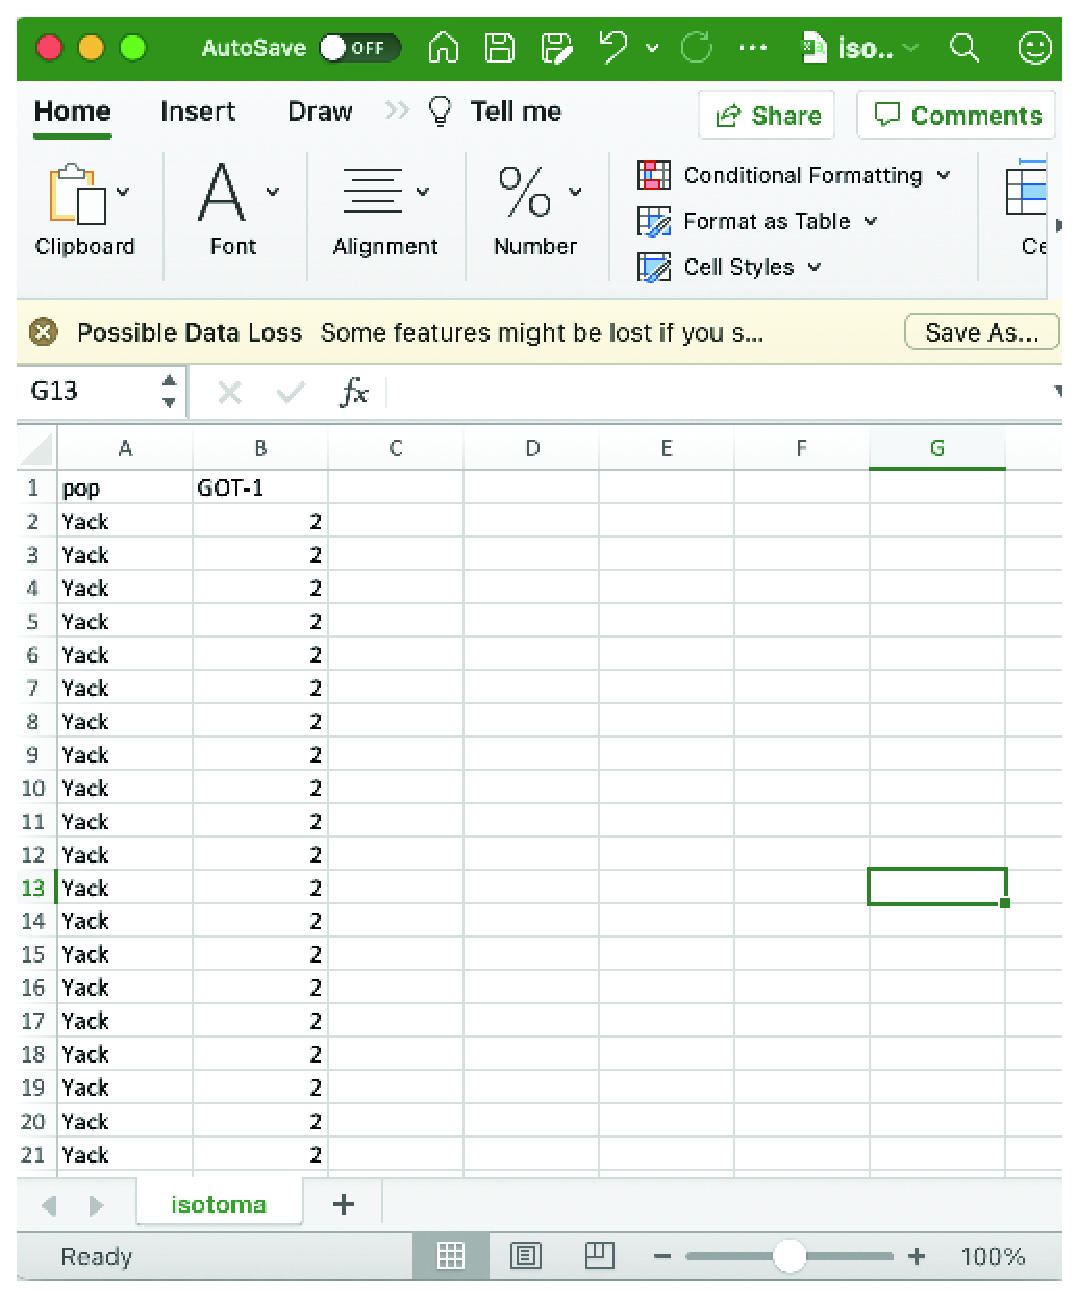
\includegraphics{isotoma-csv.eps}}
  \end{center}
\caption{Selected rows of a {\tt isotoma.csv} with data from {\it
    Isotoma petraea}~\cite{James-etal-1983}.}\label{fig:isotoma-csv}
\end{figure}

The first row is a header row that describes the data in the
columns. The first column has the heading {\tt pop}, which indicates
that the elements in the column refer to the population from which an
individual was collected. The second column has the heading {\tt
  GOT-1}, which indicates that this column contains the genotype of an
individual at the {\tt GOT-1} locus. Each row after the first is the
genotype of one individual. I used 2 for $A_1A_1$, 1 for $A_1A_2$, and
0 for $A_2A_2$. I could have swapped the numbers for the two
homozygotes, but the heterozygote must be given the genotype 1.

Now load {\tt Hickory} and the {\tt tidyverse} and take a quick look
at a more complicated data set before we continue with the {\it
  Isotoma petraea\/} example.

\begin{verbatim}
library("Hickory")
library("tidyverse")
dat <- read_csv(system.file("extdata", "protea_repens.csv", package = "Hickory"))
view(dat)
\end{verbatim}

\noindent Here you'll see the {\tt pop} column again and columns for
the genotype of individuals at 20 different
loci~(Figure~\ref{fig:repens-csv}). For now just notice how
every individual has been genotyped at a number of loci, and that
there are missing data (denoted by '.') for some combinations of
individuals and loci.

\begin{figure}
  \begin{center}
    \resizebox{!}{8cm}{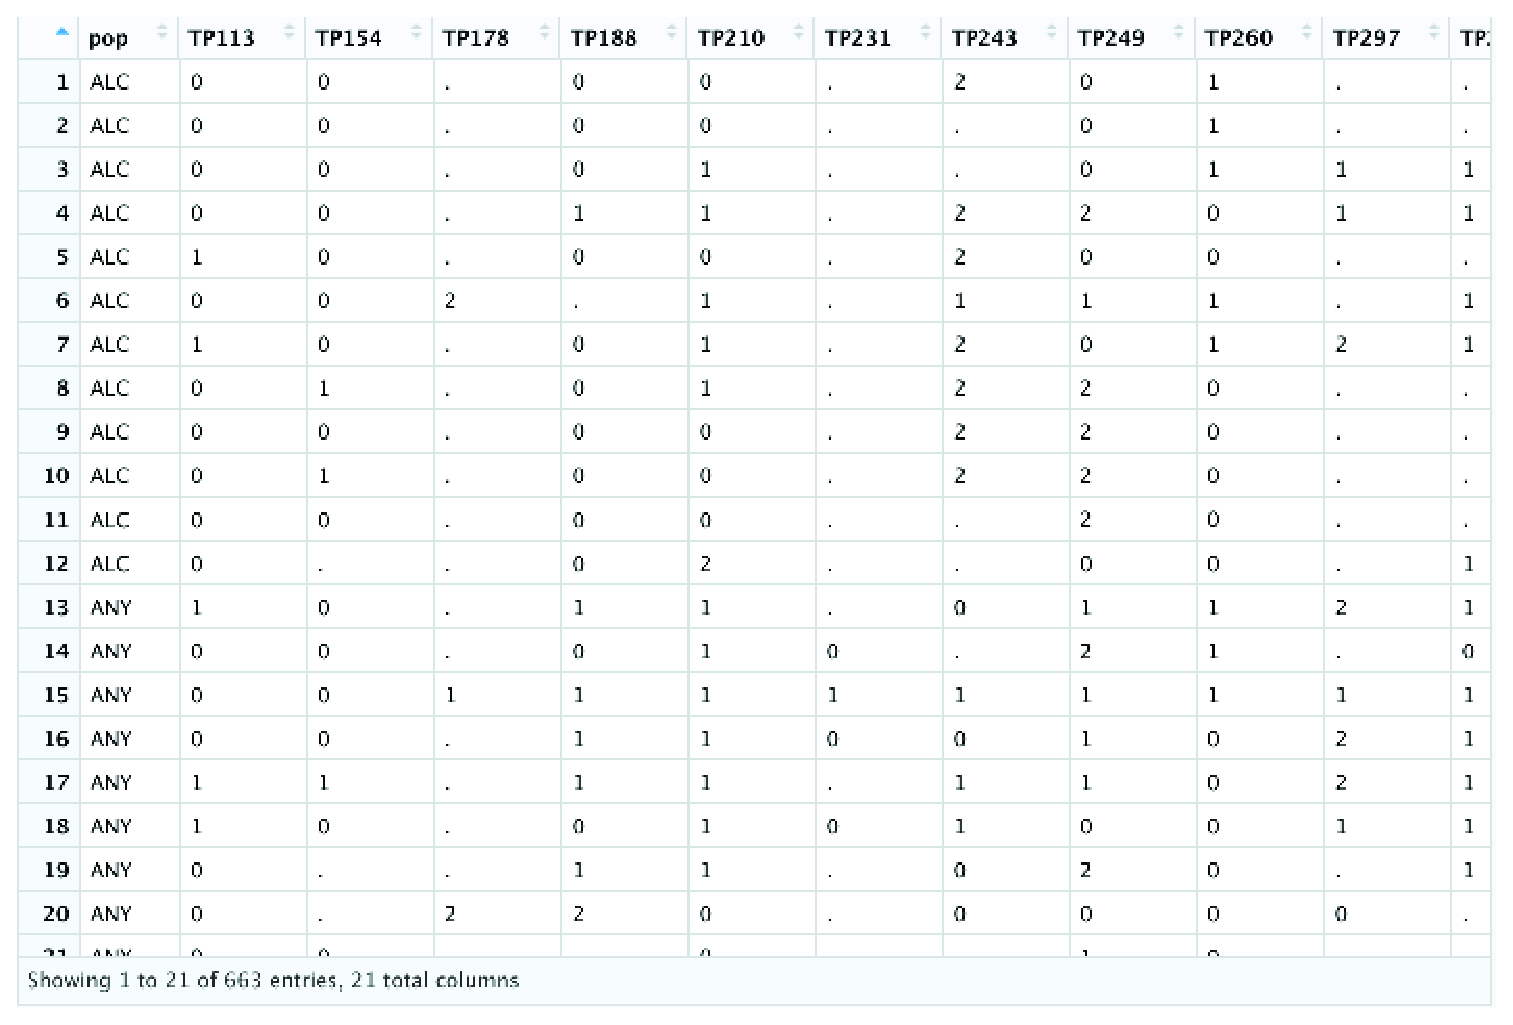
\includegraphics{repens-csv.eps}}
  \end{center}
\caption{Selected rows of a a data set from {\it Protea repens\/} that
  is distributed with {\tt Hickory}~\cite{Prunier-etal-2017}.}\label{fig:repens-csv}
\end{figure}

Now that you understand something about the format of the data that
{\tt Hickory} needs, let's load it into {\tt R} for further analysis.

\begin{verbatim}
genos <- read_marker_data("isotoma.csv")
\end{verbatim}

\subsubsection*{Running the analysis}

Now that the data are loaded, running the analysis is very
straightforward.

\begin{verbatim}
fit <- analyze_codominant(genos)
\end{verbatim}
The results are pretty easy to interpret, too.
{\small
\begin{verbatim}
Inference for Stan model: analyze_codominant.
4 chains, each with iter=2000; warmup=1000; thin=1; 
post-warmup draws per chain=1000, total post-warmup draws=4000.

          mean se_mean    sd     2.5%      25%      50%      75%    97.5% n_eff  Rhat
f        0.344   0.002 0.101    0.147    0.276    0.345    0.414    0.538  3539 1.000
theta    0.075   0.001 0.046    0.017    0.042    0.065    0.096    0.197  1223 1.002
lp__  -121.464   0.150 4.035 -130.283 -124.022 -121.095 -118.549 -114.516   727 1.003

Samples were drawn using NUTS(diag_e) at Sat Jul  3 16:07:48 2021.
For each parameter, n_eff is a crude measure of effective sample size,
and Rhat is the potential scale reduction factor on split chains (at 
convergence, Rhat=1).
\end{verbatim}
}
The column labeled {\tt mean} is the posterior mean for the parameter
listed in the first column.\footnote{Don't worry about {\tt lp\_\_}
for the time being.} The column labeled {\tt se\_mean} is the standard
error of the mean. It's a measure of how accurate the estimate of the
posterior mean is, and we want it to be very small relative to the
estimate of the posterior mean. The column labeled {\tt sd} is the
standard deviation of the posterior mean. It's a measure of our
uncertainty about the mean. We expect about 95\% of the posterior
probability to lie within 2 standard deviations of the mean. If we
compare the 2.5\% and 97.5\% quantiles,\footnote{Corresponding to 95\%
  of the posterior probabiity.} they are very close to what we expect.

In short, there appears to be a reasonable amount of inbreeding within
populations ($f = 0.344$) and a small to moderate amount of among
population differentiation ($\theta = 0.075$). In contrast to the Weir
and Cockerham method, we also have estimates of uncertainty associated
with both $f$ and $\theta$.\footnote{It's not too difficult to get
  estimates of uncertainty usins the Weir and Cockerham approach, but
  it takes some additional work.} Since you've probably forgotten what
the other estimates look like, Table~\ref{table:hickory-comparison}
compares all of the approaches we've considered.

\begin{table}
\begin{center}
  \begin{tabular}{c|ll}
\hline\hline
Method & $F_{is}$ & $F_{st}$ \\
\hline
Direct            & 0.137 & 0.214 \\
Nei               & 0.309 & 0.240 \\
Weir \& Cockerham & 0.540 & 0.039 \\
{\tt Hickory}     & 0.344 & 0.075 \\
\hline
\end{tabular}
\end{center}
\caption{Comparison of different approaches for estimating population
  structure from genetic data.}\label{table:hickory-comparison}
\end{table}

The logic behind {\tt Hickory\/} matches the logic behind Weir \&
Cockerham. With moderate to large sample sizes, the point estimates
are reasonably close. They're somewhat different here because there is
only one locus in the sample and because the sample sizes in some of
the populations are very small. Notice, however, that the {\tt
  Hickory} and the Weir \& Cockerham estimates are similar in one very
important respect. The estimate of $F_{ST}$ is much smaller in them
than in Nei's method or the direct method because they take account of
genetic sampling, not just statistical sampling.\index{genetic sampling}\index{statistical sampling}

\subsubsection*{Thinking about priors}

When I introduced the Bayesian model I reminded you that we need to
specify priors to complete it, so how did I get away without
specifying any priors in the analysis we just completed? Because {\tt
  Hickory} picks priors by default when you don't specify them. It
picks priors for $f$ and $\theta$ such that there's a 95\% chance that
they lie between 0.01 and 0.2. That makes sense for many organisms,
since many of them are outbreeding and have low to moderate amounts of
population differentiation. If we have a fair amount of data, that
choice won't make much difference. What about here?

Instead of starting our analysis thinking that we have a reasonably
good idea of what $f$ and $\theta$ ought to be, let's suppose we don't
have much of an idea at all. In particular, let's imagine that all
we're willing to say is that there's a 95\% chance that $f$ and
$\theta$ lie between 0.1 and 0.9. How do we incorporate that into the
analysis?

\begin{verbatim}
fit <- analyze_codominant(genos, prior_f = list(lower = 0.1, upper = 0.9), 
                          prior_theta = list(lower = 0.1, upper = 0.9))
\end{verbatim}
As you can see, the results are quite different from those we got
before.

{\small
\begin{verbatim}
Inference for Stan model: analyze_codominant.
4 chains, each with iter=2000; warmup=1000; thin=1; 
post-warmup draws per chain=1000, total post-warmup draws=4000.

          mean se_mean    sd     2.5%      25%      50%      75%    97.5% n_eff  Rhat
f        0.523   0.001 0.094    0.331    0.460    0.525    0.590    0.693  4027 0.999
theta    0.263   0.005 0.131    0.068    0.163    0.243    0.342    0.571   724 1.005
lp__  -122.391   0.184 4.255 -131.796 -125.070 -121.939 -119.311 -115.408   533 1.007

Samples were drawn using NUTS(diag_e) at Sat Jul  3 16:43:51 2021.
For each parameter, n_eff is a crude measure of effective sample size,
and Rhat is the potential scale reduction factor on split chains (at 
convergence, Rhat=1).
\end{verbatim}
}

The posterior mean of $f$ is now $0.523$ rather than $0.344$, and the
posterior mean of $\theta$ is now $0.263$ rather than $0.075$. If
you're following along, you're probably asking yourself ``Which of
those estimates should I believe?'' My advice is that you shouldn't
believe either of them very much. Remember what a Bayesian model looks
like.

$$
\mbox{P}(\phi|x) = \frac{\mbox{P}(x|\phi)\mbox{P}(\phi)}{\mbox{P}(x)}
$$

\noindent We get the posterior mean from the posterior distribution,
$\mbox{P}(\phi|x)$. If the posterior mean changes substantially based
on different choices for the prior, $\mbox{P}(\phi)$, it means that we
don't have enough data for the likelihood, $\mbox{P}(x|\phi)$ to
dominate the result. In simpler terms, if different choices for the
prior lead to markedly different conclusions, our confidence in those
conclusions depends heavily on our prior beliefs, not just the data
we've collected. Unless we have a lot of confidence in our prior
beliefs, we shouldn't have much confidence in the conclusions.

One of the nice things about a Bayesian approach is that it gives us a
straightforward way to assess how much to rely on inferences from the
data we've collected. If different priors have a large influence on
the posterior, as they do here, it tells us that the data we've
collected don't have much information about the parameters we're
interested in. If different priors don't have a large influence, then
the data {\it do\/} have a fair amount of information about the
parameters.\footnote{If it seems as if I'm repeating myself, I
  probably am, but I think this is a really immportant point that
  bears repeating.} 

There's a general lesson here: Think carefully about the prior
distribution on the parameters in {\it any\/} Bayesian model you use,
{\it and\/} consider exploring at least a couple of different choices
of priors to see if they have a large influence on your
conclusions. In addition, {\it pay attention to the credible
  intervals}. In both sets of analyses you've just seen, the credible
intervals are very wide. That in itself says that the data aren't
giving you a very clear idea of what the parameter is.

\subsection*{Assessing evidence for inbreeding and population
  differentiation}

You've already seen that {\tt Hickory} gives you estimates of the
credible intervals for $f$ and $\theta$, but if you're interested in
seeing whether there is evidence for inbreeding within populations or
for genetic differentiation among populations, you can't just look to
see whether the credible intervals overlap $0$. Why? because $f$ and
$\theta$ are defined to lie between 0 and 1 in {\tt Hickory} so they
can't overlap 0.\footnote{We noted a couple of lectures ago that $f$
  can be negative when it's understood as a measure of departure from
  Hardy-Weinber, but for computational reasons, {\tt Hickory}
  restricts it to $[0,1]$. If you're interested in the gory details of
  why, feel free to ask me.} In some data sets the posterior mean for
either or both may be substantially larger than 0, and the lower bound
of the credible interval may also be substantially larger than 0. In
such cases, you'd be pretty safe saying that you have evidence for
inbreeding or geographical differentiation, but what if you have a
situation like what you get from using the {\it Protea repens\/} data
set that is distributed with {\tt Hickory}.

{\small
\begin{verbatim}
genos <- read_marker_data(system.file("extdata", "protea_repens.csv", package = "Hickory"))
fit <- analyze_codominant(genos)

Inference for Stan model: analyze_codominant.
4 chains, each with iter=2000; warmup=1000; thin=1; 
post-warmup draws per chain=1000, total post-warmup draws=4000.

           mean se_mean     sd      2.5%       25%       50%       75%     97.5% n_eff  Rhat
f         0.005   0.000  0.002     0.002     0.003     0.005     0.006     0.010  5169 0.999
theta     0.081   0.000  0.008     0.066     0.075     0.081     0.086     0.097  1599 1.001
lp__  -6242.725   0.538 17.416 -6276.812 -6254.305 -6242.781 -6230.561 -6209.327  1048 1.005

Samples were drawn using NUTS(diag_e) at Sun Jul  4 12:52:05 2021.
For each parameter, n_eff is a crude measure of effective sample size,
and Rhat is the potential scale reduction factor on split chains (at 
convergence, Rhat=1).
\end{verbatim}
}

The posterior means and credible intervals in these data are
relatively insensitive to our choice of priors.\footnote{Don't take my
  word for it. Run the analysis yourself with the second set of priors
  we used above or with another set of priors that strikes your fancy
  and compare the results.} The posterior mean for $\theta$ is only
0.081, but the lower bound of the 95\% credible interval is 0.066 and
the credible interval is quite small, which gives us reasonably strong
evidence that $\theta > 0$, i.e., that there is genetic
differentiation among populations. But what about inbreeding within
populations? The posterior mean of $f$ is only 0.005, and the lower
bound of the 95\% credible interval is barely greater than 0, i.e.,
0.002. That doesn't seem like very good evidence either way, but can
we say something more?\footnote{Would I be asking this question if the
  answer were ``No''?}

We could simply do Hardy-Weinberg tests at every locus in every
population, but that could get pretty tedious. If we did that, we'd
also run into problemms with multiple tests, which inconvenient to
deal with. We'll take a different approach. Namely, we'll compare the
model we just fit with one that {\it assumes\/} there is no inbreeding
within populations, i.e., $f = 0$. The criterion we'll use to compare
the models is something known as the expected log predictive
density~\cite{Vehtari-etal-2017}. That's a mouthful, and the
mathematics is reasonably complicated, but it's easy enough to
interpret the results without understanding all of those details.

First, we run the model in which we assume $f = 0$ and store the
result in a different object.
\begin{verbatim}
fit_f0 <- analyze_codominant(genos, f_zero = TRUE)

Inference for Stan model: analyze_codominant.
4 chains, each with iter=2000; warmup=1000; thin=1; 
post-warmup draws per chain=1000, total post-warmup draws=4000.

           mean se_mean     sd      2.5%       25%       50%       75%     97.5% n_eff  Rhat
f         0.000     NaN  0.000     0.000     0.000     0.000     0.000     0.000   NaN   NaN
theta     0.081   0.000  0.008     0.067     0.076     0.080     0.086     0.097  1934 1.000
lp__  -6234.006   0.518 16.882 -6267.340 -6245.573 -6233.842 -6222.445 -6202.017  1060 1.001

Samples were drawn using NUTS(diag_e) at Sun Jul  4 13:21:39 2021.
For each parameter, n_eff is a crude measure of effective sample size,
and Rhat is the potential scale reduction factor on split chains (at 
convergence, Rhat=1).
\end{verbatim}
Notice that the estimate for $f$ is 0, as expected. Now we can
commpare the two models using {\tt loo()}.\footnote{I call the first
  object {\tt loo\_free} because in that model $f$ was free to vary.}
\begin{verbatim}
loo_free <- loo(fit)
loo_f0 <- loo(f0)
compare(loo_free, loo_f0)
\end{verbatim}
You'll see some warning messages when you run {\tt loo()} with these
data. In an ideal world, we'd do things a bit differently and get rid
of them, but in this case, we don't need to worry about them. Let's
focus on the table that was printed.
\begin{verbatim}
       elpd_diff se_diff
model2  0.0       0.0   
model1 -1.8       3.4   
\end{verbatim}
The column labeled {\tt elpd\_diff} is the difference in expected log
predictive density between the model with the highest elpd and the
model on the line in which the entry appears. The column labeled {\tt
  se\_diff} is the standard error of that difference. {\tt model 2}
refers to the second model named in the call to {\tt compare()}, i.e.,
the $f=0$ model ({\tt loo\_f0}), and {\tt model 1} refers to the first
model named in the call to {\tt compare()}, i.e., the $f$ ``free''
model. What all of this means is that

\begin{itemize}

  \item Model 2, the $f=0$ model, is more strongly supported than
    Model 2, the model in which we estimated $f$, {\it but}

  \item The difference between the two models, -1.8, is substantially
    less than twice the standard error of the difference (3.4),
    meaning that we don't have good evidence that one model is better
    than the other.
    
\end{itemize}

You may find it dissatisfying that we can't distinguish between these
two models and that we're left saying that we don't know whether we
have evidence for inbreeding within populations or not, but remember,
our estimate of $f$ is only
0.005. Table~\ref{table:f-model-comparison} shows what that means for
expected genotype frequencies if $p = 0.5$. As you can see, the
difference in genotype frequencies is extremely small. It's hard to
believe that there would be any biologically meaningful difference
between any of the scenarios that seem compatible with the data.

\begin{table}
  \begin{center}
    \begin{tabular}{l|lll}
      \hline\hline
      Model       & $A_1A_1$ & $A_1A_2$ & $A_2A_2$ \\
      \hline
      $f = 0$     & 0.25     & 0.50    & 0.25 \\
      $f = 0.005$ & 0.25125  & 0.4975  & 0.25125 \\
      $f = 0.010$ & 0.2525   & 0.495   & 0.2525 \\
      \hline
    \end{tabular}
  \end{center}
  \caption{Comparison of genotype frequencies assuming $p = 0.5$ with
    $f = 0$ and $f$ as estimated (mean and upper bound of the 95\%
    credible interval) from the {\it Protea repens\/} data distributed
    with {\tt Hickory}.}\label{table:f-model-comparison}
\end{table}

\bibliography{popgen}
\bibliographystyle{plain}

\ccLicense

\end{document}

\documentclass[12pt]{article}
\usepackage{lecture}
\usepackage{html}
\usepackage{graphics}
\usepackage{epstopdf}

\newcommand{\copyrightYears}{2004-2021}

\title{Analyzing the genetic structure of populations: individual assignment}

\begin{document}

\maketitle

\thispagestyle{first}

\section*{Introduction}

Although $F$-statistics are widely used and very informative, they
suffer from one fundamental limitation: We have to know what the
populations are before we can estimate them.\footnote{To be a little
  more precise~(and more than a little pedantic), we have to {\it
    assume\/} that the sample locations we decide to treat as
  populations are discrete, well-mixed populations that are distinct
  from others.} They are based on a conceptual model in which
organisms occur in discrete populations, populations that are both (1)
well mixed within themselves (so that we can regard our sample of
individuals as a random sample from within each population) and (2)
clearly distinct from others. What if we want to use the genetic data
itself to help us figure out what the populations actually are? Can we
do that?\footnote{Would I be asking this question if the answer were
  ``No?''}

A little over 20 years ago a different approach to the analysis of
genetic structure began to emerge: analysis of individual
assignment.\index{individual assignment} Although the implementation
details get a little hairy,\footnote{OK, to be fair. They get {\it
    very\/} hairy.} the basic idea is fairly simple. I'll give an
outline of the math in a moment, but let's do this in words
first. Suppose we have data on a series of individuals. If two
individuals are part of the same population, we expect them to be more
similar to one another than they are to individuals in other
populations. So if we ``cluster'' individuals that are ``genetically
similar'' to one another, those clusters should correspond to
populations. Rather than pre-defining the populations, we will have
allowed the data to tell us what the populations are. We haven't even
required {\it a priori\/} that individuals be grouped according to
their geographic proximity. Instead, we can examine the clusters we
find and see if they make any sense geographically.

Now for an outline of the math. Label the data we have for each
individual $x_i$. Suppose that all individuals belong to one of $K$
populations\footnote{Remember the peculiar thing I mentioned about
  population geneticists earlier? We like to imagine we know something
  even when we don't. In this case, I'm imagining we know that there
  are $K$ even though we don't. If we knew $K$, we'd probably already
  know which individual belonged in which population. We'll get to the
  problem of determining what $K$ is later.} and let the genotype
frequencies in population $k$ be represented by $\gamma_k$. Then the
likelihood that individual $i$ comes from population $k$ is just
\[
\mbox{P}(i|k) = \frac{\mbox{P}(x_i|\gamma_k)}{\sum_k
  \mbox{P}(x_i|\gamma_k)} \quad .
\]
So if we can specify prior probabilities for $\gamma_k$, we can use
Bayesian methods to estimate the posterior probability that individual
$i$ belongs to population $k$, and we can associate that assignment
with some measure of its reliability.\footnote{You can find details
  in~\cite{Pritchard-etal-2000}. If you think about that equation a
  bit, you can begin to see why the details get {\it very\/}
  hairy. First, we're trying to get the data to tell us what the
  populations are, so we don't even know how many populations there
  are. Then we have to find a way of estimating allele frequencies
  (and genotype frequencies) in populations when we don't even know
  which populations individuals in our sample belong in.}  Remember,
though, that we've arrived at the assignment by {\it assuming\/} that
there are $K$ populations. Since we don't know $K$, we have to find a
way of estimating it. Different choices of $K$ may lead to different
patterns of individual assignment, which complicates our
interpretation of the results.\footnote{This is an example of the ``no
  free lunch'' principle. You don't get something for nothing. Here we
  gained the ability to have the data tell us what the populations
  are, but we made interpreting the results more difficult.}

\section*{Applying assignment to understand invasions}

To see a simple example of how {\tt
  Structure}\index{Structure@\texttt{Structure}} can be used, we'll
use it to assess whether cultivated genotypes of {\it Berberis
  thunbergii\/}\index{Berberis@\textit{Berberis}!\textit{thunbergii}}
contribute to ongoing invasions in Connecticut and
Massachusetts~\cite{Lubell-etal-2008}.\index{individual assignment!application} The first problem is to determine what $K$
to use, because $K$ doesn't necessarily have to equal the number of
populations we sample from. Some populations may not be distinct from
one another. There are a couple of ways to estimate $K$. The most
straightforward is to run the analysis for a range of plausible
values, repeat it 10-20 times for each value, calculate the mean ``log
probability of the data'' for each value of $K$, and pick the value of
$K$ that is the biggest, i.e., the least
negative~(Table~\ref{table:berberis-k}). For the barberry data, $K=3$
is the obvious choice.\footnote{As part of her dissertation, Nora
  Mitchell used {\tt Structure} to study a hybrid zone between two
  species of {\it Protea}~\cite{Mitchell-Holsinger-2018}. Nora was
  interested in determining the extent to which individuals reflected
  ancestry from one of the two species involved. She set $K=2$ to
  separate individuals as cleanly into two categories as possible and
  used the individual assignment score as an index of hybridity. There
  wasn't any reason to attempt to infer $K$ from the data.}

\begin{table}
\begin{center}
\begin{tabular}{cc}
\hline\hline
K & Mean L(K) \\
\hline
2 & -2553.2 \\
3 & {\bf -2331.9} \\
4 & -2402.9 \\
5 & -2476.3 \\
\hline
\end{tabular}
\end{center}
\caption{Mean log probability of the data for $K=2,3,4,5$ in the {\it
    Berberis thunbergii\/} data~(adapted
  from~\cite{Lubell-etal-2008}).}\label{table:berberis-k}
\end{table}

Having determined that the data support $K=3$, the results of the
analysis are displayed in Figure~\ref{fig:lubell-structure}. Each
vertical bar corresponds to an individual in the sample, and the
proportion of each bar that is of a particular color tells us the
posterior probability that the individual belongs to the cluster with
that color.

\begin{figure}
\resizebox{\textwidth}{!}{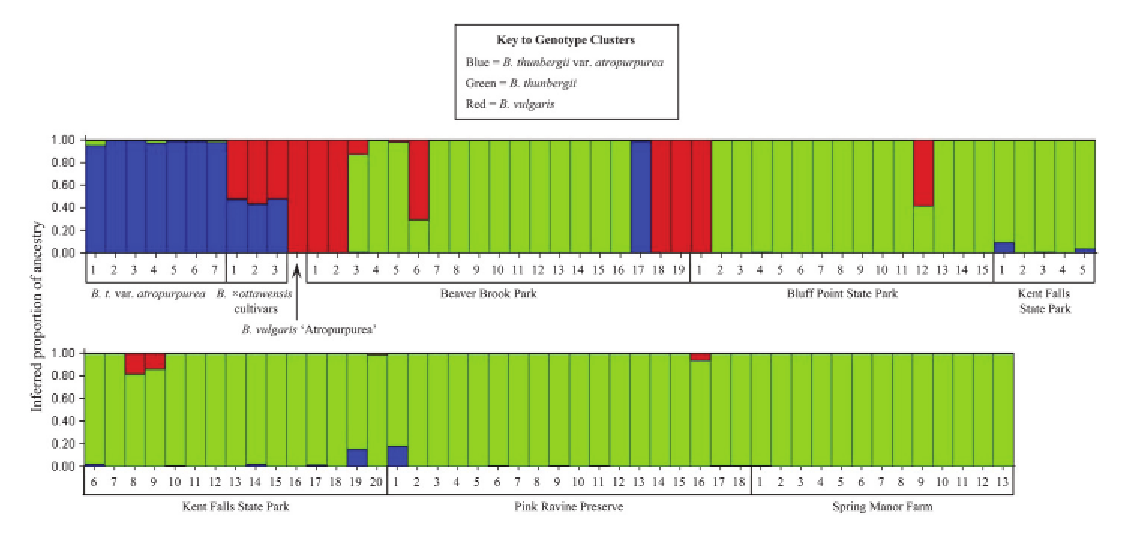
\includegraphics{lubell-structure.eps}}
\caption{Analysis of AFLP data from {\it Berberis
    thunbergii}~\cite{Lubell-etal-2008}.}\label{fig:lubell-structure} 
\end{figure}

Figure~\ref{fig:lubell-structure} may not look terribly informative,
but actually it is. Look at the labels beneath the figure. You'll see
that with the exception of individual 17 from Beaver Brook Park, all
the of the individuals that are solid blue are members of the
cultivated {\it Berberis thunbergii\/} var. {\it atropurpurea}. The
solid red bar corresponds to {\it Berberis vulgaris\/} 'Atropurpurea',
a different modern cultivar.\footnote{I find it very confusing that
  {\it Berberis thunbergii\/} var. {\it atropurpurea\/} and {\it
    Berberis vulgaris\/} 'Atropurpurea' both have ``atropurpurea''
  associated with their names, but that's the way life is.} You'll
notice that individuals 1, 2, 18, and 19 from Beaver Brook Park and
individual 1 from Bluff Point State Park fall into the same genotypic
cluster as this cultivar. {\it Berberis $\times$ottawensis} is a
hybrid cultivar whose parents are {\it Berberis thunbergii\/} and {\it
  Berberis vulgaris\/}, so it makes sense that individuals of this
cultivar would be half blue and half red. The solid green bars are
feral individuals from long-established populations. Notice that the
cultivars are distinct from all but a few of the individuals in the
long-established feral populations, suggesting that contemporary
cultivars are doing relatively little to maintain the invasion in
areas where it is already established.

\section*{Genetic diversity in human populations}\index{humans}

A much more interesting application of {\tt Structure} appeared a
shortly after {\tt Structure} was introduced. The Human Genome
Diversity Cell Line Panel (HGDP-CEPH)\index{HGDP-CEPH} consisted at
the time of data from 1056 individuals in 52 geographic
populations. Each individual was genotyped at 377 autosomal loci. If
those populations are grouped into 5 broad geographical
regions~(Africa, [Europe, the Middle East, and Central/South Asia],
East Asia, Oceania, and the Americas), we find that about 93\% of
genetic variation is found within local populations and only about 4\%
is a result of allele frequency differences between
regions~\cite{Rosenberg-etal-2002}. You might wonder why Europe, the
Middle East, and Central/South Asia were grouped together for that
analysis. The reason becomes clearer when you look at a {\tt
  Structure} analysis of the data~(Figure~\ref{fig:HGDP-CEPH}).

\begin{figure}
\resizebox{\textwidth}{!}{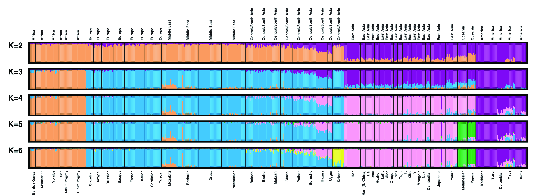
\includegraphics{HGDP-CEPH.eps}}
\caption{{\tt Structure} analysis of microsatellite diversity in the
  Human Genome Diversity Cell Line
  Panel~(from~\cite{Rosenberg-etal-2002}).}\label{fig:HGDP-CEPH} 
\end{figure}

\subsection*{A non-Bayesian look at individual-based analysis of
  genetic structure}

{\tt Structure} has a lot of nice features, but you'll discover a
couple of things about it if you begin to use it seriously: (1) It
often isn't obvious what the ``right'' {\tt K} is.\footnote{In fact,
  it's not clear that there {\it is\/} such a thing as the ``right''
  {\tt K}. If you're interested in hearing more about that. Feel free
  to ask.} (2) It requires a {\it lot\/} of computational resources,
especially with datasets that include a few thousand SNPs, as is
becoming increasingly common. An alternative is to use principal
component analysis directly on genotypes. There are technical details
associated with estimating the principal components and interpreting
them that we won't discuss,\footnote{See~\cite{Novembre-Stephens-2008}
  for details}, but the results can be pretty
striking. Figure~\ref{fig:human-PCA} shows the results of a PCA on
data derived from 3192 Europeans at 500,568 SNP loci. The
correspondence between the position of individuals in PCA space and
geographical space is remarkable. 

\begin{figure}
\resizebox{\textwidth}{!}{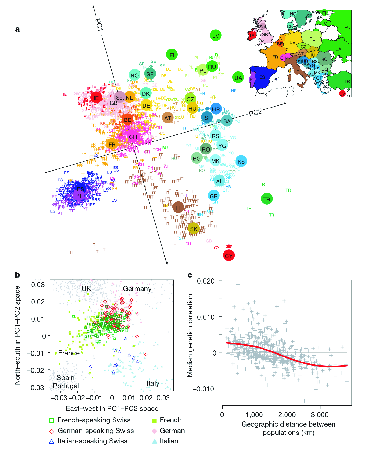
\includegraphics{human-PCA.eps}}
\caption{Principal components analysis of genetic diversity in Europe
  corresponds with
  geography~(from~\cite{Novembre-etal-2008}). Panel b is a close-up
  view of the area around Switzerland~(CH).}\label{fig:human-PCA}
\end{figure}

\section*{Other approaches}

Jombart et al.~\cite{Jombart-etal-2010} describe a related method
known as discriminant analysis of principal components. They also
provide an {\tt R} package, {\tt dapc}, that implements the
method.\index{Discriminant analysis of population structure} I prefer
{\tt Structure} because its approach to individual assignment is based
directly on population genetic principles, and since computers are
getting so fast~(especially when you have a computational cluster
available) that I worry less about how long it takes to run an
analysis on large datasets.\footnote{I also remember that a very long
  time ago when systematists were complaining that likelihood analyses
  of their data sets were taking a couple of weeks, Joe Felsenstein
  was reported to have said ``Why are you complaining that your
  analysis is taking a couple of weeks when you spent a couple of
  years collecting the data?''} That being said, Gopalan et
al.~\cite{Gopalan-etal-2016} released {\tt teraStructure} about five
years ago, which can analyze data sets consisting of 10,000
individuals scored at a million SNPs in less than 10
hours.\index{teraStructure@\texttt{teraStructure}} I haven't tried it
myself, because I haven't had a large data set to try it on, but you
should keep it in mind if you collect SNP data on a large number of
loci. Here are a couple more alternatives to consider that I haven't
investigated yet:

\begin{itemize}

\item {\tt sNMF} estimates individual admixture coefficients. It is
  reportedly 10-30 faster than the likelihood based {\tt ADMIXTURE},
  which is itself faster than {\tt Structure}. {\tt sNMF} is part of
  the {\tt R} package {\tt LEA}.

\item Meisner and Albrecthsen~\cite{Meisner-Albrechtsen-2018} present
  both a principal components method and an admixture method that
  accounts for sequencing errors inherent in low-coverage next
  generation DNA sequencing data.

\end{itemize}

\bibliography{popgen}
\bibliographystyle{plain}

\ccLicense

\end{document}


\part{The genetics of natural selection}

\documentclass[12pt]{article}
\usepackage{lecture}
\usepackage{html}
\usepackage{url}
\usepackage{graphics}
\usepackage{epstopdf}

\newcommand{\copyrightYears}{2001-2021}

\title{The Genetics of Natural Selection}

\begin{document}

\maketitle

\thispagestyle{first}

\section*{Introduction}

So far in this course, we've focused on describing the pattern of
variation within and among populations. We've talked about inbreeding,
which causes {\it genotype\/} frequencies to change, although it
leaves allele frequencies the same, and we've talked about how to
describe variation among populations. But we haven't yet discussed any
evolutionary processes that could lead to a change in allele
frequencies within populations.\footnote{We mentioned migration and
  drift in passing, and I'm sure you all understand the rudiments of
  them, but we haven't yet discussed them in detail.}

Let's return for a moment to the list of assumptions we developed when
we derived the Hardy-Weinberg principle and see what we've done so
far.

\begin{description}

\item[Assumption \#1] Genotype frequencies are the same in males and
females, e.g., $x_{11}$ is the frequency of the $A_1A_1$ genotype in
both males and females.

\item[Assumption \#2] Genotypes mate at random {\it with respect to
their genotype at this particular locus}.

\item[Assumption \#3] Meiosis is fair. More specifically, we assume
that there is no segregation distortion, no gamete competition, no
differences in the developmental ability of eggs, or the fertilization
ability of sperm.

\item[Assumption \#4] There is no input of new genetic material, i.e.,
gametes are produced without mutation, and all offspring are produced
from the union of gametes within this population.

\item[Assumption \#5] The population is of infinite size so that the
actual frequency of matings is equal to their expected frequency and
the actual frequency of offspring from each mating is equal to the
Mendelian expectations.

\item[Assumption \#6] All matings produce the same number of
offspring, on average.

\item[Assumption \#7] Generations do not overlap.

\item[Assumption \#8] There are no differences among genotypes in the
probability of survival.

\end{description}

The only assumption we've violated so far is Assumption \#2, the
random-mating assumption. We're going to spend the next several
lectures talking about what happens when you violate Assumption \#3,
\#6, or \#8. When any one of those assumptions is violated we have
some form of natural selection going on.\footnote{As I alluded to when
  we first started talking about inbreeding, we can also have natural
  selection as a result of certain types of violations of assumption
  \#2, e.g., sexual selection or disassortative mating. See
  below.}\index{natural selection}

\subsection*{Components of selection}

Depending on which of those three assumptions is violated and how it's
violated we recognize that selection may happen in different ways and
at different life-cycle stages.\footnote{To keep things {\it
    relatively\/} simple we're not even going to discuss differences
  in fitness that may be associated with different ages. We'll assume
  a really simple life-cycle in which there are non-overlapping
  generations. So we don't need to distinguish between fitness
  components that differ among age categories.}\index{components of
  selection}\index{natural selection!components of selection}

\begin{description}

\item[Assumption \#3:] {\it Meiosis is fair}. There are at least two
  ways in which this assumption may be violated.

\begin{itemize}

\item {\it Segregation distortion\/}: The two alleles are not equally
  frequent in gametes produced by heterozygotes. The $t$-allele in
  house mice, for example, is found in 95\% of fertile sperm produced
  by heterozygous males.\index{segregation distortion}\index{natural selection!segregation distortion}

\item {\it Gamete competition\/}: Gametes may be produced in equal
  frequency in heterozygotes, but there may be competition among them
  to produce fertilized zygotes, e.g., sperm competition in animals,
  pollen competition in seed plants.\index{gamete
    competition}\index{natural selection!gamete competition}\footnote{Strictly speaking pollen competition isn't
    gamete competition, although the evolutionary dynamics are the
    same. I'll leave it to the botanists among you to explain to the
    zoologists why pollen competition would be more properly called
    {\it gametophytic\/} competition.}

\end{itemize}

\item[Assumption \#6:] {\it All matings produce the same number of
progeny.}

\begin{itemize}

\item {\it Fertility selection\/}: The number of offspring produced
  may depend on maternal genotype ({\it fecundity selection\/}),
  paternal genotype ({\it virility selection\/}), or on
  both.\index{fertility selection}\index{fecundity selection}\index{virility selection}\index{natural selection!fertility selection}

\end{itemize}

\item[Assumption \#8:] {\it Survival does not depend on genotype.}

\begin{itemize}

\item {\it Viability selection\/}: The probability of survival from
  zygote to adult may depend on genotype, and it may differ between
  sexes.\index{viability selection}\index{natural selection!viability
    selection}

\end{itemize}

\end{description}

At this point you're probably thinking that I've covered all the
possibilities. But by now you should also know me well enough to guess
from the way I wrote that last sentence that if that's what you were
thinking, you'd be wrong. There's one more way in which selection can
happen that corresponds to violating

\begin{description}

\item[Asssumption \#2:] {\it Individuals mate at random.}

\begin{itemize}

\item {\it Sexual selection\/}: Some individuals may be more
  successful at finding mates than others. Since females are typically
  the limiting sex (Bateman's principle), the differences typically
  arise either as a result of {\it male-male competition\/} or {\it
    female choice}.\index{sexual selection}\index{natural selection!sexual selection}

\item {\it Disassortative mating\/}: When individuals preferentially
  choose mates different from themselves, rare genotypes are favored
  relative to common genotypes. This leads to a form a
  frequency-dependent selection.\index{disassortative mating}\index{natural selection!disassortative mating}

\end{itemize}

\end{description}

\section*{The genetics of viability selection}

That's a pretty exhaustive (and exhausting) list of the ways in which
selection can happen. We could spend the entire semester exploring
each of those. Instead, we're going to focus on viability
selection, but it's important to remember that any or all of the other
forms of selection may be operating simultaneously on the genes or the
traits that we're studying, and the direction of selection due to
these other components may be the same or different from the direction
of viability selection.

We're going to focus on viability selection for two reasons:\index{viability selection!genetics}

\begin{enumerate}

\item The most basic properties of natural selection acting on other
  components of the life history are similar to those of viability
  selection. A good understanding of viability selection provides a
  solid foundation for understanding other types of
  selection.\footnote{There are some important differences, however,
    and I hope we have time to discuss a couple of them.}

\item The algebra associated with understanding viability selection is
  a {\it lot\/} simpler than the algebra associated with understanding
  any other type of selection, and the dynamics are simpler and
  easier to understand.\footnote{Once you've seen what you're in for,
    you may think I've lied about this. But if you really think I
    have, just ask me to illustrate some of the algebra necessary for
    understanding viability selection when males and females differ in
    fitness. That's about as simple an extension as you can imagine,
    and things start to get pretty complicated even then.}

\end{enumerate}

\subsection*{The basic framework}

To understand the basics, we'll start with a numerical example using
some data on {\it Drosophila pseudoobscura\/} that Theodosius
Dobzhansky collected more than 70 years ago. You may remember that
this species has chromosome inversion polymorphisms. Although these
inversions involve many genes, they are inherited as if they were
single Mendelian loci, so we can treat the karyotypes as single-locus
genotypes and study their evolutionary dynamics. We'll be considering
two inversion types: the Standard inversion type, $ST$, and the
Chiricahua inversion type, $CH$. We'll use the following notation
throughout our discussion:\index{Drosophila@\textit{Drosophila}!\textit{pseudoobscura}}

\begin{center}
\begin{tabular}{cc}
\hline\hline
Symbol  & Definition \\
\hline
$N$      & number of individuals in the population \\
$x_{11}$ & frequency of $ST/ST$ genotype \\
$x_{12}$ & frequency of $ST/CH$ genotype \\
$x_{22}$ & frequency of $CH/CH$ genotype \\
$w_{11}$ & fitness of $ST/ST$ genotype, probability of surviving from
           egg to adult \\
$w_{12}$ & fitness of $ST/CH$ genotype \\
$w_{22}$ & fitness of $CH/CH$ genotype \\
\hline
\end{tabular}
\end{center}

The data look like this:\footnote{Don't worry for the moment about how
the viabilities were estimated.}

\begin{center}
\begin{tabular}{l|ccc}
\hline\hline
Genotype         & $ST/ST$    & $ST/CH$    & $CH/CH$    \\
\hline
Number in eggs   & 41       & 82       & 27       \\
                 & $x_{11}N$  & $x_{12}N$  & $x_{22}N$  \\
viability        & 0.6      & 0.9      & 0.45     \\
                 & $w_{11}$   & $w_{12}$   & $w_{22}$   \\
Number in adults & 25       & 74       & 12       \\
                 & $w_{11}x_{11}N$ & $w_{12}x_{12}N$ & $w_{22}x_{22}N$ \\
\hline
\end{tabular}
\end{center}

\section*{Genotype and allele frequencies}

It should be easy for you by this time to calculate the genotype
frequencies in eggs and adults.\footnote{At least it should be easy
  for you to calculate the frequencies using the numbers. It may not
  be so easy to do it with the symbols.} I'll refer to genotype
frequencies in eggs (or newly-formed zygotes) as genotype frequencies
{\it before selection\/} and genotype frequencies in adults as
genotype frequencies {\it after selection}.

\begin{eqnarray*}
\mbox{freq($ST/ST$) before selection}
 &=& \frac{41}{41 + 82 + 27} \\
 &=& 0.27 \\
\mbox{freq($ST/ST$) before selection}
 &=& \frac{Nx_{11}}{Nx_{11} + Nx_{12} + Nx_{22}} \\
 &=& x_{11} \\
 && \\
\mbox{freq($ST/ST$) after selection}
 &=& \frac{25}{25 + 74 +12} \\
 &=& 0.23 \\
\mbox{freq($ST/ST$) after selection}
 &=& \frac{w_{11}x_{11}N}{w_{11}x_{11}N + w_{12}x_{12}N + w_{22}x_{22}N} \\
 &=& \frac{w_{11}x_{11}}{w_{11}x_{11} + w_{12}x_{12} +
 w_{22}x_{22}} \\
 &=& \frac{w_{11}x_{11}}{\bar w} \\
 \bar w &=& \frac{w_{11}x_{11}N + w_{12}x_{12}N + w_{22}x_{22}N}{N} \\
        &=& w_{11}x_{11} + w_{12}x_{12} + w_{22}x_{22} \quad .
\end{eqnarray*}
$\bar w$ is the mean fitness, i.e., the average probability of
survival in the population.\index{mean fitness}

If you followed that, you shouldn't have much trouble following how to
calculate the allele frequencies before and after selection:

\begin{eqnarray*}
\hbox{freq($ST$) before selection}
 &=& \frac{2(41) + 82}{2(41 + 82 + 27)} \\
 &=& 0.55 \\
\hbox{freq($ST$) before selection}
 &=& \frac{2(Nx_{11}) + Nx_{12}}{2(Nx_{11} + Nx_{12} + Nx_{22})} \\
 &=& x_{11} + x_{12}/2 \\
&& \\
\hbox{freq($ST$) after selection}
 &=& \frac{2(25) + 74}{2(25 + 74 + 12)} \\
 &=& 0.56 \\
\hbox{freq($ST$) after selection}
 &=& \frac{2w_{11}x_{11}N + w_{12}x_{12}N}{2(w_{11}x_{11}N + w_{12}x_{12}N + w_{22}x_{22}N)} \\
 &=& \frac{2w_{11}x_{11} + w_{12}x_{12}}{2(w_{11}x_{11} + w_{12}x_{12} + w_{22}x_{22})} \\
p' &=& \frac{w_{11}x_{11} + w_{12}x_{12}/2}{w_{11}x_{11} +
 w_{12}x_{12} + w_{22}x_{22}} \\
x_{11} &=& p^2, \quad x_{12} = 2pq, \quad x_{22} = q^2 \\
p' &=& \frac{w_{11}p^2 + w_{12}pq}{w_{11}p^2 + w_{12}2pq + w_{22}q^2} \\
\bar w &=& w_{11}x_{11} + w_{12}x_{12} + w_{22}x_{22} \\
       &=& p^2w_{11} + 2pqw_{12} + q^2w_{22}
\end{eqnarray*}

If you're still awake, you're probably wondering\footnote{Okay,
  ``probably'' is an overstatement. ``May be'' would have been a
  better guess.} why I was able to substitute $p^2$, $2pq$, and $q^2$
for $x_{11}$, $x_{12}$, and $x_{22}$. Remember what I said earlier
about what we're doing here. The {\it only\/} Hardy-Weinberg
assumption we're violating is the one saying that all genotypes are
equally likely to survive from zygote to adult. Remember also that a
single generation in which all of the conditions for Hardy-Weinberg is
enough to establish the Hardy-Weinberg proportions. Putting those two
observations together, it's not too hard to see that genotypes will be
in Hardy-Weinberg proportions in newly formed zygotes. Viability
selection will change the genotype frequencies later in the
life-cycle, but we restart every generation with {\it zygotes\/} in
the familiar Hardy-Weinberg proportions, $p^2$, $2pq$, and $q^2$,
where $p$ is the frequency of $ST$ in the {\it parents\/} of those
zygotes.\index{selection equation} An important implication of this
that we'll return to later, is that we can understand the dynamics of
viability selection by focusing on how {\it allele\/} frequencies
change. One of the reasons that other forms of natural selection are
more complicated to understand is that we have to understand the
dynamics of genotype frequencies, meaning that instead of one
(relatively) simple equation we have at least two.

\subsection*{Selection acts on relative viability}

Let's stare at the selection equation for awhile and see what it
means.
\begin{equation}
p' = \frac{w_{11}p^2 + w_{12}pq}{\bar w} \quad . \label{eq:absolute}
\end{equation}
Suppose, for example, that we were to divide the numerator and
denominator of~(\ref{eq:absolute}) by $w_{11}$.\footnote{I'm dividing
  by 1, in case you hadn't noticed. When I'm not adding zero to an
  equation, I'm dividing by one. If you're not used to that yet, you
  will be in a few more weeks.} We'd then have
\begin{equation}
p' = \frac{p^2 + (w_{12}/w_{11})pq}{(\bar w/w_{11})} \quad . \label{eq:relative}
\end{equation}
Why did I bother to do that? Well, notice that we start with the same
allele frequency, $p$, in the parental generation in both equations
and that we end up with the same allele frequency in the offspring
generation, $p'$, in both equations, but the fitnesses are different:
\begin{center}
\begin{tabular}{c|ccc}
\hline\hline
         & \multicolumn{3}{c}{Fitnesses} \\
Equation & $A_1A_1$ & $A_1A_2$ & $A_2A_2$ \\
\hline
\ref{eq:absolute} & $w_{11}$ & $w_{12}$ & $w_{22}$ \\
\ref{eq:relative} & 1 & $w_{12}/w_{11}$ & $w_{22}/w_{11}$ \\
\hline
\end{tabular}
\end{center}
I could have, of course, divided the numerator and denominator by
$w_{12}$ or $w_{22}$ intead and ended up with yet other sets of
fitnesses that produce exactly the same change in allele
frequency. This illustrates the following general principle:
\begin{quote}
The consequences of natural selection (in an infinite population)
depend only on the {\it relative\/} magnitude of fitnesses, not on
their {\it absolute\/} magnitude.\index{relative fitness}
\end{quote}
That means, for example, that in order to predict the outcome of
viability selection, we don't have to know the probability that each
genotype will survive, i.e., their {\it absolute viabilities}. We only
need to know the probability that each genotype will survive relative
to the probability that other genotypes will survive, i.e., their {\it
  relative viabilities}. As we'll see later, it's sometimes easier to
estimate the relative viabilities than to estimate absolute
viabilities.\footnote{We'll also see when we get to studying the
  interaction between natural selection and drift that this statement
  is no longer true. To understand how drift and selection interact, we
  have to know something about {\it absolute\/}
  viabilities.}\index{viability!absolute}\index{viability!relative}

\subsection*{Marginal fitnesses}

In case you haven't already noticed, there's almost always more than
one way to write an equation.\footnote{And you won't have noticed this
  and may not believe me when I tell you, but I'm {\it not\/} showing
  you every possible way to write these equations.} They're all
mathematically equivalent, but they emphasize different things. In
this case, it can be instructive to look at the difference in allele
frequencies from one generation to the next, $\Delta p$:
\begin{eqnarray*}
\Delta p &=& p' - p \\
&=& \frac{w_{11}p^2 + w_{12}pq}{\bar w} - p \\
&=& \frac{w_{11}p^2 + w_{12}pq - \bar wp}{\bar w} \\
&=& \frac{p(w_{11}p + w_{12}q - \bar w)}{\bar w} \\
&=& \frac{p(w_1 - \bar w)}{\bar w} \quad ,
\end{eqnarray*}
where $w_1$ is the {\it marginal fitness\/} of allele $A_1$. To
explain why it's called a {\it marginal\/} fitness, I'd have to teach
you some probability theory that you probably don't want to
learn.\footnote{But remember this definition of marginal viability
anyway. You'll see it return in a few weeks when we talk about the
additive effect of an allele and about Fisher's Fundamental Theorem of
Natural Selection.} Fortunately, all you really need to know is that
it corresponds to the probability that a randomly chosen $A_1$ allele
in a newly formed zygote will survive into a reproductive
adult.\index{marginal fitness}

Why do we care? Because it provides some (relatively obvious)
intuition on how allele frequencies will change from one generation to
the next. If $w_1 > \bar w$, i.e., if the chances of a zygote carrying
an $A_1$ allele of surviving to make an adult are greater than the
chances of a randomly chosen zygote, then $A_1$ will increase in
frequency. If $w_1 < \bar w$, $A_1$ will decrease in frequency. Only
if $p=0$, $p=1$, or $w_1=\bar w$ will the allele frequency not change
from one generation to the next.

\section*{Patterns of natural selection}

Well, all that algebra was lots of fun,\footnote{Well, it was fun for
  me at least. Wasn't it fun for you, too?} but what good did it do
us? Not an enormous amount, except that it shows us~(not
surprisingly), that allele frequencies are likely to change as a
result of viability selection, and it gives us a nice little formula
we could plug into a computer to figure out exactly how. One of the
reasons that it's useful\footnote{If not exactly fun.} to go through
all of that algebra is that it's possible to make predictions about
the consequences of natural selection simply by knowing the pattern of
viaiblity differences. What do I mean by pattern? Funny you should
ask~(Table~\ref{table:patterns}).\index{natural selection!patterns}

\begin{table}
\begin{center}
\begin{tabular}{cc}
\hline\hline
Pattern & Description \\
\hline
Directional & $w_{11} > w_{12} > w_{22}$ \\
            & or \\
            & $w_{11} < w_{12} < w_{22}$ \\
Disruptive  & $w_{11} > w_{12}$, $w_{22} > w_{12}$ \\
Stabiliizing& $w_{11} < w_{12}$, $w_{22} < w_{12}$ \\
\hline
\end{tabular}
\end{center}
\caption{Patterns of viability selection at one locus with two alleles.}\label{table:patterns}
\end{table}

Before exploring the consequences of these different patterns of
natural selection, I need to introduce you to a very important result:
Fisher's Fundamental Theorem of Natural Selection. We'll go through
the details later when we get to quantitative genetics. In fact, we'll
derive Fisher's Fundamental Theorem for one locus and two alleles. For
now all you need to know is that viability selection causes the mean
fitness of the progeny generation to be greater than or equal to the
mean fitness of the parental generation, with equality only at
equilibrium, i.e.,
\[
\bar w' \ge \bar w \quad .
\]
How does this help us? Well, the best way to understand that is to
illustrate how we can use Fisher's theorem to predict the outcome of
natural selection when we know only the pattern of viability
differences. Let's take each pattern in turn.\index{Fisher's Fundamental Theorem of Natural Selection}

\subsection*{Directional selection}

To use the Fundamental Theorem we plot $\bar w$ as a function of
$p$~(Figure~\ref{fig:wbar}(a) and~\ref{fig:wbar}(b)). The Fundamental
Theorem now tells us that allele frequencies have to change from one
generation to the next in such a way that $\bar w' > \bar w$, which
can only happen if $p' > p$. So viability selection will cause the
frequency of the $A_1$ allele to increase in panel (a) and decrease in
panel (b).\index{directional selection}\index{selection!directional
  selection} Ultimately, the population will be monomorphic for the
homozygous genotype with the highest fitness.\footnote{A population is
  {\it monomorphic\/} at a particular locus when only one allele is
  present. If a population is monomorphic for allele $A_1$, I might
  also say that allele $A_1$ is fixed in the population or that the
  population is fixed for allele
  $A_1$.\index{monomorphic}\index{allele fixation}}

\begin{figure}
\begin{center}
\resizebox{!}{6in}{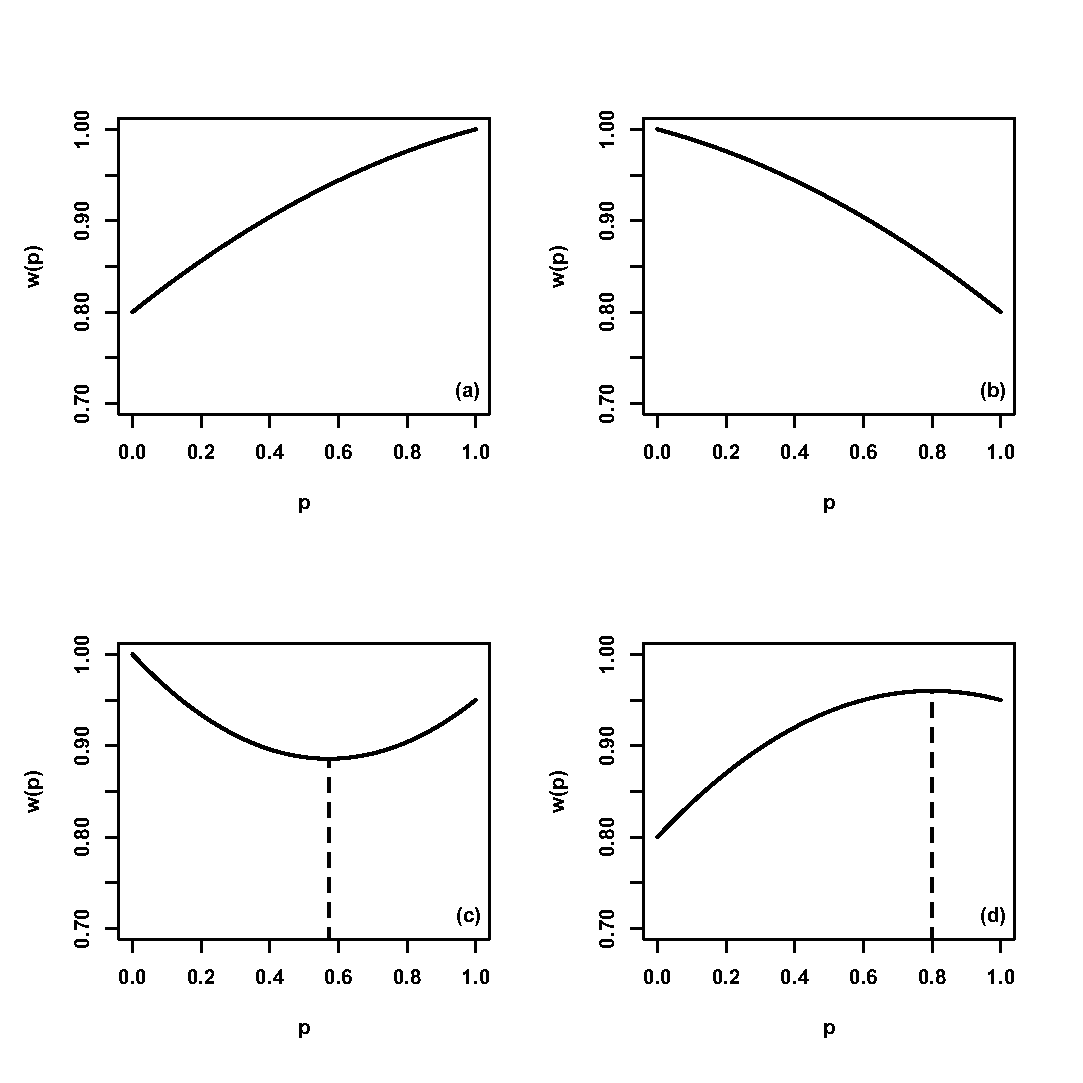
\includegraphics{wbar.eps}}
\end{center}
\caption{With {\it directional selection\/} (panel (a) $w_{11} > w_{12} >
w_{22}$, panel (b) $w_{11} > w_{12} > w_{22}$) viability selection
leads to an ever increasing frequency of
the favored allele.  Ultimately, the population will be monomorphic
for the homozygous genotype with the highest
fitness. With {\it disruptive selection\/} (panel (c) $w_{11} >
w_{12}$ and $w_{22} > w_{12}$) viability selection may lead either to
an increasing   frequency of the $A$ allele or to a decreasing frequency.
  Ultimately, the population will be monomorphic for one of the
  homozygous genotypes.  Which homozygous genotype comes to
  predominate, however, depends on the initial allele frequencies in
  the population. With {\it stabilizing selection\/} (panel (d) $w_{11} < w_{12}
  > w_{22}$; also called balancing selection or heterozygote
  advantage) viability selection will lead to a stable polymorphism.
  All three genotypes will be present at equilibrium.}\label{fig:wbar}
\end{figure}

\subsection*{Disruptive selection}

If we plot $\bar w$ as a function of $p$ when $w_{11} > w_{12}$ and
$w_{22} > w_{12}$, we see a very different
pattern~(Figure~\ref{fig:wbar}(c)). Since the Fundamental Theorem
tells us that $\bar w' \ge \bar w$, we know that if the population
starts with an allele on one side of the bowl $A_1$, will be lost. If
it starts on the other side of the bowl, $A_2$ will be
lost.\footnote{Strictly speaking, we need to know more than $\bar w'
  \ge \bar w$, but we do know the other things we need to know in this
  case. Trust me. Have I ever lied to you? (Don't answer
  that.)}\index{disruptive selection}\index{selection!disruptive}

Let's explore this example a little further. To do so, I'm going to
set $w_{11} = 1 + s_1$, $w_{12} = 1$, and $w_{22} = 1+
s_2$.\footnote{Why can I get away with this? Hint: Think about
  relative fitnesses.} When fitnesses are written this way $s_1$ and
$s_2$ are referred to as {\it selection coefficients}. Notice also
with these definitions that the fitnesses of the homozygotes are
greater than 1.\footnote{Which is why I gave you the relative fitness
  hint in the last footnote.} Using these definitions and plugging
them into~(\ref{eq:absolute}),\index{selection coefficient}
\begin{eqnarray}
p' &=& \frac{p^2(1+s_1) + pq}{p^2(1+s_1) + 2pq + q^2(1+s_2)} \nonumber
   \\
   &=& \frac{p(1 + s_1p)}{1 + p^2s_1 + q^2s_2} \quad . \label{eq:disruptive}
\end{eqnarray}
We can use equation~(\ref{eq:disruptive}) to find the equilibria of
this system, i.e., the values of $p$ such that $p' = p$.\index{equilibrium}
\begin{eqnarray*}
p &=& \frac{p(1 + s_1p)}{1 + p^2s_1 + q^2s_2} \\
p(1 + p^2s_1 + q^2s_2) &=& p(1 + s_1p) \\
p\left((1 + p^2s_1 + q^2s_2) - (1 + s_1p)\right) &=& 0 \\
p\left(ps_1(p - 1) + q^2s_2\right) &=& 0 \\
p(-pqs_1 + q^2s_2) &=& 0 \\
pq(-ps_q + qs_2) &=& 0 \quad .
\end{eqnarray*}
So the population is at equilibrium with $p'=p$ if $\hat p=0$,
$\hat q=0$, or $\hat ps_1 = \hat qs_2$.\footnote{Remember that the
  ``hats'' can mean either the estimate of an unknown paramter or an
  equilibrium. The context will normally make it clear which meaning
  applies. In this case it should be pretty obvious that I'm talking
  about equilibria.} We can simplify that last one a little further,
too.
\begin{eqnarray*}
\hat ps_1 &=& \hat qs_2 \\
\hat ps_1 &=& (1-\hat p)s_2 \\
\hat p(s_1 + s_2) &=& s_2 \\
\hat p &=& \frac{s_2}{s_1+s_2} \quad .
\end{eqnarray*}

Fisher's Fundamental Theorem tells us which of these equilibria
matter. I've already mentioned that depending on which side of the
bowl you start, you'll either lose the $A_1$ allele or the $A_2$
allele. But suppose you happen to start {\it exactly\/} at the bottom
of the bowl. That corresponds to the equilibrium with $\hat p =
s_2/(s_1+s_2)$. What happens then?

Well, if you start {\it exactly\/} there, you'll stay there forever
(in an infinite population). But if you start ever so slightly off the
equilibrium, you'll move farther and farther away. It's what
mathematicians call an {\it unstable equilibrium}. Any departure from
that equilibrium gets larger and larger. For evolutionary purposes, we
don't have to worry about a population getting to an unstable
equilibrium. It never will. Unstable equilibria are ones that
populations evolve away from.\index{equilibrium!unstable}

When a population has only one allele present it is said to be {\it
  fixed\/} for that allele. Since having only one allele is also an
equilibrium (in the absence of mutation), we can also call it a {\it
  monomorphic equilibrium}. When a population has more than one allele
present, it is said to be {\it polymorphic}. If two or more alleles
are present at an equilibrium, we can call it a {\it polymorphic
  equilibrium}. Thus, another way to describe the results of
disruptive selection is to say that the monomorphic equilibria are
stable, but that the polymorphic equilibrium is not.\footnote{Notice that a
  polymorphic equilibrium doesn't even exist when selection is
  directional.}\index{allele fixation}\index{equilibrium!monomorphic}\index{equilibrium!polymorphic}

\subsection*{Stabilizing selection}

If we plot $\bar w$ as a function of $p$ when $w_{11} < w_{12}$ and
$w_{22} < w_{12}$, we see a third pattern. The plot is shaped like an
upside down bowl~(Figure~\ref{fig:wbar}).\index{stabilizing selection}\index{selection!stabilizing}

In this case we can see that no matter what allele frequency the
population starts with, the only way that $\bar w' \ge \bar w$ can
hold is if the allele frequency changes in such a way that in every
generation it gets closer to the value where $\bar w$ is
maximized. Unlike directional selection or disruptive selection, in
which natural selection tends to eliminate one allele or the other,
stabilizing selection tends to keep both alleles in the
population. You'll also see this pattern of selection referred to as
balancing selection, because the selection on each allele is
``balanced'' at the polymorphic equilibria.\footnote{In fact, the
  marginal fitnesses are equal, i.e., $w_1=w_2$.} We can summarize the
results by saying that the monomorphic equilibria are unstable and
that the polymorphic equilibrium is stable. By the way, if we write
the fitness as $w_{11} = 1 - s_1$, $w_{12}=1$, and $w_{22}=1-s_2$,
then the allele frequency at the polymorphic equilibrium is $\hat
p=s_2/(s_1+s_2)$.\footnote{I'm not showing the algebra that justifies
  this conclusion on the off chance that you may want to test your
  understanding by verifying it yourself.} Notice that $\hat p$
depends only on the ratio of $s_1$ to $s_2$, not the magnitude. Again,
it is only {\it relative\/} fitnesses that matter.

\section*{Fertility selection}\index{natural selection!fertility selection}

So far we've been talking about natural selection that occurs as a
result of differences in the probability of survival, i.e., viability
selection. There are, of course, other ways in which natural selection
can occur:

\begin{itemize}

\item Heterozygotes may produce gametes in unequal frequencies, {\it
  segregation distortion}, or gametes may differ in their ability to
  participate in fertilization, {\it gametic selection}.\footnote{For
    the botanists in the room, I should point out that selection on
    the gametophyte stage of the life cycle (in plants with
    alternation of generations) is mathematically equivalent to
    gametic selection.}

\item Some genotypes may be more successful in finding mates than
  others, {\it sexual selection}.

\item The number of offspring produced by a mating may depend on
  maternal and paternal genotypes, {\it fertility selection}.

\end{itemize}

\noindent In fact, most studies that have measured components of
selection have identified far larger differences due to fertility than
to viability. Thus, fertility selection is a very important component
of natural selection in most populations of plants and animals. As
we'll see a little later, it turns out that sexual selection is
mathematically equivalent to a particular type of fertility
selection. But before we get to that, let's look carefully at the
mechanics of fertility selection.

\subsection*{Formulation of fertility selection}\index{natural selection!fertility selection, fertility matrix}

I introduced the idea of a fitness matrix earlier when we were
discussing selection at one locus with more than two alleles. Even if
we have only two alleles, it becomes useful to describe patterns of
fertility selection in terms of a fitness matrix. Describing the
matrix is easy. Writing it down gets messy. Each element in the table
is simply the average number of offspring produced by a given mated
pair. We write down the table with paternal genotypes in columns and
maternal genotypes in rows:
\begin{center}
\begin{tabular}{c|ccc}
\hline\hline
                  & \multicolumn{3}{c}{Paternal genotype} \\
Maternal genotype & $A_1A_1$ & $A_1A_2$ & $A_2A_2$ \\
\hline
$A_1A_1$ & $F_{11,11}$ & $F_{11,12}$ & $F_{11,22}$ \\
$A_1A_2$ & $F_{12,11}$ & $F_{12,12}$ & $F_{12,22}$ \\
$A_2A_2$ & $F_{22,11}$ & $F_{22,12}$ & $F_{22,22}$ \\
\hline
\end{tabular}
\end{center}
Then the frequency of genotype $A_1A_1$ after one generation of
fertility selection is:\footnote{I didn't say it, but you can probably
  guess that I'm assuming that all of the conditions for
  Hardy-Weinberg apply, except for the assumption that all matings
  leave the same number of offspring, on average.}
\begin{equation}
x_{11}' = \frac{x_{11}^2F_{11,11} + x_{11}x_{12}(F_{11,12} +
                F_{12,11})/2 + (x_{12}^2/4)F_{12,12}}{\bar F} \quad ,
\label{eq:fertility}
\end{equation}
where $\bar F$ is the mean fecundity of all matings in the
population.\footnote{As an exercise you might want to see if you can
derive the corresponding equations for $x_{12}'$ and $x_{22}'$.}

It probably won't surprise you to learn that it's very difficult to
say anything very general about how genotype frequenices will change
when there's fertility selection. Not only are there nine different
fitness parameters to worry about, but since genotypes are never
guaranteed to be in Hardy-Weinberg proportion, all of the algebra has
to be done on a system of three simultaneous equations.\footnote{And
you thought that dealing with one was bad enough!} There are three
weird properties that I'll mention:\index{natural selection!fertility selection, properties}

\begin{enumerate}

\item $\bar F'$ may be smaller than $\bar F$. Unlike selection on
viabilities in which fitness evolved to the maximum possible value,
there are situations in which fitness will evolve to the {\it
minimum\/} possible value when there's selection on
fertilities.\footnote{Fortunately, it takes rather weird fertility
schemes to produce such a result.}

\item A high fertility of heterozygote $\times$ heterozygote matings
is not sufficient to guarantee that the population will remain
polymorphic.

\item Selection may prevent loss of either allele, but there may be no
stable equilibria.

\end{enumerate}

\subsection*{Conditions for protected polymorphism}\index{natural selection!fertility selection, protected polymorphism}

There is one case in which it's fairly easy to understand the
consequences of selection, and that's when one of the two alleles is
very rare. Suppose, for example, that $A_1$ is very rare, then a
little algebraic trickery\footnote{The trickery isn't hard, just
tedious. Justifying the trickery is a little more involved, but not
too bad. If you're interested, drop by my office and I'll show you.}
shows that
\begin{eqnarray*}
x_{11}' &\approx& 0 \\
x_{12}' &\approx& \frac{x_{12}(F_{12,22} + F_{22,12})/2}{F_{22,22}}
\end{eqnarray*}
So $A_1$ will become more frequent if
\begin{equation}
(F_{12,22} + F_{22,12})/2 > F_{22,22} \label{eq:a-1}
\end{equation}
Similarly, $A_2$ will become more frequent when it's very rare when
\begin{equation}
(F_{11,12} + F_{12,11})/2 > F_{11,11} \label{eq:a-2} \quad .
\end{equation}
If both equation (\ref{eq:a-1}) and (\ref{eq:a-2}) are satisfied,
natural selection will tend to prevent either allele from being
eliminated. We have what's known as a {\it protected polymorphism}.

Conditions~(\ref{eq:a-1}) and~(\ref{eq:a-2}) are fairly easy to
interpret intuitively: There is a protected polymorphism if the
average fecundity of matings involving a heterozygote and the
``resident'' homozygote exceeds that of matings of the resident
homozygote with itself.\footnote{A ``resident'' homozygote is the one
  of which the populations is almost entirely composed when all but
  one allele is rare.}

{\bf NOTE:} It's entirely possible for neither inequality to be
satisfied {\it and\/} for their to be a stable polymorphism. In other
words, depending on where a population starts, selection may eliminate
one allele or the other or keep both segregating in the population in
a stable polymorphism.\footnote{Can you guess what pattern of
  fertilities is consistent with both a stable polymorphism and the
  {\it lack of\/} a protected polymorphism?}

\ccLicense

\end{document}

\documentclass[12pt]{article}
\usepackage{lecture}
\usepackage{html}
\usepackage{url}
\usepackage{graphics}
\usepackage{epstopdf}

\newcommand{\copyrightYears}{2001-2021}

\title{Estimating viability}

\begin{document}

\maketitle

\thispagestyle{first}

\section*{Introduction}

Being able to make predictions with known (or estimated) viabilities,
doesn't do us a heck of a lot of good unless we can figure out what
those viabilities are. Fortunately, figuring them out isn't too
hard.\footnote{I almost said that it was easy, but that would be going
  a bit too far.} If we know the number of individuals of each
genotype before selection, it's really easy as a matter of
fact.\footnote{And in the very next sentence I contradicted the last
  footnote. But it really is easy to estimate viabilities if we can
  genotype individuals before and after selection.} Consider that our
data looks like this:

\begin{center}
\begin{tabular}{l|ccc}
\hline\hline
Genotype & $A_1A_1$ & $A_1A_2$ & $A_2A_2$ \\
\hline
Number in zygotes & $n_{11}^{(z)}$ & $n_{12}^{(z)}$ & $n_{22}^{(z)}$ \\
Viability         & $w_{11}$ & $w_{12}$ & $w_{22}$ \\
Number in adults  & $n_{11}^{(a)} = w_{11}n_{11}^{(z)}$ & $n_{12}^{(a)} = w_{12}n_{12}^{(z)}$ & $n_{22}^{(a)} = w_{22}n_{22}^{(z)}$ \\
\hline
\end{tabular}
\end{center}

In other words, estimating the absolute viability simply consists of
estimating the probability that an individuals of each genotype that
survive from zygote to adult. The maximum-likelihood estimate is, of
course, just what you would probably guess:\index{viability!estimating absolute}
\[
w_{ij} = \frac{n_{ij}^{(a)}}{n_{ij}^{(z)}} \quad ,
\]
Since $w_{ij}$ is a probability and the outcome is binary (survive or
die), you should be able to guess what kind of likelihood relates the
observed data to the unseen parameter, namely, a binomial
likelihood. In {\tt Stan} notation:\footnote{You knew you were going
  to see this again, didn't you?}
\begin{verbatim}
   n_11_adult ~ binomial(n_11_zygote, w_11)
   n_12_adult ~ binomial(n_12_zygote, w_12)
   n_22_adult ~ binomial(n_22_zygote, w_22)
\end{verbatim}

\section*{Estimating relative viability}

To estimate absolute viabilities, we have to be able to identify
genotypes non-destructively, because we have to know what their
genotype was both {\it before\/} the selection event and {\it after\/}
the selection event. That's fine if we happen to be dealing with an
experimental situation where we can do controlled crosses to establish
known genotypes or if we happen to be studying an organism and a trait
where we can identify the genotype from the phenotype of a zygote (or
at least a very young individual) and from surviving
adults.\footnote{How many organisms and traits can you think of that
  satisfy this criterion? Any? There is one other possibility: If we
  can identify an individual's genotype after it's dead {\it and\/} if
  we can construct a random sample that includes both living and dead
  individuals {\it and\/} if we assume the probability of including an
  individual in the sample doesn't depend on whether that individual
  is dead or alive, then we can sample a population after the
  selection event and score genotypes both before and after the event
  from one set of observations.} What do we do when we can't follow
the survival of individuals with known genotype? Give
up?\footnote{Would I be asking the question if the answer were
  ``Yes''?}\index{viability!estimating relative}

Remember that to make inferences about how selection will act, we only
need to know {\it relative\/} viabilities, not {\it absolute\/}
viabilities.\footnote{At least that's true until we start worrying
  about how selection and drift interact.} We still need to know
something about the genotypic composition of the population before
selection, but it turns out that if we're only interested in relative
viabilities, we don't need to follow individuals. All we need to be
able to do is to score genotypes and estimate genotype frequencies
before and after selection. Our data looks like this:
\begin{center}
\begin{tabular}{l|ccc}
\hline\hline
Genotype & $A_1A_1$ & $A_1A_2$ & $A_2A_2$ \\
\hline
Frequency in zygotes & $x_{11}^{(z)}$ & $x_{12}^{(z)}$ &
$x_{22}^{(z)}$ \\
Frequency in adults  & $x_{11}^{(a)}$ & $x_{12}^{(a)}$ &
$x_{22}^{(a)}$ \\
\hline
\end{tabular}
\end{center}
We also know that
\begin{eqnarray*}
x_{11}^{(a)} &=& w_{11}x_{11}^{(z)}/\bar w \\
x_{12}^{(a)} &=& w_{12}x_{12}^{(z)}/\bar w \\
x_{22}^{(a)} &=& w_{22}x_{22}^{(z)}/\bar w \quad .
\end{eqnarray*}
Suppose we now divide all three equations by the middle one:
\begin{eqnarray*}
x_{11}^{(a)}/x_{12}^{(a)} &=& w_{11}x_{11}^{(z)}/w_{12}x_{12}^{(z)} \\
1 &=& 1 \\
x_{22}^{(a)}/x_{12}^{(a)} &=& w_{22}x_{22}^{(z)}/w_{12}x_{12}^{(z)} \quad ,
\end{eqnarray*}
or, rearranging a bit
\begin{eqnarray}
\frac{w_{11}}{w_{12}} &=& \left(\frac{x_{11}^{(a)}}{x_{12}^{(a)}}\right)
                          \left(\frac{x_{12}^{(z)}}{x_{11}^{(z)}}\right) 
\label{eq:est-rel-viability-1}
\\
\frac{w_{22}}{w_{12}} &=& \left(\frac{x_{22}^{(a)}}{x_{12}^{(a)}}\right)
                          \left(\frac{x_{12}^{(z)}}{x_{22}^{(z)}}\right)
\quad . \label{eq:est-rel-viability-2}
\end{eqnarray}
This gives us a complete set of relative viabilities.
\begin{center}
\begin{tabular}{l|ccc}
\hline\hline
Genotype & $A_1A_1$ & $A_1A_2$ & $A_2A_2$ \\
\hline
\\
Relative viability & $\frac{w_{11}}{w_{12}}$ & 1 &
$\frac{w_{22}}{w_{12}}$ \\
\\
\hline
\end{tabular}
\end{center}

If we use the maximum-likelihood estimates for genotype frequencies
before and after selection, we obtain maximum likelihood estimates for
the relative viabilities.\footnote{If anyone cares, it's because of
  the invariance property of maximum-likelihod estimates. If you don't
  understand what that is, don't worry about it, just trust me. Or if
  you want to know what the invariance principle is, ask.} If we
use Bayesian methods to estimate genotype frequencies before and after
selection (including the uncertainty around those estimates), we can
use these formulas to get Bayesian estimates of the relative
viabilities (and the uncertainty around them).

\section*{An example}\index{viability!example of estimating}

Let's see how this works with some real data from Dobzhansky's work on
chromosome inversion polymorphisms in {\it Drosophila
pseudoobscura.}\footnote{Taken from~\cite{Dobzhansky-1947}.}

\begin{center}
\begin{tabular}{l|ccc|c}
\hline\hline
Genotype & $ST/ST$ & $ST/CH$ & $CH/CH$ & Total \\
\hline
Number in larvae & 41 & 82 & 27 & 150 \\
Number in adults & 57 & 169 & 29 & 255 \\
\hline
\end{tabular}
\end{center}

You may be wondering how the sample of adults can be larger than the
sample of larvae. That's because to score an individual's inversion
type, Dobzhansky had to kill it. The numbers in larvae are based on a
sample of the population, and the adults that survived were not
genotyped as larvae. As a result, all we can do is to estimate the
relative viabilities.
\begin{eqnarray*}
\frac{w_{11}}{w_{12}} &=& \left(\frac{x_{11}^{(a)}}{x_{12}^{(a)}}\right)
                          \left(\frac{x_{12}^{(z)}}{x_{11}^{(z)}}\right)
= \left(\frac{57/255}{169/255}\right)
  \left(\frac{82/150}{41/150}\right)
= 0.67 \\
\frac{w_{22}}{w_{12}} &=& \left(\frac{x_{22}^{(a)}}{x_{12}^{(a)}}\right)
                          \left(\frac{x_{12}^{(z)}}{x_{22}^{(z)}}\right)
= \left(\frac{29/255}{169/255}\right)
  \left(\frac{82/150}{27/150}\right)
= 0.52 \quad .
\end{eqnarray*}
So it looks as if we have balancing selection, i.e., the fitness of
the heterozygote exceeds that of either homozygote.

We can check to see whether this conclusion is statistically justified
by comparing the observed number of individuals in each genotype
category in adults with what we'd expect if all genotypes were equally
likely to survive.
\begin{center}
\begin{tabular}{l|ccc}
\hline\hline
Genotype & $ST/ST$ & $ST/CH$ & $CH/CH$ \\
\hline
Expected & $\left(\frac{41}{150}\right)255$ &
  $\left(\frac{82}{150}\right)255$ & $\left(\frac{27}{150}\right)255$ \\
         & 69.7    & 139.4   & 45.9 \\
Observed & 57      & 169     & 29 \\
\hline
\multicolumn{4}{l}{$\chi^2_2 = 14.82$, $P < 0.001$}
\end{tabular}
\end{center}
So we have strong evidence that genotypes differ in their probability
of survival.

We can also use our knowledge of how selection works to predict the
genotype frequencies at equilibrium:
\begin{eqnarray*}
\frac{w_{11}}{w_{12}} &=& 1 - s_1 \\
\frac{w_{22}}{w_{12}} &=& 1 - s_2 \quad .
\end{eqnarray*}
So $s_1 = 0.33$, $s_2 = 0.48$, and the predicted equilibrium frequency
of the $ST$ chromosome is $s_2/(s_1+s_2) = 0.59$.

Now all of those estimates are maximum-likelihood estimates. Doing
these estimates in a Bayesian context is relatively straightforward
and the details will be left as an excerise.\footnote{In past years
  Project \#3 has consisted of making Bayesian estimates of
  viabilities from data like these and predicting the outcome of
  viability selection.} In outline we simply

\begin{enumerate}

\item Estimate the gentoype frequencies before and after selection as
  samples from a multinomial.

\item Apply the formulas from equations (\ref{eq:est-rel-viability-1})
  and (\ref{eq:est-rel-viability-2}) to calculate relative viabilities
  and selection coefficients.

\item Determine whether the 95\% credible intervals for $s_1$ or $s_2$
  overlap 0.\footnote{Meaning that we don't have good evidence for
  selection either for or against the associated homozygotes, relative
  to the heterozygote.}

\item Calculate the equilibrium frequency from $s_2/(s_1+s_2)$, if
  $s_1 > 0$ and $s_2 > 0$.\footnote{In practice, this gets a little
    complicated. What typically happens is that in some samples from
    the posterior the heterozygote is intermediate in fitness, meaning
    that one of the two homozygotes is unconditionally favored. That
    makes calculating the posterior distribution for the equilibrium
    frequency a bit complicated. We'll avoid those complications in
    this year's project.} Otherwise, determine which fixation state
  will be approached.

\end{enumerate}

\noindent In the end you then have not only viability estimates and
their associated uncertainties, but a prediction about the ultimate
composition of the population, associated with an accompanying level
of uncertainty.

\bibliography{popgen}
\bibliographystyle{plain}

\ccLicense

\end{document}













\part{Genetic drift}

\chapter{Genetic Drift}

So far in this course we've talked about changes in genotype and
allele frequencies as if they were completely deterministic. Given the
current allele frequencies and viabilities, for example, we wrote down
an equation describing how they will change from one generation to the
next:
\[
p' = \frac{p^2w_{11} + pqw_{12}}{\bar w} \quad .
\]
Notice that in writing this equation, we're claiming that we can
predict the allele frequency in the next generation {\it without
error}. But suppose the population is small, say 10 diploid
individuals, and our prediction is that $p' = 0.5$. Then just as we
wouldn't be surprised if we flipped a coin 20 times and got 12 heads,
we shouldn't be surprised if we found that $p' = 0.6$. The difference
between what we expect ($p' = 0.5$) and what we observe ($p' = 0.6$)
can be chalked up to statistical sampling error. That sampling error
is the cause of~(or just another name for) {\it genetic
drift}{\dash}the tendency for allele frequencies to change from one
generation to the next in a finite population even if there is no
selection.\index{genetic drift}

\section*{A simple example}

To understand in more detail what happens when there is genetic drift,
let's consider the simplest possible example: a haploid population
consisting of 2 individuals.\footnote{Notice that once we start
  talking about genetic drift, we have to specify the size of the
  population. As we'll see, that's because the properties of drift
  depend on how big the population is. We'll also see that the size of
  the population isn't simply the number of individuals we can count.}
Suppose that we are studying a locus with only two alleles in this
population $A_1$ and $A_2$. This implies that $p = q = 0.5$, but we'll
ignore that numerical fact for now and simply label the frequency of
the $A_1$ allele as $p$.

We imagine the following scenario:

\begin{itemize}

\item Each individual in the population produces a very large number
  of haploid gametes that develop directly into adult offspring.

\item The allele in each offspring is an identical copy of the allele
  in its parent, i.e., $A_1$ begets $A_1$ and $A_2$ begets $A_2$. In
  other words, there's no mutation.

\item The next generation is constructed by picking two offspring at
  random from the very large number of offspring produced by these two
  individuals.

\end{itemize}

\noindent Then it's not too hard to see that
\begin{eqnarray*}
\mbox{Probability that both offspring are $A_1$} &=& p^2 \\
\mbox{Probability that one offspring is $A_1$ and one is $A_2$} &=& 2pq \\
\mbox{Probability that both offspring are $A_2$} &=& q^2
\end{eqnarray*}
Of course $p' = 1$ if both offspring sampled are $A_1$, $p' = 1/2$ if
one is $A_1$ and one is $A_2$, and $p' = 0$ if both are $A_2$, so that
set of equations is equivalent to this one:
\begin{eqnarray}
P(p'=1) &=& p^2  \label{eq:p-1} \\
P(p'=1/2) &=& 2pq \\
P(p'=0) &=& q^2  \label{eq:p-2}
\end{eqnarray}
In other words, we can no longer predict with certainty what allele
frequencies in the next generation will be. We can only assign
probabilities to each of the three possible outcomes. Of course, in a
larger population the amount of uncertainty about the allele
frequencies will be smaller,\footnote{More about that later.} but
there will be {\it some\/} uncertainty associated with the predicted
allele frequencies unless the population is infinite.\index{genetic drift!uncertainty in allele frequencies}

The probability of ending up in any of the three possible states
obviously depends on the current allele frequency. In probability
theory we express this dependence by writing equations
(\ref{eq:p-1})--(\ref{eq:p-2}) as conditional
probabilities:
\begin{eqnarray}
P(p_1=1|p_0) &=& p_0^2  \label{eq:p-1-1} \\
P(p_1=1/2|p_0) &=& 2p_0q_0 \\
P(p_1=0|p_0) &=& q_0^2  \label{eq:p-1-2}
\end{eqnarray}
I've introduced the subscripts so that we can distinguish among
various generations in the process. Why? Because if we can write
equations (\ref{eq:p-1-1})--(\ref{eq:p-1-2}), we can also write the
following equations:\footnote{I know. I'm weird. I actually get a kick
  out of writing equations!}
\begin{eqnarray*}
P(p_2=1|p_1) &=& p_1^2 \\
P(p_2=1/2|p_1) &=& 2p_1q_1 \\
P(p_2=0|p_1) &=& q_1^2
\end{eqnarray*}

Now if we stare at those a little while, we\footnote{Or at least the
weird ones among us} begin to see some interesting
possibilities. Namely,

\begin{eqnarray*}
P(p_2=1|p_0) &=& P(p_2=1|p_1=1)P(p_1=1|p_0) + P(p_2=1|p_1=1/2)P(p_1=1/2|p_0) \\
             &=& (1)(p_0^2) + (1/4)(2p_0q_0) \\
             &=& p_0^2 + (1/2)p_0q_0 \\
P(p_2=1/2|p_0) &=& P(p_2=1/2|p_1=1/2)P(p_1=1/2|p_0) \\
               &=& (1/2)(2p_0q_0) \\
               &=& p_0q_0 \\
P(p_2=0|p_0) &=& P(p_2=0|p_1=0)P(p_1=0|p_0) + P(p_2=0|p_1=1/2)P(p_1=1/2|p_0) \\
             &=& (1)(q_0^2) + (1/4)(2p_0q_0) \\
             &=& q_0^2 + (1/2)p_0q_0
\end{eqnarray*}
It takes more algebra than I care to show,\footnote{Ask me, if you're
  really interested.} but these equations can be extended to an
arbitrary number of generations.
\begin{eqnarray*}
P(p_t=1|p_0) &=& p_0^2 + \left(1 - (1/2)^{t-1}\right)p_0q_0 \\
P(p_t=1/2|p_0) &=& p_0q_0(1/2)^{t-2} \\
P(p_t=0|p_0) &=& q_0^2 + \left(1 - (1/2)^{t-1}\right)p_0q_0
\end{eqnarray*}

Why do I bother to show you these equations?\footnote{It's not just
that I'm crazy.} Because you can see pretty quickly that as $t$ gets
big, i.e., the longer our population evolves, the smaller the
probability that $p_t = 1/2$ becomes. In fact, it's not hard to verify
two facts about genetic drift in this simple situation:\index{genetic drift!properties}

\begin{enumerate}

\item One of the two alleles originally present in the population is
certain to be lost eventually.

\item The probability that $A_1$ is fixed is equal to its initial
frequency, $p_0$, and the probability that $A_2$ is fixed is equal to
its initial frequency, $q_0$.

\end{enumerate}

Both of these properties are true in general for {\it any\/} finite
population and {\it any\/} number of alleles.

\begin{enumerate}

\item Genetic drift will eventually lead to loss of all alleles in the
population except one.\footnote{You obviously can't lose all of them
unless the population becomes extinct.}

\item The probability that any allele will eventually become fixed in
the population is equal to its current frequency.

\end{enumerate}

\section*{General properties of genetic drift}

What I've shown you so far applies only to a haploid population with
two individuals. Even I will admit that it isn't a very interesting
situation. Suppose, however, we now consider a populaton with $N$
diploid individuals. We can treat it as if it were a population of
$2N$ haploid individuals using a direct analogy to the process I
described earlier, and then things start to get a little more
interesting.

\begin{itemize}

\item Each individual in the population produces a large number of
gametes.

\item The allele in each gamete is an identical copy of the allele in
  the individual that produced it, i.e., $A_1$ begets $A_1$ and $A_2$
  begets $A_2$.

\item The next generation is constructed by picking $2N$ gametes at
  random from the large number originally produced.

\end{itemize}

We can then write a general expression for how allele frequencies will
change between generations. Specifically, the distribution
describing the probability that there will be $j$ copies of $A_1$ in
the next generation given that there are $i$ copies in this generation
is
\[
P(\hbox{$j$ $A_1$ in offspring $|$ $i$ $A_1$ in parents}) =
{2N \choose j}\left(\frac{i}{2N}\right)\left(1 - \frac{i}{2N}\right)
\quad ,
\]
i.e., a binomial distribution.\index{genetic drift!binomial
  distribution} I'll be astonished if any of what I'm about to say is
apparent to any of you from looking at this equation, but it
implies three really important things. We've encountered the first two
of them already:\index{genetic drift!properties}

\begin{itemize}

\item Allele frequencies will tend to change from one generation to
the next purely as a result of sampling error. As a consequence,
genetic drift will eventually lead to loss of all alleles in the
population except one.

\item The probability that any allele will eventually become fixed in
the population is equal to its current frequency.

\item The population has no memory.\footnote{Technically, we've
    described a Markov chain with a finite state space, but I doubt
    that you really care about that. All Markov chains have this
    ``memoryless'' property. In fact, it's called the Markov
    property~(\url{https://en.wikipedia.org/wiki/Markov_property}).}\index{genetic drift!Markov property} The probability that the 
  offspring generation will have a particular allele frequency depends
  {\it only\/} on the allele frequency in the parental generation. It
  does not depend on how the parental generation came to have that
  allele frequency. This is exactly analogous to coin-tossing. The
  probability that you get a heads on the next toss of a fair coin is
  1/2. It doesn't matter whether you've never tossed it before or if
  you've just tossed 25 heads in a row.\footnote{Of course, if you've
    just tossed 25 heads in a row, you could be forgiven for having
    your doubts about whether the coin is actually fair.}

\end{itemize}

\subsection*{Variance of allele frequencies between
  generations}\index{genetic drift!allele frequency variance}

For a binomial distribution
\begin{latexonly}
\begin{eqnarray*}
P(K=k) &=& {{N \choose k}p^k(1-p)^{N-k}} \\
\hbox{Var}(K) &=& Np(1-p) \\
\hbox{Var}(p) &=& \hbox{Var}(K/N) \\
              &=& \frac{1}{N^2}\hbox{Var}(K) \\
              &=& \frac{p(1-p)}{N}
\end{eqnarray*}
\end{latexonly}
\begin{htmlonly}
\[
P(K=k) = {{N \choose k}p^k(1-p)^{N-k}}
\]
\[
\hbox{Var}(K) = Np(1-p)
\]
\[
\hbox{Var}(p) = \hbox{Var}(K/N)
\]
\[
              = \frac{1}{N^2}\hbox{Var}(K)
\]
\[
              = \frac{p(1-p)}{N}
\]
\end{htmlonly}
Applying this to our situation,
\[
\hbox{Var}(p_{t+1}) = \frac{p_t(1-p_t)}{2N}
\]
Var$(p_{t+1})$ measures the amount of uncertainty about allele
frequencies in the next generation, given the current allele
frequency. As you probably guessed long ago, the amount of uncertainty
is inversely proportional to population size. The larger the
population, the smaller the uncertainty.

If you think about this a bit, you might expect that a smaller
variance would ``slow down'' the process of genetic drift{\dash}and
you'd be right. It takes some pretty advanced mathematics to say how
much the process slows down as a function of population
size,\footnote{Actually, we'll encounter a way that isn't quite so
  hard in a few lectures when we get to the coalescent.} but we can
summarize the result in the following equation:\index{genetic drift!fixation time}
\[
\bar t \approx -4N\left(p\log p + (1-p)\log(1-p)\right) \quad ,
\]
where $\bar t$ is the average time to fixation of one allele or the
other and $p$ is the current allele frequency.\footnote{Notice that
  this equation only applies to the case of one-locus with two
  alleles, although the principle applies to any number of alleles.}
So the average time to fixation of one allele or the other increases
approximately linearly with increases in the population size.

\subsection*{Analogy to inbreeding}\index{genetic drift!inbreeding analogy}

You may have noticed some similarities between drift and
inbreeding. Specifically, both processes lead to a loss of
heterozygosity and an increase in homozygosity. This analogy leads to
a useful heuristic for helping us to understand the dynamics of
genetic drift.

Remember our old friend $f$, the inbreeding coefficient? I'm going to
re-introduce you to it in the form of the population inbreeding
coefficient, the probability that two alleles chosen at random from a
population are identical by descent. We're going to study how the
population inbreeding coefficient changes from one generation to the
next as a result of reproduction in a finite
population.\footnote{Remember that I use the abbreviation ibd to mean
identical by descent.}

\begin{eqnarray*}
f_{t+1} &=& \mbox{Prob. ibd from preceding generation} \\
        &&  + (\mbox{Prob. not ibd from prec. gen.}) \times (\mbox{Prob. ibd from
          earlier gen.}) \\
   &=& \frac{1}{2N} + \left(1 - \frac{1}{2N}\right)f_t
\end{eqnarray*}
or, in general,
\[
f_{t+1} = 1 - \left(1 - \frac{1}{2N}\right)^t(1-f_0) \quad .
\]

\subsection*{Summary}

There are four characteristics of genetic drift that are particularly
important for you to remember:\index{genetic drift!properties}

\begin{enumerate}

\item Allele frequencies tend to change from one generation to the
next simply as a result of sampling error. We can specify a
probability distribution for the allele frequency in the next
generation, but we cannot predict the actual frequency with certainty.

\item There is no systematic bias to changes in allele frequency. The
allele frequency is as likely to increase from one generation to the
next as it is to decrease.

\item If the process is allowed to continue long enough without input
of new genetic material through migration or mutation, the population
will eventually become fixed for only one of the alleles originally
present.\footnote{This will hold true even if there is strong
selection for keeping alleles in the population. Selection can't
prevent loss of diversity, only slow it down.}

\item The time to fixation on a single allele is directly proportional
to population size, and the amount of uncertainty associated with
allele frequencies from one generation to the next is inversely
related to population size.

\end{enumerate}

\section*{Effective population size}

I didn't make a big point of it, but in our discussion of genetic
drift so far we've assumed everything about populations that we
assumed to derive the Hardy-Weinberg principle, {\it and\/} we've
assumed that:\index{genetic drift!ideal population}

\begin{itemize}

\item We can model drift in a finite population as a result of
  sampling among haploid gametes rather than as a result of sampling
  among diploid genotypes. Since we're dealing with a finite
  population, this effectively means that the two gametes incorporated
  into an individual could have come from the same parent, i.e., some
  amount of self-fertilization can occur when there's random union of
  gametes in a finite, diploid population.

\item Since we're sampling gametes rather than individuals, we're also
  implictly assuming that there aren't separate sexes.\footnote{How
    could there be separate sexes if there can be self-fertilization?}

\item The number of gametes any individual has represented in the next
  generation is a binomial random variable.\footnote{More about this
    later.}

\item The population size is constant.

\end{itemize}

How do we deal with the fact that one or more of these conditions will
be violated in just about any case we're interested in?\footnote{OK,
  OK. They will probably be violated in {\it every\/} case we're
  interested in.} One way would be to develop all the probability
models that incorporate that complexity and try to solve them. That's
nearly impossible, except through computer simulations. Another, and
by far the most common approach, is to come up with a conversion
formula that makes our actual population seem like the ``ideal''
population that we've been studying. That's exactly what {\it
  effective population size\/} is.\index{genetic drift!effective population size}
\begin{quote}
The effective size of a population is the size of an ideal population
that has the same properties with respect to genetic drift as our
actual population does.
\end{quote}
What does that phrase ``same properties with respect to genetic
drift'' mean? Well there are two ways it can be
defined.\footnote{There are actually more than two ways, but we're
  only going to talk about two.}

\subsection*{Variance effective size}\index{genetic drift!variance effective size}

You may remember\footnote{You probably won't, so I'll remind you} that
the variance in allele frequency in an ideal population is
\[
Var(p_{t+1}) = \frac{p_t(1-p_t)}{2N} \quad.
\]
So one way we can make our actual population equivalent to an ideal
population to make their allele frequency variances the same. We do
this by calculating the variance in allele frequency for our actual
population, figuring out what size of ideal population would produce
the same variance, and pretending that our actual population is the
same as an ideal population of the same size. To put that into an
equation,\footnote{As if that will make it any clearer. Does anyone
  actually read these footnotes?} let $\widehat{Var}(p)$ be the
variance we calculate for our actual population. Then\index{variance effective size}
\[
N_e^{(v)} = \frac{p(1-p)}{2\widehat{Var}(p)}
\]
is the {\it variance effective population size}, i.e., the size of an
ideal population that has the same properties with respect to allele
frequency variance as our actual population.

\subsection*{Inbreeding effective size}\index{genetic drift!inbreeding effective size}

You may also remember that we can think of genetic drift as analogous
to inbreeding. The probability of identity by descent within
populations changes in a predictable way in relation to population
size, namely\index{inbreeding effective size}
\[
f_{t+1}
   = \frac{1}{2N} + \left(1 - \frac{1}{2N}\right)f_t \quad.
\]
So another way we can make our actual population equivalent to an
ideal population is to make them equivalent with respect to how $f$
changes from generation to generation. We do this by calculating how
the inbreeding coefficient changes from one generation to the next in
our actual population, figuring out what size an ideal population
would have to be to show the same change between generations, and
pretending that our actual population is the same size at the ideal
one. So suppose $\hat f_t$ and $\hat f_{t+1}$ are the actual
inbreeding coefficients we'd have in our population at generation $t$
and $t+1$, respectively. Then
\begin{eqnarray*}
\hat f_{t+1} &=& \frac{1}{2N_e^{(f)}} + \left(1 -
        \frac{1}{2N_e^{(f)}}\right)\hat f_t \\
        &=& \left(\frac{1}{2N_e^{(f)}}\right)(1 - \hat f_t) + \hat f_t \\
\hat f_{t+1} - \hat f_t &=& \left(\frac{1}{2N_e^{(f)}}\right)(1 - \hat
        f_t) \\
N_e^{(f)} &=& \frac{1 - \hat f_t}{2(\hat f_{t+1} - \hat f_t)} \quad .
\end{eqnarray*}
In many applications it's convenient to assume that $\hat f_t = 0$. In
that case the calculation gets much simpler:
\[
N_e^{(f)} = \frac{1}{2\hat f_{t+1}} \quad .
\]
We also don't lose anything by taking the simpler approach, because
$N_e^{(f)}$ depends only on how much $f$ {\it changes\/} from one
generation to the next, not on its actual magnitude.

\subsection*{Comments on effective population sizes}\index{genetic drift!effective population size, limitations}

Those are nice tricks, but there are some limitations. The biggest is
that $N_e^{(v)} \ne N_e^{(f)}$ if the population size is changing from
one generation to the next.\footnote{It's even worse than that. When
  the population size is changing, it's not clear that any of the
  available adjustments to produce an effective population size are
  entirely satisfactory. Well, that's not entirely true either. Fu et
  al.~\cite{Fu-etal-2003} show that there is a reasonable definition
  in one simple case when the population size varies, and it happens
  to correspond to the solution presented below.} So you have to
decide which of these two measures is more appropriate for the
question you're studying.

\begin{itemize}

\item $N_e^{(f)}$ is naturally related to the number of individuals in
the parental populations. It tells you something about how the
probability of identity by descent within a single population will
change over time.

\item $N_e^{(v)}$ is naturally related to the number of individuals in
the offspring generation. It tells you something about how much allele
frequencies in isolated populations will diverge from one another.

\end{itemize}

\subsection*{Examples}

This is all pretty abstract. Let's work through some examples to see
how this all plays out.\footnote{If you're interested in a
  comprehensive list of formulas relating various demographic
  parameters to effective population size, take a look
  at~\cite[p. 362]{Crow-Kimura-1970}. They provide a pretty
  comprehensive summary and a number of derivations.} In the case of
separate sexes and variable population size, I'll provide a derivation
of $N_e^{(f)}$. In the case of differences in the number of offspring
left by individuals, I'll just give you the formula and we'll discuss
some of the implications.

\subsubsection*{Separate sexes}\index{genetic drift!effective population size, separate sexes}

We'll start by assuming that $\hat f_t = 0$ to make the calculations
simple. So we know that
\[
N_e^{(f)} = \frac{1}{2\hat f_{t+1}} \quad .
\]
The first thing to do is to calculate $\hat f_{t+1}$. To do this we
have to break the problem down into pieces.\footnote{Remembering, of
course, that $\hat f_{t+1}$ is the probability that two alleles drawn
at random are identical by descent.}

\begin{itemize}

\item We assumed that $\hat f_t = 0$, so the only way for two alleles
to be identical by descent is if they are identical copies of the {\it
same\/} allele in the immediately preceding generation.

\item Even if the numbers of reproductive males and reproductive
  females are different, every new offspring has exactly one father
  and one mother. Thus, the probability that the first gamete selected
  at random is female is just 1/2, and the probability that the first
  gamete selected is male is just 1/2.

\item The probability that the second gamete selected is female given
  that the first one we selected was female is $(N-1)/(2N-1)$, because
  $N$ out of the $2N$ alleles represented among offspring came from
  females, and there are only $N-1$ out of $2N-1$ left after we've
  already picked one. The same logic applies for male gametes.

\item The probability that one particular female gamete was chosen is
  $1/2N_f$, where $N_f$ is the number of females in the
  population. Similarly the probability that one particular male
  gamete was chosen is $1/2N_m$, where $N_m$ is the number of males in
  the population.

\end{itemize}

\noindent With those facts in hand, we're ready to calculate $\hat
f_{t+1}$.

\begin{eqnarray*}
f_{t+1} &=& \left(\half\right) \left(\frac{N-1}{2N-1}\right)
            \left(\frac{1}{2N_f}\right) +
            \left(\half\right) \left(\frac{N-1}{2N-1}\right)
            \left(\frac{1}{2N_m}\right) \\
        &=& \left(\half\right) \left(\frac{N-1}{2N-1}\right)
            \left(\frac{1}{2N_f} + \frac{1}{2N_m}\right) \\
        &\approx& \left(\quarter\right)
            \left(\frac{2N_m + 2N_f}{4N_fN_m}\right) \\
        &=& \left(\half\right)
            \left(\frac{N_m + N_f}{4N_fN_m}\right)
\end{eqnarray*}
So,
\[
N_e^{(f)} \approx \frac{4N_fN_m}{N_f + N_m} \quad .
\]

What does this all mean? Well, consider a couple of important
examples. Suppose the numbers of females and males in a population are
equal, $N_f = N_m = N/2$. Then
\begin{eqnarray*}
N_e^{(f)} &=& \frac{4(N/2)(N/2)}{N/2 + N/2} \\
          &=& \frac{4N^2/4}{N} \\
          &=& N \quad .
\end{eqnarray*}
The effective population size is equal to the actual population size
if the sex ratio is 50:50. If it departs from 50:50, the effective
population size will be smaller than the actual population
size.

qConsider the extreme case where there's only one reproductive
male in the population. Then
\begin{equation}
N_e^{(f)} = \frac{4N_f}{N_f + 1} \quad . \label{eq:ne-harem}
\end{equation}
Notice what this equation implies: The effective size of a population
with only one reproductive male (or female) can {\it never\/} be
bigger than 4, no matter how many mates that individual has and no
matter how many offspring are produced. At first, this is a little
surprising, but if when you realize that under these conditions all
offspring are half sibs, it may be a little less surprising.

\subsubsection*{Variable population size}\index{genetic drift!effective population size, variable population size}

The notation for this one gets a little more complicated, but the
ideas are simpler than those you just survived. Since the population
size is changing we need to specify the population size at each time
step. Let $N_t$ be the population size in generation $t$. Then
\begin{eqnarray*}
f_{t+1} &=& \left(1-\frac{1}{2N_t}\right)f_t + \frac{1}{2N_t} \\
1 - f_{t+1} &=& \left(1-\frac{1}{2N_t}\right)(1-f_t) \\
1 - f_{t+K} &=&
\left(\prod_{i=1}^K\left(1-\frac{1}{2N_{t+i}}\right)\right)(1-f_t) \quad .
\end{eqnarray*}
Now if the population size were constant
\[
\left(\prod_{i=1}^K\left(1-\frac{1}{2N_{t+i}}\right)\right) =
\left(1 - \frac{1}{2N_e^{(f)}}\right)^K \quad .
\]
Dealing with products and powers is inconvenient, but if we take the
logarithm of both sides of the equation we get something
simpler:\footnote{OK. I know it doesn't look any simpler, but trust me
  it is. We can work with this one. The other one we can only stare
  at.} 
\[
\sum_{i=1}^K\log\left(1-\frac{1}{2N_{t+i}}\right) =
K\log\left(1 - \frac{1}{2N_e^{(f)}}\right) \quad .
\]
It's a well-known fact\footnote{Well known to some of us at least.}
that $\log(1-x) \approx -x$ when $x$ is small. So if we assume that
$N_e$ and all of the $N_{t}$ are large,\footnote{So that there
  reciprocals are small} then
\begin{eqnarray*}
K\left(-\frac{1}{2N_e^{(f)}}\right)
  &=& \sum_{i=1}^K-\frac{1}{2N_{t+i}} \\
\frac{K}{N_e^{(f)}} &=& \sum_{i=1}^K\frac{1}{N_{t+i}} \\
N_e^{(f)} &=& \left(\left(\frac{1}{K}\right)
                    \sum_{i=1}^K\frac{1}{N_{t+i}}\right)^{-1}
\end{eqnarray*}

The quantity on the right side of that last equation is a well-known
quantity. It's the {\it harmonic mean} of the $N_{t}$.\index{harmonic mean}  It's another
well-known fact\footnote{Are we ever going to run out of well-known
  facts? Probably not.} that the harmonic mean of a series of numbers
is always less than its arithmetic mean. This means that genetic drift
may play a much more imporant role than we might have imagined, since
the effective size of a population will be more influenced by times
when it is small than by times when it is large.

Consider, for example, a population in which $N_1$ through $N_9$ are
1000, and $N_{10}$ is 10.
\begin{eqnarray*}
N_e &=& \left(\left(\frac{1}{10}\right)
            \left(9\left(\frac{1}{1000}\right) +
                   \left(\frac{1}{10}\right)\right)\right)^{-1} \\
    &\approx& 92
\end{eqnarray*}
{\it versus\/} an arithmetic average of 901. So the population will
behave with respect to the inbreeding associated with drift like a
population a tenth of its arithmetic average size.

\subsection*{Variation in offspring number}\index{genetic drift!effective population size, variation in offspring number}

I'm just going to give you this formula. I'm not going to derive it
for you.\footnote{The details are in~\cite{Crow-Kimura-1970}, if
  you're interested.}
\[
N_e^{(f)} = \frac{2N - 1}{1 + \frac{V_k}{2}} \quad ,
\]
where $V_k$ is the variance in number of offspring among individuals
in the population.  Remember I told you that the number of gametes any
individual has represented in the next generation is a binomial random
variable in an ideal population? Well, if the population size isn't
changing, that means that $V_k = 2(1 - 1/N)$ in an ideal
population.\footnote{The calculation is really easy, and I'd be happy
  to show it to you if you're interested.} A little algebra should
convince you that in this case $N_e^{(f)} = N$. It can also be shown
(with more algebra) that

\begin{itemize}

\item $N_e^{(f)} < N$ if $V_k > 2(1 - 1/N)$ and

\item $N_e^{(f)} > N$ if $V_k < 2(1 - 1/N)$.

\end{itemize}

\noindent That last fact is pretty remarkable. Conservation biologists
try to take advantage of it to decrease the loss of genetic variation
in small populations, especially those that are captive bred. If you
can reduce the variance in reproductive success, you can substantially
increase the effective size of the population. In fact, if you could
reduce $V_k$ to zero, then
\[
N_e^{(f)} = 2N - 1 \quad .
\]
The effective size of the population would then be almost twice its
actual size.


\documentclass[12pt]{article}
\usepackage{lecture}
\usepackage{html}
\usepackage{url}
\usepackage{graphics}
\usepackage{epstopdf}

\title{Mutation, Migration, and Genetic Drift}

\newcommand{\copyrightYears}{2001-2021}

\begin{document}

\maketitle

\thispagestyle{first}

\section*{Introduction}

So far in this course we've focused on single, isolated populations,
and we've imagined that there isn't any migration.\footnote{Well,
  that's not quite true. We talked about multiple populations when we
  talked about the Wahlund effect and Wright's $F_{ST}$, but we didn't
  talk explicitly about any of the evolutionary processes associated
  with multiple populations.}  We've also completely ignored the
ultimate source of all genetic variation{\dash}mutation. We're now
going to study what happens when we consider multiple populations
simultaneously and when we allow mutation to happen. Let's consider
mutation first, because it's the easiest to understand.

\section*{Drift and mutation}\index{genetic drift!mutation}

Remember that in the absence of mutation
\begin{equation}
f_{t+1} = \left(\frac{1}{2N}\right) +
          \left(1 - \frac{1}{2N}\right)f_t \quad \label{eq:f} ,
\end{equation}
One way of modeling mutation is to assume that every time a mutation
occurs it introduces a new allele into the population. This model is
referred to as the {\it infinite alleles model}, because it implicitly
assumes that there is potentially an infinite number of
alleles.\index{mutation!infinite alleles model} Under this model we
need to make only one simple modification to equation (\ref{eq:f}). We
have to multiply the expression on the right by the probability that
neither allele mutated:
\begin{equation}
f_{t+1} = \left(\left(\frac{1}{2N}\right) +
          \left(1 - \frac{1}{2N}\right)f_t\right)(1-\mu)^2 \quad
\label{eq:f-mu} ,
\end{equation}
where $\mu$ is the mutation rate, i.e., the probability that an allele
in an offspring is different from the allele it was derived from in a
parent. In writing down this expression, the reason this is referred
to as an infinite alleles model becomes apparent: we are assuming that
every time a mutation occurs it produces a new allele. The only way in
which two alleles can be identical is if neither has ever
mutated.\footnote{Notice that we're also playing a little fast and
  loose with definitions here, since I've just described this in terms
  of identity by type when what the equation is written in terms of
  identity by descent. Can you see why it is that I can get away with
  this?}

So where do we go from here? Well, if you think about it, mutation is
always introducing new alleles that are, by definition in an infinite
alleles model, different from any of the alleles currently in the
population. It stands to reason, therefore, that we'll never be in a
situation where all of the alleles in a population are identical by
descent as they would be in the absence of mutation. In other words we
expect there to be an equilibrium between loss of diversity through
genetic drift and the introduction of diversity through
mutation.\footnote{Technically what the population reaches is not an
  equilibrium. It reaches a stationary distribution. At any point in
  time there is some probability that the population has a particular
  allele frequency. After long enough the probability distribution
  stops changing. That's when the population is at its stationary
  distribution. We often say that it's ``reached stationarity.'' This
  is an example of a place where the inbreeding analogy breaks down.}\index{genetic drift!mutation, stationary distribution} From
the definition of an equilibrium,
\begin{eqnarray*}
\hat f &=& \left(\left(\frac{1}{2N}\right) +
          \left(1 - \frac{1}{2N}\right)\hat f\right)(1-\mu)^2 \\
\hat f\left(1 -
\left(1 - \frac{1}{2N}\right)(1-\mu)^2\right)
       &=& \left(\frac{1}{2N}\right)(1-\mu)^2 \\
\hat f &=& \frac{\left(\frac{1}{2N}\right)(1-\mu)^2}
           {1 -\left(1 - \frac{1}{2N}\right)(1-\mu)^2} \\
       &\approx& \frac{1 - 2\mu}
           {2N\left(1 - \left(1 - \frac{1}{2N}\right)(1-2\mu)\right)} \\
       &=& \frac{1 - 2\mu}
           {2N\left(1 - 1 + \frac{1}{2N} + 2\mu -
            \frac{2\mu}{2N}\right)} \\
       &=& \frac{1 - 2\mu}{1 + 4N\mu - 2\mu} \\
       &\approx& \frac{1}{4N\mu + 1}
\end{eqnarray*}

Since $f$ is the probability that two alleles chosen at random are
identical by descent within our population, $1-f$ is the probability
that two alleles chosen at random are {\it not\/} identical by descent
in our population. So $1-f = 4N\mu/(4N\mu + 1)$ is the genetic
diversity within the population. Notice that as $N$ increases, the
genetic diversity maintained in the population also increases. This
shouldn't be too surprising. The rate at which diversity is lost
declines as population size increases so larger populations should
retain more diversity than small ones.\footnote{Remember that if we're
  dealing with a non-ideal population, as we always are, you'll need
  to substitute $N_e$ for $N$ in this equation and others like it.}

Notice also that it's the product $N\mu$ that matters, not $N$ or
$\mu$ by itself. We'll see this repeatedly. In every case I know of
when there's some deterministic process like mutation, migration,
selection, or recombination going on in addition to genetic drift, the
outcome of the combined process is determined by the product of
$N$\footnote{Remember that when I write $N$ here, I'm just being
  lazy. I should be writing $N_e$.} and some parameter that describes
the ``strength'' of the deterministic process.

\subsection*{A two-allele model with recurrent mutation}\index{genetic drift!mutation, recurrent}

There's another way of looking at the interaction between drift and
mutation. Suppose we have a set of populations with two alleles, $A_1$
and $A_2$. Suppose further that the rate of mutation from $A_1$ to
$A_2$ is equal to the rate of mutation from $A_2$ to
$A_1$.\footnote{We don't have to make this assumption, but relaxing it
  makes an already fairly complicated scenario even more
  complicated. If you're really interested, ask me about it.} Call
that rate $\mu$. In the absence of mutation a fraction $p_0$ of the
populations would fix on $A_1$ and the rest would fix on $A_2$, where
$p_0$ is the original frequency of $A_1$. With recurrent mutation, no
population will ever be permanently fixed for one allele or the
other. Instead we see the pattern illustrated in Figure~\ref{fig:drift-mutation}\index{genetic drift!mutation, stationary distribtuion}

\begin{figure}
\begin{center}
\resizebox{!}{6cm}{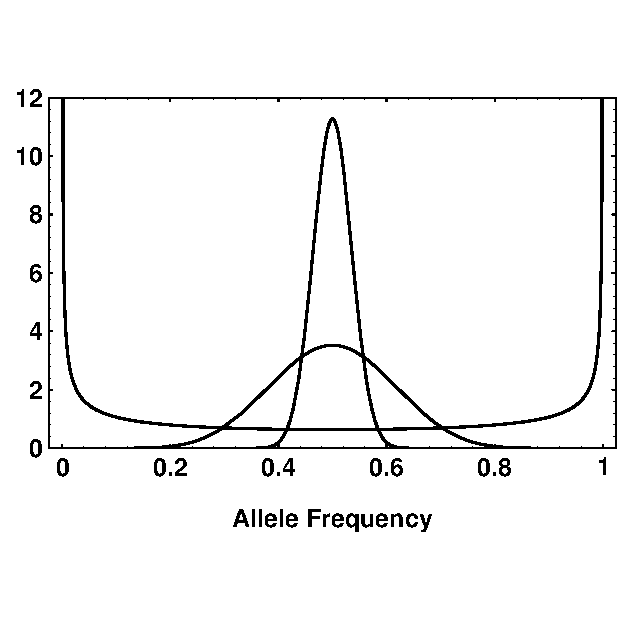
\includegraphics{mutation.eps}}
\end{center}
\caption{The stationary distribution of allele frequencies for one
  locus and two alleles with symmetrical mutation.}\label{fig:drift-mutation}
\end{figure}

When $4N\mu < 1$ the stationary distribution of allele frequencies is
bowl-shaped, i.e, most populations have allele frequencies near 0 or
1. When $4N\mu > 1$, the stationary distribution of allele frequencies
is hump-shaped, i.e., most populations have allele frequencies near
0.5.\footnote{Notice again that it's the product of $N$ and $\mu$ that
  matters.} In other words if the population is ``small,'' drift
dominates the distribution of allele frequencies and causes
populations to become differentiated. If the population is ``large,''
mutation dominates and keeps the allele frequencies in the different
populations similar to one another. That's what we mean when we say
that a population is ``large'' or ``small''. A population is ``large''
if evolutionary processes other than drift have a predominant
influence on the outcome. It's ``small'' if drift has a predominant
role on the outcome.\index{genetic drift!population size}

A population is large with respect to the drift-mutation process if
$4N\mu > 1$, and it is small if $4N\mu < 1$. Notice that calling a
population large or small is really just a convenient shorthand. There
isn't much of a difference between the allele frequency distributions
when $4N\mu = 0.9$ and when $4N\mu = 1.1$. Notice also that because
mutation is typically rare, on the order of $10^{-5}$ or less per
locus per generation for a protein-coding gene, a population must be
pretty large ($> 25,000$) to be considered large with respect to
drift and mutation. Notice also that whether the population is ``large''
or ``small'' will depend on the mutation rate at the loci that you're
studying. For example, mutation rates are typically on the order of 
$10^{-3}$ for microsatellites. So a population would be ``large'' with
respect to microsatellites if $N > 250$. Think about what that
means. If we had a population with 1000 individuals, it would be
``large'' with respect to microsatellite evolution and ``small'' with
respect to evolution at a protein-coding locus.

\section*{Drift and migration}\index{genetic drift!migration}

I just pointed out that if populations are isolated from one another
they will tend to diverge from one another as a result of genetic
drift. Recurrent mutation, which ``pushes'' all populations towards
the same allele frequency, is one way in which that tendency can be
opposed. If populations are not isolated, but exchange migrants with
one another, then migration will also oppose the tendency for
populations to become different from one another. It should be obvious
that there will be a tradeoff similar to the one with mutation: the
larger the populations, the less the tendency for them to diverge from
one another and, therefore, the more migration will tend to make them
similar. To explore how drift and migration interact we can use an
approach exactly analogous to what we used for mutation.

The model of migration we'll consider is an extremely oversimplified
one. It imagines that every allele brought into a population is
different from any of the resident alleles.\footnote{Sounds a lot like
  the infinite alleles model of mutation, doesn't it? Just you
  wait. The parallel gets even more striking.} It also imagines that
all populations receive the same fraction of migrants. Because any
immigrant allele is different, by assumption, from any resident allele
we don't even have to keep track of how far apart populations are from
one another, since populations close by will be no more similar to one
another than populations far apart. This is Wright's infinite island
model of migration. Given these assumptions, we can write the
following:
\begin{equation}
f_{t+1} = \left(\left(\frac{1}{2N}\right) +
          \left(1 - \frac{1}{2N}\right)f_t\right)(1-m)^2 \quad
\label{eq:f-m} .
\end{equation}

That might look fairly familiar. In fact, it's identical to equation
(\ref{eq:f-mu}) except that there's an $m$ in (\ref{eq:f-m}) instead
of a $\mu$. $m$ is the migration rate, the fraction of individuals in
a population that is composed of immigrants. More precisely, $m$ is
the {\it backward\/} migration rate.\index{migration rate!backward}
It's the probability that a randomly chosen individual in this
generation {\it came from\/} a population different from the one in
which it is currently found in the preceding generation. Normally we'd
think about the {\it forward\/} migration rate,\index{migration rate!forward}  i.e., the probability
that a randomly chosen individual with {\it go to\/} a different
population in the next generation, but backwards migration rates turn
out to be more convenient to work with in most population genetic
models.\footnote{I warned you weeks ago that population geneticists
  tend to think backwards.}

It shouldn't surprise you that if equations (\ref{eq:f-mu}) and
(\ref{eq:f-m}) are so similar the equilibrium $f$ under drift and
migration is
\[
\hat f \approx \frac{1}{4Nm + 1}
\]
In fact, the two allele analog to the mutation model I presented
earlier turns out to be pretty similar, too.

\begin{itemize}

\item If $2Nm > 1$, the stationary distribution of allele frequencies
is hump-shaped, i.e., the populations tend not to diverge from one
another.\footnote{You read that right it's $2Nm$ not $4Nm$ as you
might have expected from the mutation model. If you're {\it really\/}
interested why there's a difference, I can show you. But the
explanation isn't simple.}

\item If $2Nm < 1$, the stationary distribution of allele frequencies
is bowl-shaped, i.e., the populations tend to diverge from one another.

\end{itemize}

Now there's a consequence of these relationships that's both
surprising and odd. $N$ is the population size. $m$ is the fraction of
individuals in the population that are immigrants. So $Nm$ is the {\it
  number\/} of individuals in the population that are new immigrants
in any generation. That means that if populations receive more than
one new immigrant every other generation, on average, they'll tend not
to diverge in allele frequency from one another.\footnote{In the sense
  that the stationary distribution of allele frequencies is
  hump-shaped.} It doesn't make any difference if the populations have
a million individuals apiece or ten. One new immigrant every other
generation is enough to keep them from diverging.

With a little more reflection, this result is less surprising than it
initially seems. After all in populations of a million individuals,
drift will be operating very slowly, so it doesn't take a large
proportion of immigrants to keep populations from
diverging.\footnote{And one immigrant every other generation
  corresponds to a backwards migration rate of only $5\times
  10^{-7}$.} In populations with only ten individuals, drift will be
operating much more quickly, so it takes a large proportion of
immigrants to keep populations from diverging.\footnote{And one
  immigrant every other generation corresponds to a backwards
  migration rate of $5 \times 10^{-2}$.}

\ccLicense

\end{document}

\documentclass[12pt]{article}
\usepackage{lecture}
\usepackage{html}
\usepackage{url}
\usepackage{graphics}

\title{Selection and genetic drift}

\newcommand{\copyrightYears}{2001-2021}

\begin{document}

\maketitle

\thispagestyle{first}

\section*{Introduction}

There are three basic facts about genetic drift that I really want you
to remember, even if you forget everything else I've told you about
it:

\begin{enumerate}

\item Allele frequencies tend to change from one generation to the
next purely as a result of random sampling error. We can specify a
probability distribution for the allele frequency in the next
generation, but we cannot specify the numerical value exactly.

\item There is no systematic bias to the change in allele frequency,
i.e., allele frequencies are as likely to increase from one generation
to the next as to decrease.

\item Populations will eventually fix for one of the alleles that is
initially present unless mutation or migration introduces new
alleles. 

\end{enumerate}

Natural selection introduces a systematic bias in allele frequency
changes. Alleles favored by natural selection {\it tend\/} to increase
in frequency. Notice that word ``tend.'' It's critical. Because there
is a random component to allele frequency change when genetic drift is
involved, we can't say for sure that a selectively favored allele will
increase in frequency. In fact, we can say that there's a chance that
a selectively favored allele {\it won't\/} increase in
frequency. There's also a chance that a selectively {\it dis\/}favored
allele will increase in frequency in spite of natural selection.

\section*{Loss of beneficial alleles}\index{genetic drift!loss of beneficial alleles}

We're going to confine our studies to our usual simple case: one
locus, two alleles. We're also going to consider a very simple form of
directional viability selection in which the heterozygous genotype is
exactly intermediate in fitness.\footnote{Note that if the absolute
  viabilities of $A_1A_1$, $A_1A_2$, and $A_2A_2$ are $w_{11}$,
  $w_{12}$, and $w_{22}$ respectively, then we can write the relative
  fitnesses as $1+s$, $1+hs$, and $1$. We're considering the special
  case where $h=1/2$.}

\begin{center}
\begin{tabular}{ccc}
$A_1A_1$ & $A_1A_2$      & $A_2A_2$ \\
1 + s    & $1 + \half s$ & 1
\end{tabular}
\end{center}

After solving a reasonably complex partial differential equation, it
can be shown that\footnote{Remember, I told you that ``it can be shown
that'' hides a {\it lot\/} of work.} the probability that allele
$A_1$\footnote{The beneficial allele.}  is fixed, given that its
current frequency is $p$ is
\begin{equation}
P_1(p) = \frac{1 - e^{-2N_esp}}{1 - e^{-2N_es}} \quad .
\label{eq:beneficial}
\end{equation}
Now it won't be immediately evident to you, but this equation actually
confirms our intuition that even selectively favored alleles may
sometimes be lost as a result of genetic drift. How does it do that?
Well, it's not too hard to verify that $P_1(p) < 1$.\footnote{Unless
  $p=1$.} The probability that the beneficial allele is fixed is less
than one meaning that the probability it is lost is greater than zero,
i.e., there's some chance it will be lost.

How big is the chance that a favorable allele will be
lost?\index{genetic drift!fixation probability} Well, consider the
case of a newly arisen allele with a beneficial effect. If it's newly
arisen, there is only one copy by definition. In a diploid population
of $N$ individuals that means that the frequency of this allele is
$1/2N$. Plugging this into equation (\ref{eq:beneficial}) above we
find
\begin{eqnarray*}
P_1(p) &=& \frac{1 - e^{-2N_es(1/2N)}}{1 - e^{-2N_es}} \\
       &\approx& 1 - e^{-N_es(1/N)} \hbox{ if $2N_es$ is ``large''} \\
       &=& 1 - e^{s\left(\frac{N_e}{N}\right)} \\
       &\approx& s\left(\frac{N_e}{N}\right)
                 \hbox{ if $s$ is ``small.''}
\end{eqnarray*}
In other words, most beneficial mutations are lost from populations
unless they are {\it very\/} beneficial.\footnote{Notice that it's the
  product of $N_e$ and $s$ that matters, not either one by
  itself. Thus, a population is ``large'' with respect to selection if
  $2N_es > 1$.} If $s=0.2$ in an ideal population, for example, a
beneficial mutation will be lost about 80\% of the time.\footnote{The
  exact calculation from equation (\ref{eq:beneficial}) gives 82\% for
  this probability.} Remember that in a strict harem breeding system
with a single male $N_e \approx 4$ if the number of females with which
the male breeds is large enough. Suppose that there are 99 females in
the population. Then $N_e/N = 0.04$ and the probability that this
beneficial mutation will be fixed is only 0.8\%.

Notice that unlike what we saw with natural selection when we were
ignoring genetic drift, the strength of selection\footnote{i.e., the
  magnitude of differences in relative viabilities} affects the
outcome of the interaction. The stronger selection is the more likely
it is that the favored allele will be fixed. In the case of a newly
arisen allele, it's also {\it only\/} the strength of selection that
matters. Since a newly arisen allele is, by definition exists as only
a single copy, it is very likely to be lost by chance. Once an a
favorable allele has reached an appreciable frequency, the larger the
population is, the more likely the favored allele will be
fixed.\footnote{Because the larger the population, the smaller the
  effect of drift.} Size {\it does\/} matter. But most favorable
alleles are lost before they increase in frequency enough for the
population size to matter.

\section*{Fixation of detrimental alleles}\index{genetic drift!fixation of deleterious alleles}

If drift can lead to the loss of beneficial alleles, it should come as
no surprise that it can also lead to fixation of deleterious ones. In
fact, we can use the same formula we've been using (equation
(\ref{eq:beneficial})) if we simply remember that for an allele to be
deleterious $s$ will be negative. So we end up with
\begin{equation}
P_1(p) = \frac{1 - e^{2N_esp}}{1 - e^{2N_es}} \quad .
\label{eq:deleterious}
\end{equation}
One implication of equation (\ref{eq:deleterious}) that should not be
surprising by now is that even a deleterious allele can become
fixed.\footnote{You might be wondering why I'm not using the same
  approximation here as I did in equation~(\ref{eq:beneficial}), since
  the equations look so similar. The reason is that the exponent on
  $e$ in the denominator is now positive. So $e^{2N_es}$ is the
  biggest term in the denominator instead of the smallest, meaning
  that we can't neglect it.} Consider our two example populations
again, an ideal population of size 100 ($N_e = 100$) and a population
with 1 male and 99 females ($N_e = 4$). Remember, the probability of
fixation for a newly arisen allele allele with no effect on fitness is
$1/2N = 5 \times
10^{-3}$~(Table~\ref{table:fixation}).\footnote{Because
  it's probability of fixation is equal to its current frequency,
  i.e., $1/2N$. We'll return to this observation in a few weeks when
  we talk about the neutral theory of molecular evolution.}

\begin{table}
\begin{center}
\begin{tabular}{l|cc}
\hline\hline
      & \multicolumn{2}{c}{$N_e$} \\
$s$   & 4                  & 100 \\
\hline
0.001 & $4.9 \times 10^{-3}$ & $4.5 \times 10^{-3}$ \\
0.01  & $4.8 \times 10^{-3}$ & $1.5 \times 10^{-3}$ \\
0.1   & $3.2 \times 10^{-3}$ & $2.2 \times 10^{-10}$ \\
\hline
\end{tabular}
\end{center}
\caption{Fixation probabilities for a deleterious mutation as a
function of effective population size and selection coefficient for a
newly arisen mutant ($p=0.01$).}\label{table:fixation}
\end{table}

\section*{Genetic drift and heterozygote advantage}\index{genetic drift!heterozygote advantage}

\begin{itemize}

\item Genetic drift leads to the loss of genetic diversity over time. 

\item Heterozygote advantage leads to the preservation of genetic diversity.

\end{itemize}

You might think that those facts would lead to the conclusion that
drift would cause there to be less diversity than expected as a result
of selection, but that selection would maintain diversity. It would be
nice if the world were that simple. Unfortunately, it's not. 

The key to understanding why is to remember this basic fact: In a
finite population there is a chance that in any generation one of the
alleles that is segregating will be lost. In the absence of mutation
or migration that introduces new genetic diversity into a finite
population, that allele is lost forever. The end result is that {\it
  any\/} finite population will eventually lose its genetic diversity
in the absence of mutation or migration, even one in which selection
is ``trying'' to maintain diversity. Once you realize that, then you
realize that the question isn't ``Will heterozygote advantage maintain
genetic diversity in spite of genetic drift?'' but ``Will heterozygote
advantage retard the inevitable loss of genetic diversity due to
genetic drift?'' The answer to that second questions is ``It depends.''

Specifically, Robertson~\cite{Robertson-1962} showed that if selection
would lead to an equilibrium allele frequency of between about 0.2 and
0.8, then it will tend to retard the loss of genetic diversity. If,
however, selection would lead to a more extreme allele frequency, it
will tend to increase the rate at which diversity is
loss~(Figure~\ref{fig:drift-heterozygote-advantage}). While that
result seems paradoxical at first, after a bit of reflection, it's
somewhat less surprising.

\begin{itemize}

\item If an allele is relatively rare, drift will tend to dominate the
  dynamics of allele frequency change, even if it's under selection.

\item If selection is ``pushing'' an allele to a relatively extreme
  frequency, it will get to the region where drift dominates the
  dynamics more rapidly than it would under drift alone.

\item So heterozygote advantage in which the two homozygotes have very
  asymmetrical fitnesses is likely to increase the rate at which
  diversity is lost. As a corollary, the allele in the disfavored
  homozygote is the most likely to be lost.

\end{itemize}

\begin{figure}
\begin{center}
\resizebox{!}{6cm}{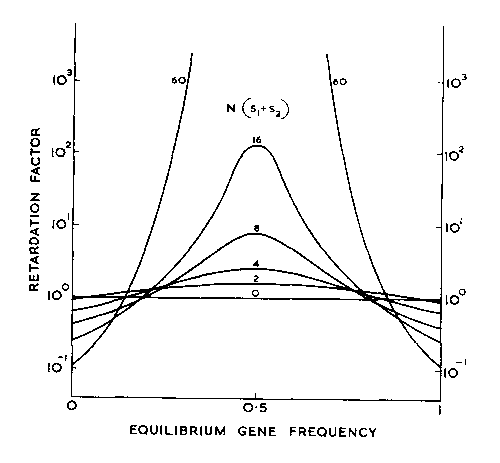
\includegraphics{drift-heterozygote-advantage.eps}}
\end{center}
\caption{The ``retardation factor'' as a function of the equilibrium
  frequency under selection alone and the strength of selection,
  $N(s_1+s_2)$~(from~\cite{Robertson-1962}).}\label{fig:drift-heterozygote-advantage} 
\end{figure}

\section*{Genetic draft}\index{genetic draft}

No. That's not a typo. I meant to type ``genetic draft.'' Genetic
draft is a term that John Gillespie coined~\cite{Gillespie-2000} to
describe a phenomenon similar to genetic drift: If there is ``a steady
stream of adaptive substitutions at one locus$\dots$, [then] the
induced stochastic effects of the substitutions on [a linked] neutral
locus can be faithfully captured in a one-locus model called the {\it
  pseudohitchhiking model}''~\cite[p. 909]{Gillespie-2000} He shows
that the neutral locus shows dynamics that are quite different from
what would be expected if it were not linked to the selective
locus. The effects are illustrated in Figure~\ref{fig:genetic-draft}

\begin{figure}
\begin{center}
\resizebox{!}{8cm}{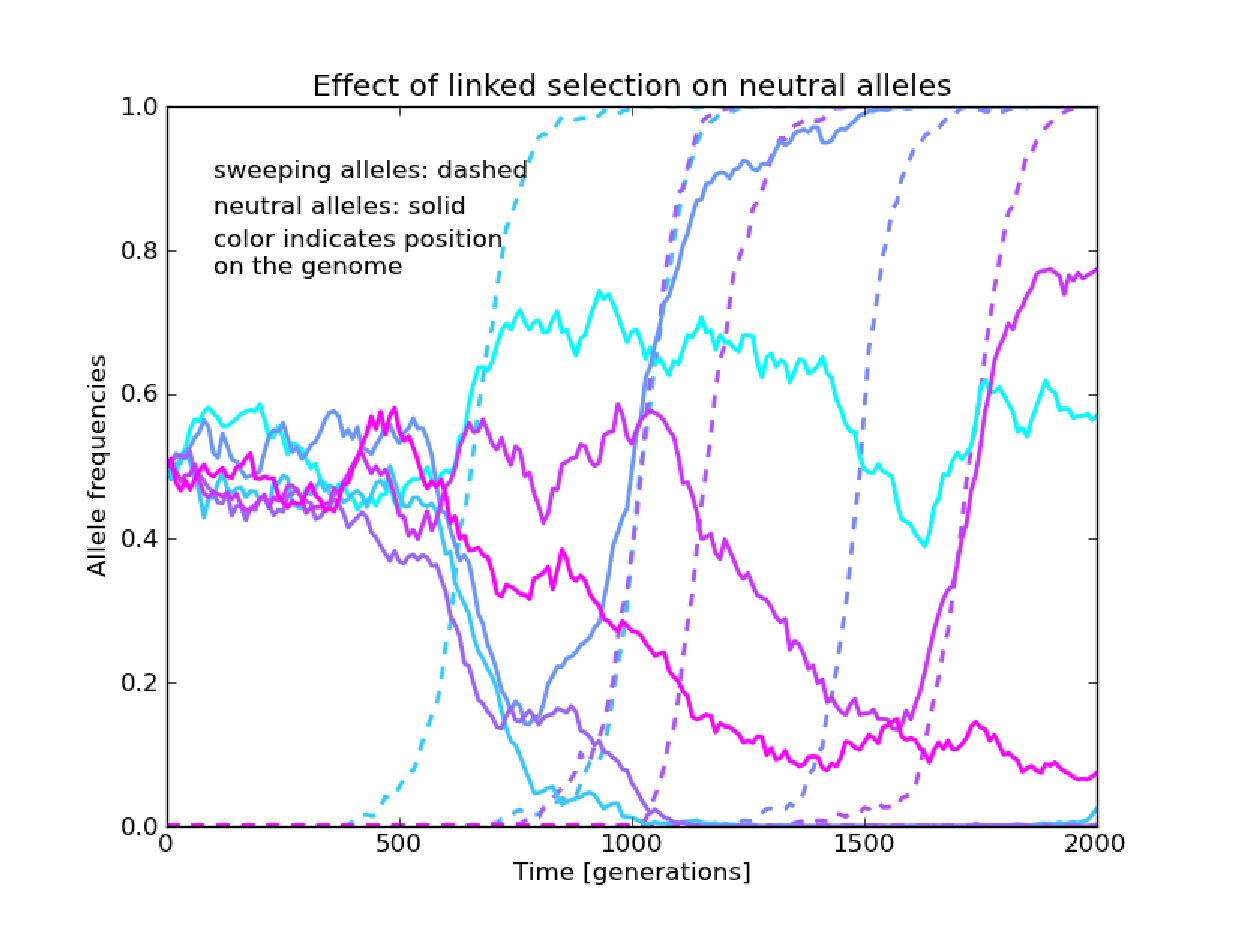
\includegraphics{genetic-draft.eps}}
\end{center}
\caption{The color indicates the position on the genome, selected
  trajectories are in shown as dashed lines, neutral ones by solid
  lines. Neutral allele frequencies are most strongly perturbed by
  sweeps nearby on the chromosome, i.e., of similar color~(from
  {\tt http://webdav.tuebingen.mpg.de/interference/draft.html};
  accessed 27 February 2017).}\label{fig:genetic-draft}  
\end{figure}

\section*{Conclusions}

There are four properties of the interaction of drift and selection
that I think you should take away from this brief
discussion:\index{genetic drift!properties with selection}

\begin{enumerate}

\item Most mutations, whether beneficial, deleterious, or neutral, are
  lost from the population in which they occurred.

\item If selection against a deleterious mutation is weak or $N_e$ is
  small,\footnote{As with mutation and migration, what counts as large
    or small is determined by the product of $N_e$ and $s$. If it's
    bigger than one the population is regarded as large, because
    selective forces predominate. If it's smaller than one, it's
    regarded as small, because drift predominates.} a deleterious
  mutation is almost as likely to be fixed as neutral mutants. They
  are ``effectively neutral.''\index{effectively neutral}\index{genetic drift!effectively neutral}\footnote{We'll
    come back to ``effectively neutral'' when we discuss the neutral
    theory of molecular evolution. It's a very important concept that
    has broader implications than you might guess.}

\item If $N_e$ is large, deleterious mutations are much less likely to
  be fixed than neutral mutations.

\item Even if $N_e$ is large, most favorable mutations are lost.

\item If selection favors heterozygotes, it will retard the loss of
  genetic diversity only when the fitnesses of the two homozygotes are
  not greatly different from one another.

\end{enumerate}

\bibliography{popgen}
\bibliographystyle{plain}

\ccLicense

\end{document}

\documentclass[12pt]{article}
\usepackage{lecture}
\usepackage{html}
\usepackage{url}
\usepackage{graphics}
\usepackage{epstopdf}

\newcommand{\copyrightYears}{2001-2021}

\title{The Coalescent}

\begin{document}

\maketitle

\thispagestyle{first}

\section*{Introduction}

I've mentioned many times by now that population geneticists often
look at the world backwards. To those of you who aren't population
geneticists,\footnote{i.e., virtually everyone who is reading these
  notes.} looking at the world backwards is probably as awkwards as
walking backwards. Sometimes, though, it turns out that walking
backwards is useful, as when you're trying to keep an eye on where
you've been, not just where you're going. That's what we're about to
do with genetic drift. So far we've been trying to predict what will
happen in a population given a particular effective population
size. But when we collect data we are often more interested in
understanding the processes that produced the pattern we find than in
predicting what will happen in the future. We're using data to provide
insight about where we've been, not where we're going. So let's take a
backward look at drift and see what we find.


\section*{Reconstructing the genealogy of a sample of
  alleles}\index{allele genealogy}\index{coalescent}

Specifically, let's keep track of the genealogy of alleles. In a
finite population, two randomly chosen alleles will be identical by
descent with respect to the immediately preceding generation with
probability $1/2N_e$. That means that there's a chance that two
alleles in generation $t$ are copies of the same allele in generation
$t-1$. If the population size is constant, meaning that the number of
allele copies\footnote{I'm using the phrase ``allele copy'' here to
  refer to distinct physical alleles. Allele copies may or may not be
  identical by type or identical by descent. If a diploid population
  has effective size $N_e$, then the number of allele {\it copies\/}
  is $2N_e$. The number of allele types may be 1, 2, or any other
  integer less than or equal to $2N_e$. Similarly, the number of
  identity by descent categories among the alleles may be anything rom
  1 to $2N_e$.}\index{allele copy} is also constant, that also means
that there's a chance that some allele copies present in generation
$t-1$ will not have descendants in generation $t$. Looking backward,
then, the number of allele copies in generation $t-1$ that have
descendants in generation $t$ is always less than or equal to the
number of allele copies in generation $t$. That means if we trace the
ancestry of allele copies in a sample back far enough, all of them
will be descended from a single common ancestor.\footnote{As you can
  see, it quickly becomes tedious to write ``allele copies.'' I'm
  going to write ``allele'' throughout the rest of this
  discussion. Just remember that when I do, I'm really referring to an
  allele copy.}  Figure~\ref{fig:coalescent} provides a simple
schematic illustrating how this might happen.

\begin{figure}
\begin{center}
\resizebox{!}{5cm}{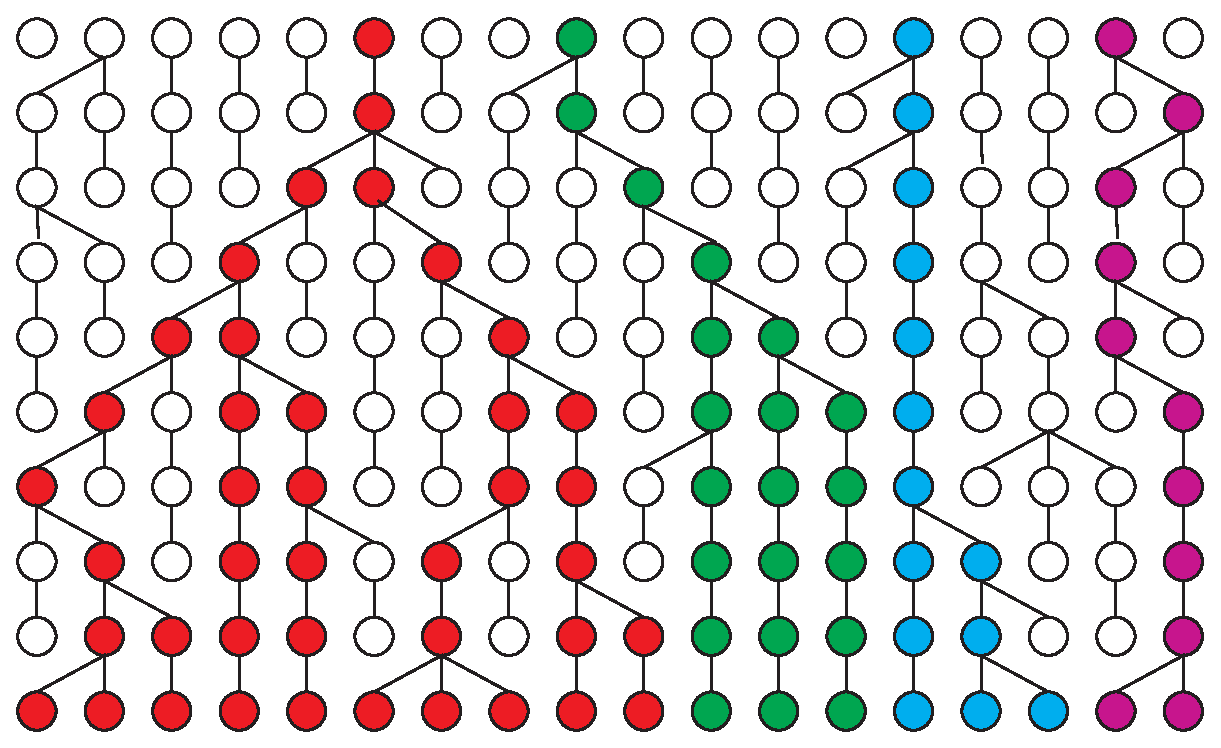
\includegraphics{coalescent-figure.eps}}
\end{center}
\caption{A schematic depiction of one possible realization of the
  coalescent process in a population with 18 haploid gametes. There
  are four coalescent events in the generation immediately preceding
  the last one illustrated, one involving three alleles.}\label{fig:coalescent}
\end{figure}

Time runs from the top of Figure~\ref{fig:coalescent} to the bottom,
i.e., the current generation is represented by the circles in the
botton row of the figure. Each circle represents an allele. The
eighteen alleles in our current sample are descended from only four
alleles that were present in the populations ten generations ago. The
other fourteen alleles present in the population ten generations ago
left no descendants. How far back in time we'd have to go before all
alleles are descended from a single common ancestor depends on the
effective size of the population, because how frequently two (or more)
alleles are descended from the same allele in the preceding generation
depends on the effective size of the population, too. But in any
finite population the pattern will look something like the one I've
illustrated here.

\section*{Mathematics of the coalescent: two
  alleles\footnote{Remember, I'm
  talking about allele copies here.}}\index{coalescent!two alleles}

The mathematician J. F. C. Kingman developed a convenient and powerful
way to describe how the time to common ancestry is related to
effective population
size~\cite{Kingman-1982-genealogy,Kingman-1982-coalescent}. The
process he describes is referred to as the {\it coalescent}, because
it is based on describing the probability of {\it coalescent
  events},\index{coalescent events} i.e., those points in the
genealogy of a sample of alleles where two alleles are descended from
the same allele in the immediately preceding generation.\footnote{An
  important assumption of the coalescent is that populations are large
  enough that we can ignore the possibility that there is more than
  one coalescent event in a single generation. That also means that we
  also only allow coalescence between a pair of alleles, not three or
  more. In both ways the mathematical model of the process differs
  from the diagram in Figure~\ref{fig:coalescent}.}  Let's consider a
simple case, one that we've already seen, e.g., two alleles
drawn at random from a single population.

The probability that two alleles drawn at random from a population are
copies of the same allele in the preceding generation is also the
probability that two alleles drawn at random from that population are
identical by descent with respect to the immediately preceding
generation. We know what that probability is,\footnote{Though you may
not remember it.} namely
\[
\frac{1}{2N_e^{(f)}} \quad .
\]
I'll just use $N_e$ from here on out, but keep in mind that the
appropriate population size for use with the coalescent is the
inbreeding effective size. Of course, this means that the probability
that two alleles drawn at random from a population are {\it not\/}
copies of the same allele in the preceding generation is
\[
1 - \frac{1}{2N_e} \quad .
\]
We'd like to calculate the probability that a coalescent event
happened at a particular time $t$, in order to figure out how far back
in the ancestry of these two alleles we have to go before they have a
common ancestor. How do we do that?

Well, in order for a coalescent event to occur at time $t$, the two
alleles must have {\it not\/} have coalesced in the generations
preceding that.\footnote{Remember that we're counting generations
  backward in time, so when I say that a coalescent event occurred at
  time $t$ I mean that it occurred $t$ generations ago.} The
probability that they did not coalesce in the first $t-1$ generations
is simply
\[
\left(1 - \frac{1}{2N_e}\right)^{t-1} \quad .
\]
Then after having remained distinct for $t-1$ generations, they have
to coalesce in generation $t$, which they do with probability
$1/2N_e$. So the probability that two alleles chosen at random
coalesced $t$ generations ago is
\begin{equation}
P(T=t) = \left(1 -
\frac{1}{2N_e}\right)^{t-1}\left(\frac{1}{2N_e}\right) \quad .
\label{eq:two-allele}
\end{equation}
It's not too hard to show, once we know the probability distribution
in equation (\ref{eq:two-allele}), that the average time to
coalescence for two randomly chosen alleles is $2N_e$.\footnote{If
  you've had a little bit of probability theory, you'll notice that
  equation~\ref{eq:two-allele} shows that the coalescence time is a
  geometric random variable.}\index{coalescent!time to common ancestry}

\section*{Mathematics of the coalescent: multiple
  alleles}\index{coalescent!multiple alleles}

It's quite easy to extend this approach to multiple
alleles.\footnote{Okay, okay. What I should really have said is ``It's
  not {\it too\/} hard to extend this approach to multiple alleles, if
  you are comfortable with probability thinking.'' Remember: I don't
  expect you to be able to derive these results on your own. Don't
  worry if you can't see how you could have come up with the
  mathematics that follow. Unless you want to make contributions to
  developing new theory in population genetics, you don't need to do
  derivations like these. Nonetheless, I think it's useful for you to
  see them. That way you have a better chance of understanding the
  limitations of coalescence approaches if you use them in analyzing
  your own data.}  We're interested in seeing how far back in time we
have to go before all alleles are descended from a single common
ancestor. We'll assume that we have $m$ alleles in our sample. The
first thing we have to calculate is the probability that any two of
the alleles in our sample are identical by descent from the
immediately preceding generation. To make the calculation easier, we
assume that the effective size of the population is large enough that
the probability of two coalescent events in a single generation is
vanishingly small. We already know that the probability of a
coalescence in the immediately preceding generation for two randomly
chosen alleles is $1/2N_e$. But there are $m(m-1)/2$ different pairs
of alleles in our sample.\footnote{Where did I get that $m(m-1)/2$?
  You can either take my word for it as ``a well known fact,'' or you
  can ask me about it, and I'll show you where it comes from.} So the
probability that one pair of these alleles is involved in a coalescent
event in the immediately preceding generation is
\begin{equation}
  \left(\frac{1}{2N_e}\right)\left(\frac{m(m-1)}{2}\right) \quad .
  \label{eq:multi-allele-first-event}
\end{equation}
From this it follows\footnote{Using logic just like what we used in
the two allele case.} that the probability that the first coalescent
event involving this sample of alleles occurred $t$ generations ago is
\begin{equation}
P(T=t) =
\left(1-\left(\frac{1}{2N_e}\right)\left(\frac{m(m-1)}{2}\right)\right)^{t-1}
\left(\frac{1}{2N_e}\right)\left(\frac{m(m-1)}{2}\right)
\quad .
\label{eq:multi-allele}
\end{equation}
So the mean time back to the first coalescent event is
\[
\frac{2N_e}{m(m-1)/2} = \frac{4N_e}{m(m-1)} \hbox{ generations} \quad .
\]

But this is, of course, only the first coalescent event. We were
interested in how long we have to wait until {\it all\/} alleles are
descended from a single common ancestor. Now this is where Kingman's
sneaky trick comes in. After the first coalescent event, we have $m-1$
alleles in our sample, instead of $m$. So the whole process starts
over again with $m-1$ alleles instead of $m$.\footnote{For anyone who
  cares, this is another example of the Markov property of genetic
  drift.}\index{genetic drift!Markov property} Since the time to the
first coalescence depends only on the number of alleles in the sample
and not on how long the first coalescence event took, we can calculate
the average time until all coalescences have happened
as\index{coalescent!time to coalescence}
\begin{eqnarray*}
\bar t &=& \sum_{k=2}^m \bar t_k \\
       &=& \sum_{k=2}^m \frac{4N_e}{k(k-1)} \\
       && \mbox{TAMO} \\
       &=& 4N_e\left(1 - \frac{1}{m}\right) \\
       &\approx& 4N_e
\end{eqnarray*}

\subsection*{A continuous time version of the coalescent}

Since the effective size of a population has to be pretty big for the
coalescent process to be a good representation, big enough that
$(1/2N_e)^2$ is negligible, $4N_e$ is generally in the hundreds or
thousands. That means that even though the coalescent as I formulated
it above is a discrete time process, i.e., events happen at time 1, 2,
3, $\dots$, it can be convenient to think of time as continuous, which
is surprisingly easy to do. We start with the ``well-known fact'' that
if $p$ is ``small''
\[
\log(1-p) \approx -p \quad .
\]
As a result,
\begin{eqnarray*}
(1 - p)^t &=& e^{t \log(1-p)} \\
          &\approx& e^{-pt} \quad .
\end{eqnarray*}
In our case,
\[
p = \frac{k(k-1)}{4N_e} \quad ,
\]
when there are $k$ alleles.\footnote{Remember, I'm using ``alleles''
  as shorthand for ``allele copies'' (and wasting a lot more space
  with this footnote than I would have if I'd just written ``allele
  copies'' in the text).} So
\[
t_k = \left(\frac{k(k-1)}{4N_e}\right)e^{{(t-1)}{\frac{k(k-1)}{4N_e}}} \quad .
\]


\subsection*{An example: Mitochondrial
  Eve}\index{coalescent!mitochondrial Eve}

Cann et al.~\cite{Cann-etal-1987} sampled mitochondrial DNA from 147
humans of diverse racial and geographic origins.\footnote{That may
  seem like a pretty small sample to you, but the technology
  available to analyze genomes has advanced tremendously since Cann et
  al. did their work. To sequence a segment of DNA for example,
  required, among other things, running samples on a polyacrylamide
  gel, producing an autoradiogram, and manually reading the
  results. The process took about 2 weeks per sequence.}  Based on the
amount of sequence divergence they found among genomes in their sample
and independent estimates of the rate of sequence evolution, they
inferred that the mitochondria in their sample had their most recent
common ancestor about 200,000 years ago. Because all of the most
ancient lineages in their sample were from individuals of African
ancestry, they also suggested that mitochondrial Eve lived in
Africa. They used these arguments as evidence for the ``Out of
Africa'' hypothesis for modern human origins, i.e., the hypothesis
that anatomically modern humans arose in Africa about 200,000 years
ago and displaced other members of the genus {\it Homo\/} in Europe
and Asia as they spread. What does the coalescent tell us about their
conclusion?

Well, we expect all mitochondrial genomes in the sample to have had a
common ancestor about $2N_e$ generations ago. Why $2N_e$ rather than
$4N_e$? Because mitochondrial genomes are haploid, not
diploid. Furthermore, since we all get our mitochondria from our
mothers,\footnote{Luo et al.~\cite{Luo-etal-2018} recently presented
  data suggesting that mitochondria may sometimes be biparentally
  inherited in humans and that whether or not biparental inheritance
  occurs seems to be determined by the nuclear genotype of the
  mother.} $N_e$ in this case refers to the effective number of {\it
  females}.

Given that a human generation is about 20 years, a coalescence time of
200,000 years implies that the mitochondrial genomes in the Cann et
al. sample have their most recent common ancestor about 10,000
generations ago. If the effective number of females in the human
populations is 5000, that's exactly what we'd expect. While 5000 may
sound awfully small, given that there are more than 3 billion women on
the planet now, remember that until the recent historical past (no
more than 500 generations ago) the human population was small and
humans lived in small hunter-gatherer groups, so an effective number
of females of 5000 and a total effective size of 10,000 may not be
unreasonable. If that's true, then the geographical location of
mitochondrial Eve need not tell us anything about the origin of modern
human populations, because there had to be a coalescence
somewhere. There's no guarantee, from this evidence alone, that the
Y-chromosome Adam would have lived in Africa, too. Having said that,
my limited reading of the literature suggests that more extensive
recent data are consistent with the ``Out of Africa''
scenario. Y-chromosome polymorphisms, for example, are also consistent
with the ``Out of Africa''
hypothesis~\cite{Underhill-etal-2000}. Interestingly, dating of
Y-chromosome polymorphisms suggests that Y-chromosome Adam left
Africa only 35,000 -- 89,000 years ago.

\section*{The coalescent and $F$-statistics}\index{F-statistics@$F$-statistics!coalescent}\index{coalescent!F-statistics@$F$-statistics}

Suppose we have a sample of alleles from a structured population. For
alleles chosen randomly within populations, let the average time to
coalescence be $\bar t_0$. For alleles chosen randomly from different
populations, let the average time to coalescence be $\bar t_1$. If
there are $k$ populations in our sample, the average time to
coalescence for two alleles drawn at random without respect to
population is\footnote{If you don't see why, don't worry about it. You
can ask if you really care. We only care about $\bar t$ for what
follows anyway.}
\begin{eqnarray*}
  \bar t &=& \frac{1}{k}\bar t_0 + \frac{k-1}{k}\bar t_1 \\
  &=& \frac{\bar t_0 + (k-1)\bar t_1}
              {k} \quad .
\end{eqnarray*}
Slatkin~\cite{Slatkin-1991} pointed out that $F_{st}$ bears a simple
relationship to average coalescence times within and among
populations. Given these definitions of $\bar t$ and $\bar t_0$,
\begin{eqnarray*}
  F_{st} &=& \frac{\bar t - \bar t_0}{\bar t} \quad .
\end{eqnarray*}
So another way to think about $F_{st}$ is as a measure of the
proportional increase in coalescence time that is due to populations
being separate from one another. One way to think about that
relationship is this: the longer it has been, on average, since
alleles in different populations diverged from a common ancestor, the
greater the chance that they have become different. An implication of
this relationship is that $F$-statistics, by themselves, can tell us
something about how recently populations have been connected, relative
to the within-population coalescence time, but they can't distinguish
between recent common ancestry that is due to migration among
populations and recent common ancestry that is due to a split between
populations.

A given pattern of among-population relationships might reflect a
migration-drift equilibrium, a sequence of population splits followed
by genetic isolation, or any combination of the two. If we are willing
to assume that populations in our sample have been exchanging genes
long enough to reach stationarity in the drift-migration process, then
$F_{st}$ may tell us something about migration. If we are willing to
assume that there's been no gene exchange among our populations, we
can infer something about how recently they've diverged from one
another. But unless we're willing to make one of those assumptions, we
can't really say anything.\index{genetic drift!migration}\footnote{We can't say anything from allele
  frequencies alone. If we have DNA sequences for the alleles, which
  allow us to tell how closely related they are to one another, we
  can say something. We'll get to this when we discuss phylogeography
  in a few weeks.}

\section*{The coalescent and natural selection}\index{coalescent!natural selection}

It shouldn't surprise you that if we can study some of the properties
of drift and selection, we can also use the coalescent to understand
how natural selection works in a finite population. Even though the
mathematics of the coalescent are ususally simpler than the older
diffusion approach for studying allele frequency changes in a finite
population, they are still very complicated. I'll simply outline one
approach here known as the {\it structured
  coalescent}.\index{structured coalescent} 

The idea is reasonably simple, especially if we think about selection
involving only two alleles.\footnote{Wakeley~\cite{Wakeley-2010}
  provides a reasonably accessible overview. Coop and
  Griffiths~\cite{Coop-Griffiths-2004} provide all of the gory
  details.} When you start to think about it, you should realize two
things pretty quickly:

\begin{enumerate}

  \item Coalescent events will happen only {\it within} each of the
    two allele classes. If we were to trace the history back far
    enough, to the point where the mutation leading to a second allele
    occurred, then there might be coalescence involving the two
    classes{\dash}except that there wouldn't be two classes, only
    one.

  \item The allele copies\footnote{There's that phrase again.} within
    one of the two allele classes will all have the same fitness
    properties. That means that the genealogy within each allele
    classs will behave just like the coalescent you've already seen.
    
 \end{enumerate}
There are a couple of further complications. The first one is that the
probability of a coalescent event between two alleles belonging to an
allele class whose frequency is $p_t$ is
\[
 \frac{\frac{m(m-1)}{2}}{2N_ep_t} \quad .
 \]
If you think about it a bit, that may look reasonably familiar. If it
doesn't, look back at equation~(\ref{eq:multi-allele-first-event}). All
we've done is to reduce the effective size of the population by a
factor $p_t$, which is the fraction of total allele copies that belong
to the allele class we're focusing on.

The second complication is hidden in the first one. Notice that
subscript on $p_t$. Since we're assuming that natural selection is
going on, we expect the allele frequencies to change over time. This
is where the mathematics get really complicated. Since the population
is finite, we can't simply calculate the trajectory. We have to
simulate it. That's OK because when applying coalescent ideas to make
inferences from data, we're always simulating anyway. It's just that
simulating a sample when there is selection is a bit more complicated.

\begin{enumerate}

  \item We first simulate the allele frequency trajectory, typically
    using our estimate of the current allele frequency as a starting
    point.

  \item Then we simulate the coalescent history within each allele
    class.

  \item The result is a {\it structured coalescent}\index{structured coalescent}  
    sample that we can use for further analyses. We'll talk more about
    how to use these simulated samples when we get to phylogeography.
    
  \end{enumerate}

\bibliography{popgen}
\bibliographystyle{plain}

\ccLicense

\end{document}


\part{Molecular evolution}

\documentclass[12pt]{article}
\usepackage{lecture}
\usepackage{graphics}
\usepackage{epstopdf}
\usepackage{html}
\usepackage{url}

\newcommand{\copyrightYears}{2001-2021}

\title{Introduction to molecular population genetics}

\begin{document}

\maketitle

\thispagestyle{first}

\section*{Introduction}

The study of evolutionary biology is commonly divided into two
components: study of the {\it processes\/} by which evolutionary
change occurs and study of the {\it patterns\/} produced by those
processes. By ``pattern'' we mean primarily the pattern of
phylogenetic relationships among species or genes.\footnote{In certain
  cases it may make sense to talk about a phylogeny of populations
  within species, but in many cases it doesn't. We'll discuss this
  further when we get to phylogeography in a couple of weeks.} Studies
of evolutionary processes often don't often devote too much attention
to evolutionary patterns, except insofar as it is often necessary to
take account of evolutionary history in determining whether or not a
particular feature is an adaptation. Similarly, studies of
evolutionary pattern sometimes try not to use any knowledge of
evolutionary processes to improve their guesses about phylogenetic
relationships, because the relationship between process and pattern
can be tenuous.\footnote{This approach is much less common than it
  used to be. In the ``old days'' (meaning when I was a young
  assistant professor), we had vigorous debates about whether or not
  it was reasonable to incorporate some knowledge of evolutionary
  processes into the methods we use for inferring evolutionary
  patterns. Now it's pretty much taken for granted that we should. One
  way of justifying a strict parsimony approach to cladistics,
  however, is by arguing (a) that by minimizing character state
  changes on a tree you're merely trying to find a pattern of
  character changes as consistent as possible with the data you've
  gathered and (b) that evolutionary processes should be invoked only
  to explain that pattern, not to construct it.} Those who take this
approach argue that invoking a particular evolutionary process seems
often to be a way of making sure that you get the pattern you want to
get from the data.\index{evolutionary pattern}\index{evolutionary
  process}

Or at least that's the way it was in evolutionary biology when
evolutionary biologists were concerned primarily with the evolution of
morphological, behavioral, and physiological traits and when
systematists used primarily anatomical, morphological, and chemical
features~(but not proteins or DNA) to describe evolutionary
patterns. With the advent of molecular biology after the Second World
War and its application to an increasing diversity of organisms in the
late 1950s and early 1960s, that began to
change. Goodman~\cite{Goodman62} used the degree of immunological
cross-reactivity between serum proteins as an indication of the
evolutionary distance among primates. Zuckerkandl and
Pauling~\cite{Zuckerkandl-Pauling65} proposed that after species
diverged, their proteins diverged according to a ``molecular
clock,''\index{molecular cloxk} suggesting that molecular similarities
could be used to reconstruct evolutionary history. In 1966,
Harris~\cite{Harris66} and Lewontin and
Hubby~\cite{Hubby-Lewontin66,Lewontin-Hubby66} showed that human
populations and populations of {\it Drosophila pseudoobscura\/}
respectively, contained surprising amounts of genetic
diversity.\index{molecular clock}\index{immunological distance}

We'll focus first on advances made in understanding the processes of
molecular evolution. Once we have a passing understanding of those
processes, we'll shift to topics that are generally more interesting
to evolutionary biologists, i.e., making inferences about evolutionary
patterns from molecular data. Up to this point in the course we've
completely ignored evolutionary pattern.\footnote{Of course, if you
  really care about making inferences about evollutionary patterns
  from molecular data, especially patterns above the species level,
  you'll want to take the courses Paul Lewis and Chris Simon
  teach. They spend their entire time discussing these problems.}  As
you'll see in what follows, however, any discussion of molecular
evolution, even if it focuses on understanding the processes, cannot
avoid some careful attention to the pattern.

\section*{Types of data} 

If you're interested in the history of molecular evolution, you may be
interested in this review of the types of data that population
geneticists have used in the last 50 years to provide insights into
evolutionary processes. If you're not interested in the history, feel
free to skip this section. Much of the data being collected now for
population genetics is treated as single nucleotide
polymorphisms~(sometimes with genetic linkage taken into account) or
copy-number variation, and it is derived either from low-coverage
whole-genome resequencing or from a reduced representation sequencing
approach like RADseq. The exceptions are that for some purposes,
microsatellites are still the marker of choice. For others, RNAseq can
be used to explore differences in gene expression between individuals
or under different conditions.

We've already encountered a couple of these (microsatellites and
SNPs), but there are a variety of important categories into which we
can group data used for molecular evolutionary analyses. Even though
studies of molecular evolution in the last 20-25 years have focused
mostly on data derived from DNA sequence or copy number variation,
modern applications of molecular data evolved from earlier
applications. Markers that were used before the advent of (relatively)
easy and cheap DNA sequencing had their limitations, but analyses of
those data also laid the groundwork for most or all of what's going on
in analyses of molecular evolution today. Thus, it's useful to remind
everyone what kinds of molecular data have been used to provide
insight into evolutionary patterns and processes and to agree on some
terminology for the ones we'll say something about. Let's talk first
about the physical basis of the underlying data. Then we'll talk about
the laboratory methods used to reveal variation.

\subsection*{The physical basis of molecular variation}

With the exception of RNA viruses, the hereditary information in all
organisms is carried in DNA. Ultimately, differences in any of the
molecular markers we study (and of genetically-based morphological,
behavioral, or physiological traits) is associated with some
difference in the physical structure of DNA.\index{molecular variation!physical basis}

\begin{description}

\item[Nucleotide sequence] A difference in nucleotide sequence is the
  most obvious way in which two homologous stretches of DNA may
  differ. The differences may be in translated portions of protein
  genes~(exons), portions of protein genes that are transcribed but
  not translated~(e.g., introns, 5' or 3' untranslated regions),
  non-transcribed functional regions~(e.g., promoters), or regions
  without apparent function.

\item[Protein sequence] Because of redundancy in the genetic code, a
  difference in nucleotide sequence at a protein-coding locus may or
  may not result in proteins with a different amino acid
  sequence. {\bf Important note}: Don't forget that some loci code for
  RNA that has an immediate function without being translated to a
  protein, e.g., ribosomal RNA and various small nuclear RNAs.

\item[Secondary, tertiary, and quaternary structure] Differences in
  amino acid sequence may or may not lead to a different distribution
  of $\alpha$-helices and $\beta$-sheets, to a different
  three-dimensional structure, or to different multisubunit
  combinations.

\item[Imprinting] At certain loci in some organisms the expression
  pattern of a particular allele depends on whether that allele was
  inherited from the individual's father or its
  mother.\index{imprinting}

\item[Expression] Functional differences among individuals may arise
  because of differences in the patterns of gene expression, even if
  there are no differences in the primary sequences of the genes that
  are expressed.\footnote{Of course, differences in expression must
    ultimately be the result either of a DNA sequence difference
    somewhere, e.g., in a promoter sequence or the locus encoding a
    promotor or repressor protein, if it is a genetic difference or of
    an epigenetic modification of the sequence, e.g., by methylation.}

\item[Sequence organization] Particular genes may differ between
  organisms because of differences in the position and number of
  introns. At the whole genome level, there may be differences in the
  amount and kind of repetitive sequences, in the amount and type of
  sequences derived from transposable elements, in the relative
  proportion of G-C relative to A-T, or even in the identity and
  arrangement of genes that are present. In microbial species, only a
  subset of genes are present in all strains. For example, in {\it
    Streptococcus pneumoniae\/} the ``core genome'' contains only 73\%
  of the loci present in one fully sequenced reference
  strain~\cite{Obert-etal-2006}. Similarly, a survey of 20 strains of
  {\it Escherichia coli\/} and one of {\it E. fergusonii\/}, {\it
    E. coli\/}'s closest relative, identified only 2000 homologous
  loci that were present in all strains out of 18,000 orthologous loci
  identified~\cite{Touchon-etal-2009}

\item[Copy number variation] Even within diploid genomes, there may be
  substantial differences in the number of copies of particular
  genes. In humans, for example, 76 copy-number polymorphisms (CNPs)
  were identified in a sample of only 20 individuals, and individuals
  differed from one another by an average of 11
  CNPs.~\cite{Sebat-etal-2004}.\index{copy number variation}

\end{description}

\noindent It is worth remembering that in nearly all eukaryotes there
are two different genomes whose characteristics may be analyzed: the
nuclear genome and the mitochondrial genome. In plants there is a
third: the chloroplast genome. In some protists, there may be even
more, because of secondary or tertiary endosymbiosis. The
mitochondrial and chloroplast genomes are typically inherited only
through the maternal line, although some instances of biparental
inheritance are known.\footnote{Recent evidence suggests that
  mitochondria may occasionaly be inherited biparentally in
  humans~\cite{Luo-etal-2018}.} In conifers, chloroplasts are
paternally inherited, i.e., through the pollen parent, and
mitochondria are maternally inherited, i.e., through the seed
parent~\cite{Neale-Sederoff-1988}\index{organelle inheritance}

\subsection*{Revealing molecular variation}

The diversity of laboratory techniques used to reveal molecular
variation is even greater than the diversity of underlying physical
structures. Various techniques involving direct measurement of aspects
of DNA sequence variation are by far the most common today, so I'll
mention only the techniques that have been most widely
used.\footnote{Note: Several of these are primarily of historical
  interest. They were widely used in the past, but they are no longer
  used~(or no longer used very much).}\index{molecular variation!markers}

\begin{description}

\item[Immunological distance] Some molecules, notably protein
  molecules, induce an immune response in common laboratory
  mammals. The extent of cross-reactivity between an antigen raised to
  humans and chimps, for example, can be used as a measure of
  evolutionary distance. The immunological distance between humans and
  chimps is smaller than it is between humans and orangutans,
  suggesting that humans and chimps share a more recent common
  ancestor.\index{immunological distance}

\item[DNA-DNA hybridization] Once repetitive sequences of DNA have
  been ``subtracted out'',\footnote{See below for a description of
    some of these repetitive seqeuences.} the rate and temperature at
  which DNA species from two different species anneal reflects the
  average percent sequence divergence between them. The percent
  sequence divergence can be used as a measure of evolutionary
  distance. Immunological distances and DNA-DNA hybridization were
  once widely used to identify phylogenetic relationships among
  species. Neither is now widely used in molecular evolution
  studies.\index{DNA-DNA hybridization}

\item[Isozymes] Biochemists recognized in the late 1950s that many
  soluble enzymes occurred in multiple forms within a single
  individual. Population geneticists, notably Hubby and Lewontin, later
  recognized that in many cases, these different forms corresponded to
  different alleles at a single locus, {\it allozymes}. Allozymes are
  relatively easy to score in most macroscopic organisms, they are
  typically co-dominant (the allelic composition of heterozygotes can
  be inferred), and they allow investigators to identify both variable
  and non-variable loci.\footnote{Classical Mendelian genetics, and
    quantitative genetics too for that matter, depends on genetic
    variation in traits to identify the presence of a gene.} Patterns
  of variation at allozyme loci may not be representative of genetic
  variation that does not result from differences in protein structure
  or that are related to variation in proteins that are
  insoluble.\index{isozymes}\index{allozymes}

\item[RFLPs] In the 1970s molecular geneticists discovered restriction
  enzymes, enzymes that cleave DNA at specific 4, 5, or 6 base pair
  sequences, the {\it recognition site}. A single nucleotide change in
  a recognition site is usually enough to eliminate it. Thus, presence
  or absence of a restriction site at a particular position in a
  genome provides compelling evidence of an underlying difference in
  nucleotide sequence at that positon.\index{RFLPs}\index{restriction fragment length polymorphisms}

\item[RAPDs, AFLPs, ISSRs] With the advent of the polymerase chain
  reaction in the late 1980s, several related techniques were
  developed for the rapid assessment of genetic variation in organisms
  for which little or no prior genetic information was
  available. These methods differ in details of how the laboratory
  procedures are performed, but they are similar in that they (a) use
  PCR to amplify anonymous stretches of DNA, (b) generally produce
  larger amounts of variation than allozyme analyses of the same taxa,
  and (c) are bi-allelic, dominant markers. They have the advantage,
  relative to allozymes, that they sample more or less randomly
  through the genome. They have the disadvantage that heterozygotes
  cannot be distinguished from dominant homozygotes, meaning that it
  is difficult to use them to obtain information about levels of
  within population inbreeding.\index{polymerase chain
    reaction}\index{RAPD}\index{AFLP}\index{ISSR}\footnote{To be fair,
    it is possible to distinguish heterozygotes from homozyotes with
    AFLPs, if you are {\it\bf very\/} careful with your PCR
    technique~\cite{Jansen-etal-2001}. That being said, few people are
    careful enough with their PCR to be able to score AFLPs reliably
    as codominant markers, and I am unaware of anyone who has done so
    outside of a controlled breeding program.}

\item[Microsatellites] Satellite DNA, highly repetitive DNA associated
  with heterochromatin, had been known since biochemists first began
  to characterize the large-scale structure of genomes in DNA-DNA
  hybridization studies. In the mid-late 1980s several investigators
  identified smaller repetitive units dispersed throughout many
  genomes. Microsatellites, which consist of short (2-6) nucleotide
  sequences repeated many times, have proven particularly useful for
  analyses of variation within populations since the
  mid-1990s.\footnote{The rapidly diminishing cost of high-throughput
    nucleotide sequencing, however, suggests that microsatellites will
    soon join allozymes, RAPDs, AFLPs, ISSRs, and RFLPs as of interest
    primarily for historical reasons.} Because of high mutation rates
  at each locus, they commonly have many alleles. Moreover, they are
  typically co-dominant, making them more generally useful than
  dominant markers. Identifying variable microsatellite loci is,
  however, more laborious than identifying AFLPs, RAPDs, or ISSRs.

\item[Nucleotide sequence] The advent of automated
  sequencing\footnote{In the old days, sequencing DNA meant running
    samples on a polyacrylamide gel, transferring them to a membrane,
    hybridizing with $^{32}P$, and exposing X-ray film to the membrane
    for several days before developing it.} has greatly increased the
  amount of population-level data available on nucleotide
  sequences. The even more recent arrival of high-throughput DNA
  sequencing means that sequence information is accumulating even more
  rapidly. Nucleotide sequence data has an important advantage over
  most of the types of data discussed so far: allozymes, RFLPs, AFLPs,
  RAPDs, and ISSRs all hide some amount of nucleotide sequence
  variation. Nucleotide sequence differences need not be reflected in
  any of those markers. On the other hand, each of those markers
  provides information on variation at several or many, independently
  inherited loci. Nucleotide sequence information reveals differences
  at a location that rarely extends more than 2-3kb. Of course, as
  next generation sequencing techniques become less expensive and more
  widely available, we will see more and more examples of nucleotide
  sequence variation from many loci within individuals.\footnote{For
    example, Nora's recent paper on the phylogeny of {\it
      Protea\/}~\cite{Mitchell-etal-2017} was based on analysis of
    nucleotide sequence variation at nearly 500 loci.}

\item[Single nucleotide polymorphisms] In organisms that are
  genetically well-characterized, it is possible to identify a large
  number of single nucleotide positions that harbor
  polymorphisms. SNPs potentially provide high-resolution insight into
  patterns of variation within the genome. For example, the HapMap
  project has identified approximately 3.2M SNPs in the human genome,
  or about one every kb~\cite{HapMap-2007}. With the advent of
  RAD-seq, GBS, and similar approaches, it has become possible to
  identify large numbers of SNPs even in organisms that are not
  genetically
  well-characterized~\cite{Elshire-etal-2011,McKinney-etal-2017}.

\end{description}

As you can see from these brief descriptions, each of the markers
reveals different aspects of underlying hereditary differences among
individuals, populations, or species. There is no single ``best''
marker for evolutionary analyses. Which is best depends on the
question you are asking. In many cases in molecular evolution, the
interest is intrinsically in the evolution of the molecule itself, so
the choice is based not on what those molecules reveal about the
organism that contains them but on what questions about which
molecules are the most interesting.

\section*{Divergence of nucleotide sequences}

Underlying much of what we're going to discuss in this part of the
course is the idea that we should be able to describe the degree of
difference between nucleotide sequences, proteins, or anything else as
a result of some underlying evolutionary processes. To illustrate the
principle, let's start with nucleotide sequences and develop a fairly
simple model that describes how they become different over
time.\footnote{By now you should realize that when I write that
  something is ``fairly simple'', I mean that it's fairly simple to
  someone who's comfortable with mathematics.}\index{Jukes-Cantor
  distance}

Let $q_t$ be the probability that two homologous nucleotides are
identical after having been evolving for $t$ generations independently
since the gene in which they were found was replicated in their common
ancestor. Let $\lambda$ be the probability of a
substitution\footnote{Notice that I wrote ``substitution,'' not
  ``mutation.'' We'll come back to this distinction later. It turns
  out to be really important.} occuring
at this nucleotide position in either of the two genes during a small
time interval, $\Delta t$. Then
\begin{eqnarray*}
q_{t+\Delta t} &=& (1 - \lambda\Delta t)^2q_t
                  + 2\left(1 - \lambda\Delta t\right)\left({1 \over
                           3}\lambda\Delta t\right)(1 - q_t)
                  + \hbox{o}(\Delta t^2) \\
               &=& (1 - 2\lambda\Delta t)q_t + \left({2 \over 3}\lambda
                                                    \Delta t\right)
                                              (1 - q_t)
                  + \hbox{o}(\Delta t^2) \\
q_{t+\Delta t} - q_t &=& {2 \over 3}\lambda\Delta t - {8 \over
                           3}\lambda\Delta tq_t + \hbox{o}(\Delta t^2) \\
{q_{t+\Delta t} - q_t \over \Delta t} &=& {2 \over 3}\lambda - {8 \over
3}\lambda q_t + \hbox{o}(\Delta t) \\
\lim_{\Delta t\to 0}{q_{t+\Delta t} - q_t \over \Delta t}  = {dq_t \over dt} &=& {2 \over 3}\lambda - {8
\over 3}\lambda q_t \\
q_t &=& 1 - {3 \over 4}\left(1 - e^{-8\lambda t/3}\right) \\
\end{eqnarray*}
The expected number of nucleotide substitutions separating the two
sequences at any one position since they diverged is $d = 2\lambda
t$.\footnote{The factor 2 is there because $\lambda t$ substitutions
  are expected on each branch. In fact, you will usually see the
  equation for $q_t$ written as $q_t = 1 - (3/4)\left(1 - e^{-4\alpha
      t/3}\right)$, where $\alpha = 2\lambda$. $\alpha$ is also
  referred to as the substitution rate, but it refers to the rate of
  substitution between the two sequences, not to the rate of
  substitution between each sequence and their common ancestor. If
  mutations are neutral, $\lambda$ equals the mutation rate, while
  $\alpha$ equals twice the mutation rate.} Thus,
\begin{eqnarray*}
q_t &=& 1 - {3 \over 4}\left(1 - e^{-4d/3}\right) \\
d   &=& -{3 \over 4}\ln\left[1 - {4 \over 3}(1 - q_t)\right] \\
\end{eqnarray*}
This is the simplest model of nucleotide substitution
possible{\dash}the Jukes-Cantor model~\cite{Jukes-Cantor-1969}.
It assumes\index{Jukes-Cantor distance!assumptions}

\begin{itemize}

\item that substitutions are equally likely at all positions and

\item that substitution among all nucleotides is equally likely.

\end{itemize}

Let's examine the second of those assumptions first. Observed
differences between nucleotide sequences shows that some types of
substitutions, i.e., transitions~($A \iff G$ [purine to purine], $C
\iff T$ [pyrimidine to pyrimidine]), occur much more frequently than
others, i.e., transversions~($A \iff T$, $A \iff C$, $G \iff C$, $G
\iff T$ [purine to pyrimidine or vice versa]). There are a variety of
different substitution models corresponding to different assumed
patterns of substitution: Kimura 2 parameter~(K2P), Felsenstein
1984~(F84), Hasegawa-Kishino-Yano 1985~(HKY85), Tamura and Nei~(TrN),
and generalized time-reversible~(GTR). The GTR is, as its name
suggests, the most general {\it time-reversible\/} model. It allows
substitution rates to differ between each pair of nucleotides. That's
why it's general. It still requires, however, that the substitution
rate be the same in both directions. That's what it means to say that
it's time reversible. While it is possible to construct a model in
which the substitution rate differs depending on the direction of
substitution, it leads to something of a paradox: with non-reversible
substitution models the distance between two sequences $A$ and $B$
depends on whether we measure the distance from $A$ to $B$ or from $B$
to~$A$.\index{substitution rate}

There are two ways in which the rate of nucleotide substitution can be
allowed to vary from position to position{\dash}the phenomenon of
among-site rate variation. First, we expect the rate of substitution
to depend on codon position in protein-coding genes. The sequence can
be divided into first, second, and third codon positions and rates
calculated separately for each of those positions. Second, we can
assume {\it a priori\/} that there is a distribution of different
rates possible and that this distribution is described by one of the
standard distributions from probability theory. We then imagine that
the substitution rate at any given site is determined by a random draw
from that probability distribution. The gamma distribution is widely
to describe the pattern of among-site rate variation, because it can
approximate a wide variety of different
distributions~(Figure~\ref{fig:asrv}).\footnote{And, to be honest,
  because it is mathematically convenient to work
  with.}\index{among-site rate variation}

\begin{figure}
\begin{center}
\resizebox{!}{8cm}{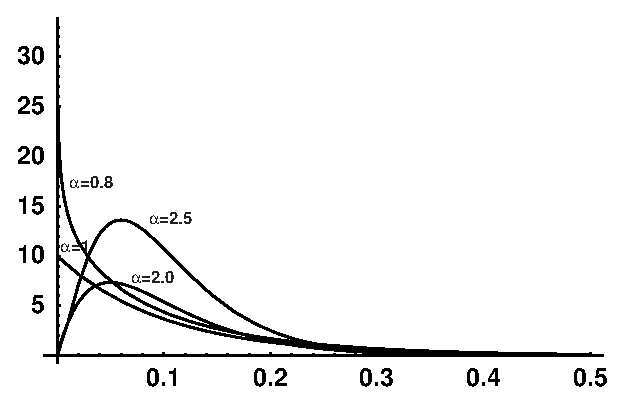
\includegraphics{gamma.eps}}
\end{center}
\caption{Examples of a gamma distribution.}\label{fig:asrv}
\end{figure}

The mean substitution rate in each curve above is 0.1. The curves
differ only in the value of a parameter, $\alpha$, called the ``shape
parameter.'' The shape parameter gives a nice numerical description of
how much rate variation there is, except that it's backwards. The
larger the parameter, the less among-site rate variation
there~is.\index{among-site rate variation!shape parameter}

\section*{The neutral theory of molecular evolution}

I didn't make a big deal of it in what we just went over, but in
deriving the Jukes-Cantor equation I used the phrase ``substitution
rate'' instead of the phrase ``mutation rate.''\footnote{In fact, I
  just mentioned the distinction in passing in two different
  footnotes.} As a preface to what is about to follow, let me explain
the difference.\index{mutation rate}\index{substitution rate}

\begin{itemize}

\item {\it Mutation rate\/} refers to the rate at which changes are
  incorporated into a nucleotide sequence during the process of
  replication, i.e., the probability that an allele differs from the
  copy of that allele in its parent from which it was derived. {\it
    Mutation rate\/} refers to the rate at which mutations
  arise.\index{mutation rate}

\item An allele substitution occurs when a newly arisen allele is
  incorporated into a population, e.g., when a newly arisen allele
  becomes fixed in a population. {\it Substitution rate\/} refers to
  the rate at which allele substitutions occur.\index{substitution rate}

\end{itemize}

\noindent Mutation rates and substitution rates are obviously
related{\dash}substitutions can't happen unless mutations occur, after
all{\dash}, but it's important to remember that they refer to
different processes.

\section*{Early empirical observations}

By the early 1960s amino acid sequences of hemoglobins and cytochrome
{\it c\/} for many mammals had been determined. When the sequences
were compared, investigators began to notice that the number of amino
acid differences between different pairs of mammals seemed to be
roughly proportional to the time since they had diverged from one
another, as inferred from the fossil record. Zuckerkandl and
Pauling~\cite{Zuckerkandl-Pauling65} proposed the {\it molecular clock
hypothesis\/} to explain these results. Specifically, they proposed
that there was a constant rate of amino acid substitution over
time. Sarich and Wilson~\cite{Sarich-Wilson67,Wilson-Sarich69} used
the molecular clock hypothesis to propose that humans and apes
diverged approximately 5 million years ago. While that proposal may
not seem particularly controversial now, it generated enormous
controversy at the time, because at the time many paleoanthropologists
interpreted the evidence to indicate humans diverged from apes as much
as 30 million years ago.\index{molecular clock}

One year after Zuckerkandl and Pauling's paper, Harris~\cite{Harris66}
and Hubby and Lewontin~\cite{Hubby-Lewontin66,Lewontin-Hubby66} showed
that protein electrophoresis could be used to reveal surprising
amounts of genetic variability within populations. Harris studied
10 loci in human populations, found three of them to be polymorphic,
and identified one locus with three alleles. Hubby and Lewontin
studied 18 loci in {\it Drosophila pseudoobscura\/}, found seven to be
polymorphic, and five that had three or more alleles.

Both sets of observations posed real challenges for evolutionary
geneticists. It was difficult to imagine an evolutionary mechanism
that could produce a constant rate of substitution. It was similarly
difficult to imagine that natural selection could maintain so much
polymorphism within populations. The ``cost of selection,'' as
Haldane~\cite{Haldane-1957} called it would simply be too
high.\index{cost of selection}

\section*{Neutral substitutions and neutral variation}

Kimura~\cite{Kimura68} and King and Jukes~\cite{King-Jukes69} proposed
a way to solve both empirical problems. If the vast majority of amino
acid substitutions are selectively neutral,\footnote{Notice that I
  just said that we're going to assume that the vast majority of
  nucleotide {\it substitutions\/} are selectively neutral. This
  doesn't mean that most nucleotide {\it mutations\/} are selectively
  neutral. Indeed, we'll see that most of them are deleterious.} then
substitutions will occur at approximately a constant rate~(assuming
that substitution rates don't vary over time) and it will be easy to
maintain lots of polymorphism within populations because there will be
no cost of selection. I'll develop both of those points in a bit more
detail in just a moment, but let me first be precise about what the
neutral theory of molecular evolution actually proposes. More
specifically, let me first be precise about what it does {\it not\/}
propose. I'll do so specifically in the context of protein evolution
for now, although we'll broaden the scope later.

\begin{itemize}

\item {\it The neutral theory asserts that alternative alleles at
    variable protein loci are selectively neutral.} This does {\it
    not\/} mean that the locus is unimportant, only that the
  alternative alleles found at this locus are selectively
  neutral.\index{neutral alleles}

\begin{itemize}

\item Glucose-phosphate isomerase is an esssential enzyme. It
  catalyzes the first step of glycolysis, the conversion of
  glucose-6-phosphate into fructose-6-phosphate.

\item Natural populations of many, perhaps most, populations of plants
  and animals are polymorphic at this locus, i.e., they have two or
  more alleles with different amino acid sequences.

\item The neutral theory asserts that the alternative alleles are
  essentially equivalent in fitness, in the sense that genetic drift,
  rather than natural selection, dominates the dynamics of frequency
  changes among them.

\end{itemize}

\item By {\it selectively neutral\/} we do {\it not\/} mean that the
  alternative alleles have no effect on physiology or fitness. We mean
  that the selection among different genotypes at this locus is
  sufficiently weak that the pattern of variation is determined by the
  interaction of mutation, drift, mating system, and migration. This
  is roughly equivalent to saying that $N_es < 1$, where $N_e$ is the
  effective population size and $s$ is the selection coefficient on
  alleles at this locus.\index{selective neutrality}

\begin{itemize}

\item Experiments in {\it Colias\/} butterflies, and other organisms
  have shown that different electrophoretic variants of GPI have
  different enzymatic capabilities and different thermal
  stabilities. In some cases, these differences have been related to
  differences in individual performance.

\item If populations of {\it Colias\/} are large and the differences
  in fitness associated with differences in genotype are large, i.e.,
  if $N_es > 1$, then selection plays a predominant role in
  determining patterns of diversity at this locus, i.e., the neutral
  theory of molecular evolution would not apply.

\item If populations of {\it Colias\/} are small or the differences in
  fitness associated with differences in genotype are small, or both,
  then drift plays a predominant role in determining patterns of
  diversity at this locus, i.e., the neutral theory of molecular
  evolution applies.

\end{itemize}

\end{itemize}

\noindent In short, the neutral theory of molecular really asserts
only that observed amino acid substitutions and polymorphisms are {\it
effectively\/} neutral, not that the loci involved are unimportant or
that allelic differences at those loci have no effect on
fitness.\index{neutral theory!effective neutrality}\index{effective neutrality}

\subsection*{The rate of molecular evolution}

We're now going to calculate the rate of molecular evolution, i.e.,
the rate of allelic substitution, under the hypothesis that mutations
are selectively neutral.\footnote{Notice that contrary to what I said
  earlier, here I am assuming that {\it mutations\/} are neutral, not
  just substitutions.} To get that rate we need two things: the rate
at which new mutations occur and the probability with which new
mutations are fixed. In a word equation\index{molecular
  clock!derivation}
\begin{eqnarray*}
\mbox{\# of substitutions/generation} &=& (\mbox{\# of mutations/generation})\times(\mbox{probability
  of fixation}) \\
\lambda &=& \mu_0p_0 \quad .
\end{eqnarray*}
Surprisingly,\footnote{Or perhaps not.} it's pretty easy to calculate
both $\mu_0$ and $p_0$ from first principles.

In a diploid population of size $N$, there are $2N$ gametes. The
probability that any one of them mutates is just the mutation rate,
$\mu$, so
\begin{equation}
\mu_0 = 2N\mu \quad . \label{eq:mu-0}
\end{equation}
To calculate the probability of fixation, we have to say something
about the dynamics of alleles in populations. Let's suppose that we're
dealing with a single population, to keep things simple. Now, you have
to remember a little of what you learned about the properties of
genetic drift. If the current frequency of an allele is $p_0$, what's
the probability that is eventually fixed?  $p_0$. When a new mutation
occurs there's only one copy of it,\footnote{By definition. It's new.}
so the frequency of a newly arisen mutation is $1/2N$ and
\begin{equation}
p_0 = \frac{1}{2N} \quad . \label{eq:p-0}
\end{equation}
Putting~(\ref{eq:mu-0}) and~(\ref{eq:p-0}) together we find
\begin{eqnarray*}
\lambda &=& \mu_0p_0 \\
        &=& (2N\mu)\left(\frac{1}{2N}\right) \\
        &=& \mu \quad .
\end{eqnarray*}
In other words, if mutations are selectively neutral, the substitution
rate is equal to the mutation rate. Since mutation rates are (mostly)
governed by physical factors that remain relatively constant, mutation
rates should remain constant, implying that substitution rates should
remain constant if substitutions are selectively neutral. In short, if
mutations are selectively neutral, we expect a molecular
clock.\index{molecular clock}

\subsection*{Diversity in populations}

Protein-coding genes consist of hundreds or thousands of nucleotides,
each of which could mutate to one of three other
nucleotides.\footnote{Why three when there are four nucleotides?
  Because if the nucleotide at a certain position is an A, for
  example, it can only {\it change\/} to a C, G, or T.} That's not an
infinite number of possibilities, but it's pretty large.\footnote{If a
  protein consists of 400 amino acids, that's 1200 nucleotides. There
  are $4^{1200} \approx 10^{720}$ different sequences that are 1200
  nucleotides long. For context, there are only about
  $3.28 \times 10^{80}$ elementary particles in the
  universe~(\url{https://www.popularmechanics.com/space/a27259/how-many-particles-are-in-the-entire-universe/}).}
It suggests that we could treat every mutation that occurs as if it
were completely new, a mutation that has never been seen before and
will never be seen again. Does that description ring any bells? Does
the infinite alleles model sound familiar? It should, because it
exactly fits the situation I've just
described.\index{mutation!infinite alleles model}

Having remembered that this situation is well described by the
infinite alleles model, I'm sure you'll also remember that we can
calculate the equilibrium inbreeding coefficient for the infinite
alleles model, i.e.,
\[
f = \frac{1}{4N_e\mu + 1} \quad .
\]
What's important about this for our purposes, is that to the extent
that the infinite alleles model is appropriate for molecular data,
then $f$ is the frequency of homozygotes we should see in populations
and $1-f$ is the frequency of heterozygotes. So in large populations
we should find more diversity than in small ones, which is roughly
what we do find. Notice, however, that here we're talking about
heterozygosity at individual nucleotide positions,\footnote{Since the
  mutation rate we're talking about applies to individual nucleotide
  positions.} not heterozygosity of halpotypes.

\section*{Conclusions}

In broad outline then, the neutral theory does a pretty good job of
dealing with at least some types of molecular data. I'm sure that some
of you are already thinking, ``But what about third codon positions
{\it versus\/} first and second?'' or ``What about the observation
that histone loci evolve much more slowly than interferons or MHC
loci?''  Those are good questions, and those are where we're going
next. As we'll see, molecular evolutionists have elaborated the
framework extensively\footnote{That mean's they've made it more
  complicated.} in the last fifty years, but these basic principles
underlie every investigation that's conducted. That's why I wanted to
spend a fair amount of time going over the logic and
consequences. Besides, it's a rare case in population genetics where
the fundamental mathematics that lies behind some important
predictions are easy to understand.\footnote{It's the concepts that
  get tricky, not the algebra, or at least that's what I think.}

\bibliography{popgen}
\bibliographystyle{plain}

\ccLicense

\end{document}



\documentclass[12pt]{article}
\usepackage{lecture}
\usepackage{graphics}
\usepackage{html}
\usepackage{url}

\newcommand{\copyrightYears}{2001-2021}

\title{Patterns of nucleotide and amino acid substitution}

\begin{document}

\maketitle

\thispagestyle{first}

\section*{Introduction}

So, I've just suggested that the neutral theory of molecular evolution
explains quite a bit, but it also ignores quite a bit. The derivations
we did assumed that all substitutions are equally likely to occur,
because they are selectively neutral. That isn't plausible. We need
look no further than sickle cell anemia to see an example of a protein
polymorphism in which a single nucleotide substitution and a single
amino acid difference has a very large effect on fitness. Even
reasoning from first principles we can see that it doesn't make much
sense to think that all nucleotide substitutions are created
equal. Just as it's unlikely that you'll improve the performance of
your car if you pick up a sledgehammer, open its hood, close your
eyes, and hit something inside, so it's unlikely that picking a random
amino acid in a protein and substituting it with a different one will
improve the function of the protein.\footnote{Obviously it happens
  sometimes. If it didn't, there wouldn't be any adaptive
  evolution. It's just that, on average, mutations are more likely to
  decrease fitness than to increase it. }\index{sledgehammer
  principle}

\section*{The genetic code}

Of course, not all nucleotide sequence substitutions lead to amino
acid substitutions in protein-coding genes. There is redundancy in the
genetic code. Table~\ref{table:code} is a list of the codons in the
universal genetic code.\footnote{By the way, the ``universal'' genetic
  code is not universal. There are at least
  31~(\url{https://www.ncbi.nlm.nih.gov/Taxonomy/Utils/wprintgc.cgi}),
  but all of them have similar redundancy properties.} Notice that
there are only two amino acids, methionine and tryptophan, that have a
single codon. All the rest have at least two. Serine, arginine, and
leucine have six.\index{genetic code}

\begin{table}
\begin{center}
\begin{tabular}{llllllll}
\hline\hline
      & Amino &       & Amino &       & Amino &       & Amino \\
Codon & Acid  & Codon & Acid  & Codon & Acid  & Codon & Acid \\
\hline
UUU   & Phe   & UCU   & Ser   & UAU   & Tyr   & UGU   & Cys \\
UUC   & Phe   & UCC   & Ser   & UAC   & Tyr   & UGC   & Cys \\
UUA   & Leu   & UCA   & Ser   & UAA   & Stop  & UGA   & Stop \\
UUG   & Leu   & UCG   & Ser   & UAG   & Stop  & UGG   & Trp \\
      &       &       &       &       &       &       & \\
CUU   & Leu   & CCU   & Pro   & CAU   & His   & CGU   & Arg \\
CUC   & Leu   & CCC   & Pro   & CAC   & His   & CGC   & Arg \\
CUA   & Leu   & CCA   & Pro   & CAA   & Gln   & CGA   & Arg \\
CUG   & Leu   & CCG   & Pro   & CAG   & Gln   & CGG   & Arg \\
      &       &       &       &       &       &       & \\
AUU   & Ile   & ACU   & Thr   & AAU   & Asn   & AGU   & Ser \\
AUC   & Ile   & ACC   & Thr   & AAC   & Asn   & AGC   & Ser \\
AUA   & Ile   & ACA   & Thr   & AAA   & Lys   & AGA   & Arg \\
AUG   & Met   & ACG   & Thr   & AAG   & Lys   & AGG   & Arg \\
      &       &       &       &       &       &       & \\
GUU   & Val   & GCU   & Ala   & GAU   & Asp   & GGU   & Gly \\
GUC   & Val   & GCC   & Ala   & GAC   & Asp   & GGC   & Gly \\
GUA   & Val   & GCA   & Ala   & GAA   & Glu   & GGA   & Gly \\
GUG   & Val   & GCG   & Ala   & GAG   & Glu   & GGG   & Gly \\
\hline
\end{tabular}
\end{center}
\caption{The universal genetic code.}\label{table:code}
\end{table}

Moreover, most of the redundancy is in the third position, where we
can distinguish 2-fold from 4-fold redundant
sites~(Table~\ref{table:fold}). 2-fold redundant sites are those at
which either one of two nucleotides can be present in a codon for a
single amino acid. 4-fold redundant sites are those at which any of
the four nucleotides can be present in a codon for a single amino
acid. In some cases, there is redundancy in the first codon position,
e.g, both AGA and CGA are codons for arginine. Thus, many nucleotide
substitutions at third positions do not lead to amino acid
substitutions, and some nucleotide substitutions at first positions do
not lead to amino acid substitutions. But every nucleotide
substitution at a second codon position leads to an amino acid
substitution. Nucleotide substitutions that do not lead to amino acid
substitutions are referred to as {\it synonymous substitutions},
because the codons involved are synonymous, i.e., code for the same
amino acid. Nucleotide substitutions that do lead to amino acid
substitutions are {\it non-synonymous substitutions}.\index{genetic code!redundancy}\index{synonymous substitutions}\index{non-synonymous substitutions}

\begin{table}
\begin{center}
\begin{tabular}{lll}
\hline\hline
      & Amino & \\
Codon & Acid  & Redundancy \\
\hline
CCU   & Pro   & 4-fold \\
CCC \\
CCA \\
CCG \\
\hline
AAU   & Asn   & 2-fold \\
AAC \\
AAA   & Lys   & 2-fold \\
AAG \\
\hline
\end{tabular}
\end{center}
\caption{Examples of 4-fold and 2-fold redundancy in the 3rd position
  of the universal genetic code.}\label{table:fold}
\end{table}

\section*{Rates of synonymous and non-synonymous substitution}

By using a modification of the simple Jukes-Cantor model we
encountered before, it is possible to make separate estimates of the
number of synonymous substitutions and of the number of non-synonymous
substitutions that have occurred since two sequences diverged from a
common ancestor. If we combine an estimate of the {\it number\/} of
differences with an estimate of the {\it time of divergence\/} we can
estimate the rates of synonymous and non-synonymous
substitution~(number/time). Table~\ref{table:substitution-data} shows
some representative estimates for the rates of synonymous and
non-synonymous substitution in different genes studied in
mammals.\index{substitution rate}

\begin{table}
\begin{center}
\begin{tabular}{lcc}
\hline\hline
Locus     & Non-synonymous rate & Synonymous rate \\
\hline
Histone \\
\quad H4  & 0.00                & 3.94 \\
\quad H2  & 0.00                & 4.52 \\
Ribosomal proteins \\
\quad S17 & 0.06                & 2.69 \\
\quad S14 & 0.02                & 2.16 \\
Hemoglobins \& myoglobin \\
\quad $\alpha$-globin & 0.56    & 4.38 \\
\quad $\beta$-globin  & 0.78    & 2.58 \\
\quad Myoglobin       & 0.57    & 4.10 \\
Interferons \\
\quad $\gamma$  & 3.06          & 5.50 \\
\quad $\alpha$1 & 1.47          & 3.24 \\
\quad $\beta$1  & 2.38          & 5.33 \\
\hline
\end{tabular}
\end{center}
\caption{Representative rates of synonymous and non-synonymous
  substitution in mammalian genes~(from~\cite{Li97}). Rates are
  expressed as the number of substitutions per $10^9$
  years.}\label{table:substitution-data}
\end{table}

Two very important observations emerge after you've looked at this
table for awhile. The first won't come as any shock. The rate of
non-synonymous substitution is generally lower than the rate of
synonymous substitution. This is a result of the ``sledgehammer
principle'' I mentioned earlier. Just as taking a sledgehammer to your
car engine and making random changes is unlikely to make it run
better, so making random changes to the amino acid composition of a
protein is unlikely to make it function better. Mutations that change
the amino acid sequence of a protein are more likely to reduce that
protein's functionality than to increase it. As a result, they are
likely to lower the fitness of individuals carrying them, and they
will have a lower probability of being fixed than those mutations that
do not change the amino acid sequence.\index{sledgehammer principle}\footnote{Remember 
our discussion of the probability that disfavored mutations are fixed
as a result of natural selection. They can be fixed, but they are less
likely to be fixed than those that are neutral.}
  
The second observation is more subtle. Rates of non-synonymous
substitution vary by more than two orders of magnitude: 0.02
substitutions per nucleotide per billion years in ribosomal protein
S14 to 3.06 substitutions per nucleotide per billion years in
$\gamma$-interferon, while rates of synonymous substitution vary only
by a factor of two (2.16 in ribosomal protein S14 to 5.50 in $\gamma$
interferons. If synonymous substitutions are neutral, as they probably
are to a first approximation,\footnote{We'll see that they may not be
  completely neutral a little later, but at least it's reasonable to
  believe that the intensity of selection to which they are subject is
  a lot less than that to which non-synonymous substitutions are
  subject.}  then the rate of synonymous substitution should equal the
mutation rate. Thus, the rate of synonymous substitution should be
approximately the same at every locus, which is roughly what we
observe. But proteins differ in the degree to which their
physiological function affects the performance and fitness of the
organisms that carry them. Some, like histones and ribosomal proteins,
are intimately involved with chromatin or translation of messenger RNA
into protein. It's easy to imagine that just about any change in the
amino acid sequence of such proteins will have a detrimental effect on
their function. Others, like interferons, are involved in responses to
viral or bacterial pathogens. It's easy to imagine not only that the
selection on these proteins might be less intense, but that some amino
acid substitutions might actually be favored by natural selection
because they enhance resistance to certain strains of pathogens. Thus,
the probability that a non-synonymous substitution will be fixed is
likely to vary substantially among genes, just as we observe.

\section*{Revising the neutral theory}

So we've now produced empirical evidence that many mutations are {\it
  not\/} neutral. Does this mean that we throw the neutral theory of
molecular evolution away? Hardly. We need only modify it a little to
accommodate these new observations.\index{neutral theory!modifications}

\begin{itemize}

\item {\it Most non-synonymous substitutions are deleterious.\/} We
  can actually generalize this assertion a bit and say that most
  mutations that affect function are deleterious. After all, organisms
  have been evolving for about 3.5 billion years. Wouldn't you expect
  their cellular machinery to work pretty well by now?

\item {\it Most molecular variability found in natural populations is
    selectively neutral.} If most function-altering mutations are
  deleterious, it follows that we are unlikely to find much variation
  in populations for such mutations. Selection will quickly eliminate
  them.\footnote{Remember, when I say that ``the variability is
    selectively neutral,'' that's shorthand for saying that ``the
    product of effective population size and the selection coefficient
    on different alleles is less than one, meaning that the dynamics
    of allele frequency change are more similar to those of an allele
    that has no effects on fitness than to those of an allele with an
    effect on fitness when we can neglect genetic drift.''}

\item {\it Natural selection is primarily purifying.} Although natural
  selection for variants that improve function is ultimately the
  source of adaptation, even at the molecular level, most of the time
  selection is simply eliminating variants that are less fit than the
  norm, not promoting the fixation of new variants that increase
  fitness.

\item {\it Alleles enhancing fitness are rapidly
    incorporated.}\footnote{To be more precise I should have written
    {\it Alleles enhancing fitness are rapidly incorporated, {\bf when
        they are not lost quickly as a result of genetic drift}.\/}}
  They do not remain polymorphic for long, so we aren't likely to find
  them when they're polymorphic.

\end{itemize}

As we'll see, even these revisions aren't entirely sufficient, but
what we do from here on out is more to provide refinements and
clarifications than to undertake wholesale revisions.

\bibliography{popgen}
\bibliographystyle{plain}

\ccLicense

\end{document}



\documentclass[12pt]{article}
\usepackage{lecture}
\usepackage{graphicx}
\usepackage{epstopdf}
\usepackage{html}
\usepackage{url}

\newcommand{\copyrightYears}{2001-2021}

\title{Detecting selection on nucleotide polymorphisms}

\begin{document}

\maketitle

\thispagestyle{first}

\section*{Introduction}

At this point, we've refined the neutral theory quite a bit. Our
understanding of how molecules evolve now recognizes that some
substitutions are more likely than others, but we're still proceeding
under the assumption that most nucleotide substitutions are neutral or
detrimental. So far we've argued that variation like what Hubby and
Lewontin~\cite{Hubby-Lewontin66,Lewontin-Hubby66} found is not likely
to be maintained by natural selection. But we have strong evidence
that heterozygotes for the sickle-cell allele are more fit than either
homozygote in human populations where malaria is prevalent. That's an
example where selection is acting to maintain a polymorphism, not to
eliminate it. Are there other examples? How could we detect them?

In the 1970s a variety of studies suggested that a polymorphism in the
locus coding for alcohol dehydrogenase in {\it Drosophila
  melanogaster\/} might not only be subject to selection but that
selection may be acting to maintain the polymorphism. As DNA
sequencing became more practical at about the same time,\footnote{It
  was still {\it vastly\/} more laborious than it is now.} population
geneticists began to realize that comparative analyses of DNA
sequences at protein-coding loci could provide a powerful tool for
unraveling the action of natural selection. Synonymous sites within a
protein-coding sequence provide a powerful standard of
comparision. Regardless of

\begin{itemize}

\item the demographic history of the population from which the
  sequences were collected,

\item the length of time that populations have been evolving under the
  sample conditions and whether it has been long enough for the
  population to have reached a drift-migration-mutation-selection
  equilibrium, or

\item the actual magnitude of the mutation rate, the migration rate,
  or the selection coefficients

\end{itemize}

\noindent the synonymous positions within the sequence provide an
internal control on the amount and pattern of differentiation that
should be expected when substitutions are neutral.\footnote{Ignoring,
  for the moment, the possibility that there may be selection on codon
  usage.}  Thus, if we see different patterns of nucleotide
substitution at synonymous and non-synonymous sites, we can infer that
selection is having an effect on amino acid substitutions.

\section*{Nucleotide sequence variation at the {\it Adh\/} locus in
  {\it Drosophila melanogaster}}\index{Drosophila@\textit{Drosophila}!\textit{melanogaster}}\index{alcohol dehydrogenase}\index{Adh}

Kreitman~\cite{Kreitman83} took advantage of these ideas to provide
additional insight into whether natural selection was likely to be
involved in maintaining the polymorphism at {\it Adh\/} in {\it
  Drosophila melanogaster}. He cloned and sequenced 11 alleles at this
locus, each a little less than 2.4kb in length.\footnote{Think about
  how the technology has changed since then. This work represented a
  major part of his Ph.D. dissertation, and the results were published
  as an article in {\it Nature}. Now an undergraduate would do
  substantially more for an independent study project.} If we restrict
our attention to the coding region, a total of 765bp, there were 6
distinct sequences that differed from one another at between 1 and 13
sites. Given the observed level of polymorphism within the gene, there
should be 9 or 10 amino acid differences observed as well, but only
one of the nucleotide differences results in an amino acid difference,
the amino acid difference associated with the already recognized
electrophoretic polymorphsim. Thus, there is significantly less amino
acid diversity than expected if nucleotide substitutions were neutral,
consistent with my assertion that most mutations are deleterious and
that natural selection will tend to eliminate
them.\index{Adh!purifying selection} In other words, another example
of the ``sledgehammer principle.''\index{sledgehammer principle}

Does this settle the question? Is the {\it Adh\/} polymorphism another
example of allelic variants being neutral or selected against? Would I
be asking these questions if the answer were ``Yes''?

\subsection*{Kreitman and Aguad{\'e}}

A few years after Kreitman~\cite{Kreitman83} appeared, Kreitman and
Aguad{\'e}~\cite{Kreitman-Aguade86} published an analysis in which
they looked at levels of nucleotide diversity in the {\it Adh\/}
region, as revealed through analysis of RFLPs, in {\it
  D. melanogaster\/} and the closely related {\it D. simulans}. Why
the comparative approach? Well, Kreitman and Aguad{\'e} recognized
that the neutral theory of molecular evolution makes two predictions
that are related to the underlying mutation rate:

\begin{itemize}

\item If mutations are neutral, the substitution rate is equal to the
  mutation rate.

\item If mutations are neutral, the diversity within populations
  should be about $4N_e\mu/(4N_e\mu + 1)$.

\end{itemize}

\noindent Thus, if variation at the {\it Adh\/} locus in {\it
  D. melanogaster\/} is selectively neutral, the amount of divergence
between {\it D. melanogaster\/} and {\it D. simulans\/} should be
related to the amount of diversity within each. What they found
instead is summarized in Table~\ref{table:ka}.\index{Adh!balancing selection}\index{diversity-divergence}

The expected level of diversity in each part of the {\it Adh\/} locus
is calculated assuming that the probability of polymorphism is
independent of what position in the locus we are
examining.\footnote{It's important to note that what I've labeled as
  the {\it Adh\/} locus in Table~\ref{table:ka} is the region that
  contains the protein coding part of the locus. The 5' and 3'
  flanking regions are physically adjacent, but none of the
  nucleotides in these parts of the gene are translated into the {\it
    Adh\/} enzyme.} Specifically, Kreitman and Aguad{\'e} calculated
the expected polymorphism as follows:

\begin{itemize}

\item They calculated the number of ``site equivalents'' in each
  region of the locus. A site equivalent is the actual length of the
  region~(in number of nucleotides) times the fraction of changes
  within that sequence that would lead to gain or loss of a
  restriction site.\footnote{Because sequencing was extremely
    time-consuming in the mid-1980s, it was impractical to sequence
    the {\it Adh\/} locus in all of the 81 lines they used in the
    analysis. Instead they used restriction enzymes to reveal some of
    the nucleotide sequence variation in the locus.} There were 414
  site equivalents in the 5' flanking region, 411 site equivalents in
  the {\it Adh\/} locus, and 129 site equivalents in the 3' flanking
  region.

\item They calculated the fraction of site equivalents that were
  polymorphic across the entire locus:
\[
\frac{25}{414+411+129} \approx 0.026 \quad .
\]

\item They calculated the expected number of polymorphic sites within
  a region as the product of the number of site equivalents and the
  fraction of polymorphic site equivalents.

\end{itemize}

\noindent They used the same approach to calculate the expected
divergence between {\it D. melanogaster\/} and {\it D. simulans\/}
with one important exception. They directly compared the nucleotide
sequence of one {\it Adh\/} allele from {\it D. melanogaster\/} with
one {\it Adh\/} allele from {\it D. simulans}.\footnote{Can you
  explain why it's reasonable to estimate divergence between alleles
  in these species using only one allele from each of them?} As a
result, they didn't have to use the site equivalent correction. They
could directly use the number of nucleotides in each region of the
gene.

\begin{table}
\begin{center}
\begin{tabular}{l|ccc}
\hline\hline
         & 5' flanking & {\it Adh\/} locus & 3' flanking \\
\hline
Diversity$^1$ \\
\quad Observed & 9     & {\bf 14}   & 2    \\
\quad Expected & 10.8  & 10.8 & 3.4  \\
Divergence$^2$ \\
\quad Observed & 86    & 48   & 31   \\
\quad Expected & 55    & {\bf 76.9} & 33.1 \\
\hline
\multicolumn{4}{l}{$^1$Number of polymorphic sites within {\it
         D. melanogaster\/}} \\
\multicolumn{4}{l}{$^2$Number of nucleotide differences between {\it
         D. melanogaster\/} and {\it D. simulans}}
\end{tabular}
\end{center}
\caption{Diversity and divergence in the {\it Adh\/} region of {\it
    Drosophila}~(from~\cite{Kreitman-Aguade86}).}\label{table:ka}
\end{table}

Notice that there is substantially less divergence between {\it
  D. melanogaster\/} and {\it D. simulans\/} at the {\it Adh\/} locus
than would be expected, based on the average level of divergence
across the entire region. That's consistent with the earlier
observation that most amino acid substitutions are selected
against. On the other hand, there is {\it more\/} nucleotide diversity
within {\it D. melanogaster\/} than would be expected based on the
levels of diversity seen in across the entire region. What gives?

Time for a trip down memory lane. Remember something called
``coalescent theory?'' It told us that for a sample of neutral genes
from a population, the expected time back to a common ancestor for all
of them is about $4N_e$ for a nuclear gene in a diploid
population. That means there's been about $4N_e$ generations for
mutations to occur. Suppose, however, that the electrophoretic
polymorphism were being maintained by natural selection. Then we might
well expect that it would be maintained for a lot longer than $4N_e$
generations. If so, there would be a lot more time for diversity to
accumulate. Thus, the excess diversity could be accounted for if there
is balancing selection at ADH.\index{coalescent!balancing selection}

\subsection*{Kreitman and Hudson}

Kreitman and Hudson~\cite{Kreitman-Hudson91} extended this approach by
looking more carefully within the region to see where they could find
differences between observed and expected levels of nucleotide
sequence diversity. They used a ``sliding window'' of 100 silent base
pairs in their calculations. By ``sliding window'' what they mean is
that first they calculate statistics for bases 1-100, then for bases
2-101, then for bases 3-102, and so on until they hit the end of the
sequence~(Figure~\ref{fig:kh}).

\begin{figure}
\begin{center}
\resizebox{!}{7cm}{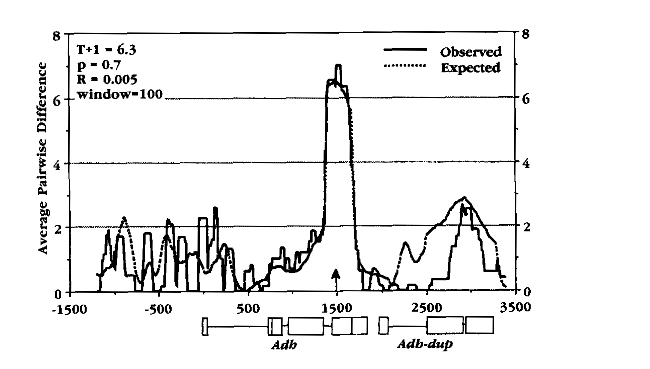
\includegraphics{kreitman-hudson.eps}}
\end{center}
\caption{Sliding window analysis of nucleotide diversity in the {\it
    Adh\/}-{\it Adh-dup} region of {\it Drosophila melanogaster}. The
  arrow marks the position of the single nucleotide substitution that
  distinguishes {\it Adh-F\/} from {\it
    Adh-S\/}~(from~\cite{Kreitman-Hudson91})}\label{fig:kh}
\end{figure}

To me there are two particularly striking things about this
figure. First, the position of the single nucleotide substitution
responsible for the electrophoretic polymorphism is clearly
evident. Second, the excess of polymorphism extends for only a 200-300
nucleotides in each direction. That means that the rate of
recombination {\it within\/} the gene is high enough to randomize the
nucleotide sequence variation farther away.\footnote{Remember this
  observation when we get to association mapping at the end of the
  course. In organisms with a large effective population size,
  associations due to physical linkage may fall off {\it very\/}
  rapidly, meaning that you would have to have a {\it very\/} dense
  map to have a hope of finding associations.}

\section*{Detecting selection in the human genome}

I've already mentioned the HapMap project~\cite{HapMap-2007}, a
collection of genotype data at roughly 3.2M SNPs in the human
genome. The data in phase II of the project were collected from four
populations:

\begin{itemize}

\item Yoruba (Ibadan, Nigeria)

\item Japanese (Tokyo, Japan)

\item Han Chinese (Beijing, China)

\item ancestry from northern and western Europe (Utah, USA)

\end{itemize}

We expect genetic drift to result in allele frequency differences
among populations, and we can summarize the extent of that
differentiation at each locus with $F_{ST}$. If all HapMap SNPs are
selectively neutral,\footnote{And unlinked to sites that are under
  selection.} then all loci should have the same $F_{ST}$ within the
bounds of statistical sampling error and the evolutionary sampling due
to genetic drift. A scan of human chromosome 7 reveals both a lot of
variation in individual-locus estimates of $F_{ST}$ and a number of
loci where there is substantially more differentiation among
populations than is expected by
chance~(Figure~\ref{fig:low-res-SNP}). At very fine genomic scales we
can detect even more outliers~(Figure~\ref{fig:high-res-SNP}),
suggesting that human populations have been subject to divergent
selection pressures at many different loci~\cite{Guo-etal-2009}.\index{F-statistics@$F$-statistics!outliers}

\begin{figure}
\begin{center}
\resizebox{\textwidth}{!}{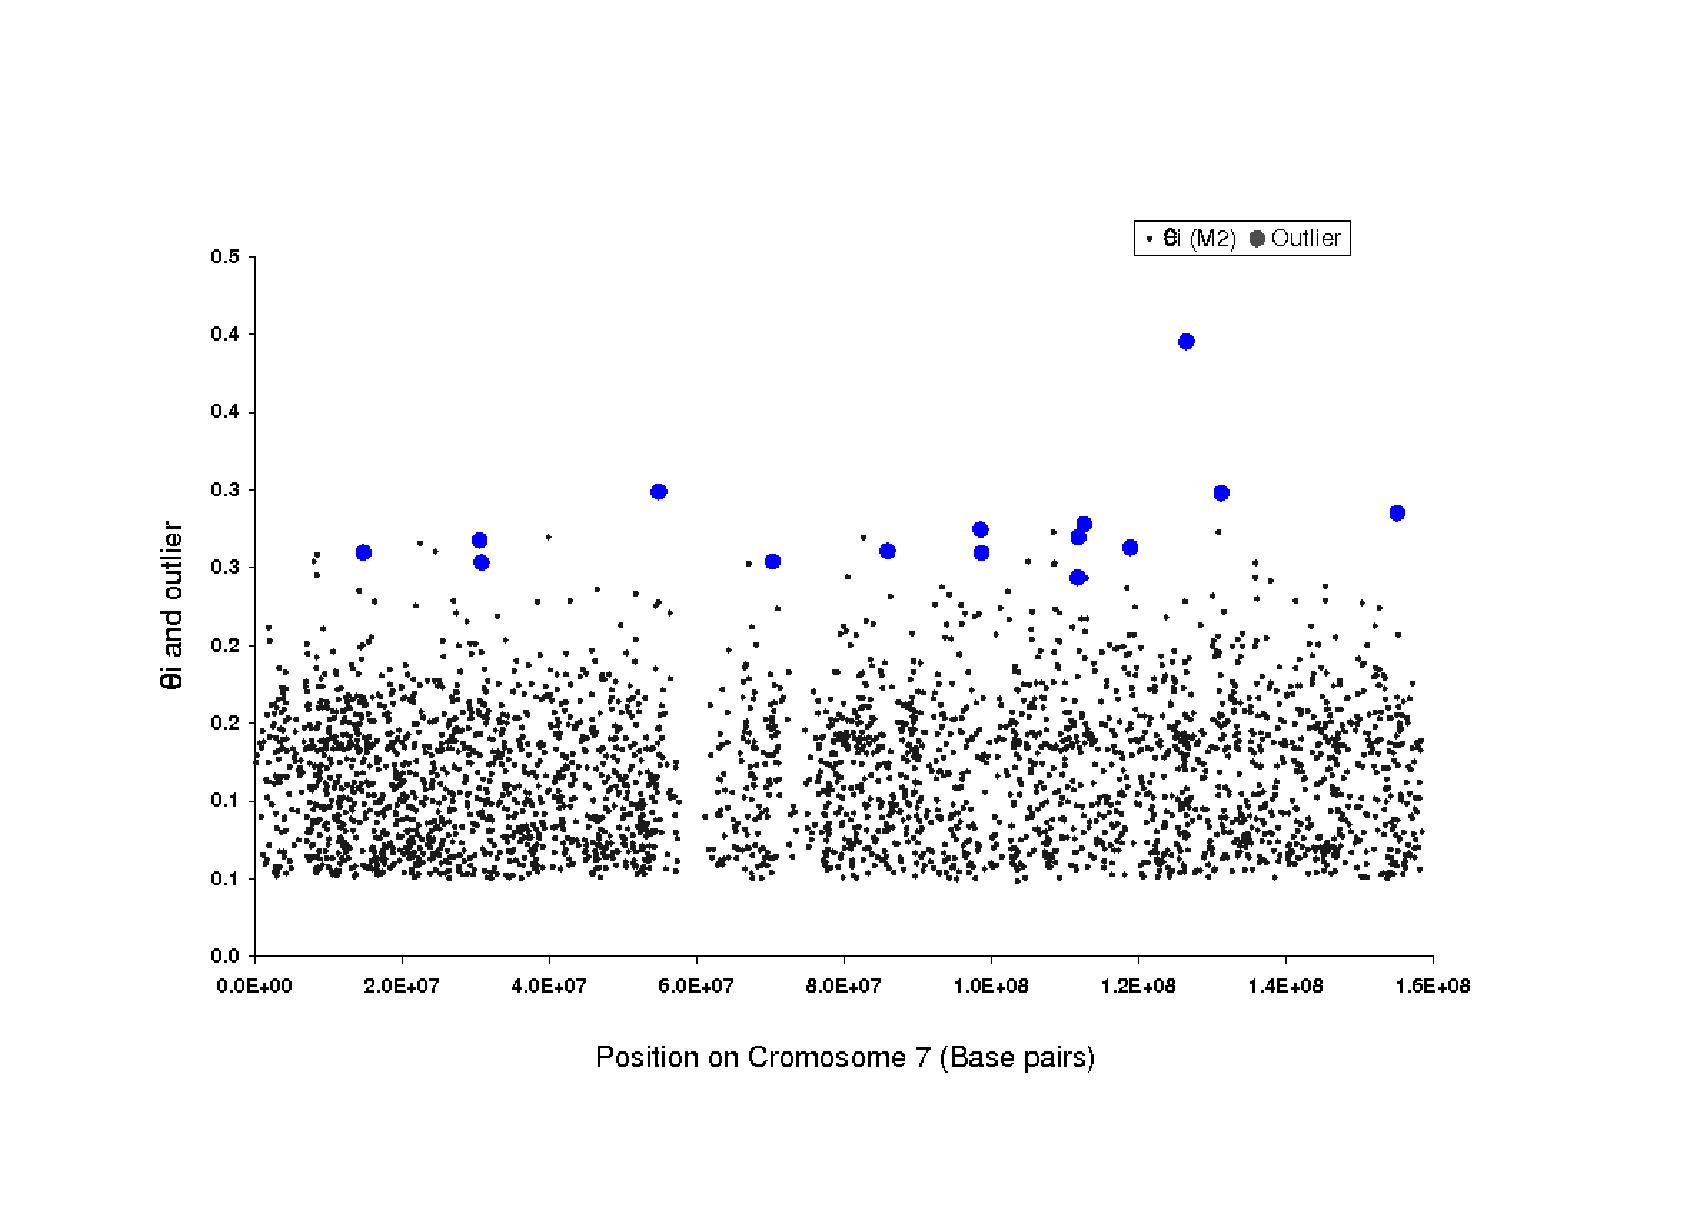
\includegraphics{outlier.eps}}
\end{center}
\caption{Single-locus estimates of $F_{ST}$ along chromosome 7 in the
  HapMap data set. Blue dots denote outliers. Adjacent SNPs in this
  sample are separated, on average, by about
  52kb. (from~\cite{Guo-etal-2009})}\label{fig:low-res-SNP}
\end{figure}

\begin{figure}
\begin{center}
\resizebox{0.7\textwidth}{!}{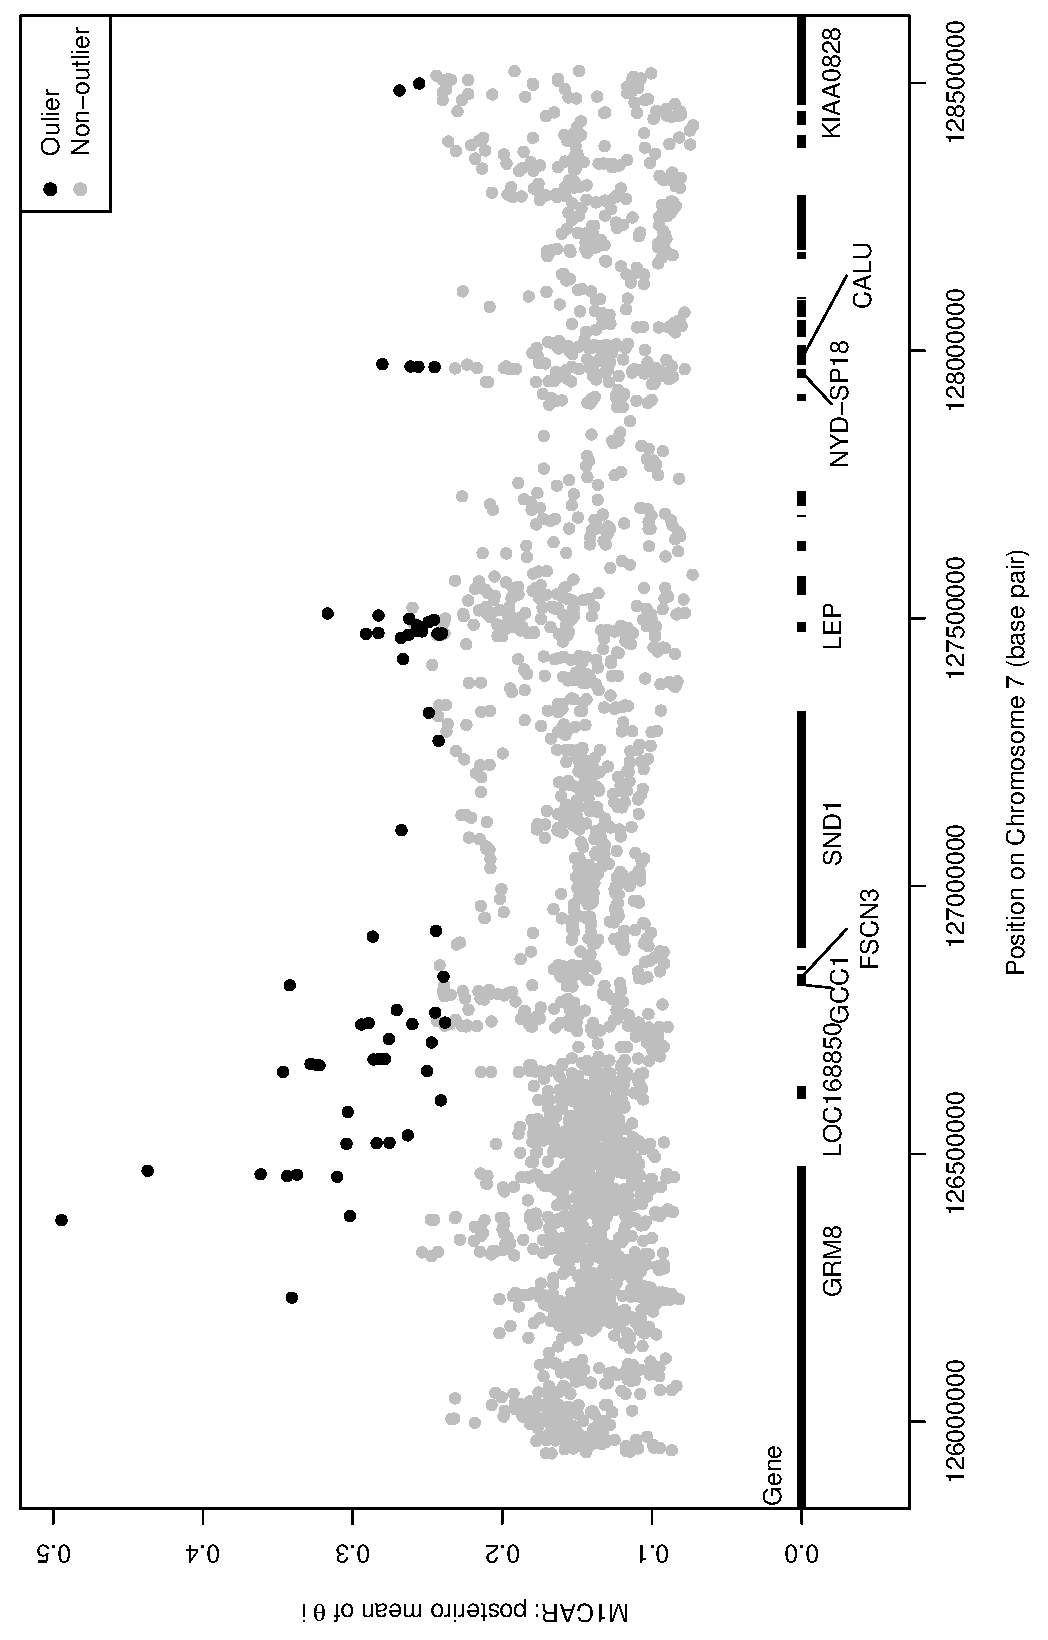
\includegraphics[angle=270]{outlier-high.eps}}
\end{center}
\caption{Single-locus estimates of $F_{ST}$ along a portion of
  chromosome 7 in the HapMap data set. Black dots denote
  outliers. Solid bars refert to previously identified genes. Adjacent
  SNPs in this sample are separated, on average, by about
  1kb. (from~\cite{Guo-etal-2009})}\label{fig:high-res-SNP}
\end{figure}

\section*{Tajima's $D$}\index{Tajima's $D$}

So far we've been comparing rates of synonymous and non-synonymous
substitution to detect the effects of natural selection on molecular
polymorphisms. Tajima~\cite{Tajima89} proposed a method that builds on
the foundation of the neutral theory of molecular evolution in a
different way. I've already mentioned the infinite alleles model of
mutation several times. When thinking about DNA sequences a closely
related approximation is to imagine that every time a mutation occurs,
it occurs at a different site.\footnote{Of course, we know this isn't
  true. Multiple substitutions {\it can\/} occur at any site. That's
  why the percent difference between two sequences isn't equal to the
  number of substitutions that have happened at any particular
  site. We're simply assuming that the sequences we're comparing are
  closely enough related that nearly all mutations have occurred at
  different positions.} If we do that, we have an {\it infinite
  sites\/} model of mutation.\index{mutation!infinite sites model}

When dealing with nucleotide sequences in a population context there
are two statistics of potential interest:

\begin{itemize}

\item The {\it number\/} of nucleotide positions at which a
  polymorphism is found or, equivalently, the number of segregating
  sites, $k$.\index{segregating sites}

\item The average number of nucleotide differences between two
  sequences, $\pi$, where $\pi$ is estimated as\index{nucleotide diversity}
\[
\pi = \sum x_ix_j\delta_{ij} \quad .
\]
In this expression, $x_i$ is the frequency of the $i$th haplotype and
$\delta_{ij}$ is the number of nucleotide sequence differences between
haplotypes $i$ and $j$.\footnote{I lied, but you must be getting used
  to that by now. This isn't quite the way you estimate it. To get an
  unbiased estimate of $\pi$, you have to multiply this equation by
  $n/(n-1)$, where $n$ is the number of haplotypes in your
  sample. And, of course, if you're Bayesian you'll be even a little
  more careful. You'll estimate $x_i$ using an appropriate prior on
  haplotype frequencies and you'll estimate the probability that
  haplotypes $i$ and $j$ are different at a randomly chosen position
  given the observed number of differences and the sequence length and
  multiply that probability by the sequence length giving you the
  expected number of differences between those two haplotypes. The
  expected number of differences will be close $\delta_{ij}$, but it
  won't be identical and it won't be a single number.}

\end{itemize}

The quantity $4N_e\mu$ comes up a lot in mathematical analyses of
molecular evolution. Population geneticists, being a lazy bunch, get
tired of writing that down all the time, so they invented the
parameter $\theta = 4N_e\mu$ to save themselves a little
time.\footnote{This is {\it not\/} the same $\theta$ we encountered
  when discussing $F$-statistics. Weir and Cockerham's $\theta$ is a
  different beast. I know it's confusing, but that's the way it
  is. When reading a paper, the context should make it clear which
  conception of $\theta$ is being used. Another thing to be careful of
  is that sometimes authors think of $\theta$ in terms of a haploid
  population. When they do, it's $2N_e\mu$. Usually the context makes
  it clear which definition is being used, but you have to remember to
  pay attention to be sure. If you follow population geneticists on
  Twitter, you'll often see them complaining about ``off by two''
  errors.} Under the infinite-sites model of DNA sequence evolution,
it can be shown that
\begin{eqnarray*}
\E(\pi) &=& \theta \\
\E(k) &=& \theta\sum_i^{n-1} \frac{1}{i} \quad ,
\end{eqnarray*}
where $n$ is the number of haplotypes in your sample.\footnote{The
  ``E'' refers to expectation. It is the average value of a random
  variable. $\mbox{E}(\pi)$ is read as ``the expectation of $\pi$.''}
This suggests that there are two ways to estimate $\theta$, namely
\begin{eqnarray*}
\hat \theta_\pi &=& \hat \pi \\
\hat \theta_k   &=& \frac{k}{\sum_i^{n-1}\frac{1}{i}} \quad ,
\end{eqnarray*}
where $\hat\pi$ is the average heterozygosity at nucleotide sites in
our sample and $k$ is the observed number of segregating sites in our
sample.\footnote{If your memory is really good, you may recognize that
  those estimates are method of moments estimates, i.e., parameter
  estimates obtained by equating sample statistics with their expected
  values.} If the nucleotide sequence variation among our haplotypes
is neutral and the population from which we sampled is in equilibrium
with respect to drift and mutation, then $\hat\theta_\pi$ and
$\hat\theta_k$ should be statistically indistinguishable from one
another. In other words,
\[
\hat D = \frac{\hat\theta_\pi -
  \hat\theta_k}{\mbox{Var}(\hat\theta_\pi - \hat\theta_k)} 
\]
should be indistinguishable from zero.\footnote{Dividing the
  difference between $\hat\theta_\pi$ and $\hat\theta_k$ by its
  variance makes the expectation of $\hat D$ zero and gives it a
  variance of one. This allows us to construct a statistical test of
  the difference between the observed $\hat D$ and the expectation if
  sequences are evolving neutrally and if the population is at a
  drift-mutation equilibrium. See~\cite{Tajima89} for details.} If it
is either negative or positive, we can infer that there's some
departure from the assumptions of neutrality and/or equilibrium. Thus,
$\hat D$ can be used as a test statistic to assess whether the data
are consistent with the population being at a neutral mutation-drift
equilibrium. Consider the value of $D$ under following
scenarios:\index{Tajima's $D$!interpretation}

\begin{description}

\item[Neutral variation] If the variation is neutral and the
  population is at a drift-mutation equilibrium, then $\hat D$ will be
  statistically indistinguishable from zero.

\item[Overdominant selection] Overdominance will allow alleles
  beloning to the different classes to become quite divergent from one
  another. $\delta_{ij}$ within each class will be small, but
  $\delta_{ij}$ between classes will be large and both classes will be
  in intermediate frequency, leading to large values of
  $\theta_\pi$. There won't be a similar tendency for the {\it
  number\/} of segregating sites to increase, so $\theta_k$ will be
  relatively unaffected. As a result, $\hat D$ will be positive.

\item[Population bottleneck] If the population has recently undergone
  a bottleneck, then $\pi$ will be little affected unless the
  bottleneck was prolonged and severe.\footnote{Why? Because most of
    the heterozygosity is due to alleles of moderate to high
    frequency, and those are not the ones likely to be lost in a
    bottleneck.}  $k$, however, may be substantially reduced. Thus,
  $\hat D$ should be positive.

\item[Purifying selection] If there is purifying selection, mutations
  will occur and accumulate at silent sites, but they aren't likely
  ever to become very common. Thus, there are likely to be lots of
  segregating sites, but not much heterozygosity, meaning that
  $\hat\theta_k$ will be large, $\hat\theta_\pi$ will be small, and
  $\hat D$ will be negative.

\item[Population expansion] Similarly, if the population has recently
  begun to expand, mutations that occur are unlikely to be lost,
  increasing $\hat\theta_k$, but it will take a long time before they
  contribute to heterozygosity, $\hat\theta_\pi$. Thus, $\hat D$ will
  be negative.

\end{description}

In short, $\hat D$ provides a different avenue for insight into the
evolutionary history of a particular nucleotide sequence. But
interpreting it can be a little tricky.

\begin{description}

\item[$\hat D = 0$:] We have no evidence for changes in population
  size or for any particular pattern of selection at the
  locus.\footnote{Please remember that the failure to detect a difference
    from 0 could mean that your sample size is too small to detect an
    important effect. If you can't detect a difference, you should try
    to assess what values of $D$ are consistent with your data and be
    appropriately circumspect in your conclusions.}

\item[$\hat D < 0$:] The population size may be increasing or we may
  have evidence for purifying selection at this locus.

\item[$\hat D > 0$:] The population may have suffered a recent
  bottleneck (or be decreaing) or we may have evidence for
  overdominant selection at this locus.

\end{description}

\noindent If we have data available for more than one locus, we may be
able to distinguish changes in population size from selection at any
particular locus. After all, all loci will experience the same
demographic effects, but we might expect selection to act differently
at different loci, especially if we choose to analyze loci with
different physiological function.

A quick search in Google Scholar reveals that the paper in which
Tajima described this approach~\cite{Tajima89} has been cited over
13,000
times.\footnote{\url{https://scholar.google.com/scholar?hl=en&as_sdt=0\%2C7&q=tajima+genetics+123\%3A585-595\%3B+1989&btnG=}
  Search on 30 July 2021.} Clearly it has been widely used for
interpreting patterns of nucleotide sequence variation. Although it is
a very useful statistic, Zeng et al.~\cite{Zeng-etal-2006} point out
that there are important aspects of the data that Tajima's $D$ does
not consider. As a result, it may be less powerful, i.e., less able to
detect departures from neutrality, than some alternatives.

\bibliography{popgen}
\bibliographystyle{plain}

\ccLicense

\end{document}




\part{Phylogeography}

\documentclass[12pt]{article}
\usepackage{lecture}
\usepackage{graphicx}
\usepackage{html}
\usepackage{url}
\usepackage{epstopdf}

\newcommand{\copyrightYears}{2001-2021}

\title{Analysis of molecular variance (AMOVA)}

\begin{document}

\maketitle

\thispagestyle{first}

\section*{Introduction}

We've already encountered $\pi$, the nucleotide diversity in a
population, namely
\[
\pi = \sum_{ij} x_ix_j \delta_{ij} \quad ,
\]
where $x_i$ is the frequency of the $i$th haplotype and $\delta_{ij}$
is the fraction of nucleotides at which haplotypes $i$ and $j$
differ.\footnote{When I introduced nucleotide diversity before, I
  defined $\delta_{ij}$ as the {\it number\/} of nucleotides that
  differ between haplotypes $i$ and $j$. It's a little easier for what
  follows if we think of it as the {\it fraction\/} of nucleotides at
  which they differ instead.} It shouldn't come to any surprise to you
that just as there is interest in partitioning diversity within and
among populations when we're dealing with simple allelic variation,
i.e., Wright's $F$-statistics, there is interest in partitioning
diversity within and among populations when we're dealing with
nucleotide sequence or other molecular data. The approach I'm going to
describe is known as Analysis of Molecular VAriance
(AMOVA)~\cite{Excoffier-etal92}. We'll see later that AMOVA can be
used very generally to partition variation when there is a distance we
can use to describe how different alleles are from one another, but
for now, let's stick with nucleotide sequence data and think of
$\delta_{ij}$ simply as the fraction of nucleotide sites at which two
sequences differ.\index{nucleotide diversity}

\section*{Analysis of molecular variance
  (AMOVA)}\index{AMOVA}\index{Analysis of molecular variance}

The notation now becomes just a little bit more complicated. We will
now use $x_{ik}$ to refer to the frequency of the $i$th haplotype in
the $k$th population. Then
\[
x_{i\cdot} = \frac{1}{K}\sum_{k=1}^K x_{ik}
\]
is the mean frequency of haplotype $i$ across all populations, where
$K$ is the number of populations. We can now define
\begin{eqnarray*}
\pi_t &=& \sum_{ij} x_{i\cdot}x_{j\cdot} \delta_{ij} \\
\pi_s &=& \frac{1}{K}\sum_{k=1}^K\sum_{ij} x_{ik}x_{jk}\delta_{ij} \quad ,
\end{eqnarray*}
where $\pi_t$ is the nucleotide sequence diversity across the entire
set of populations and $\pi_s$ is the average nucleotide sequence
diversity within populations. Then we can define\index{nucleotide diversity!partitioning}
\begin{equation}
\Phi_{st} = \frac{\pi_t - \pi_s}{\pi_t} \quad ,
\label{eq:phi-st}
\end{equation}
which is the direct analog of Wright's $F_{st}$ for nucleotide
sequence diversity. Why? Well, that requires you to remember stuff we
covered about two months ago.\index{Phi-st@$\Phi_{st}$}\index{AMOVA}

To be a bit more specific, refer back to the 
notes on $F_{ST}$.\footnote{You can find the online version here, if
  you don't have them handy: \url{http://darwin.eeb.uconn.edu/eeb348-notes/genetic-structure.pdf}.}.
When you do, you'll see that we defined
\[
F_{IT} = 1 - \frac{H_i}{H_t} \quad ,
\]
where $H_i$ is the average heterozygosity in individuals and $H_t$ is
the expected panmictic heterozygosity. Defining $H_s$ as the average
panmictic heterozygosity within populations, we then observed that
\begin{eqnarray*}
1 - F_{IT} &=& \frac{H_i}{H_t} \\
           &=& \frac{H_i}{H_s}\frac{H_s}{H_t} \\
           &=& (1 - F_{IS})(1 - F_{ST}) \quad .
\end{eqnarray*}
We can rearrange that equation a bit to solve for $F_{ST}$ in terms of
$F_{IT}$ and $F_{IS}$.

\begin{eqnarray*}
1-F_{ST} &=& \frac{1-F_{IT}}{1-F_{IS}} \\
F_{ST} &=&
\frac{\left(1-F_{IS}\right)-\left(1-F_{IT}\right)}{1-F_{IS}} \\
&=& \frac{\left(H_i/H_s\right) - \left(H_i/H_t\right)}{H_i/H_s} \\
&=& \frac{\left(1/H_S\right) - \left(1/H_t\right)}{1/H_s} \\
&=& 1 - \frac{1/H_t}{1/H_S} \\  
&=& 1 - \frac{H_s}{H_t} \quad .
\end{eqnarray*}
In short, another way to think about $F_{ST}$ is
\begin{equation}
F_{ST} = \frac{H_t - H_s}{H_t} \quad .
\label{eq:f-st}
\end{equation}
Now if you compare equation~(\ref{eq:phi-st}) and
equation~(\ref{eq:f-st}), you'll see the analogy.

So far I've motivated this approach by thinking about $\delta_{ij}$ as
the fraction of sites at which two haplotypes differ and $\pi_s$ and
$\pi_t$ as estimates of nucleotide diversity. But nothing in the
algebra leading to equation~(\ref{eq:phi-st}) requires that
assumption. Excoffier et al.~\cite{Excoffier-etal92} pointed out that
other types of molecular data can easily be fit into this
framework. We simply need an appropriate measure of the ``distance''
between different haplotypes or alleles. Even with nucleotide
sequences the appropriate $\delta_{ij}$ may reflect something about
the mutational pathway likely to connect sequences rather than the raw
number of differences between them. For example, the distance might be
a Jukes-Cantor distance or a more general distance measure that
accounts for more of the properties we know are associated with
nucleotide substitution. The idea is illustrated in
Figure~\ref{fig:amova-procedure}.

Notice that when we're partitioning diversity with AMOVA, we're using
the word ``diversity'' in a different sense than we did with
$F$-statistics. With $F$-statistics we were thinking about diversity
solely in terms of allele frequency differences. With AMOVA we're
thinking about diversity in terms of a combination of haplotype
frequency differences {\it and\/} a measure of how different{\dash}how
distant{\dash} those haplotypes are from one another.

Once we have $\delta_{ij}$ for all pairs of haplotypes or alleles in
our sample, we can use the ideas lying behind
equation~(\ref{eq:phi-st}) to partition diversity{\dash}the average
distance between randomly chosen haplotypes or alleles{\dash}into
within and among population components.\footnote{As with
  $F$-statistics, the actual estimation procedure is more complicated
  than I describe here. Standard approaches to AMOVA use method of
  moments calculations analogous to those introduced by Weir and
  Cockerham for $F$-statistics~\cite{WeirCockerham84}. Bayesian
  approaches are possible, but they are not yet widely
  available~(meaning, in part, that I know how to do it, but I haven't
  written the necessary software yet). Gompert et
  al.~\cite{Gompert-etal-2010} describe one approach for Bayesian
  AMOVA from pooled DNA sequences obtained from high-throughput
  sequencing.} This procedure for partitioning diversity in molecular
markers is referred to as an analysis of molecular variance or AMOVA
(by analogy with the ubiquitous statistical procedure analysis of
variance, ANOVA). Like Wright's $F$-statistics, the analysis can
include several levels in the hierarchy.

\begin{figure}
\begin{center}
\resizebox{!}{8cm}{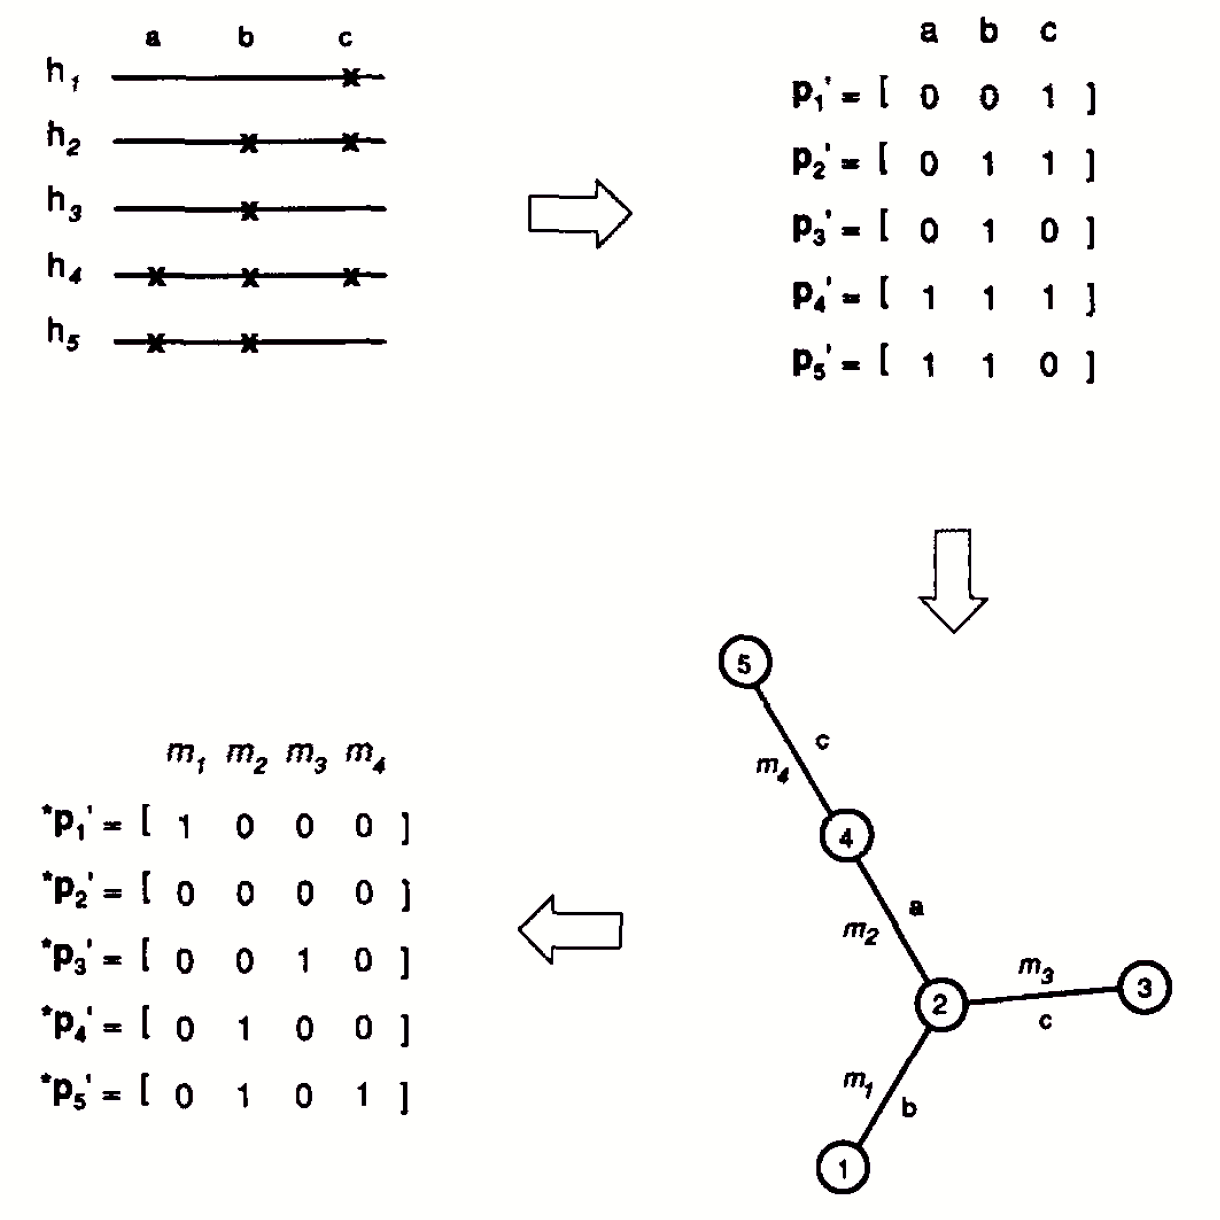
\includegraphics{amova-procedure.eps}}
\end{center}
\caption{Converting raw differences in sequence (or presence and
  absence of restriction sites) into a minimum spanning tree and a
  mutational measure of distance for an analysis of molecular variance~(from~\cite{Excoffier-etal92}).}\label{fig:amova-procedure}
\end{figure}

\section*{An AMOVA example}\index{AMOVA!example}

Excoffier et al.~\cite{Excoffier-etal92} illustrate the approach by
presenting an analysis of restriction haplotypes in human mtDNA. They
analyze a sample of 672 mitochondrial genomes representing two
populations in each of five regional
groups~(Figure~\ref{fig:amova-sample-locations}). They identified 56
haplotypes in that sample. A minimum spanning tree illustrating the
relationships and the relative frequency of each haplotype is
presented in Figure~\ref{fig:amova-haplotypes}.

\begin{figure}
\begin{center}
\resizebox{!}{6cm}{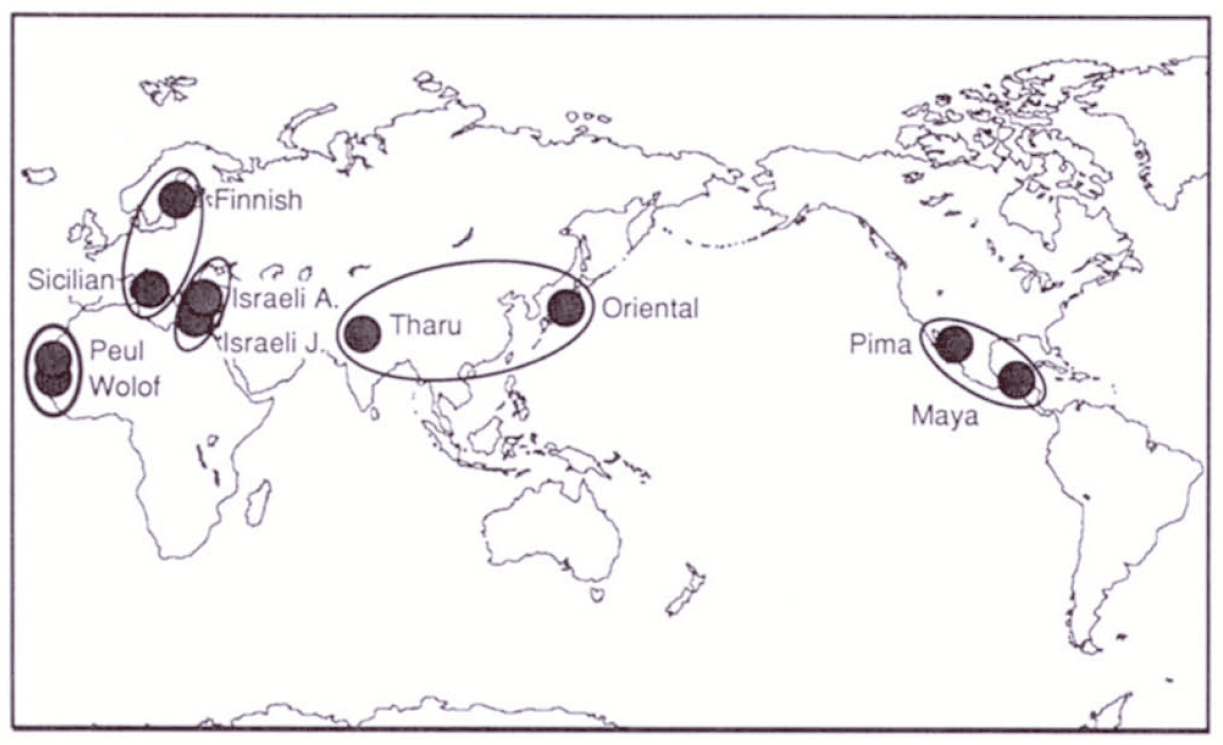
\includegraphics{amova-sample-locations.eps}}
\end{center}
\caption{Locations of human mtDNA samples used in the example
  analysis~(from~\cite{Excoffier-etal92}).}\label{fig:amova-sample-locations}
\end{figure}

\begin{figure}
\begin{center}
\resizebox{!}{6cm}{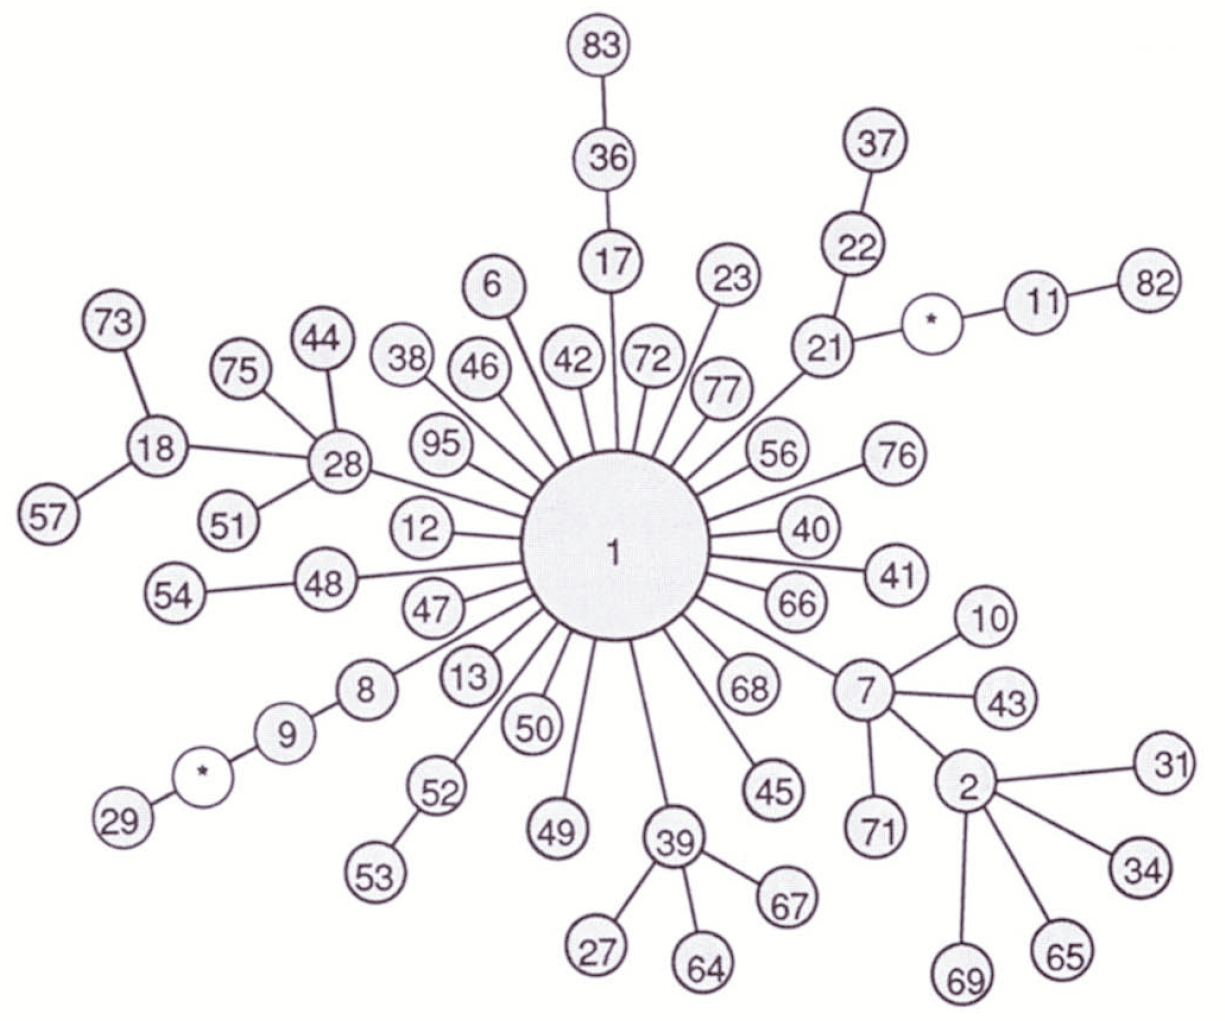
\includegraphics{amova-haplotypes.eps}}
\end{center}
\caption{Minimum spanning network of human mtDNA samples in the
  example. The size of each circle is proportional to its
  frequency~(from~\cite{Excoffier-etal92}).}\label{fig:amova-haplotypes}
\end{figure}

It's apparent from Figure~\ref{fig:amova-haplotypes} that haplotype 1
is very common. In fact, it is present in substantial frequency in
every sampled population. An AMOVA using the minimum spanning network
in Figure~\ref{fig:amova-haplotypes} to measure distance produces the
results shown in Table~\ref{table:amova-results}. Notice that there is
relatively little differentiation among populations within the same
geographical region ($\Phi_{SC} = 0.044$). There is, however,
substantial differentiation among regions ($\Phi_{CT} = 0.220$). In
fact, differences among populations in different regions is
responsible for nearly all of the differences among populations
($\Phi_{ST} = 0.246$).

Remembering that AMOVA partitions a combination of haplotype frequency
differences and haplotye differences, the interpretation of the
$\Phi$-statistics is a little different from the interpretation of
$F$-statistics. When we say that there is relatively little
differentiation among populations within regions and that differences
among populations are responsible for most of the among population
differences, we mean that the evolutionary distance\footnote{Measured
  on the minimum spanning tree.} between any two haplotypes from
populations within the same region is relatively small while the
evolutionary distance between haplotypes from different regions is
relatively large.

Notice also that $\Phi$-statistics follow the same rules as Wright's
$F$-statistics, namely
\begin{eqnarray*}
1 - \Phi_{ST} &=& (1 - \Phi_{SC})(1 - \Phi_{CT}) \\
0.754 &=& (0.956)(0.78) \quad ,
\end{eqnarray*}
within the bounds of rounding error.\footnote{There wouldn't be any
  rounding error if we had access to the raw data.}

\begin{table}
\begin{center}
\begin{tabular}{lc}
\hline\hline
Component of differentiation     & $\Phi$-statistics \\
\hline
Among regions                    & $\Phi_{CT} = 0.220$ \\
Among populations within regions & $\Phi_{SC} = 0.044$ \\
Among all populations            & $\Phi_{ST} = 0.246$ \\
\hline
\end{tabular}
\end{center}
\caption{AMOVA results for the human mtDNA
  sample~(from~\cite{Excoffier-etal92}).}\label{table:amova-results}
\end{table}

\section*{An extension}

As you may recall,\footnote{Look back at our discussion of the
  coalescent
  (\url{http://darwin.eeb.uconn.edu/eeb348-notes/coalescent.pdf}) for
  the details.}  Slatkin~\cite{Slatkin91-coalescence} pointed out that
there is a relationship between coalescence time and $F_{st}$. Namely,
if mutation is rare then
\[
F_{ST} \approx \frac{\bar t - \bar t_0}{\bar t} \quad ,
\]
where $\bar t$ is the average time to coalescence for two genes drawn
at random without respect to population and $\bar t_0$ is the average
time to coalescence for two genes drawn at random from the same
populations. Results in~\cite{Holsinger-MasonGamer96} show that when
$\delta_{ij}$ is linearly proportional to the time since two sequences
have diverged, $\Phi_{ST}$ is a good estimator of $F_{ST}$ when
$F_{ST}$ is thought of as a measure of the relative excess of
coalescence time resulting from dividing a species into several
population. This observation suggests that the combination of
haplotype frequency differences and evolutionary distances among
haplotypes may provide insight into the evolutionary relationships
among populations of the same species.

\bibliography{popgen}
\bibliographystyle{plain}

\ccLicense

\end{document}



\documentclass[12pt]{article}
\usepackage{lecture}
\usepackage{graphicx}
\usepackage{html}
\usepackage{url}
\usepackage{epstopdf}

\newcommand{\copyrightYears}{2010--2021}

\title{Statistical phylogeography: Migrate-N, IMa, and ABC}

\begin{document}

\maketitle

\thispagestyle{first}

Nested clade
analysis~\cite{Templeton-2004,Templeton-2009,Templeton-etal-1995}
represented the earliest attempt to develop a formal approach to using
an estimate of phylogenetic relationships among haplotypes to infer
something both about the biogeographic history of the populations in
which they are contained and the evolutionary processes associated
with the pattern of diversification implied by the phylogenetic
relationships among haplotypes and their geographic distribution. The
statistical parsimony part of NCA depends heavily on coalescent theory
for calculating the ``limits'' of parsimony. As a result, NCA combines
aspects of pure phylogenetic inference{\dash}parsimony{\dash}with
aspects of pure population genetics{\dash}coalescent theory{\dash}to
develop a set of inferences about the phylogeographic history of
populations within species. NCA is now of primarily historical
interest. So far as I am aware, no one uses it any more. Instead
everyone uses methods based directly on coalescent theory or similar
approaches. Before we get to that, though, I need to describe one
complication that is taken for granted now that first became widely
recognized in the late 1980s. Pekka Pamilo and Mashatoshi
Nei~\cite{Pamilo-Nei-1988} pointed out that the phylogenetic
relationships of a single gene might be different from those of the
populations from which the samples were collected.

\section*{Gene trees {\it versus\/} population trees}\index{gene tree}\index{population tree}

There are several reasons why {\it gene trees\/} might not match {\it
  population trees}.

\begin{itemize}

\item It could simply be a problem of estimation. Given a particular
  set of gene sequences, we {\it estimate} a phylogenetic relationship
  among them. But our estimate could be wrong. In fact, given the
  astronomical number of different trees possible with 50 or 60
  distinct sequences, every phylogenetic estimate is virtually certain
  to be wrong somewhere. We just don't know where. So a difference
  between our {\it estimate\/} of a gene tree and the population tree
  could mean nothing more than that they actually match, but our gene
  tree estimate is wrong.

\item There might have been a hybridization event in the past so that
  the phylogenetic history of the gene we're studying is different
  from that of the populations from which we sampled. Hybridization is
  especially likely to have a large impact if the locus for which we
  have information is uniparentally inherited, e.g., mitochondrial or
  chloroplast DNA. A single hybridization event in the distant past in
  which the maternal parent was from a different population will give
  mtDNA or cpDNA a very different phylogeny than nuclear genes that
  underwent a lot of backcrossing after the hybridization event.

\item If the ancestral population was polymorphic at the time the
  initial split occurred alleles that are more distantly related
  might, by chance, end up in the same descendant population~(see
  Figure~\ref{fig:ancestral-polymorphism})\index{ancestral polymorphism}

\end{itemize}

\begin{figure}
\begin{center}
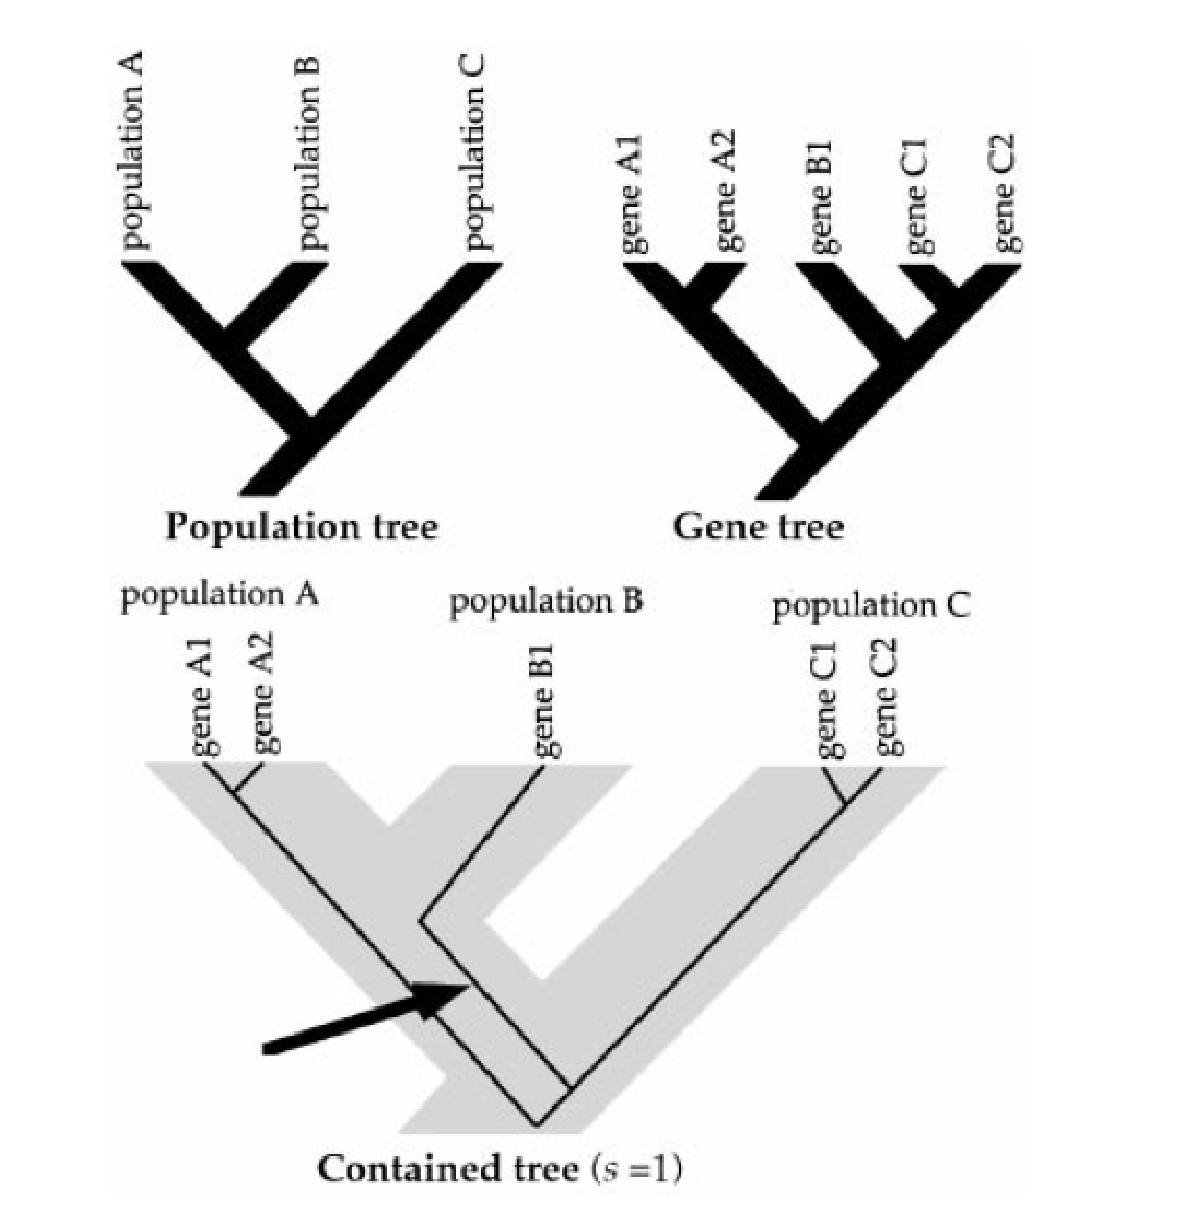
\includegraphics[height=10cm]{ancestral-polymorphism.eps}
\end{center}
\caption{Discordance between gene and population trees as a result of
  ancestral polymorphism
  (from~\cite{Knowles-2001}).}\label{fig:ancestral-polymorphism} 
\end{figure}

As Pamilo and Nei showed, it's possible to calculate the probability
of discordance between the gene tree and the population tree using
some basic ideas from coalescent theory. That leads to a further
refinement, using coalescent theory directly to examine alternative
biogeographic hypotheses.

\section*{Coalescent-based estimates of migration rate}

Peter Beerli and Joe
Felsenstein~\cite{Beerli-Felsenstein-1999,Beerli-Felsenstein-2001}
proposed a coalescent-based method to estimate migration rates among
populations. As with other analytical methods we've encountered in
this course, the details can get pretty hairy, but the basic idea is
(relatively) simple.\index{coalescent!migration}

Recall that in a single population we can describe the coalescent
history of a sample without too much difficulty. Specifically, given a
sample of $k$ alleles in a diploid population with effective size
$N_e$, the probability that the first coalescent event took place $t$
generations ago is
\begin{equation}
P(t|k, N_e) = \left(\frac{k(k-1)}{4N_e}\right)\left(1-
  \frac{k(k-1)}{4N_e}\right)^{t-1} \quad . \label{eq:coalescent-single}
\end{equation}
Now suppose that we have a sample of alleles from $K$ different
populations. To keep things (relatively) simple, we'll imagine that we
have a sample of $n$ alleles from every one of these populations and
that every population has an effective size of $N_e$. In addition,
we'll imagine that there is migration among populations, but again
we'll keep it really simple. Specifically, we'll assume that the
probability that a given allele in our sample from one population had
its ancestor in a different population in the immediately preceding
generation is $m$.\footnote{In other words, $m$ is the backwards
  migration rate, the probability that a gene in one population came
  from another population in the preceding generation. This is the
  same migration rate we encountered weeks ago when we discussed the
  balance between drift and migration. The method Beerli and
  Felsenstein developed allows populations to differ in $N_e$ and
  allows rates of migration among pairs of populations to differ. It
  even allows the rate of migration into population A from population
  B to differ from the rate of migration into population B from
  population A. We're going to ignore all of those complications here,
  because the math is complicated enough without them, and it gets a
  {\it lot\/} more complicated when they are included.} Under this
simple scenario, we can again construct the coalescent history of our
sample. How? Funny you should ask.

We start by using the same logic we used to construct
equation~(\ref{eq:coalescent-single}). Specifically, we ask ``What's
the probability of an `event' in the immediately preceding
generation?'' The complication is that there are two kinds of events
possible: 

\begin{enumerate}

\item a coalescent event and 

\item a migration event. 

\end{enumerate}

\noindent As in our original development of the coalescent process,
we'll assume that the population sizes are large enough that the
probability of two coalescent events in a single time step is so small
as to be negligible. In addition, we'll assume that the number of
populations and the migration rates are small enough that the
probability of more than one event of either type is so small as to be
negligible. That means that all we have to do is to calculate the
probability of either a coalescent event or a migration event and
combine them to calculate the probability of an event. It turns out
that it's easiest to calculate the probability that there {\it
  isn't\/} an event first and then to calculate the probability that
there is an event as one minus that.

We already know that the probability of a coalescent event in
population $k$, is
\[
P_k(\mbox{coalescent}|n, N_e) = \frac{k(k-1)}{4N_e} \quad ,
\]
so the probability that there is {\it not\/} a coalescent event in any
of our $K$ populations is
\[
P(\mbox{no coalescent}|k, N_e, K) = \left(1-\frac{k(k-1)}{4N_e}\right)^K
\quad .
\]
If $m$ is the probability that there was a migration event in a
particular population than the probability that there is {\it not\/} a
migration event involving any of our $kK$ alleles\footnote{$K$ populations
each with $k$ alleles} is
\[
P(\mbox{no migration}|k,m, K) = (1-m)^{kK} \quad .
\]
So the probability that there {\it is\/} an event of some kind is
\[
P(\mbox{event}|k, m, N_e, K) = 1 - P(\mbox{no coalescent}|k, N_e,
K)P(\mbox{no migration}|k,m, K) \quad .\label{eq:event}
\]
Now we can calculate the time back to the first event
\[
P(\mbox{event at }t|k, m, N_e, K) = P(\mbox{event}|k, m, N_e,
K)\left(1 - P(\mbox{event}|k, m, N_e, K)\right)^{t-1} \quad . \label{eq:time-to-event}
\]
We can then use Bayes theorem to calculate the probability that the
event was a coalescence or a migration and the population or
populations involved. Notice, however, that if the event is a
coalescent event, we first have to pick the population in which it
occurred and then identify the pair of alleles that coalesced. Alleles
have to be in the same population. Once we've done all of this, we
have a new population configuration and we can start over. We continue
until all of the alleles have coalesced into a single common ancestor,
and then we have the complete coalescent history of our
sample.\footnote{This may not seem very simple, but just think about
  how complicated it would be if I allowed every population to have a
  different effective size and if I allowed each pair of populations
  to have different migration rates between them.} That's roughly the
logic that Beerli and Felsenstein use to construct coalescent
histories for a sample of alleles from a set of
populations{\dash}except that they allow effective population sizes to
differ among populations and they allow migration rates to differ
among all pairs of populations. As if that weren't bad enough, now
things start to get even more complicated.

There are lots of different coalescent histories possible for a sample
consisting of $n$ alleles from each of $K$ different populations, even
when we fix $m$ and $N_e$. Worse yet, given any one coalescent
history, there are a lot of different possible mutational histories
possible. In short, there are a lot of different possible sample
configurations consistent with a given set of migration rates and
effective population size. Nonetheless, some combinations of $m$ and
$N_e$ will make the data more likely than others. In other words, we
can construct a likelihood for our data:
\[
P(\mbox{data}|m, N_e) \propto f(n, m, N_e, K) \quad ,
\]
where $f(n, m, N_e,K)$ is some very complicated function of the
probabilities we derived above. In fact, the function is so
complicated, we can't even write it down. Fortunately, Beerli and
Felsenstein, being very clever people, figured out a way to simulate
the likelihood, and {\tt Migrate-n}
\url{http://popgen.sc.fsu.edu/Migrate/Migrate-n.html} provides a
(relatively) simple way that you can use your data to estimate $m$ and
$N_e$ for a set of populations. In fact, {\tt Migrate-N} will allow
you to estimate pairwise migration rates among all populations in your
sample, and since it can simulate a likelihood, if you put priors on
the parameters you're interested in, i.e., $m$ and $N_e$, you can get
Bayesian estimates of those parameters rather than maximum likelihood
estimates, including credible intervals around those estimates so that
you have a good sense of how reliable your estimates are.\footnote{If
  you'd like to see a comparision of maximum likelihood and Bayesian
  approaches, Beerli~\cite{Beerli-2006} provides an excellent
  overview.}\index{coalescent!estimating migration
  rates}\index{migration!estimating}\index{Migrate-N@{\tt Migrate-N}}

There's one further complication I need to mention, and it involves a
lie I just told you. {\tt Migrate-N} can't give you estimates of $m$
and $N_e$. Remember how every time we've dealt with drift and another
process we always end up with things like $4N_em$, $4N_e\mu$, and the
like. Well, the situation is no different here. What {\tt Migrate-N} can
actually estimate are the two parameters $4N_em$ and
$\theta=4N_e\mu$.\footnote{Depending on the option you pick when you
  run {\tt Migrate} you can either get $\theta$ and $4N_em$ or
  $\theta$ and $M=m/\mu$.} How did $\mu$ get in here when I only
mentioned it in passing? Well, remember that I said that once the
computer has constructed a coalescent history, it has to apply
mutations to that history. Without mutation, all of the alleles in our
sample would be identical to one another. Mutation is what 
produces the diversity. So what we get from {\tt Migrate-N} isn't the
fraction of a population that's composed of migrants. Rather, we get
an estimate of how much migration contributes to local population
diversity relative to mutation. That's a pretty interesting estimate
to have, but it may not be everything that we want.

There's a further complication to be aware of. Think about the
simulation process I described. All of the alleles in our sample are
descended from a single common ancestor. That means we are implicitly
assuming that the set of populations we're studying have been around
long enough and have been exchanging migrants with one another long
enough that we've reached a drift-mutation-migration equilibrium. If
we're dealing with a relatively small number of populations in a
geographically limited area, that may not be an unreasonable
assumption, but what if we're dealing with populations of crickets
spread across all of the northern Rocky Mountains? And what if we
haven't sampled all of the populations that
exist?\footnote{Beerli~\cite{Beerli-2004} discusses the impact of
  ``ghost'' populations. He concludes that you have to be careful
  about which populations you sample, but that you don't necessarily
  need to sample every population. Read the paper for the details.} In
many circumstances, it may be more appropriate to imagine that
populations diverged from one another at some time in the not too
distant past, have exchanged genes since their divergence, but haven't
had time to reach a drift-mutation-migration equilibrium. What do we
do then?

\section*{Divergence and migration}

Rasmus Nielsen and John Wakely~\cite{Nielsen-Wakeley-2001} consider
the simplest generalization of Beerli and
Felsenstein~\cite{Beerli-Felsenstein-1999,Beerli-Felsenstein-2001} you
could imagine~(Figure~\ref{fig:nielsen-wakeley}). They consider a
situation in which you have samples from only two populations and
you're interested in determining both how long ago the populations
diverged from one another and how much gene exchange there has been
between the populations since they diverged. As in {\tt Migrate-N}
mutation and migration rates are confounded with effective population
size, and the relevant parameters become:\index{coalescent!estimating
  migration}\index{coalescent!diverging populations}

\begin{itemize}

\item $\theta_a$, which is $4N_e\mu$ in the ancestral population.

\item $\theta_1$, which is $4N_e\mu$ in the first population.

\item $\theta_2$, which is $4N_e\mu$ in the second population.

\item $M_1$, which is $2N_em_1$ in the first population, where $m_1$ is
  the fraction of the first population composed of migrants from the
  second population.

\item $M_2$, which is $2N_em_2$ in the second population.

\item $T$, which is the time since the populations
  diverged. Specifically, if there have been $t$ units since
  the two populations diverged, $T=t/2N_1$, where $N_1$ is the
  effective size of the first population.

\end{itemize}

\begin{figure}
\begin{center}
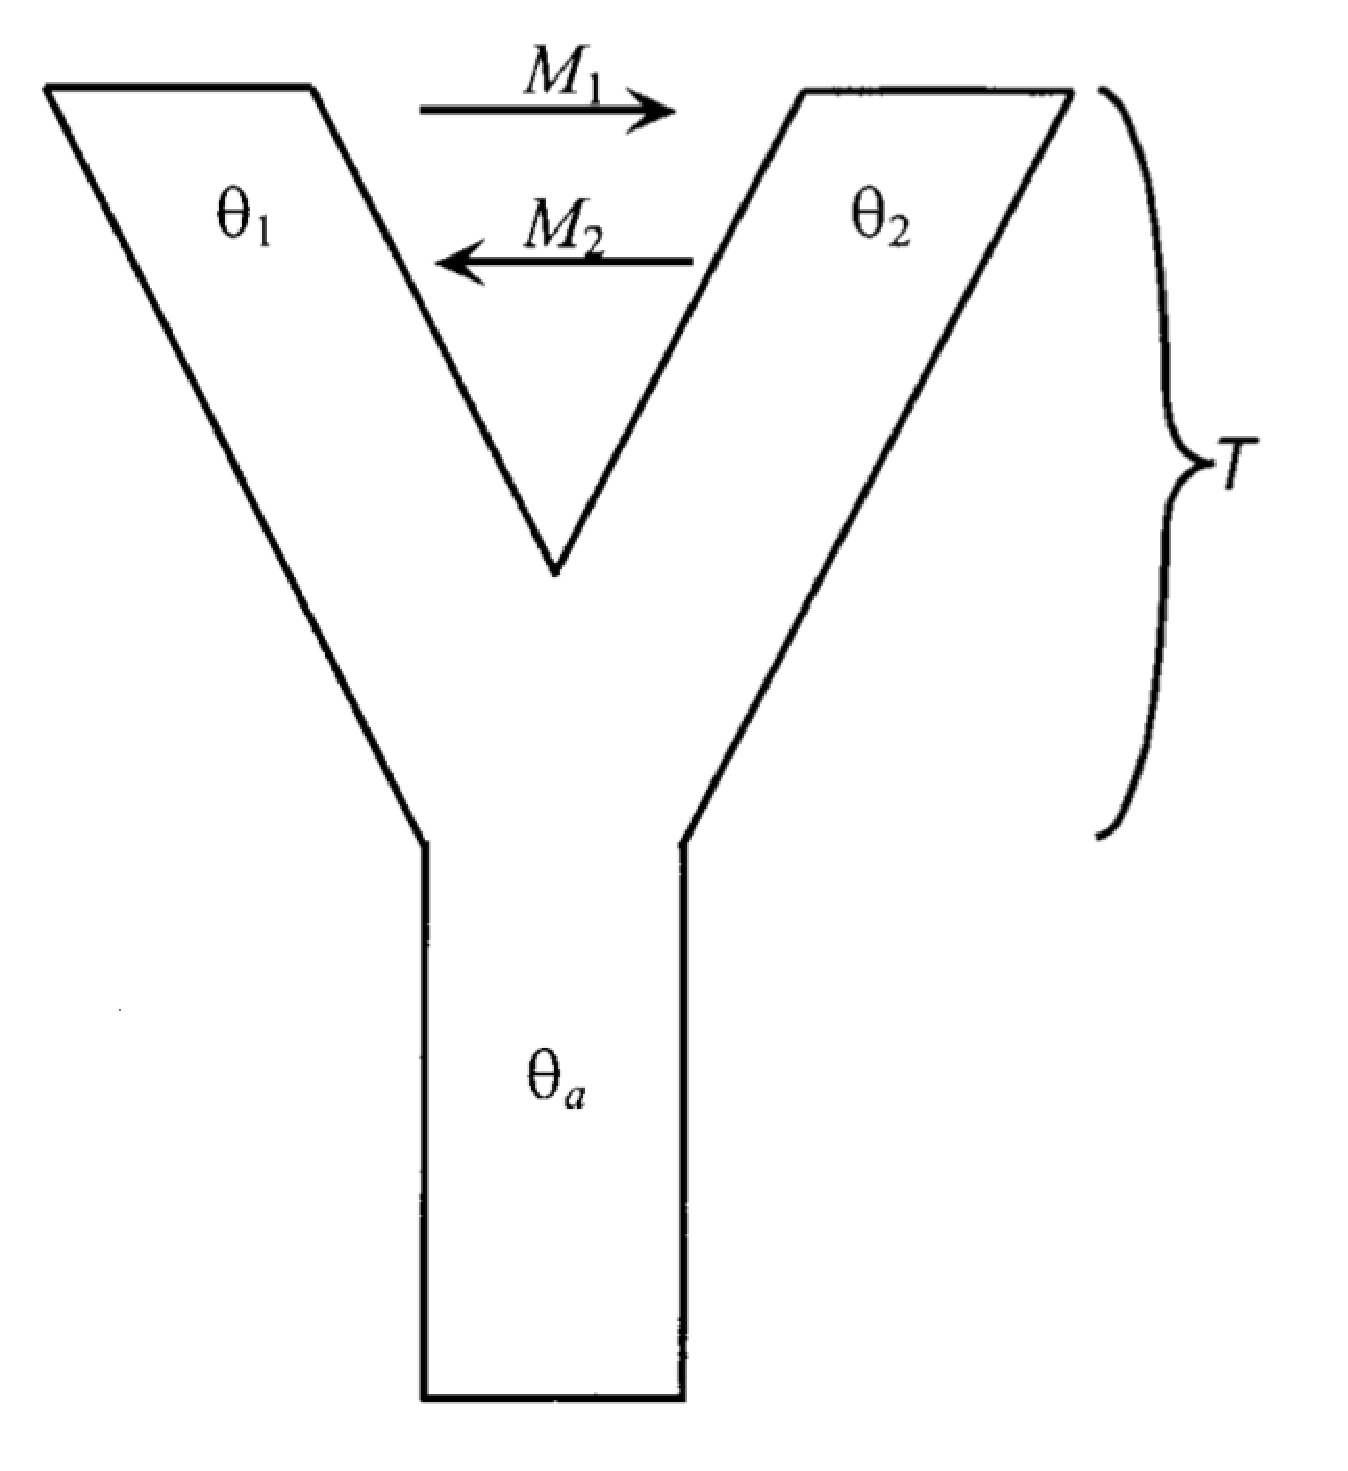
\includegraphics[height=6cm]{nielsen-wakeley.eps}
\end{center}
\caption{The simple model developed by Nielsen and
  Wakeley~\cite{Nielsen-Wakeley-2001}. $\theta_a$ is $4N_e\mu$ in the
  ancestral population; $\theta_1$ and $\theta_2$ are $4N_e\mu$ in the
  descendant populations; $M_1$ and $M_2$ are $2N_em$, where $m$ is
  the backward migration rate; and $T$ is the time since divergence of
  the two populations.}\label{fig:nielsen-wakeley}
\end{figure}

Given that set of parameters, you can probably imagine that you can
calculate the likelihood of the data for a given set of
parameters.\footnote{As with {\tt Migrate-N}, you can't calculate the
  likelihood explicitly, but you can approximate it
  numerically. See~\cite{Nielsen-Wakeley-2001} for details.} Once you
can do that you can either obtain maximum-likelihood estimates of the
parameters by maximizing the likelihood, or you can place prior
distributions on the parameters and obtain Bayesian estimates from the
posterior distribution. Either way, armed with estimates of
$\theta_a$, $\theta_1$, $\theta_2$, $M_1$, $M_2$, and $T$ you can say
something about:

\begin{enumerate}

\item the effective population sizes of the two populations relative
  to one another and relative to the ancestral population, 

\item the relative frequency with which migrants enter each of the two
  populations from the other, and 

\item the time at which the two populations diverged from one another.

\end{enumerate}

\noindent Keep in mind, though, that the estimates of $M_1$ and $M_2$
confound local effective population sizes with migration rates. So if
$M_1 > M_2$, for example, it does not mean that the fraction of
migrants incorporated into population 1 exceeds the fraction
incorporated into population 2. It means that the {\it number\/} of
migrants entering population 1 is greater than the number entering
population 2.

\subsection*{An example}

Orti et al.~\cite{Orti-etal-1994} report the results of phylogenetic
analyses of mtDNA sequences from 25 populations of threespine
stickleback, {\it Gasterosteus aculeatus}, in Europe, North America,
and Japan. The data consist of sequences from a 747bp fragment of
cytochrome $b$. Nielsen and Wakely~\cite{Nielsen-Wakeley-2001} analyze
these data using their approach. Their analyses show that ``[a] model
of moderate migration and very long divergence times is more
compatible with the data than a model of short divergence times and
low migration rates.'' By ``very long divergence times'' they mean $T
> 4.5$, i.e., $t > 4.5N_1$. Focusing on populations in the western
(population 1) and eastern Pacific (population 2), they find that the
maximum likelihood estimate of $M_1$ is 0, indicating that there is
little if any gene flow from the eastern Pacific (population 2) into
the western Pacific (population 1). In contrast, the maximum
likelihood estimate of $M_2$ is about 0.5, indicating that one
individual is incorporated into the eastern Pacific population from
the western Pacific population every other generation. The
maximum-likelihood estimates of $\theta_1$ and $\theta_2$ indicate
that the effective size of the population eastern Pacific population
is about 3.0 times greater than that of the western Pacific
population.

\subsection*{Extending the approach to multiple populations}

Jody Hey later announced the release of {\tt IMa2}.\footnote{Available
  from \url{https://bio.cst.temple.edu/~hey/software/software.htm}.}
Building on work described in Hey and
Nielsen~\cite{Hey-Nielsen-2004,Hey-Nielsen-2007}, {\tt IMa2} allows
you to estimate relative divergence times, relative effective
population sizes, and relative pairwise migration rates for more than
two populations at a time. That flexibility comes at a cost, of
course. In particular, you have to specify the phylogenetic history of
the populations before you begin the analysis.

\section*{Phylogeography of montane grasshoppers}

Lacey Knowles studied grasshoppers in the genus {\it Melanopus}. She
collected 1275bp of DNA sequence data from cytochrome oxidase I (COI)
from 124 individuals of {\it M. oregonensis\/} and two outgroup
species. The specimens were collected from 15 ``sky-island'' sites in
the northern Rocky Mountains~(see Figure~\ref{fig:sky-islands};
\cite{Knowles-2001}). Two alternative hypotheses had been proposed to
describe the evolutionary relationships among these
grasshoppers~(refer to Figure~\ref{fig:divergence-hypotheses} for a
pictorial representation):\index{Melanopus@\textit{Melanopus}}

\begin{figure}
\begin{center}
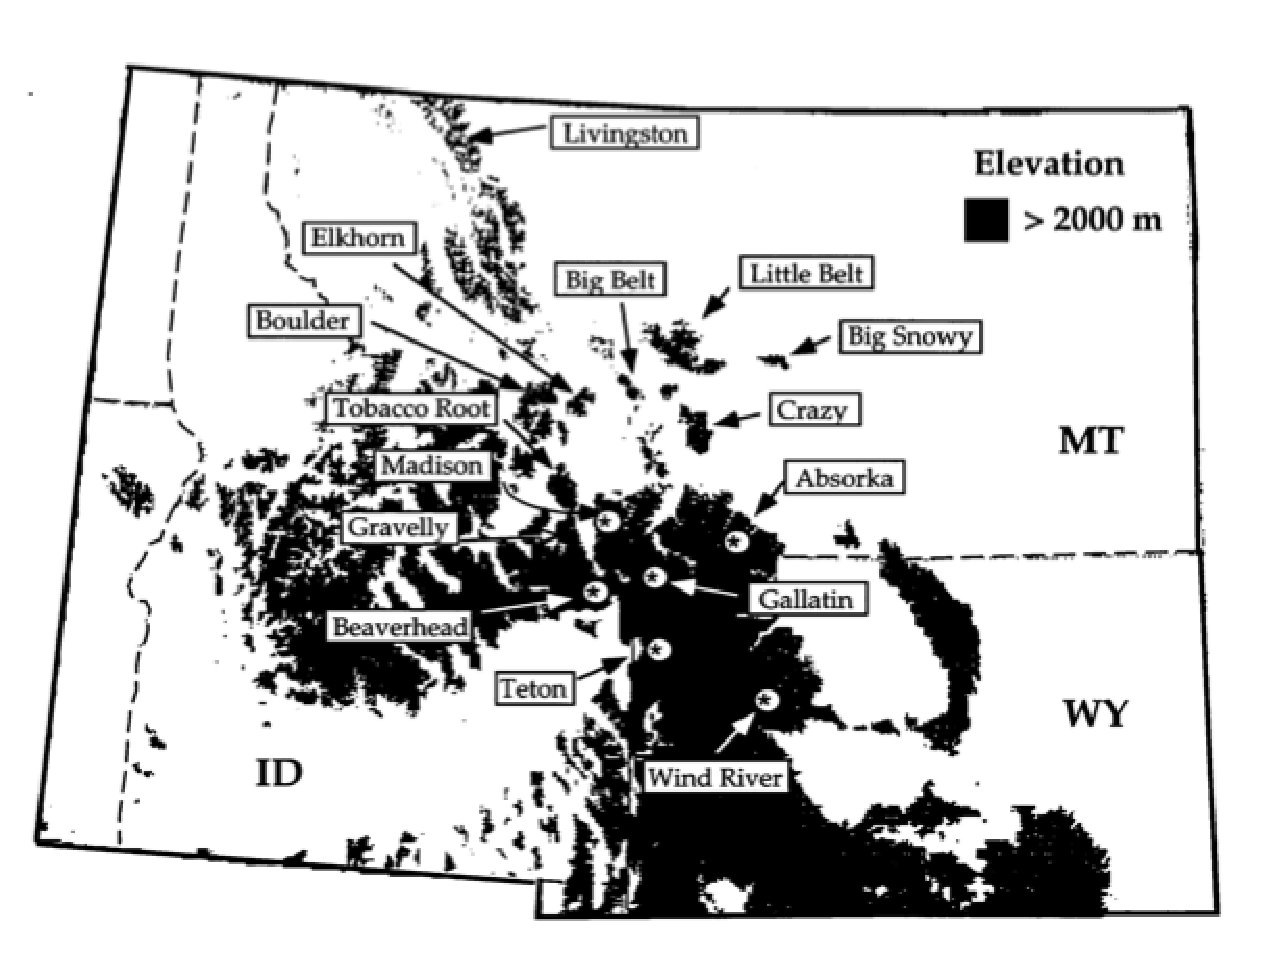
\includegraphics[height=6cm]{sky-islands.eps}
\end{center}
\caption{Collection sites for {\it Melanopus oregonensis\/} in the
  northern Rocky Mountains~(from~\cite{Knowles-2001}).}\label{fig:sky-islands}
\end{figure}

\begin{itemize}

\item {\bf Widespread ancestor}: The existing populations might represent
  independently derived remnants of a single, widespread
  population. In this case all of the populations would be equally
  related to one another.

\item {\bf Multiple glacial refugia}: Populations that shared the same
  refugium will be closely related while those that were in different
  refugia will be distantly related.

\end{itemize}

\begin{figure}
\begin{center}
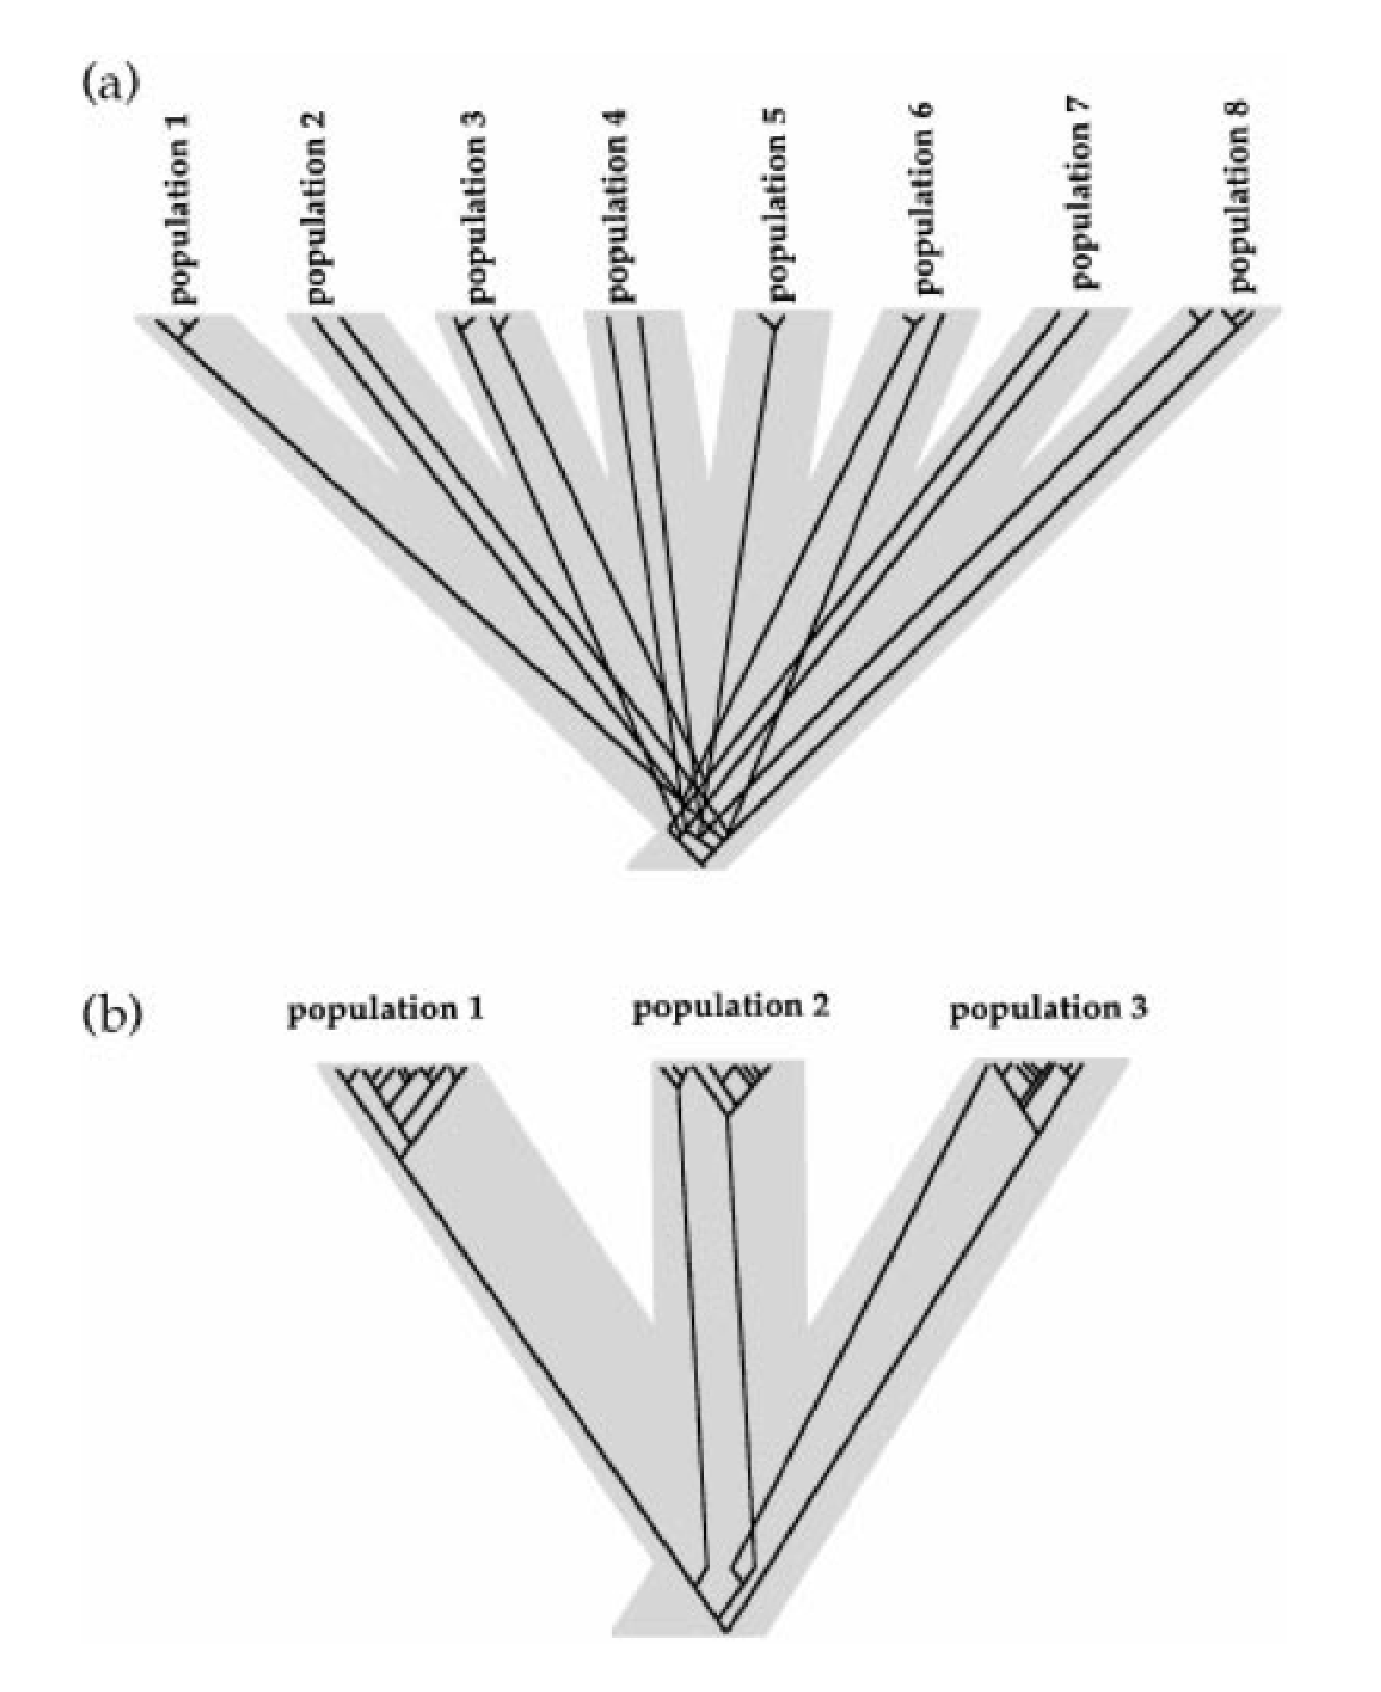
\includegraphics[height=6cm]{divergence-hypotheses.eps}
\end{center}
\caption{Pictorial representations of the ``widespread ancestor''
  (top) and ``glacial refugia'' (bottom)
  hypotheses~(from~\cite{Knowles-2001}).}\label{fig:divergence-hypotheses}
\end{figure}

As is evident from Figure~\ref{fig:divergence-hypotheses}, the two
hypotheses have very different consequences for the coalescent history
of alleles in the sample. Since the interrelationships between
divergence times and time to common ancestry differ so markedly
between the two scenarios, the pattern of sequence differences found
in relation to the geographic distribution will differ greatly between
the two scenarios. 

Using techniques described in Knowles and
Maddison~\cite{Knowles-Maddison-2002}, Knowles simulated gene trees
under the widespread ancestor hypothesis. She then placed them within
a population tree representing the multiple glacial refugia hypothesis
and calculated a statistic, $s$, that measures the discordance between
a gene tree and the population tree that contains it. This gave her a
distribution of $s$ under the widespread ancestor hypothesis. She
compared the $s$ estimated from her actual data with this distribution
and found that the observed value of $s$ was only 1/2 to 1/3 the size
of the value observed in her simulations.\footnote{The discrepancy was
  largest when divergence from the widespread ancestor was assumed to
  be very recent.} Let's unpack that a bit. 

\begin{itemize}

\item Knowles estimated the phylogeny of the haplotypes in her
  sample. $s$ is the estimated minimum number of among-population
  migration events necessary to account for where haplotypes are
  currently found given the inferred
  phylogeny~\cite{Slatkin-Maddison-1989}. Let's call the $s$ estimated
  from the data $s_{obs}$.

\item Then she simulated a neutral coalescence process in which the
  populations were derived from a single, widespread ancestral
  population. For each simulation she rearranged the data so that
  populations were grouped into separate refugia and estimated $s_{sim}$
  from the rearranged data, and she repeated this 100 times for
  several different times since population splitting.

\end{itemize}

\noindent The results are shown in
Figure~\ref{fig:knowles-s-values}. As you can see, the observed $s$
value is much smaller than any of those obtained from the coalescent
simulations. That means that the observed data require far fewer
among-population migration events to account for the observed
geographic distribution of haplotypes than would be expected with
independent origin of the populations from a single, widespread
ancestor. In short, Knowles presented strong evidence that her data
are not consistent with the widespread ancestor
hypothesis.\index{statistical phylogeography!example}

\begin{figure}
\begin{center}
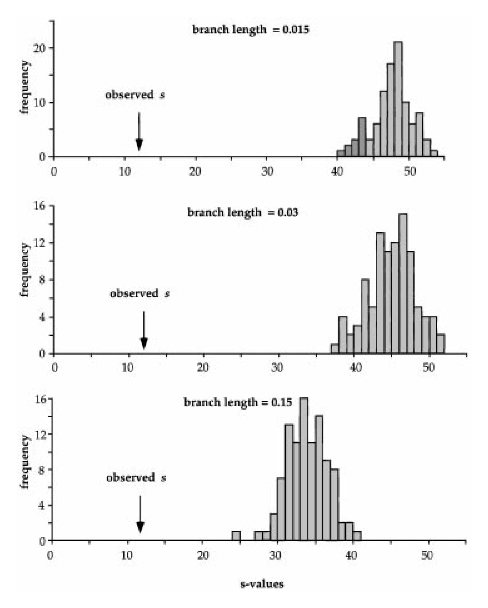
\includegraphics[height=10cm]{knowles-s-values.eps}
\end{center}
\caption{Distribution of the observed minimum number of
  among-population migration events, $s$, and the expected minimum
  number of migration events under the ``widespread ancestor''
  hypothesis.~(from~\cite{Knowles-2001}).}\label{fig:knowles-s-values}
\end{figure}

\section*{Approximate Bayesian computation: motivation}\index{ABC}\index{Approximate Bayesian Computation}

Approximate Bayesian Computation (ABC for short), extends the basic
idea Knowles used to consider more complicated scenarios. The {\tt
  IMa} approach developed by Nielsen, Wakely, and Hey is potentially
{\it very\/} flexible and {\it very\/}
powerful~\cite{Hey-Nielsen-2004,Hey-Nielsen-2007,Nielsen-Wakeley-2001}. It
allows for non-equilibrium scenarios in which the populations from
which we sampled diverged from one another at different times, but
suppose that we think our populations have dramatically increased in
size over time (as in humans) or dramatically changed their
distribution (as with an invasive species). Is there a way to use
genetic data to gain some insight into those processes? Would I be
asking that question if the answer were ``No''?

\section*{An example}

Let's change things up a bit this time and start with an example of a
problem we'd like to solve first. Once you see what the problem is,
then we can talk about how we might go about solving it. The case
we'll discuss is the case of the cane toad, {\it Bufo marinus}, in
Australia.\index{Bufo@\textit{Bufo}!\textit{marinus}}

You may know that the cane toad is native to the American tropics. It
was purposely introduced into Australia in 1935 as a biocontrol agent,
where it has spread across an area of more than 1 million km$^2$. Its
range is still expanding in northern Australia and to a lesser extent
in eastern
Australia~(Figure~\ref{fig:cane-toad-expansion}).\footnote{All of this
  information is from the introduction to~\cite{Estoup-etal-2004}.}
Estoup et al.~\cite{Estoup-etal-2004} collected microsatellite data
from 30 individuals in each of 19 populations along roughly linear
transects in the northern and eastern expansion areas.

\begin{figure}
\begin{center}
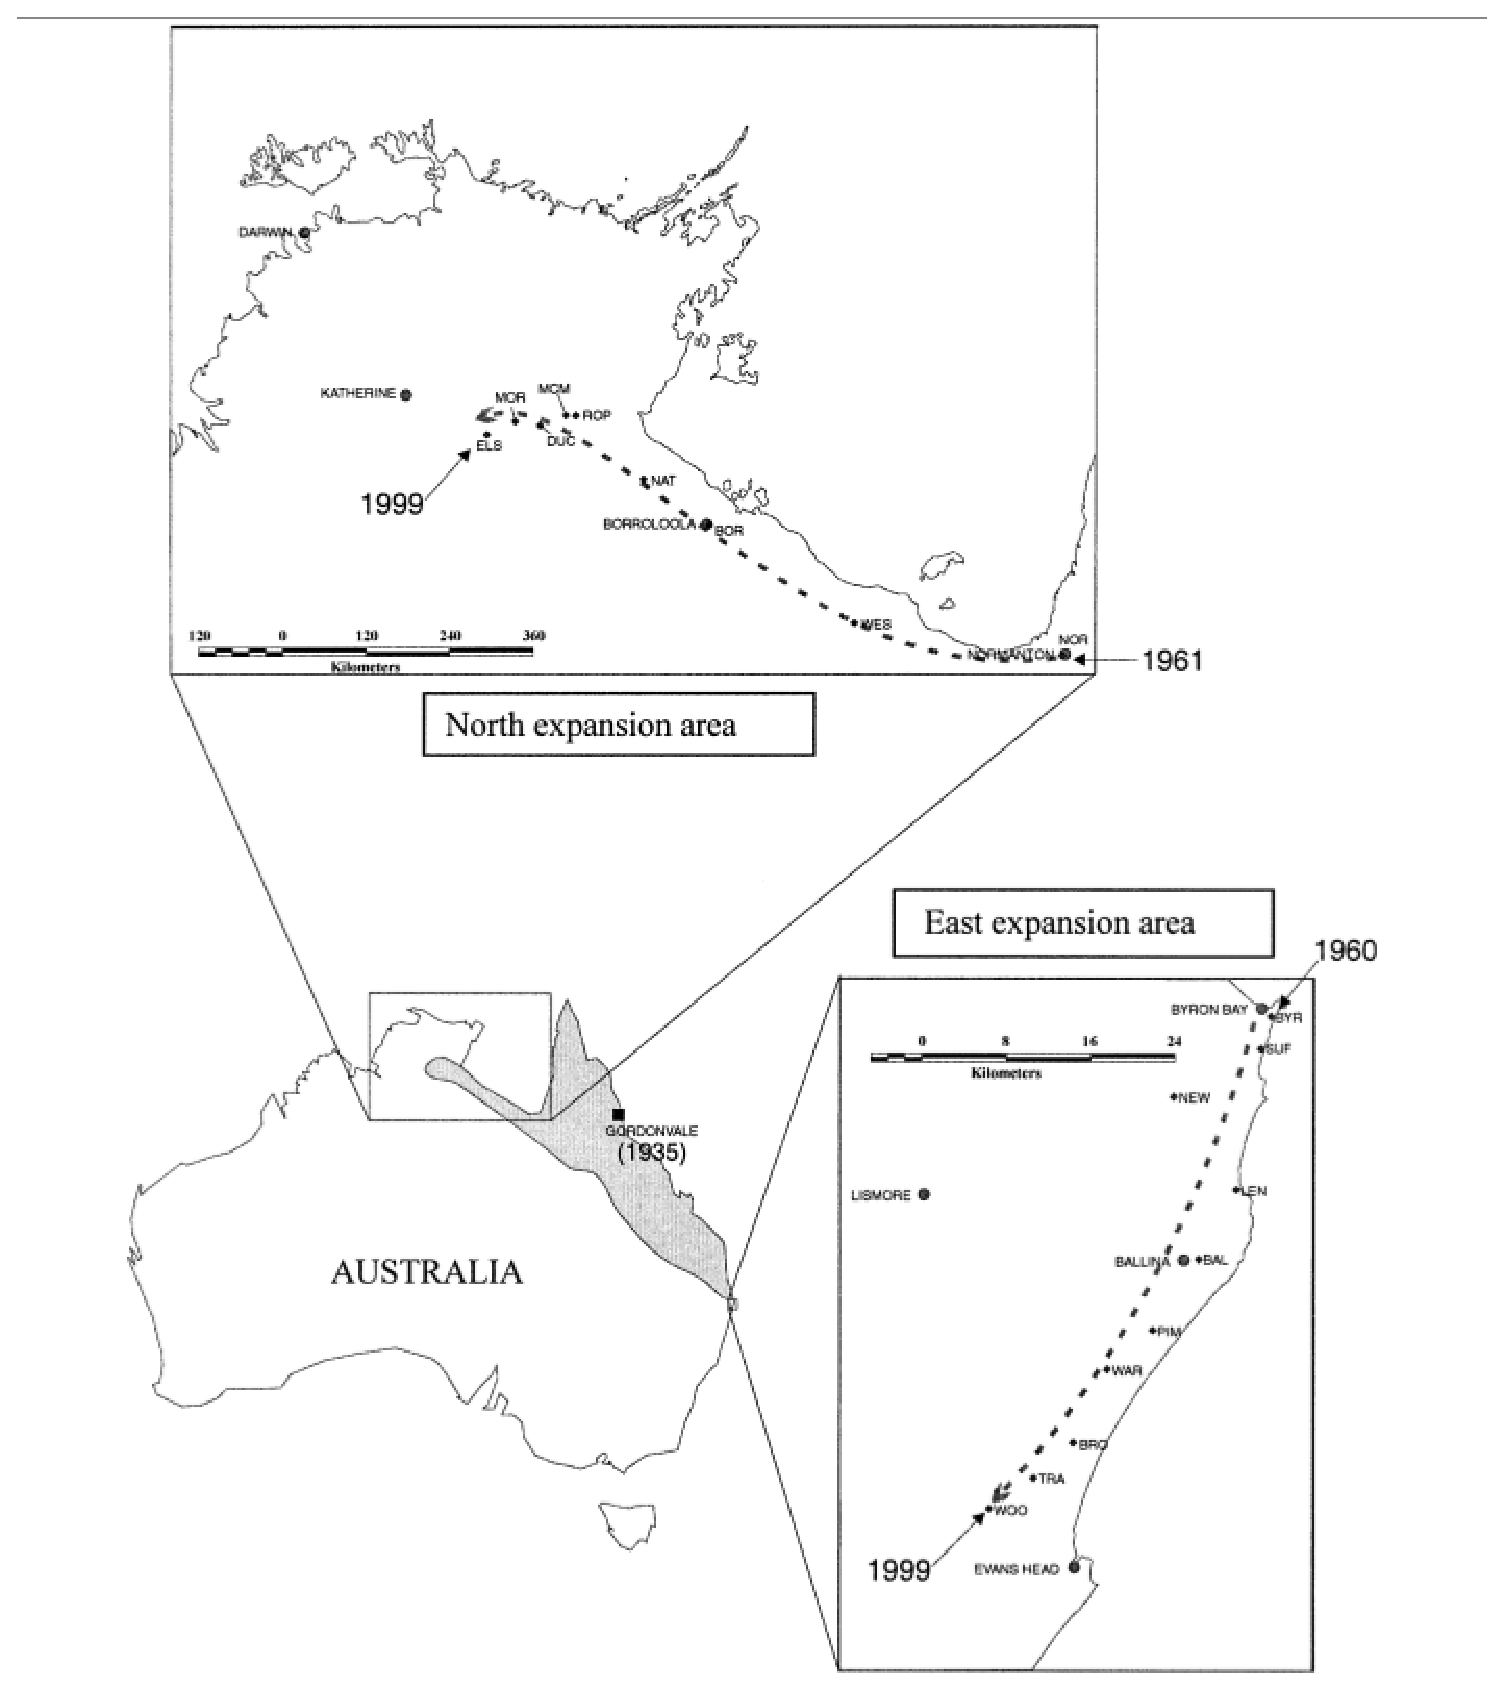
\includegraphics[width=6.0in]{cane-toad-expansion.eps}
\end{center}
\caption{Maps showing the expansion of the cane toad population in
  Australia since its introduction in 1935~(from~\cite{Estoup-etal-2004}).}\label{fig:cane-toad-expansion}
\end{figure}

With these data they wanted to distinguish among five possible
scenarios describing the geographic spread:

\begin{itemize}

\item {\bf Isolation by distance}: As the expansion proceeds, each new
  population is founded by or immigrated into by individuals with a
  probability proportional to the distance from existing populations.

\item {\bf Differential migration and founding}: Identical to the
  preceding model except that the probability of founding a population
  may be different from the probability of immigration into an
  existing population.

\item {\bf ``Island'' migration and founding}: New populations are
  established from existing populations without respect to the
  geographic distances involved, and migration occurs among
  populations without respect to the distances involved.

\item {\bf Stepwise migration and founding with founder events}: Both
  migration and founding of populations occurs only among immediately
  adjacent populations. Moreover, when a new population is
  established, the number of individuals involved may be very small.

\item {\bf Stepwise migration and founding without founder events}:
  Identical to the preceding model except that when a population is
  founded its size is assumed to be equal to the effective population
  size. 

\end{itemize}

That's a pretty complex set of scenarios. Clearly, you could use {\tt
  Migrate} or {\tt IMa2} to estimate parameters from the data Estoup
et al.~\cite{Estoup-etal-2004} report, but would those parameters
allow you to distinguish those scenarios? Not in any straightforward
way that I can see. Neither {\tt Migrate} nor {\tt IMa2} distinguishes
between founding and migration events for example. And with {\tt IMa2}
we'd have to specify the relationships among our sampled populations
before we could make any of the calculations. In this case we want to
test alternative hypotheses of population relationship. So what do we
do?

\section*{Approximate Bayesian Computation}\index{Approximate Bayesian Computation}

Well, in principle we could take an approach similar to what {\tt
  Migrate} and {\tt IMa2} use. Let's start by reviewing what we did
last time\footnote{More accurately, what Peter Beerli, Joe
  Felsenstein, Rasmus Nielsen, John Wakeley, and Jody Hey did.} with
{\tt Migrate} and {\tt IMa2}. In both cases, we knew how to simulate
data given a set of mutation rates, migration rates, local effective
population sizes, and times since divergence. Let's call that whole,
long string of parameters $\xi$ and our big, complicated data set
$X$. If we run enough simulations, we can keep track of how many of
those simulations produce data identical to the data we
collected. With those results in hand, we can estimate $P(X|\xi)$,
the likelihood of the data, as the fraction of simulations that
produce data identical to the data we collected.\footnote{The actual
  implementation is a bit more involved than this, but that's the
  basic idea.} In principle, we could take the same approach in this,
much more complicated, situation. But the problem is that there are an
astronomically large number of different possible coalescent histories
and different allelic configurations possible with any one population
history both because the population histories being considered are
pretty complicated and because the coalescent history of every locus
will be somewhat different from the coalescent history at other
loci. As a result, the chances of getting {\it any\/} simulated
samples that match our actual samples is virtually nil, and we can't
estimate $P(X|\xi)$ in the way we have so far.

Approximate Bayesian computation is an approach that allows us to get
around this problem. It was introduced by Beaumont et
al.~\cite{Beaumont-etal-2002} precisely to allow investigators to get
approximate estimates of parameters and data likelihoods in a Bayesian
framework. Again, the details of the implementation get pretty
hairy,\footnote{You're welcome to read the Methods
  in~\cite{Beaumont-etal-2002}, and feel free to ask questions if
  you're interested. I have to confess that there's a decent chance I
  won't be able to answer your question until I've done some further
  studying. I've only used ABC a little, and I haven't used it for
  anything that I've published{\dash}yet.} but the basic idea is relatively
straightforward.\footnote{OK. This maybe calling it ``relatively
  straightforward'' is misleading. Even this simplified outline is
  fairly complicated, but compared to some of what you've already
  survived in this course, it may not look too awful.}

\begin{enumerate}

\item Calculate ``appropriate'' summary statistics for your data set,
  e.g., pairwise estimates of $\phi_{ST}$ (possibly one for every
  locus if you're using microsatellite or SNP data), estimates of
  within population diversity, counts of the number of segregating
  sites~(for nucleotide sequence data, both within each population and
  across the entire sample) or counts of the number of segregating
  alleles~(for microsatellite data). Call that set of summary
  statistics $S$.

\item Specify a prior distribution for the unknown parameters, $\xi$.

\item Pick a random set of parameter values, $\xi'$ from the prior
  distribution and simulate a data set for that set of parameter
  values.

\item Calculate the same summary statistics for the simulated
  data set as you calculated for your actual data. Call that set of
  statistics $S'$. 

\item Calculate the distance between $S$ and $S'$.\footnote{You could
    use any one of a variety of different distance measures. A simple
    Euclidean distance might be useful, but you could also try
    something more complicated, like a Mahalanobis distance.} Call it
  $\delta$. If it's less than some value you've decided on,
  $\delta^*$, keep track of $S'$ and the associated $\xi'$ and
  $\delta$. Otherwise, throw all of them away and forget you ever saw
  them.

\item Return to step 2 and repeat until you have accepted a large
  number of pairs of $S'$ and $\xi'$.

\end{enumerate}

Now you have a bunch of $S'$s and a bunch of $\xi'$s that produced
them. Let's label them $S_i$ and $\xi_i$, and let's remember what
we're trying to do. We're trying to estimate $\xi$ for our real
data. What we have from our real data is $S$. So far it seems as if
we've worked our computer pretty hard, but we haven't made any
progress. 

Here's where the trick comes in. Suppose we fit a regression to the
data we've simulated
\[
\xi_i = \alpha + S_i\beta + \epsilon \quad ,
\]
where $\alpha$ is an intercept, $\beta$ is a vector of regression
coefficients relating each of the summary statistics to $\xi$, and
$\epsilon$ is an error vector.\footnote{I know what you're thinking to
  yourself now. This doesn't sound very simple. Trust me. It is as
  simple as I can make it. The actual procedure involves local linear
  regression. I'm also not telling you how to go about picking
  $\delta$ or how to pick ``appropriate'' summary statistics. There's
  a fair amount of ``art'' involved in that.} Once we've fit this
regression, we can use it to predict what $\xi$ should be in our real
data, namely
\[
\xi = \alpha + S\beta \quad ,
\]
where the $S$ here corresponds to our observed set of summary
statistics. If we throw in some additional bells and whistles, we can
approximate the posterior distribution of our parameters. With that we
can get not only a point estimate for $\xi$, but also credible
intervals for all of its components.\index{Approximate Bayesian Computation!regression}

\section*{Back to the real world\footnote{Or at least something
    resembling the real world}}

OK. So now we know how to do ABC, how do we apply it to the cane toad
data. Well, using the additional bells and whistles I mentioned, we
end up with a whole distribution of $\delta$ for each of the scenarios
we try. The scenario with the smallest $\delta$ provides the best fit
of the model to the data. In this case, that corresponds to model 4,
the stepwise migration with founder model, although it is only
marginally better than model 1 (isolation by distance) and model 2
(isolation by distance with differential migration and founding) in
the northern expansion area~(Figure~\ref{fig:cane-toad-models}).\index{Bufo@\textit{Bufo}!\textit{marinus}}

\begin{figure}
\begin{center}
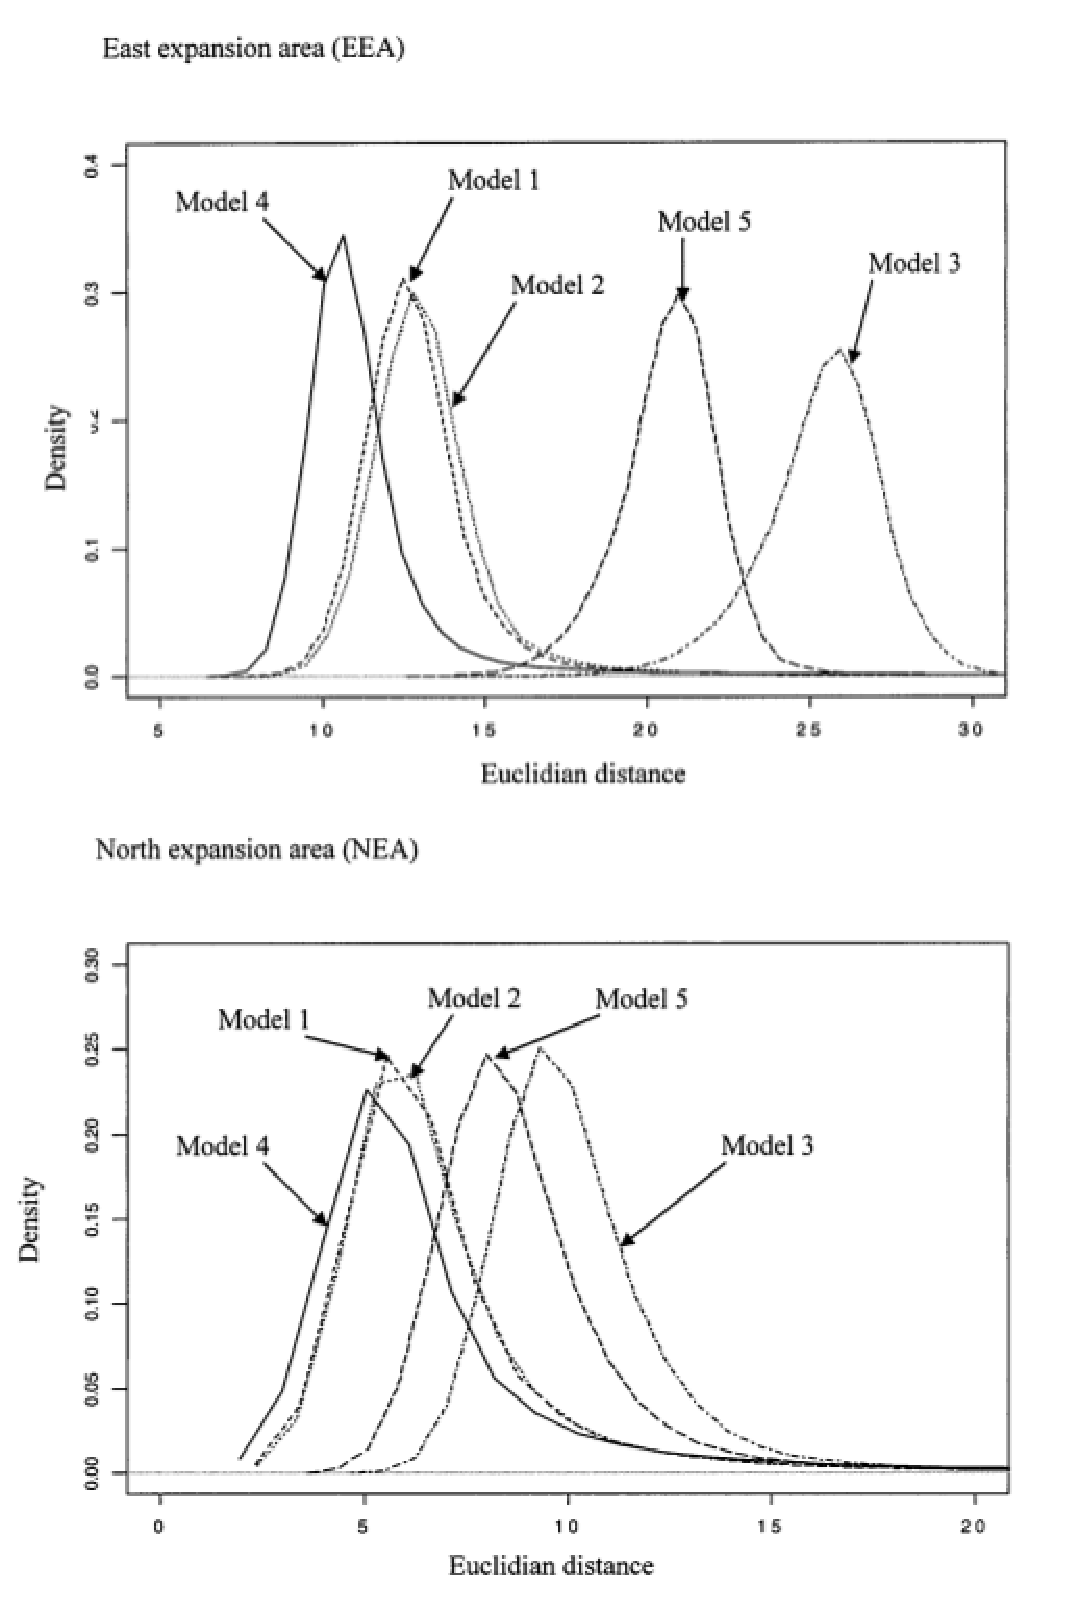
\includegraphics[width=4.5in]{cane-toad-models.eps}
\end{center}
\caption{Posterior distribution of $\delta$ for the five models
  considered in Estoup et al.~\cite{Estoup-etal-2004}.}\label{fig:cane-toad-models}
\end{figure}

Of course, we also have estimates for various parameters associated
with this model: 

\begin{itemize}

\item $N_{e_s}$: the effective population size when the population is
  stable.

\item $N_{e_f}$: the effective population size when a new population
  is founded.

\item $F_R$: the founding ratio, $N_{e_s}/N_{e_f}$.

\item $m$: the migration rate.

\item $N_{e_s}m$: the effective number of migrants per generation.

\end{itemize}

The estimates are summarized in Table~\ref{table:cane-toad}. Although
the credible intervals are fairly broad,\footnote{And notice that
  these are 90\% credible intervals, rather than the conventional 95\%
  credible intervals, which would be even broader.} there are a few
striking features that emerge from this analysis.

\begin{itemize}

\item Populations in the northern expansion area are larger, than
  those in the eastern expansion region. Estoup et
  al.~\cite{Estoup-etal-2004} suggest that this is consistent with
  other evidence suggesting that ecological conditions are more
  homogeneous in space and more favorable to cane toads in the north
  than in the east.

\item A smaller number of individuals is responsible for founding new
  populations in the east than in the north, and the ratio of
  ``equilibrium'' effective size to the size of the founding
  population is bigger in the east than in the north. (The second
  assertion is only weakly supported by the results.)

\item Migration among populations is more limited in the east than in
  the north. 

\end{itemize}

As Estoup et al.~\cite{Estoup-etal-2004} suggest, results like these
could be used to motivate and calibrate models designed to predict the
future course of the invasion, incorporating a balance between gene
flow (which can reduce local adaptation), natural selection, drift,
and colonization of new areas.

\begin{table}
\begin{center}
\begin{tabular}{ccr}
\hline\hline
Parameter & area & mean (5\%, 90\%) \\
\hline
$N_{e_s}$ & east & 744 (205, 1442) \\
         & north & 1685 (526, 2838) \\
$N_{e_f}$ & east & 78 (48, 118) \\
         & north & 311 (182, 448) \\
$F_R$    & east & 10.7 (2.4, 23.8) \\
         & north & 5.9 (1.6, 11.8) \\
$m$      & east & 0.014 ($6.0 \times 10^{-6}$, 0.064) \\
         & north & 0.117 ($1.4 \times 10^{-4}$, 0.664) \\
$N_{e_s}m$ & east & 4.7 (0.005, 19.9) \\
          & north & 188 (0.023, 883) \\
\hline
\end{tabular}
\end{center}
\caption{Posterior means and 90\% credible intervals for parameters of
  model 4 in the eastern and northern expansion areas of {\it Bufo
    marinus}.}\label{table:cane-toad}
\end{table}

\section*{Limitations of ABC}\index{Approximate Bayesian Computation!limitations}

If you've learned anything by now, you should have learned that there
is no perfect method. An obvious disadvantage of ABC relative to
either {\tt Migrate} or {\tt IMa2} is that it is much more
computationally intensive. 

\begin{itemize}

\item Because the scenarios that can be considered are much more
  complex, it simply takes a long time to simulate all of the data. 

\item In the last few years, one of the other disadvantages{\dash}that
  you had to know how to do some moderately complicated scripting to
  piece together several different packages in order to run
  analysis{\dash}has become less of a problem. {\tt popABC}
  (\url{http://code.google.com/p/popabc/}, {\tt DIYABC}
  (\url{http://www1.montpellier.inra.fr/CBGP/diyabc/}), and the {\tt
    abc\/} library in {\tt R} make it {\it relatively\/}
  easy\footnote{Emphasis on ``relatively''.} to perform the
  simulations.

\item Selecting an appropriate set of summary statistics isn't easy,
  and it turns out that which set is most appropriate may depend on
  the value of the parameters that you're trying to estimate and the
  which of the scenarios that you're trying to compare is closest to
  the actual scenario applying to the populations from which you
  collected the data. Of course, if you knew what the parameter values
  were and which scenario was closest to the actual scenario, you
  wouldn't need to do ABC in the first place.

\item In the end, ABC allows you to compare a small number of
  evolutionary scenarios. It can tell you which of the scenarios
  you've imagined provides the best combination of fit to the data and
  parsimonious use of parameters (if you choose model comparison
  statistics that include both components), but it takes additional
  work to determine whether the model is adequate, in the sense that
  it does a good job of explaining the data. Moreover, even if you
  determine that the model is adequate, you can't exclude the
  possibility that there are other scenarios that might be equally
  adequate{\dash}or even better.

\end{itemize}

\bibliography{popgen}
\bibliographystyle{plain}

\ccLicense

\end{document}

\chapter{Statistical phylogeography: Admixture graphs and {\tt sparg}}

Pickrell and Pritchard~\cite{Pickrell-Pritchard-2012} described the
most widely used approach to estimating admixture graphs. It is
implemented in {\tt TreeMix}.\index{TreeMix} At about the same time
Patterson et al.~\cite{Patterson-etal-2012} described a related method
at about the same time. I'm going to focus on the {\tt TreeMix}
approach because I am more comfortable with the underlying
model.\footnote{If you're curious about why I'm more comfortable with
  the Pickrell and Pritchard approach, feel free to ask.}
Unfortunately, if you want to use {\tt TreeMix}, you'll have to be comfortable
with compiling C++ programs from source~(or find a friend who can help
you or who can share a copy).\footnote{The most recent version of the
  {\tt TreeMix} manual notes that ``TreeMix should run on any Unix or
  Unix-like (e.g., Linux or Mac OS X) system. It may be more difficult
  to get it compiled under Windows. Notice that regardless of
  operating system, you'll also need to install the GNU Scientific
  Library and the Boost Graph Library.''}

The basic idea between {\tt Treemix} is not too complicated, although
it would be a stretch to say that it's simple. We start by assuming
that the allele frequencies are changing as a result of genetic
drift. Results going back to Kimura~\cite{Kimura-1955} tell us that
the variance in allele frequency is
\[
  \mbox{Var}(p_t) = p_o(1-p_0)\left(1 - e^{-t/2N_e}\right) \quad ,
\]
where $p_t$ is the allele frequency in the population at time $t$,
$p_o$ is the initial allele frequency, $t$ is the number of
generations, and $N_e$ is the effective population size. So long as
the effective population size is large enough that allele frequency
changes are relatively small from generation to generation and so long
as $p_o$ is not ``too close'' to 0 or 1, then we can approximate the
probability distribution of allele frequencies at time $t$ with a
normal distribution:
\[
  \mbox{P}(p_t|p_o,t,N_e) \sim \mbox{N}\left(p_o,
    p_o(1-p_o)\left(\frac{t}{2N_e}\right)\right) \quad .
\]
Now suppose we have a series of four populations related like those
shown in Figure~\ref{fig:treemix-no-migration}. As you can see, this
example shows populations that have a simple tree-like
relationship. Here's where the fun starts.

\begin{figure}
  \begin{center}
    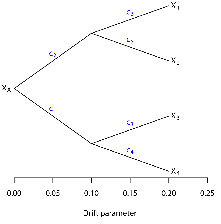
\includegraphics[width=12cm]{treemix-no-migration.eps}
  \end{center}
  \caption{A purely tree-like relationship among four hypothetical
    populations. The allele frequencies in each population are
    represented by $X_i$. The drift parameter on the $x$-axis is $t/2N_e$,
    i.e., it's measuring time from the root of the tree to the tips in
    units of $1/2N_e$. A part of a figure in~\cite{Pickrell-Pritchard-2012}.}\label{fig:treemix-no-migration}
\end{figure}

It's a well known fact~\cite{CavalliSforza-Edwards-1967} that the
variance in allele frequencies ($X_i$ in the figure) are simply
\begin{eqnarray*}
  \mbox{Var}(X_1) &=& (c_2 + c_6)X_A(1-X_A) \\
  \mbox{Var}(X_2) &=& (c_2 + c_5)X_A(1-X_A) \\
  \mbox{Var}(X_3) &=& (c_1 + c_3)X_A(1-X_A) \\
  \mbox{Var}(X_4) &=& (c_1 + c_4)X_A(1-X_A) \quad ,
\end{eqnarray*}
where $c_i = \frac{t_i}{2N_e^{(i)}}$, $t_i$ is the time associated
with branch $i$ and $N_e^{(i)}$ is the effective size of the
population associated with branch $i$. It's obvious from looking at
the tree that populations 1 and 2 have been evolving independently
from populations 3 and 4 from the start, while 1 and 2 have been
evolving independently of one another for a shorter period of time. As
a result, we expect allele frequencies in pouplations 1 and 2 to be
more similar than those in populations 3 and 4. In fact, Pickrell and
Pritchard point out that we can write the various covariances down
pretty simply too:
\begin{eqnarray*}
  \mbox{Cov}(X_1,X_2) &=& c_2X_A(1-X_A) \\
  \mbox{Cov}(X_1,X_3) &=& 0 \\
  \mbox{Cov}(X_1,X_4) &=& 0 \\
  \mbox{Cov}(X_2,X_3) &=& 0 \\
  \mbox{Cov}(X_2,X_4) &=& 0 \\
  \mbox{Cov}(X_3,X_4) &=& c_1X_A(1-X_A) \quad .
\end{eqnarray*}
As a result, we can write down a multivariate probability distribution
that describes all of the allele frequencies simultaneously, given the
same caveats as above about the normal distribution.
\[
  \mbox{P}(\bf p_t|\bf p_0, \bf t, \bf N_e) \sim \mbox{MVN}(\bf p_0,
  \bf \Sigma) \quad ,
\]
where boldface refers to vectors, MVN refers to the multivariate
normal distribution, and $\bf Sigma$ is the covariance matrix of
allele frequencies. Since we can write down that probability
distribution, you can probably imagine that it's possible to estimate
the likelihood of our data given a particular tree. To get a maximum
likelihood estimate of how our populations are related, assuming
there's no migration, we simply have to compare the likelihoods across
all possible trees and choose the one that's most likely.\footnote{If
  you know anything about estimating phylogenies, you know there is
  tremendous complexity buried in that ``simply have to compare.''
  Also notice that if we can get a maximum likelihood estimate, we can
  also get a full Bayesian posterior ``simply'' by providing the
  appropriate priors.}

Now suppose we allow migration from one of our populations into
another. The simple example Pickrell and Pritchard
provide~(Figure~\ref{fig:treemix-figure} shows a single migration from
the lineage leading to population 2 into population 3, labeling the
source population as $Y$ and the destination population as $Z$. As you
can see in Panel D of the figure, the migration event changes the
structure of the covariance matrix. Since all the migration event does
is to change the covariance matrix, we can once again explore
parameter space and find the network that maximizes the
likelihood. When we do so, not only do we have estimates for
population relationships and effective population sizes but also for
the timing and direction of migration events. Estimating admixture is,
however, even more challenging than estimating a population
phylogeny. The number of alternative configurations explodes rapidly
with more than 4-5 populations, making heuristic searches
necessary. Molloy et al.~\cite{Molloy-etal-2021} recently described a
new approach that builds on {\tt TreeMix} and seems to avoid getting
stuck in a local optimum. Since the basic approach is the same and
this isn't a course in computational biology, we won't discuss it
further, but you should investigate it if you use admixture graphs in
any of your work.

\begin{figure}
  \begin{center}
    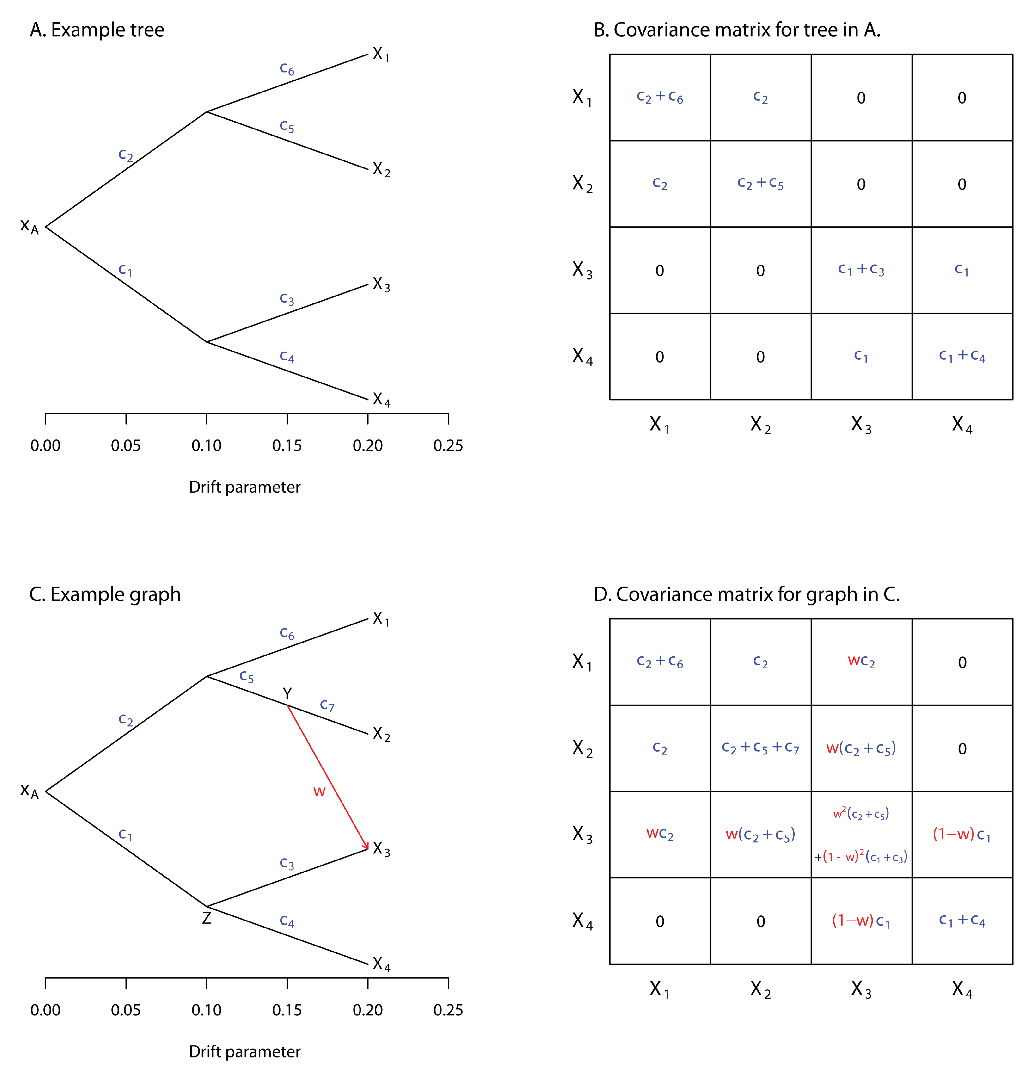
\includegraphics[width=14cm]{treemix-figure.eps}
  \end{center}
  \caption{Illustrating the covariance matrices of admixed and
    unadmixed populations. From \cite{Pickrell-Pritchard-2012}.}\label{fig:treemix-figure}
\end{figure}

\section*{Estimating dispersal and ancestral
  geography}\index{ancestral geography}\index{sparg@{\tt sparg}}

As you can see, admixture graphs provide a very flexible approach to
understanding the history of populations. But they do have one
significant limitation. We have to know ahead of time which
indivdiuals belong in which populations, just as we did with
$F$-statistics,\index{F-statistics@$F$-statistics} and just as with
{\tt STRUCTURE} gave us a way to look at population structure without
pre-assigning individuals to populations, there's a way of looking at
ancestry that uses individuals rather than pre-defined
populations~\cite{Osmond-Coop-2021}. As with admixture graphs, the
mathematics lying behind the approach gets pretty hairy, but the basic
idea is pretty simple~(Figure~\ref{fig:sparg-overview}).

\begin{figure}
  \begin{center}
    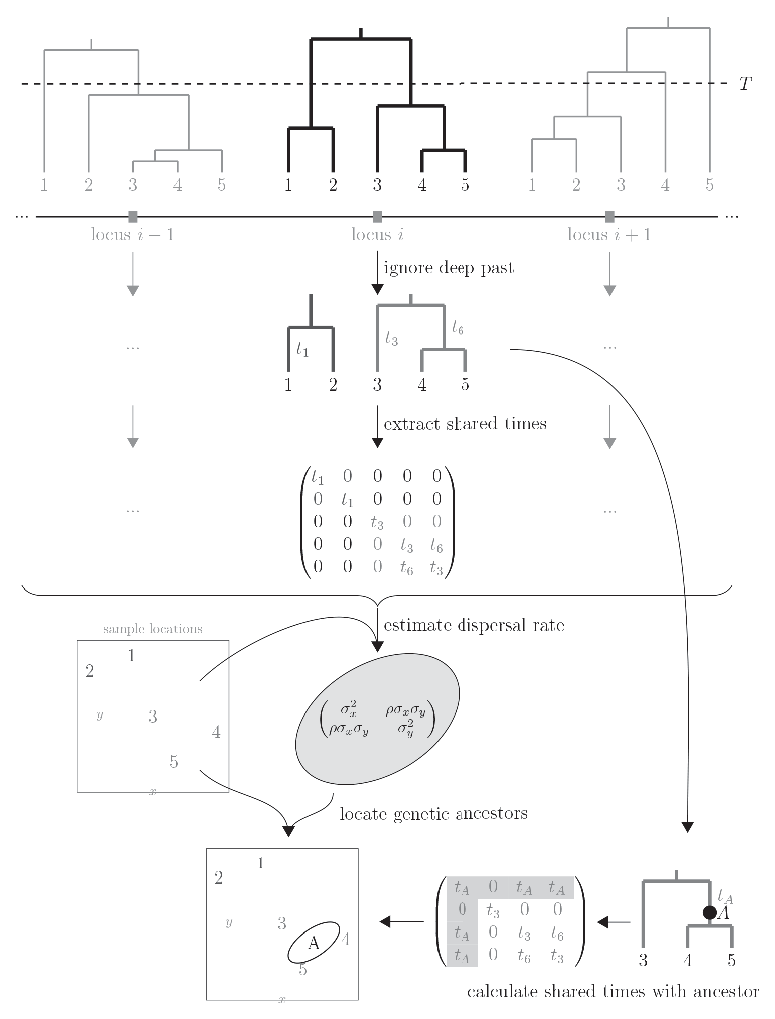
\includegraphics[width=14cm]{sparg-overview.eps}
  \end{center}
  \caption{Conceptual overview of the process for estimating the
    spatial position of ancestors
    (from~\cite{Osmond-Coop-2021}).}\label{fig:sparg-overview} 
\end{figure}

\begin{itemize}

  \item At any position along a genome, we can construct a
    phylogeneitc tree showing the genealogical relationship among all
    chromosomes in the sample at that location.\footnote{Notice that I
      wrote ``chromosomes'', not individuals, because the different
      allele copies within an individual may have different
      genealogical histories.} 

  \item Individuals disperse randomly through space with the distance
    of an offspring from its mother given by a bivariate normal
    distribution with a mean of 0 and a covariance matrix
    $\bf\Sigma$. In any real sample, glacial migrations,
    barriers to dispersal, or the opening of new habitat will cause
    some aspects of the dispersal history not to be well approximated
    by this model of Brownian motion, so we only use parts of the tree
    from the first step that are more recent than these events to
    estimate dispersal parameters.\footnote{Notice that while this
      approach means that the Brownian motion model for disperal is a
      better fit to the data, it also means that we can't use this
      approach to study events that involve ancient dispersal, like
      early modern human movemeents out of Africa.}

  \item Given the estimates of time to a common ancestor between two
    individuals, the spatial location of those individuals, and the
    dispersal rate, we can estimate the spatial location of the
    ancestor. 

\end{itemize}

This method implicitly assumes that differences are selectively
neutral.\footnote{Remember: This doesn't mean that there aren't any
  fitness differences, only that the product of the selection
  coefficient associated with any of those differences and the
  population size is less than one, implying that the evolutionary
  dynamics are rougly similar to those of a purely neutral locus.}
Although we could try this approach with data from only one locus, the
results are unlikely to be informative for two reasons. First, there
is a lot of uncertainty associated with our estimate of phylogenetic
relationships at one locus. Second, because the coalescent history of
unlinked loci will differ even though the effective population size
and the patterns of migration that affect different loci are the
same. But since the patterns of migration {\it are\/} the same across
different loci and since the effective population size {\it is\/} the
same across loci, we can combine information across loci to get better
estimates of the dispersal rates. Since we estimate the location of
ancestors at every locus, we end up with a distribution of ancestral
locations rather than a single estimate. Osmond and Coop also point
out that we can define different ``epochs'' in which to estimate
dispersal rates and ancestors. This allows the dispersal rate to vary
over time. All of this is available in a Python package, {\tt sparg},
which should run on any platfrom with
phython3~(\url{https://github.com/mmosmond/sparg}).

\subsection*{An example from {\it Arabidopsis}}\index{Arabidopsis@{\it Arabidopsis thaliana}} 

Plant geneticists have studied {\it Arabidopsis thaliana\/}
extensively. Alonso-Blanco et al.~\cite{AlonsoBlanco-etal-2016}
reported results derived from sequencing 1135 different wild
accessions derived from Eurasia and North Africa. Osmond and Coop used
{\tt sparg} to explore historical patterns of disperal and the
geographical location of ancestors using this data set. They first
estimated dispersal rates in both a one-epoch model and in multi-epoch
models. As you can see in Figure~\ref{fig:arabidopsis-epochs}), the
estimates of dispersal rates are very similar across all of the
loci. In addition, the per-generation rate of east-west dispersal
($\sigma^2_{long}$) is about 10 times higher than north-sourth
dispersal ($\sigma^2_{lat}$), and the correlation between the two
rates ($\rho$) is relatively small. Comparison among the scenarios
suggests that the 4-epoch model is the best fit to the data,
suggesting that the rate of dispersal in the last 10 generations is
substantially greater than it was earlier and that dispersal between
10 and 1000 generations ago is greater than it was more than 1000
generations ago.

\begin{figure}
  \begin{center}
    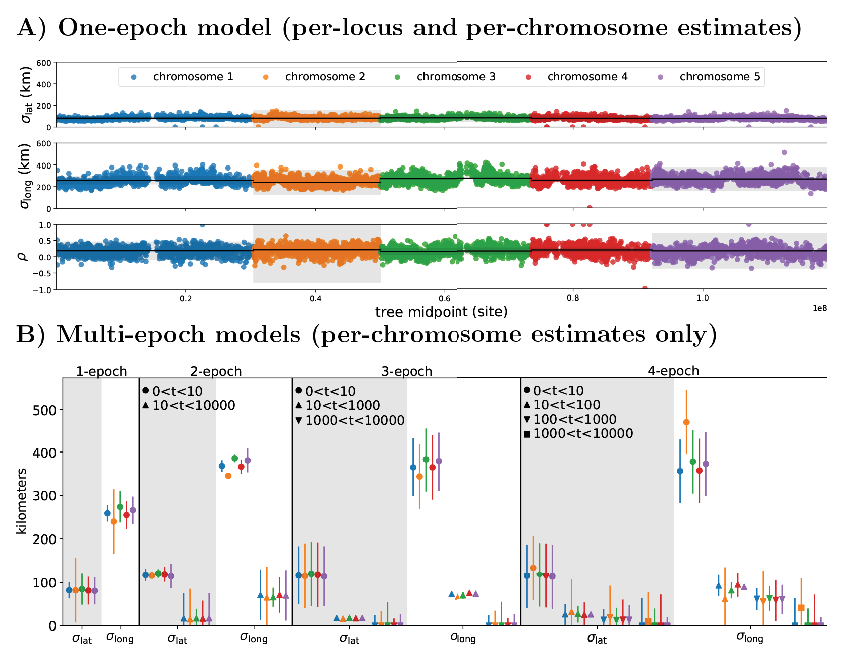
\includegraphics[width=14cm]{arabidopsis-epochs.eps}
  \end{center}
  \caption{Estimates of dispersal rates in {\it Arabidopsis
      thaliana\/} in both one-epoch (panel A) and multi-epoch (panel
    B) models (from~\cite{Osmond-Coop-2021}).}\label{fig:arabidopsis-epochs}
\end{figure}

Now that we have a good idea {\it when\/} dispersal happened, let's
see {\it where\/} it happened. As you can see in
Figure~\ref{fig:arabidopsis-dispersal}, much of the estimated
dispersal over the last 10-100 generations didn't move individuals
very far. In addition, it's a little hard to see, but if you zoom in
on the figure and focus on the purple colors, you'll notice that most
of the lines leading from the dots~(current locations) point towards
the center of Europe. This pattern is particularly clear in for the
100-generation ago ancestral location of samples from
Scandinavia. There are, however, a few individuals that moved very
long distances. Individual 9627, for example, seems to have an ancestor 10
generations ago that was more than 3000km to the east of its current
location, and its ancestor seems to have been more than 4000km to the
east 100 generations ago.

\begin{figure}
  \begin{center}
    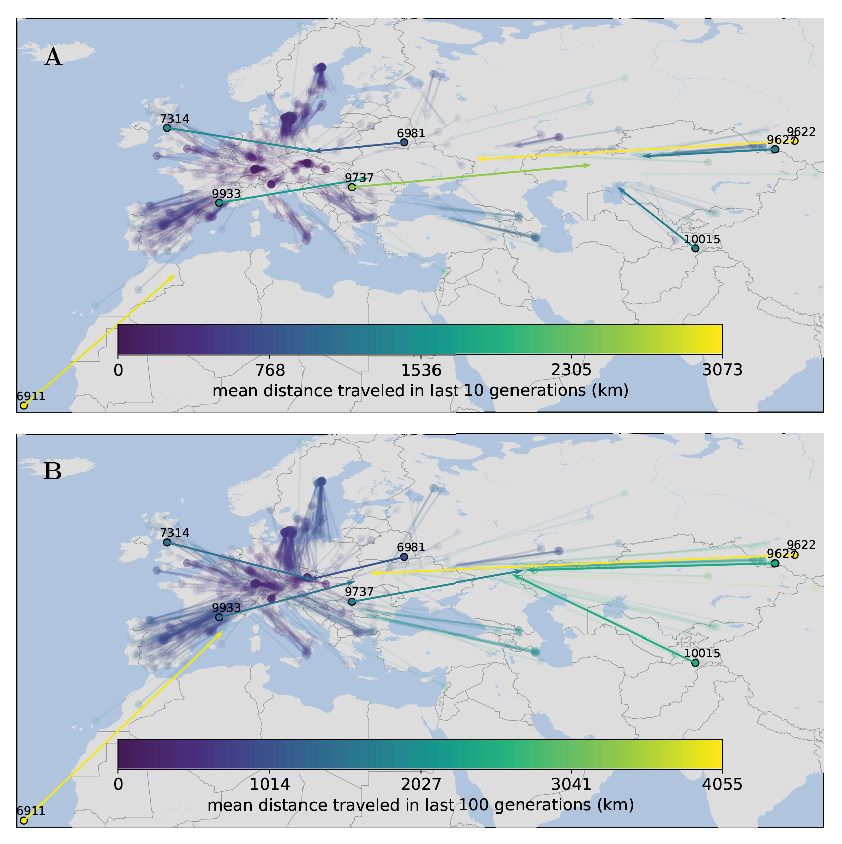
\includegraphics[width=14cm]{arabidopsis-dispersal.eps}
  \end{center}
  \caption{Estimates of the ancestral location of {\it Arabidopsis
      thaliana\/} accessions 10 and 100 generations ago
    (from~\cite{Osmond-Coop-2021}).}\label{fig:arabidopsis-dispersal}
\end{figure}


\chapter{Population genomics}

In the past decade, the development of high-throughput methods for
genomic sequencing (next-generation sequencing: NGS) have
revolutionized how many geneticists collect data. It is now possible
to produce so much data so rapidly that simply storing and processing
the data poses great challenges~\cite{Nekrutenko-Taylor-2012}. The
Nekrutenko and Taylor review~\cite{Nekrutenko-Taylor-2012} doesn't
even discuss the new challenges that face population geneticists and
evolutionary biologists as they start to take advantage of those
tools, nor did it discuss the promise these data hold for providing
new insight into long-standing questions, but the challenges and the
promise are at least as great as those they do
describe.\index{next-generation sequencing}

To some extent the most important opportunity provided by NGS
sequencing is simply that we now have a lot more data to answer the
same questions. For example, using a technique like RAD
sequencing~\cite{Baird-etal-2008} or genotyping-by-sequencing
(GBS:~\cite{Elshire-etal-2011}), it is now possible to identify
thousands of polymorphic SNP markers in non-model organisms, even if
you don't have a reference genome available. As we've seen several
times this semester, the variance associated with drift is
enormous. Many SNPs identified through RAD-Seq or GBS are likely to be
independently inherited. Thus, the amount and pattern of variation at
each locus will represent an independent sample from the underlying
evolutionary process. As a result, we should be able to get much
better estimates of fundamental parameters like $\theta=4N_e\mu$,
$M=4N_em$, and $R=4N_er$ and to have much greater power to
discriminate among different evolutionary scenarios. Willing et
al.~\cite{Willing-etal-2012}, for example, present simulations
suggesting that accurate estimates of $F_{ST}$ are possible with
sample sizes as small as 4--6 individuals per population, so long as
the number of markers used for inference is greater than
1000.\index{RAD sequencing}\index{next-generation sequencing!estimating $F_{ST}$}\index{genotyping-by-sequencing}

\section*{A quick overview of NGS methods}

I won't review the chemistry used for next-generation sequencing. It
changes very rapidly, and I can't keep up with it. Suffice it to say
that 454 Life Sciences, Illumina, PacBio, and probably other companies
I don't know about each have different approaches to very high
throughput DNA sequencing. What they all have in common is that the
whole genome is broken into small fragments and sequnced and that a
single run through the machine produces an enormous amount of data,
134-6000 Gb and up to 20 billion readsfrom a NovaSeq 600 for
example~(\url{https://www.illumina.com/systems/sequencing-platforms/comparison-tool.html};
accessed 30 December 2018).\footnote{In NGS applications for
  phylogeny, a strategy of targeted enrichment is often used. In this
  approach, pre-identified parts of the genome are ``baited'' using
  primers and those parts of the genome are enriched through PCR
  before the sequencing library is
  constructed~\cite{Lemmon-etal-2012}. By the way, when I taught this
  course two years ago the Illumina HiSeq X Ten produced the most data
  from a single run, up to 1800 Gb and 3-6 billion reads. That means
  the volume of sequence you can produce in a single run has tripled
  in two years.}

\subsection*{RAD sequencing}\index{RAD sequencing}

Baird et al.~\cite{Baird-etal-2008} introduced RAD a little over a
decade ago. One of its great attraction for evolutionary geneticists
is that RAD-seq can be used in any organism from which you can extract
DNA and the laboratory manipulations are relatively straightforward.

\begin{itemize}

\item Digest genomic DNA from each individual with a restriction
  enzyme, and ligate an adapter to the resulting fragments. The
  adapter includes a forward amplification primer, a sequencing primer
  and a ``barcode'' used to identify the individual from which the DNA
  was extracted.

\item Pool the individually barcoded samples~(``normalizing'' the
  mixture so that roughly equal amounts of DNA from each individual
  are present) shear them and select those of a size appropriate for
  the sequencing platform you are using.

\item Ligate a second adapter to the sample, where the second adapter
  is the reverse complement of the reverse amplification primer. 

\item PCR amplification will enrich only DNA fragments having both the
  forward and reverse amplification primer.

\end{itemize}

\noindent The resulting library consists of sequences within a
relatively small distance from restriction sites.

\subsection*{Genotyping-by-sequencing}\index{genotyping-by-sequencing}

Genotyping-by-sequencing~(GBS) is a similar approach. 

\begin{itemize}

\item Digest genomic DNA with a restriction enzyme and ligate two
  adapters to the genomic fragments. One adapter contains a barcode
  and the other does not.

\item Pool the samples.

\item PCR amplify and sequence. Not all ligated fragments will be
  sequenced because some will contain only one adapter and some
  fragments will be too long for the NGS platform.

\end{itemize}

\noindent Once an investigator has her sequenced fragments back, she
can either map the fragments back to a reference genome or she can
assemble the fragments into orthologous sequences {\it de novo}. I'm
not going to discuss either of those processes, but you can imagine
that there's a lot of bioinformatic processing going on. What I want
to focus on is what you do with the data and how you interpret it.

\section*{Next-generation phylogeography}\index{next-generation sequencing!phylogeography}

The American pitcher plant mosquito {\it Wyeomyia
  smithii\/} has been extensively studied for many years. It's a model
organism for ecology, but its genome has not been sequenced. An
analysis of {\it COI} from 20 populatins and two outgroups produced
the set of relationships you see in
Figure~\ref{fig:wyeomyia-COI}~\cite{Emerson-etal-2010}.\index{Wyeomyia@\textit{Wyeomyia}!\textit{smithii}}
As you can see, this analysis allows us to distinguish a northern
group of populations from a southern group of populations, but it
doesn't provide us any reliable insight into finer scale
relationships. 

\begin{figure}
\begin{center}
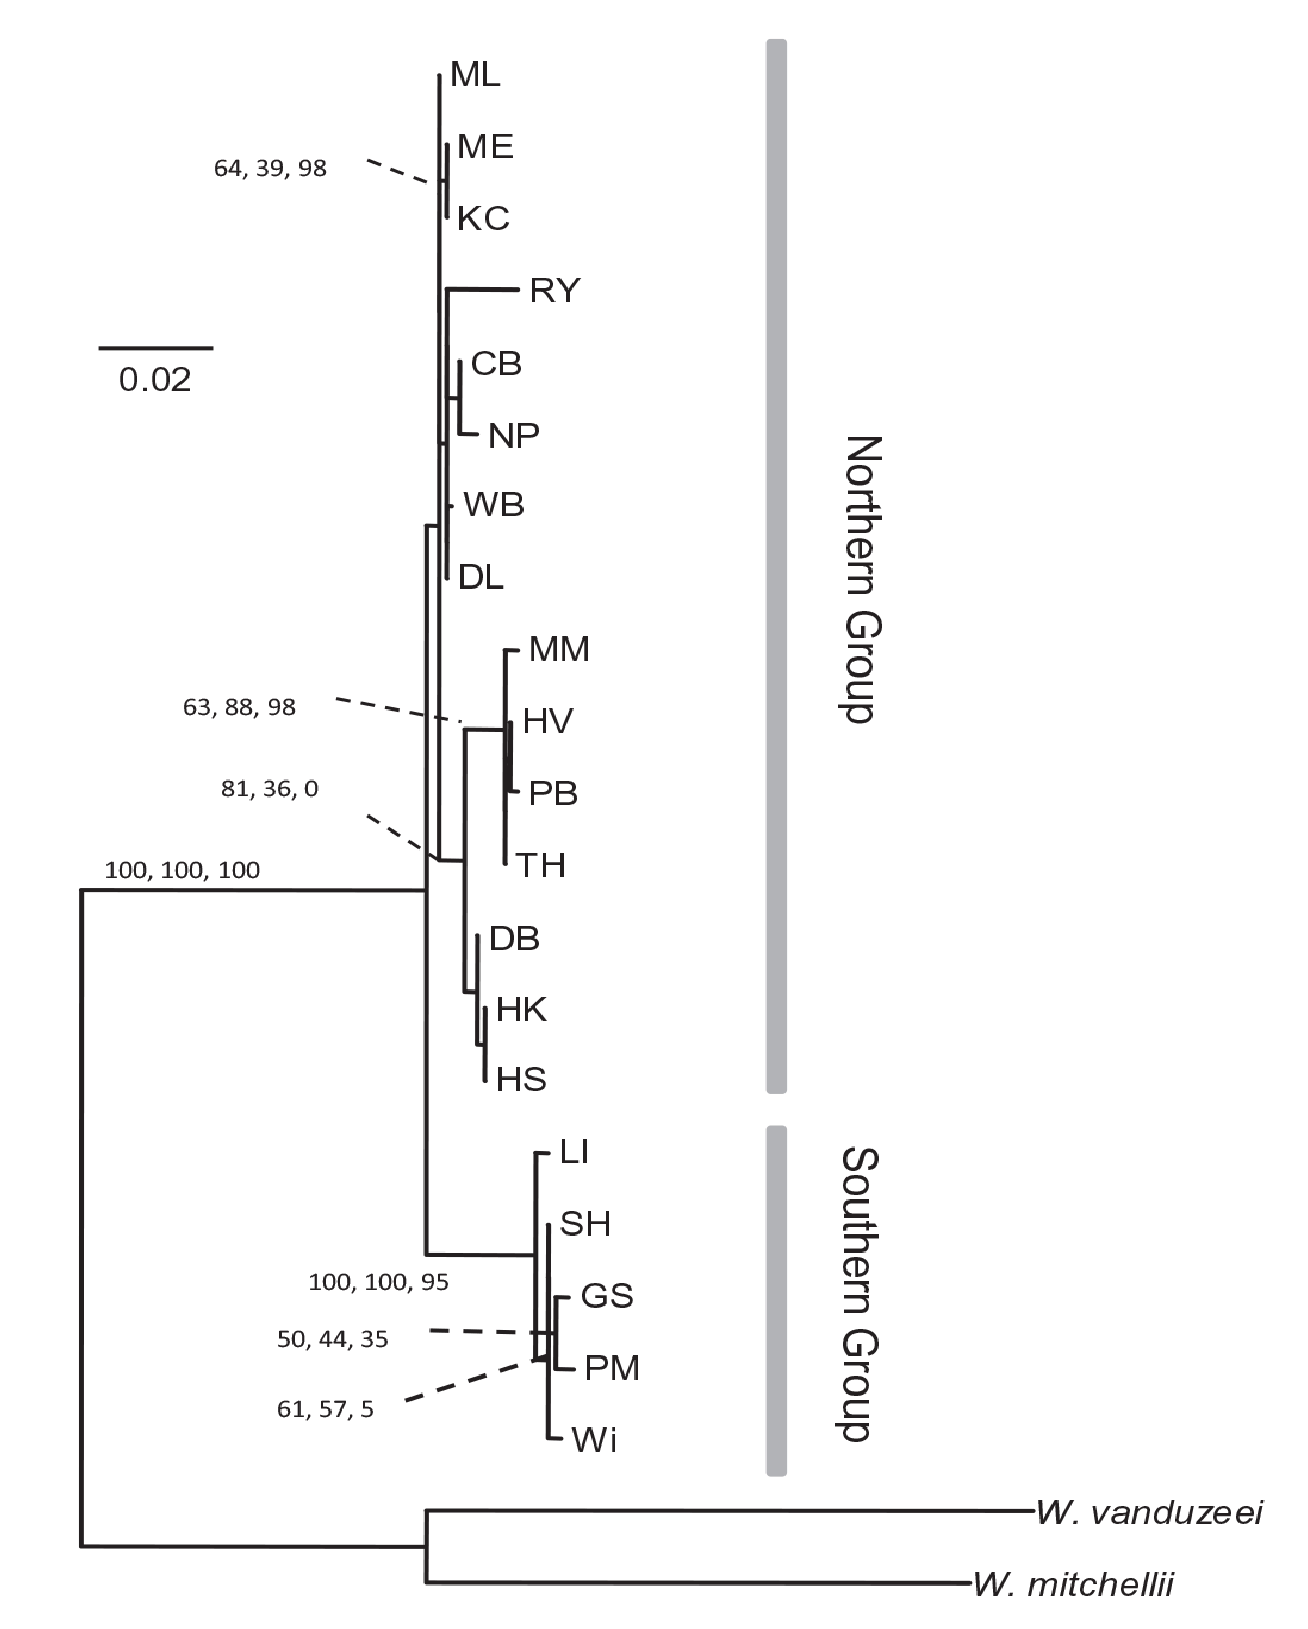
\includegraphics[width=0.9\textwidth]{wyeomyia-COI.eps}
\end{center}
\caption{Maximum-likelihood phylogenetic tree depicting relationshps
  among populations of {\it W. smithii\/} relative to the outgroups
  {\it W. vanduzeei\/} and {\it W. mitchelli} (from~\cite{Emerson-etal-2010}).}\label{fig:wyeomyia-COI}
\end{figure}

Using the same set of samples, the authors used RAD sequencing to
identify 3741 SNPs. That's more than 20 times the number of variable
sites found in {\it COI}, 167. Not surprisingly, the large number of
additional sites allowed the authors to produce a much more highly
resolved phylogeny~(Figure \ref{fig:wyeomyia-RAD}). With this
phylogeny it's easy to see that southern populations are divided into
two distinct groups, those from North Carolina and those from the Gulf
Coast. Similarly, the northern group of populations is subdivided into
those from the Appalachians in North Carolina, those from the
mid-Atlantic coast, and those from further north. The glacial history
of North America means that both the mid-Atlantic populations and the
populations farther north must have been derived from one or more
southern populations after the height of the last glaciation. Given
the phylogenetic relationships recovered here, it seems clear that
they are most closely related to populations in the Appalachians of
North Carolina.

\begin{figure}
\begin{center}
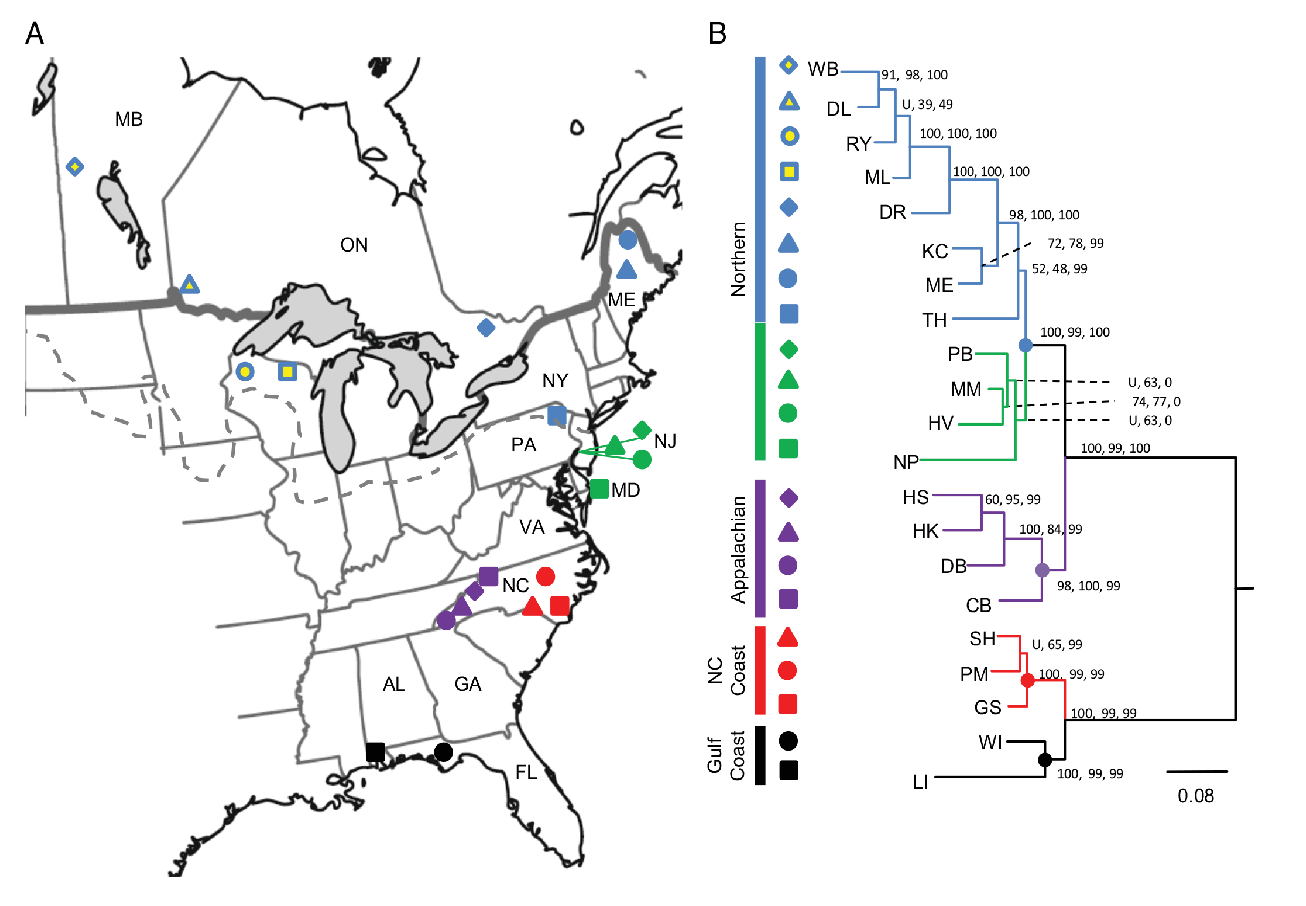
\includegraphics[width=0.9\textwidth]{wyeomyia-RAD.eps}
\end{center}
\caption{A. Geographical distribution of samples included in the
  analysis. B. Phylogenetic relationship of samples included in the analysis.}\label{fig:wyeomyia-RAD}
\end{figure}

That's the promise of NGS for population genetics. What are the
challenges? Funny you should ask.

\section*{Estimates of nucleotide diversity\footnote{This section draws heavily on~\cite{Lynch-2008}}}\index{next-generation sequencing!estimating nucleotide diversity}

Beyond the simple challenge of dealing with all of the short DNA
fragments that emerge from high-throughput sequencing, there are at
least two challenges that don't arise with data obtained in more
traditional ways.

\begin{enumerate}

\item Most studies involve ``shotgun'' sequencing of entire
  genomes. In large diploid genomes, this leads to variable
  coverage. At sites where coverage is low, there's a good chance that
  all of the reads will be derived from only one of the two
  chromosomes present, and a heterozygous individual will be scored as
  homozygous. ``Well,'' you might say, ``let's just throw away all of
  the sites that don't have at least 8$\times$ coverage.''\footnote{If
    both chromosomes have an equal probability of being sequenced, the
    probability that one of them is missed with 8$\times$ coverage is
    $(1/2)^8 = 1/256$.} That would work, but you would also be
  throwing out a lot of potentially valuable information.\footnote{It's
    valuable information, providing you know how to deal with in
    properly.} It seems better to develop an approach that lets us use
  {\it all\/} of the data we collect.

\item Sequencing errors are more common with high-throughput methods
  than with traditional methods, and since so much data is produced,
  it's not feasible to go back and resequence apparent polymorphisms
  to see if they reflect sequencing error rather than real
  differences. Quality scores can be used, but they only reflect the
  quality of the reads from the sequencing reaction, not errors that
  might be introduced during sample preparation. Again, we might focus
  on high-coverage sites and ignore ``polymorphisms'' associated with
  single reads, but we'd be throwing away a lot of
  information.

\end{enumerate}
A better approach than setting arbitrary thresholds and throwing away
data is to develop an explicit model of how errors can arise during
sequencing and to use that model to interpret the data we've
collected. That's precisely the approach that Lynch~\cite{Lynch-2008}
adopts. Here's how it works assuming that we have a sample from a
single, diploid individual:

\begin{itemize}

\item Any particular site will have a sequence profile, $(n_1, n_2,
  n_3, n_4)$, corresponding to the number of times an A, C, G, or T
  was observed. $n=n_1+n_2+n_3+n_4$ is the depth of coverage for that
  site. 

\item Let $\epsilon$ be the probability of a sequencing error at any
  site, and assume that all errors are equiprobable, e.g., there's no
  tendency for an A to be miscalled as a C rather than a T when it's
  miscalled.\footnote{It wouldn't be hard, conceptually, to allow
    different nucleotides to have different error rates, e.g.,
    $\epsilon_A$, $\epsilon_C$, $\epsilon_G$, $\epsilon_T$, but the
    notation would get really complicated, so we won't bother trying
    to show how differential error rates can be accommodated.} 

\item If the site in question were homozygous A, the probability of
  getting our observed sequence profile is:
\[
P(n_1,n_2,n_3,n_4|\mbox{homozygous A},\epsilon)
=
{n \choose n_1}(1-\epsilon)^{n_1}\epsilon^{n-n_1} \quad .
\]
A similar relationship holds if the site were homozygous C, G, or
T. Thus, we can calculate the probability of our data if it were homozygous
as\footnote{This expression
    looks a little different from the one in~\cite{Lynch-2008}, but
    I'm pretty sure it's equivalent.}
\[
P(n_1,n_2,n_3,n_4|\mbox{homozygous},\epsilon)
=
\sum_{i=1}^4 \left(\frac{p_i^2}{\sum_{j=1}^4p_j^2}\right) 
{n \choose n_i}(1-\epsilon)^{n_i}\epsilon^{n-n_i}
\quad .
\]

\item If the site in question were heterozygous, the probability of
  getting our observed sequence profile is a bit more complicated. Let
  $k_1$ be the number of reads from the first chromosome and $k_2$ be
  the number of reads from the second chromosome ($n=k_1+k_2$). Then
\begin{eqnarray*}
P(k_1,k_2)
&=&
{n \choose k_1}\left(\frac{1}{2}\right)^{k_1}
               \left(\frac{1}{2}\right)^{k_2}
\\
&=&
{n \choose k_1}\left(\frac{1}{2}\right)^n \quad .
\end{eqnarray*}
Now consider the ordered genotype $x_ix_j$, where $x_i$ refers to the
nucleotide on the first chromosome and $x_j$ refers to the nucleotide
on the second chromosome. The probability of getting our observed
sequence profile from this genotype given that we have $k_1$ reads
from the first chromosome and $k_2$ reads from the second is:
{\footnotesize
\begin{eqnarray*}
P(n_1,n_2,n_3,n_4|x_i,x_j,k_1,k_2)
&=&
\sum_{l=1}^4\sum_{m=0}^{k_1}{k_1 \choose m}(1-\delta_{il})^m\delta_{il}^{k_1-m}
{k_2 \choose n_i-m}(1-\delta_{jl})^{n_1-m}\delta_{jl}^{k_2-(n_1-m)}
\quad ,
\end{eqnarray*}
}
where 
\[
\delta_{il} = \left\{\begin{array}{ll}
1-\epsilon & \mbox{if } i = l \\
\epsilon & \mbox{if } i \ne l \quad .
\end{array}
\right.
\]
We can use Bayes' Theorem\footnote{Ask me for details if you're
  interested.} to get
\[
P(n_1,n_2,n_3,n_4|x_i,x_j,\epsilon) =
P(n_1,n_2,n_3,n_4|x_i,x_j,k_1,k_2,\epsilon)P(k_1,k_2) \quad ,
\]
and with that in hand we can get
\[
P(n_1,n_2,n_3,n_4|\mbox{heterozygous},\epsilon)
=
\sum_{i=1}^4\sum_{j\ne i}
\left(\frac{x_ix_j}{1-{\sum_{l=1}^4p_l^2}}\right) P(n_1,n_2,n_3,n_4|x_i,x_j,\epsilon) 
\]

\item Let $\pi$ be the probability that any site is heterozygous. Then
  the probability of getting our data is:
{\footnotesize
\[
P(n_1,n_2,n_3,n_4|\pi,\epsilon)
=
\pi P(n_1,n_2,n_3,n_4|\mbox{heterozygous},\epsilon)
+
(1-\pi)P(n_1,n_2,n_3,n_4|\mbox{homozygous},\epsilon) \quad .
\]
}

\item What we've just calculated is the probability of the
  configuration we observed at a particular site. The probability of
  our data is just the product of this probability across all of the
  sites in our sample:
\[
P(\mbox{data}|\pi,\epsilon) = \prod_{s=1}^S
P(n_1^{(s)},n_2^{(s)},n_3^{(s)},n_4^{(s)}|\pi,\epsilon) \quad ,
\]
where the superscript $(s)$ is used to index each site in the data.

\item What we now have is the likelihood of the data in terms of
  $\epsilon$, which isn't very interesting since it's just the average
  sequencing error rate in our sample, and $\pi$, which is
  interesting, because it's the genome-wide nucleotide diversity. Now
  we ``simply'' maximize that likelihood, and we have
  maximum-likelihood estimates of both parameters. Alternatively, we
  could supply priors for $\epsilon$ and $\pi$ and use MCMC to get
  Bayesian estimates of $\epsilon$ and $\pi$.  

\end{itemize}

Notice that this genome-wide estimate of nucleotide diversity is
obtained from a sample derived from a single diploid
individual. Lynch~\cite{Lynch-2008} develops similar methods for
estimating gametic disequilibrium as a function of genetic distance
for a sample from a single diploid individual. He also extends that
method to samples from a pair of individuals, and he describes how to
estimate mutation rates by comparing sequences derived from
individuals in mutation accumulation lines with consensus
sequences.\footnote{Mutation accumulation lines are lines propagated
  through several (sometimes up to hundreds) of generations in which
  population sizes are repeatedly reduced to one or a few individuals,
  allowing drift to dominate the dynamics and alleles to
  ``accumulate'' with little regard to their fitness effects.}

Haubold et al.~\cite{Haubold-etal-2010} describe a program
implementing these methods. Recall that under the infinite sites model
of mutation $\pi = 4N_e\mu$. They analyzed data sets from the sea
squirt {\it Ciona intestinalis\/} and the water flea {\it Daphnia
  pulex}~(Table~\ref{table:NGS-results}). Notice that the sequencing
error rate in {\it D. pulex} is indistinguishable from the nucleotide
diversity.\index{Cionia@\textit{Cionia}!\textit{intestinalis}}\index{Daphnia@\textit{Daphnia}!\textit{pulex}}

\begin{table}
\begin{center}
\begin{tabular}{lccc}
\hline\hline
Taxon & $4N_e\mu$ & $4N_e\mu$ (low coverage) & $\epsilon$ \\
\hline
{\it Cionia intestinalis} & 0.0111 & 0.012 & 0.00113 \\
{\it Daphnia pulex} & 0.0011 & 0.0012 & 0.00121 \\
\hline
\end{tabular}
\end{center}
\caption{Estimates of nucleotide diversity and sequencing error rate
  in {\it Cionia intestinalis\/} and {\it Daphnia pulex}~(results
  from~\cite{Haubold-etal-2010}).}\label{table:NGS-results}
\end{table}

\section*{Next-generation AMOVA\footnote{This section depends heavily on~\cite{Gompert-Buerkle-2011}}}\index{next-generation sequencing!partitioning diversity}\index{BAMOVA}

What we've discussed so far gets us estimates of some population
parameters~($4N_e\mu$, $4N_er$), but they're derived from the
sequences in a single diploid individual. That's not much of a
population sample, and it certainly doesn't tell us anything about how
different populations are from one another. Gompert and
Buerkle~\cite{Gompert-Buerkle-2011} describe an approach to estimate
statistics very similar to $\Phi_{ST}$ from AMOVA. Since they take a
Bayesian approach to developing their estimates, they refer to
approach as BAMOVA, Bayesian models for analysis of molecular
variance. They propose several related models.

\begin{itemize}

\item {\bf NGS-individual model}: This model assumes that sequencing
  errors are negligible.\footnote{Or that they've already been
    corrected. We don't care {\it how\/} they might have been
    corrected. We care only that we can assume that the reads we get
    from a sequencing run faithfully reflect the sequences present on
    each of the chromosomes.} Under this model, the only trick is that
  we may or may not pick up both sequences from a heterozygote. The
  probability of not seeing both sequences in a heterozygote is
  related to the depth of coverage.

\item {\bf NGS-population model}: In some NGS experiments,
  investigators pool all of the samples from a population into a
  single sample. Again, Gompert and Buerkle assume that sequencing
  errors are negligible. Here we assume that the number of reads for
  one of two alleles at a particular SNP site in a sample is related
  to the underlying allele frequency at that site. Roughly speaking,
  the likelihood of the data at that site is then
\[
P(x_i|p_i,n_i, k_i) = {n_i \choose k_i}p_i^{k_i}(1-p_{i})^{n-k_i}
\quad ,
\]
where $p_i$ is the allele frequency at this site, $n_i$ is the sample
size, and $k_i$ is the count of one of the alleles in the sample. The
likelihood of the data is just the product across the site-specific
likelihoods.\footnote{The actual model they use is a bit more
  complicated than this, but the principles are the same.}

\end{itemize}

Then, as we did way back when we used a Bayesian appraach to estimate
$F_{ST}$~\cite{Holsinger-Wallace-2004}, we put a prior on the $p_i$
and the parameters of this prior are defined in terms of
$\Phi_{ST}$~(among other things).\footnote{Again, the actual model is
  a bit more complicated than what I'm describing here, but the
  principle is the same.} They also propose a method for detecting SNP
loci\footnote{Or sets of SNP loci that are parts of a single contig.}
that have unusually large or small values of $\Phi_{ST}$.

\subsection*{BAMOVA example}\index{BAMOVA!example}

Gompert and Buerkle~\cite{Gompert-Buerkle-2011} used data derived from
two different human population data sets:

\begin{itemize}

\item 316 fully sequenced genes in an African population and a
  population with European ancestry. With these data, they didn't have
  to worry about the sequencing errors that their model neglects and
  they could simulate pooled samples allowing them to compare
  estimates derived from pooled versus individual-level data.

\item 12,649 haplotype regions and 11,866 genes derived from 597
  individuals across 33 widely distributed human populations.

\end{itemize}

In analysis of the first data set, they estimated
$\Phi_{ST}=0.08$. Three loci were identified as having unusually high
values of $\Phi_{ST}$. 

\begin{itemize}

\item {\bf HSD11B2}: $\Phi_{ST}=0.32 (0.16,0.48)$. Variants at this
  locus are associated with an inherited form of high blood pressure
  and renal disease. A microsatellite in an intron of this locus is
  weakly associated with type 1 diabetes.

\item {\bf FOXA2}: $\Phi_{ST}=0.32 (0.12,0.51)$. This gene is involved
  in reguation of insulin sensitivity.

\item {\bf POLG2}: $\Phi_{ST}=0.33 (0.18,0.48)$. This locus was
  identified as a target of selection in another study.

\end{itemize}

In analysis of the 33-population data set, they found similar values
of $\Phi_{ST}$ on each chromosome, ranging from 0.083 (0.075, 0.091)
on chromosome 22 to 0.11 (0.10, 0.12) on chromosome 16. $\Phi_{ST}$
for the X chromosome was marginally higher: 0.14 (0.13,0.15). They
detected 569 outlier loci, 518 were high outliers and 51 were low
outliers. Several of the loci they detected as outliers had been
previously identified as targets of selection. The loci they
identified as candidates for balancing selection have not been
suggested before as targets of such selection.

\section*{Estimating population structure}

In addition to $F_{ST}$ we saw that a principal components analysis of
genetic data might sometimes be useful. Fumagalli et
al.~\cite{Fumagalli-etal-2013} develop a method for PCA that, like
Lynch's~\cite{Lynch-2008} method for estimating nucleotide diversity,
uses all of the information available in NGS data rather than imposing
an artificial threshold for calling genotypes. They calculate the
pairwise entries of the covariance matrix by integrating across the
genotype probabiity at each site as part of the calculation and
weighting the contribution of each site to the analysis by the
probability that it is
variable.\footnote{See~\cite{Fumagalli-etal-2013} for details.} As
shown in Figure~\ref{fig:Fumagalli-PCA} this approach to PCA recovers
the structure much better than approaches that simply call genotypes
at each locus, whether or not outliers are excluded. The authors also
describe approaches to estimating $F_{ST}$ that take account of the
characteristics of NGS data. Their software ({\tt ANGSD}:
\url{http://popgen.dk/wiki/index.php/ANGSD}) implements these and
other useful statistical analysis tools for next-generation sequencing
data, including Tajima's D. They also provide {\tt NgsAdmix} for {\tt
  Structure}-like analyses of NGS
data~(\url{http://www.popgen.dk/software/index.php/NgsAdmix}). 

\begin{figure}
\begin{center}
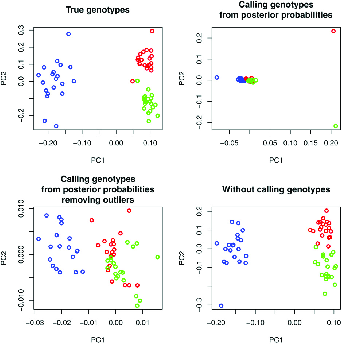
\includegraphics[width=10cm]{fumagalli-PCA.eps}
\end{center}
\caption{The ``true genotypes'' PCA is based on the actual, simulated
  genotypes (20 individuals in each population, 10,000 sites in the
  sample with 10\% variable; $F_{ST}$ between the purple population
  and either the red or the green population was 0.4 and between the
  green and red populations was 0.15; and coverage was simulated at
  $2\times$~(from~\cite{Fumagalli-etal-2013}).}\label{fig:Fumagalli-PCA}
\end{figure}

\section*{Genetic structure of human populations in Great Britain}

As we've seen several times in this course, the amount of genetic data
available on humans is vastly greater than what is available for any
other organism. As a result, it's possible to use these data to gain
unusually deep insight into the recent history of many human
populations. Today's example comes from Great Britain, courtesy of a
very large consortium~\cite{Leslie-etal-2015}

\subsection*{Data}

\begin{itemize}

\item 2039 individuals with four grandparents born within 80km of one
  another, effectively studying alleles sampled from grandparents
  (ca. 1885). 

\item 6209 samples from 10 countries in continental Europe.

\item Autosomal SNPs genotyped in both samples~(ca. 500K). 

\end{itemize}

\subsection*{Results}

Very little evidence of population structure within British sample

\begin{itemize}

\item Average pairwise $F_{ST}$: 0.0007

\item Maximum pairwise $F_{ST}$: 0.003

\end{itemize}

Individual assignment analysis of genotypes used {\tt fineSTRUCTURE},
which uses the same principle as {\tt STRUCTURE} but models the
correlations among SNPs resulting from gametic disequilibrium, rather
than treating each locus as being independently inherited. The
analysis is on {\it haplotypes\/} rather than on alleles. In addition,
it clusters populations
hierarchically~(Figure~\ref{fig:fine-structure}\index{fineSTRUCTURE}\index{human
  population genetics}

\begin{figure}
\begin{center}
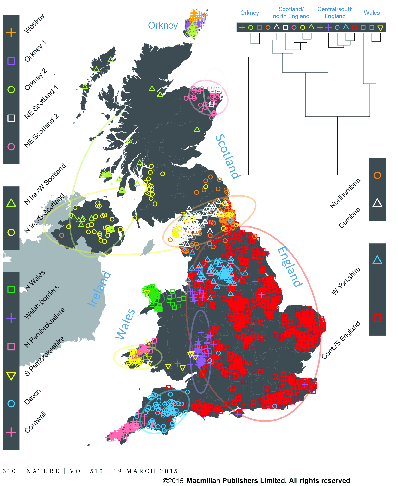
\includegraphics[height=0.9\textheight]{fine-structure-britain.eps}
\end{center}
\caption{{\tt fineSTRUCTURE} analysis of genotypes from Great Britain~(from~\cite{Leslie-etal-2015}).}\label{fig:fine-structure}
\end{figure}

Analysis of the European data identifies 52 groups. The authors used
{\tt Chromopainter} to construct each of the haplotypes detected in
their sample of 2039 individuals from the UK as a mosaic of haplotypes
derived from those found in their sample of 6209 individuals from
continental Europe. Since they know (a) the UK cluster to which each
UK individual belongs and (b) the European group from which each
individual contributing to the UK mosaic belongs they can estimate (c)
the proportion of ancestry for each UK cluster derived from each
European group. The results are shown in Figure~\ref{fig:UK-Europe}.

\begin{figure}
\begin{center}
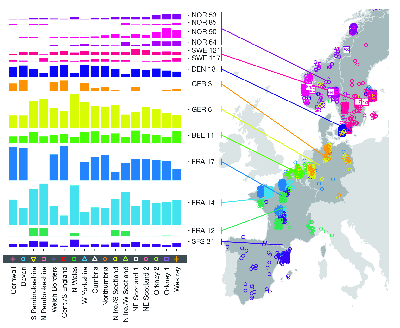
\includegraphics[width=0.9\textwidth]{UK-Europe.eps}
\end{center}
\caption{European ancestry of the 17 clusters identified in the UK~(from~\cite{Leslie-etal-2015}).}\label{fig:UK-Europe}
\end{figure}



\part{Quantitative genetics}

\documentclass[12pt]{article}
\usepackage{lecture}
\usepackage{graphics}
\usepackage{html}
\usepackage{url}
\usepackage{epstopdf}

\newcommand{\copyrightYears}{2001-2021}

\title{Introduction to quantitative genetics}

\begin{document}

\maketitle

\thispagestyle{first}

So far in this course we have dealt entirely either with the evolution
of characters that are controlled by simple Mendelian inheritance at a
single locus or with the evolution of molecular sequences. Even last
week when we were dealing with population genomic data, data from
hundreds or thousands of loci, we were treating the variation at each
locus separately and combining results across loci. I have some old
notes on gametic disequilibrium and how allele frequencies change at
two loci simultaneously, but they're in the ``Old notes, no longer
updated'' section of the book version of these
notes~(\url{https://figshare.com/articles/journal_contribution/Lecture_notes_in_population_genetics/100687}),
and we didn't discuss them.\footnote{We will spend some time talking
  about gametic disequilibrium when we talk about association mapping
  in a couple of weeks.} In every example we've considered so far
we've imagined that we could understand something about evolution by
examining the evolution of a single gene. That's the domain of
classical population genetics.

For the next few weeks we're going to be exploring a field that's
older than classical population genetics, although the approach we'll
be taking to it involves the use of population genetic
machinery.\footnote{In fact, it involves the use of the single-locus
  population genetic machinery we've been using all semester.} If you
know a little about the history of evolutionary biology, you may know
that after the rediscovery of Mendel's work in 1900 there was a heated
debate between the ``biometricians'' (e.g., Galton and Pearson) and
the ``Mendelians'' (e.g., de Vries, Correns, Bateson, and
Morgan).\index{biometricians}\index{Mendelians}

Biometricians asserted that the really important variation in
evolution didn't follow Mendelian rules. Height, weight, skin color,
and similar traits seemed to

\begin{itemize}

\item vary continuously,

\item show blending inheritance, and

\item show variable responses to the environment.

\end{itemize}

\noindent Since variation in such {\it quantitative traits\/} seemed
to be more obviously related to organismal adaptation than the
``trivial'' traits that Mendelians studied, it seemed obvious to the
biometricians that Mendelian geneticists were studying a phenomenon
that wasn't particularly interesting.\index{quantitative traits}\index{blending inheritance}

Mendelians dismissed the biometricians, at least in part, because they
seemed not to recognize the distinction between genotype and
phenotype. It seemed to at least some Mendelians that traits whose
expression was influenced by the environment were, by definition, not
inherited. Moreover, the evidence that Mendelian principles accounted
for the inheritance of many discrete traits was incontrovertible.

Woltereck's~\cite{Woltereck-1909} experiments on {\it Daphnia\/}
helped to show that traits whose expression is environmentally
influenced may also be inherited. He introduced the idea of a {\it
  norm of reaction} to describe the observation that the same genotype
may produce different phenotypes in different
environments~(Figure~\ref{fig:norm-of-reaction}). When you fertilize a
plant, for example, it will grow larger and more robust than when you
don't. The phenotype an organism expresses is, therefore, a product of
{\it both\/} its genotype and its environment.\index{norm of reaction}\index{phenotypic plasticity}

\begin{figure}
\begin{center}
\resizebox{!}{6cm}{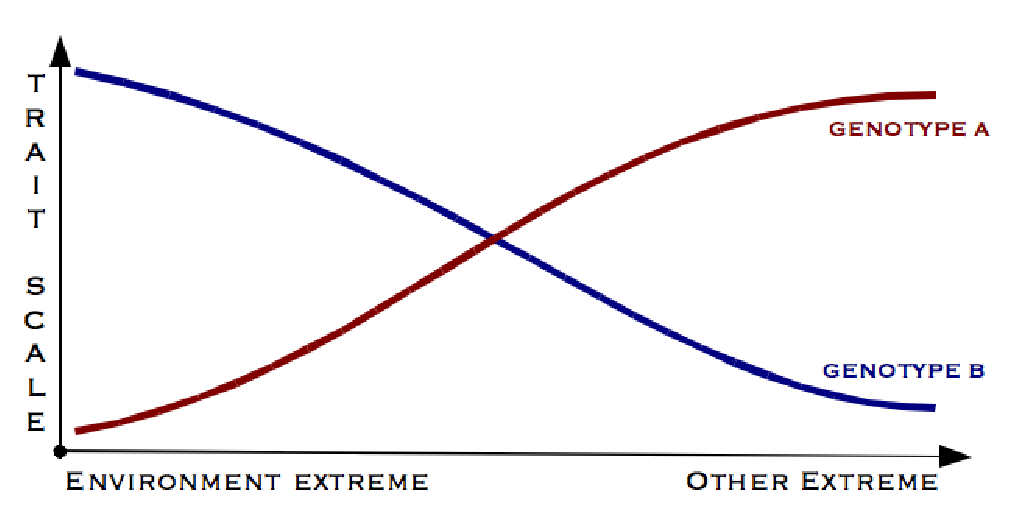
\includegraphics{Trait-scale-linear.eps}}
\end{center}
\caption{Hypothetical illustration of reaction norms for two genotypes
  across a 1-dimensional environmental gradient~(from Wikipedia,
  Public Domain,
  {\tt https://en.wikipedia.org/w/index.php?curid=3925138}, accessed 9
  April 2017).}\label{fig:norm-of-reaction}
\end{figure}

Nilsson-Ehle's~\cite{NilssonEhle-1909} experiments on inheritance of
kernel color in wheat showed how continuous variation and Mendelian
inheritance could be reconciled~(Figure~\ref{fig:nilsson-ehle}). He
demonstrated that what appeared to be continuous variation in color
from red to white with blending inheritance could be understood as the
result of three separate genes influencing kernel color that were
inherited separately from one another. It was the first example of
what's come to be known as {\it polygenic inheritance}. Fisher~\cite{Fisher-1918}, in a paper that grew out of
his undergraduate Honors thesis at Cambridge University, set forth the
mathematical theory that describes how it all works. That's the theory
of {\it quantitative genetics}, and it's what we're going to spend the
next several weeks discussing.\index{polygenic inheritance}

\begin{figure}
\begin{center}
\resizebox{!}{10cm}{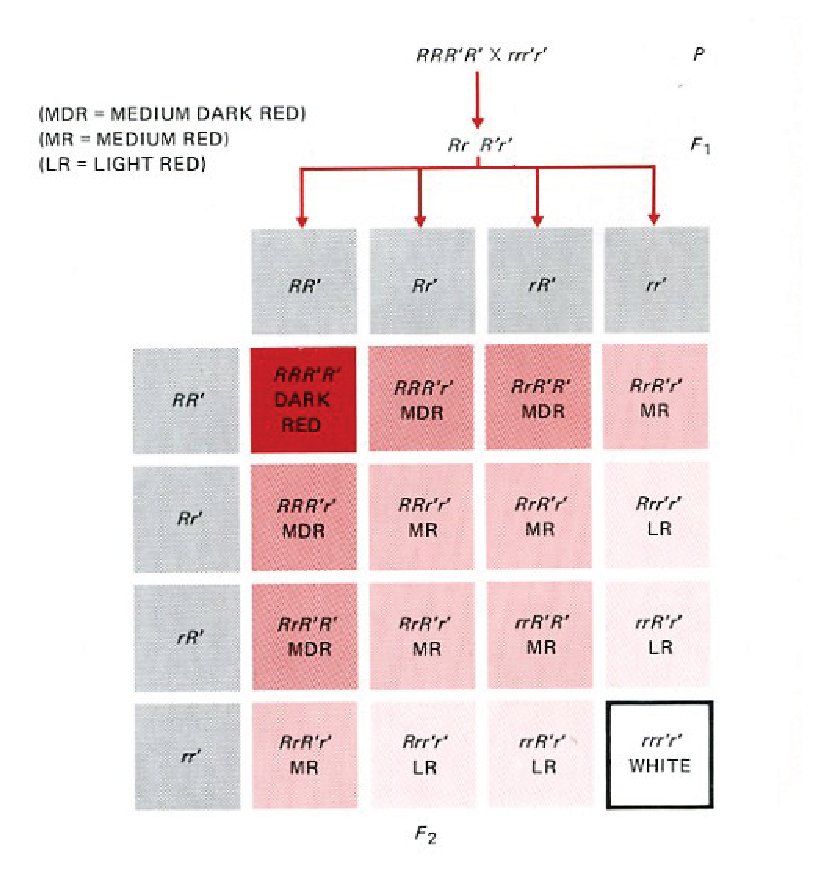
\includegraphics{Nilsson-Ehle.eps}}
\end{center}
\caption{Results from one of Nilsson-Ehle's crosses illustrating
  polygenic inhertance of kernel color in wheat~(from {\tt
    http://www.biology-pages.info/Q/QTL.html}, accessed 9 April 2017).}\label{fig:nilsson-ehle}
\end{figure}

\section*{An overview of where we're headed}

Woltereck's ideas force us to realize that when we see a phenotypic
difference between two individuals in a population there are three
possible sources for that difference:

\begin{enumerate}

\item The individuals have different genotypes.

\item The individuals developed in different environments.

\item The individuals have different genotypes {\it and\/} they
developed in different environments.

\end{enumerate}

\noindent This leads us naturally to think that phenotypic variation
consists of two separable components, namely genotypic and
environmental components.\footnote{We'll soon see that separating
  genotypic and environmental components is far from trivial. I'm also
  putting aside, for the moment, that genotypes may differ in their
  response to the environment, even though that's what I illustrated
  in discussing norms of reaction.} Putting that into an equation
\[
\Var(P) = \Var(G) + \Var(E) \quad ,
\]
where $\Var(P)$ is the {\it phenotypic variance}, $\Var(G)$ is the
{\it genetic variance}, and $\Var(E)$ is the environmental
variance.\footnote{Strictly speaking we should also include a term for
  the interaction between genotype and environment, but we'll ignore
  that for the time being. I illustrated the interaction between
  genotype and environment in discussing norms of reaction.} As
we'll see in just a moment, we can also partition the genetic variance
into components, the {\it additive genetic variance\/}, $\Var(A)$, and
the {\it dominance variance}, $\Var(D)$.\footnote{We could even
  partition it further into additive by additive, additive by
  dominance, and dominance by dominance epistatic variance, but let's
  not go there.}\index{phenotypic variance!partitioning}\index{genetic
  variance}\index{environmental variance}

There's a surprisingly subtle and important insight buried in that
very simple equation: Because the expression of a quantitative trait
is a result both of genes involved in that trait's expression and the
environment in which it is expressed, it doesn't make sense to say of
a particular individual's phenotype that genes are more important than
environment in determining it. You wouldn't have a phenotype without
both. At most what we can say is that when we look at a particular
population of organisms some fraction of the phenotypic variation they
exhibit is due to differences in the genes they carry and that some
fraction is due to differences in the environment they have
experienced.\footnote{When I put it this way, I hope it's obvious that
  I'm neglecting genotype-environment interactions, and that I'm
  oversimplifying a lot.}\index{nature vs.\ nurture} If we have two
individuals with different phenotypes, e.g., Ralph is tall and Harry
is short, we can't even say whether the difference between Ralph and
Harry is because of differences in their genes or differences in their
developmental environment.

One important implication of this insight is that much of the ``nature
vs.\ nurture'' debate concerning human intelligence or human
personality characteristics is misguided. The intelligence and
personality that you have is a product of {\it both} the genes you
happened to inherit and the environment that you happened to
experience. Any differences between you and the person next to you
probably reflect both differences in genes {\it and\/} differences in
environment. Moreover, even if the differences between you and your
neighbor are due to differences in genes, it doesn't mean that those
differences are fixed and indelible. You may be able to do something
to change them.

Take phenylketonuria, for example. It's a condition in which
individuals are homozygous for a deficiency that prevents them from
metabolizing
phenylalanine~(\url{https://medlineplus.gov/phenylketonuria.html}).
If individuals with phenylketonuria eat a normal diet, severe
intellectual disabilities can result by the time an infant is one year
old. But if they eat a diet that is very low in phenylalanine, their
development is completely normal.\index{phenylketonuria} In other
words, clear genetic differences at this locus {\it can\/} lead to
dramatic differences in cognitive ability, but {\it they don't have
  to}.

It's often useful to talk about how much of the phenotypic variance is
a result of additive genetic variance or of genetic variance.
\[
h^2_n = \frac{\Var(A)}{\Var(P)}
\]
is what's known as the {\it narrow-sense heritability}. It's the
proportion of phenotypic variance that's attributable to differences
among individuals in their additive genotype,\footnote{Don't worry
  about what I mean by {\it additive genotype}{\dash}yet. We'll get to
  it soon enough.} much as $F_{st}$ can be thought of as the
proportion of genotypic diversity that attributable to differences
among populations.\index{heritability!narrow sense} Similarly,
\[
h^2_b = \frac{\Var(G)}{\Var(P)}
\]
is the {\it broad-sense heritability}. It's the proportion of
phenotypic variance that's attributable to differences among
individuals in their genotype. It is {\it not}, repeat {\bf\it NOT}, a
measure of how important genes are in determining phenotype. Every
individuals phenotype is determined both by its genes and by its
phenotype. It measures how much of the {\it difference\/} among
individuals is attributable to differences in their genes.\footnote{As
  we'll see later it can do this only for the range of environments in
  which it was measured.}\index{heritability!broad sense} Why bother
to make the distinction between narrow- and broad-sense heritability?
Because, as we'll see, it's only the additive genetic variance that
responds to natural selection.\footnote{Or at least only the additive
  genetic variance responds to natural selection when zygotes are
  found in Hardy-Weinberg proportions.} In fact,
\[
R = h^2_nS \quad ,
\]
where $R$ is the {\it response to selection\/} and $S$ is the
{\it selective differential}.\index{response to selection}

As you'll see in the coming weeks, there's a lot of stuff hidden
behind these simple equations, including a lot of assumptions. But
quantitative genetics is very useful. Its principles have been widely
applied in plant and animal breeding for more than a century, and they
have been increasingly applied in evolutionary investigations in the
last forty years.\footnote{I used to include a joke here that I've
  decided not to include any more. It's not very funny, and some
  people might find it offensive. If for some reason you want to know
  what the joke is, you can find it in the 2017 version of these notes
  on Figshare~(\url{https://doi.org/10.6084/m9.figshare.100687.v2})}.

\section*{Partitioning the phenotypic variance}

Before we worry about how to estimate any of those variance components
I just mentioned, we first have to understand what they are. So let's
start with some
definitions~(Table~\ref{table:definitions}).\footnote{Warning! There's
  a {\it lot\/} of algebra and even a little differntial calculus
  between here and the end. It's unavoidable. You can't possibly
  understand what additive genetic variance is without it. I'll try to
  focus on principles, and I'll do my best to keep reminding us all
  why we're slogging through the math, but a lot of the math that
  follows {\it is\/} necessary. Sorry about that.}

\begin{table}
\begin{center}
\begin{tabular}{l|ccc}
\hline\hline
Genotype                 & $A_1A_1$    & $A_1A_2$ & $A_2A_2$ \\
\hline
Frequency                & $p^2$       & $2pq$    & $q^2$ \\
Genotypic value          & $x_{11}$    & $x_{12}$ & $x_{22}$ \\
Additive genotypic value & $2\alpha_1$ & $\alpha_1 + \alpha_2$
                                                  & $2\alpha_2$ \\
\hline
\end{tabular}
\end{center}
\caption{Fundamental parameter definitions for quantitative genetics
  with one locus and two alleles.}\label{table:definitions}
\end{table}\index{genotypic value}\index{additive genotypic value}\index{genotypic value!additive}

You should notice something rather strange about
Table~\ref{table:definitions} when you look at it. I motivated the
entire discussion of quantitative genetics by talking about the need
to deal with variation at many loci, and what I've presented involves
only two alleles at a single locus. I do this for two reasons:

\begin{enumerate}

\item It's not too difficult to do the algebra with multiple alleles
  at one locus instead of only two, but it gets messy, doesn't add any
  insight, and I'd rather avoid the mess.

\item Doing the algebra with multiple loci involves a {\it lot\/} of
  assumptions, which I'll mention when we get to applications, and the
  algebra is even worse than with multiple alleles.

\end{enumerate}

\noindent Fortunately, the basic principles extend with little
modification to multiple loci, so we can see all of the underlying
logic by focusing on one locus with two alleles where we have a chance
of understanding what the different variance components mean.

Two terms in Table~\ref{table:definitions} will almost certainly be
unfamiliar to you: {\it genotypic value\/} and {\it additive genotypic
  value}. Of the two, {\it genotypic value\/} is the easiest to
understand~(Figure~\ref{fig:genotypic-value}). It simply refers to the
average phenotype associated with a given
genotype.\footnote{Remember. We're now considering traits in which the
  environment influences the phenotypic expression, so the same
  genotype can produce different phenotypes, depending on the
  environment in which it develops.} The {\it additive genotypic
  value\/} refers to the average phenotype associated with a given
genotype, as would be inferred from the {\it additive effect\/} of the
alleles of which it is composed. That didn't help much, did it? That's
because I now need to tell you what we mean by the {\it additive
  effect\/} of an allele.\footnote{Hold on. Things get even more
  interesting, i.e., worse from here.}

\begin{figure}
\begin{center}
\resizebox{!}{7cm}{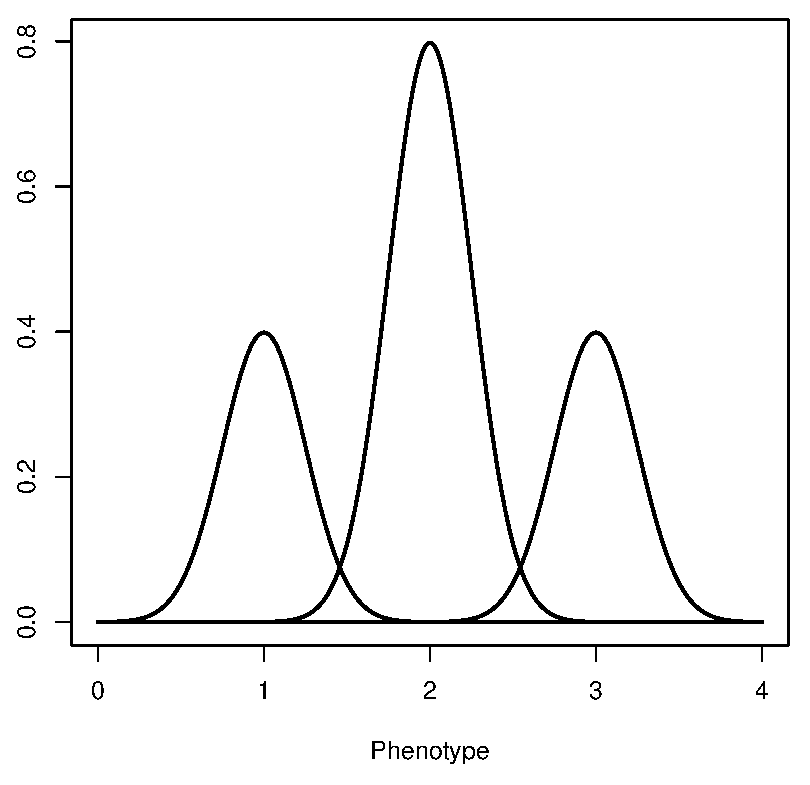
\includegraphics{genotypic-value.eps}}
\end{center}
\caption{The phenotype distribution in a population in which the three
  genotypes at a single locus with two alleles occur in Hardy-Weinberg
  proportions and the alleles occur in equal frequency. The $A_1A_1$
  genotype has a mean trait value of 1, the $A_1A_2$ genotype has a
  mean trait value of 2, and the $A_2A_2$ genotype has a mean trait
  value of 3, but each genotype can produce a range of phenotypes with
  the standard deviation of the distribution being 0.25 in each
  case.}\label{fig:genotypic-value}
\end{figure}

\subsection*{The additive effect of an allele}\index{additive effect}

In constructing Table~\ref{table:definitions} I used the quantities
$\alpha_1$ and $\alpha_2$, but I didn't tell you where they came
from. Obviously, the idea should be to pick values of $\alpha_1$ and
$\alpha_2$ that give additive genotypic values that are reasonably
close to the genotypic values. A good way to do that is to minimize
the squared deviation between the two, weighted by the frequency of
the genotypes. So our first big assumption is that genotypes are in
Hardy-Weinberg proportions.\footnote{As you should have noticed in
  Table~\ref{table:definitions}.}\index{additive effect!Hardy-Weinberg assumption}

The objective is to find values for $\alpha_1$ and $\alpha_2$ that
minimize:
\[
a = p^2[x_{11}-2\alpha_1]^2
       + 2pq[x_{12}-(\alpha_1+\alpha_2)]^2
       + q^2[x_{22}-2\alpha_2]^2 \quad .
\]
To do this we take the partial derivative of $a$ with respect to both
$\alpha_1$ and $\alpha_2$, set the resulting pair of equations equal
to zero, and solve for $\alpha_1$ and $\alpha_2$.\footnote{We won't
  bother with proving that the resulting estimates produce the minimum
  possible value of $a$. Just take my word for it. Or if you don't
  believe me and know a little calculus, take the second partials of
  $a$ and evaluate it with the values of $\alpha_1$ and $\alpha_2$
  substituted in. You'll find that the resulting matrix of partial
  derivatives, the Hessian matrix, is positive definite, meaning that
  we've found values that minimize the value of $a$. If you don't know
  what any of that means, just take my word for it that the values of
  $\alpha_1$ and $\alpha_2$ we get minimize the value of $a$.}
\begin{eqnarray*}
\frac{\partial a}{\partial{\alpha_1}} &=& p^2\{2[x_{11} - 2\alpha_1][-2]\}
                     + 2pq\{2[x_{12} - (\alpha_1+\alpha_2)][-1]\} \\
                  &=& -4p^2[x_{11} - 2\alpha_1]
                     -4pq[x_{12} - (\alpha_1+\alpha_2)] \\
\frac{\partial a}{\partial{\alpha_2}} &=& q^2\{2[x_{22} - 2\alpha_2][-2]\}
                     + 2pq\{2[x_{12} - (\alpha_1+\alpha_2)][-1]\} \\
                  &=& -4q^2[x_{22} - 2\alpha_2]
                     -4pq[x_{12} - (\alpha_1+\alpha_2)]
\end{eqnarray*}
Thus, $\frac{\partial a}{\partial{\alpha_1}} = \frac{\partial a}{\partial{\alpha_2}} = 0$ if and only if
\begin{eqnarray}
p^2(x_{11} - 2\alpha_1) + pq(x_{12} - \alpha_1 - \alpha_2) &=& 0
  \nonumber \\
q^2(x_{22} - 2\alpha_2) + pq(x_{12} - \alpha_1 - \alpha_2) &=& 0
\label{eq:zeros}
\end{eqnarray}
Adding the equations in~(\ref{eq:zeros}) we obtain (after a little bit
of rearrangement)
\begin{equation}
[p^2x_{11} + 2pqx_{12} + q^2x_{22}] -
   [p^2(2\alpha_1) + 2pq(\alpha_1 + \alpha_2) + q^2(2\alpha_2)] = 0 \quad .
\label{eq:basic}
\end{equation}

Now the first term in square brackets is just the mean phenotype in
the population, $\bar x$.  Thus, we can rewrite
equation~(\ref{eq:basic}) as:
\begin{eqnarray}
{\bar x} &=& 2p^2\alpha_1 + 2pq(\alpha_1 + \alpha_2)
                        +2q^2\alpha_2 \nonumber \\
                     &=& 2p\alpha_1(p+q) + 2q\alpha_2(p+q) \nonumber \\
                     &=& 2(p\alpha_1 + q\alpha_2) \quad . \label{eq:alpha_bar}
\end{eqnarray}
Now divide the first equation in (\ref{eq:zeros}) by $p$ and the
second by $q$.
\begin{eqnarray}
p(x_{11} - 2\alpha_1) + q(x_{12} - \alpha_1 - \alpha_2) &=& 0
\label{eq:zeros_divide_1} \\
q(x_{22} - 2\alpha_2) + p(x_{12} - \alpha_1 - \alpha_2) &=& 0 \quad
. \label{eq:zeros_divide_2}
\end{eqnarray}
Thus,
\begin{eqnarray*}
px_{11} + qx_{12} &=& 2p\alpha_1 + q\alpha_1 + q\alpha_2 \\
 &=& \alpha_1(p + q) + p\alpha_1 + q\alpha_2 \\
 &=& \alpha_1 + p\alpha_1 + q\alpha_2 \\
 &=& \alpha_1 + {\bar x}/2 \\
\alpha_1 &=& px_{11} + qx_{12} - {\bar x}/2 \quad .
\end{eqnarray*}
Similarly,
\begin{eqnarray*}
px_{12} + qx_{22} &=& 2q\alpha_2 + p\alpha_1 + p\alpha_2 \\
 &=& \alpha_2(p + q) + p\alpha_1 + q\alpha_2 \\
 &=& \alpha_2 + p\alpha_1 + q\alpha_2 \\
 &=& \alpha_2 + {\bar x}/2 \\
\alpha_2 &=& px_{12} + qx_{22} - {\bar x}/2 \quad .
\end{eqnarray*}
$\alpha_1$ is the additive effect of allele $A_1$, and $\alpha_2$ is
the additive effect of allele $A_2$. If we use these expressions, the
additive genotypic values are as close to the genotypic values as
possible, given the particular allele freequencies in the
population.\footnote{If you've been paying close attention and you
  have a good memory, the expressions for $\alpha_1$ and $\alpha_2$
  may look vaguely familiar. They look a lot like the expressions for
  marginal fitnesses we encountered when studying viability
  selection.}\index{additive effect}

\subsection*{Components of the genetic variance}\index{genetic variance!components}

Let's assume for the moment that we can actually measure the genotypic
values. Later, we'll relax that assumption and see how to use the
resemblance among relatives to estimate the genetic components of
variance. But it's easiest to see where they come from if we assume
that the genotypic value of each genotype is known. If it is then,
writing $V_g$ for $\Var(G)$
\begin{eqnarray}
V_g &=&\ p^2[x_{11} - {\bar x}]^2 + 2pq[x_{12} - {\bar x}]^2
     + q^2[x_{22} - {\bar x}]^2 \label{eq:v-g} \\
    &=&\ p^2[x_{11} - 2\alpha_1 + 2\alpha_1 - {\bar x}]^2
     + 2pq[x_{12} - (\alpha_1 + \alpha_2) + (\alpha_1 + \alpha_2)
                - {\bar x}]^2 \nonumber \\
     &&\ \ + q^2[x_{22} - 2\alpha_2 + 2\alpha_2 - {\bar x}]^2
     \nonumber \\
    &=&\ p^2[x_{11} - 2\alpha_1]^2 + 2pq[x_{12} - (\alpha_1+\alpha_2)]^2
       + q^2[x_{22} - 2\alpha_2]^2 \nonumber \\
     &&\ + p^2[2\alpha_1 - {\bar x}]^2 + 2pq[(\alpha_1 + \alpha_2) - {\bar x}]^2
       + q^2[2\alpha_2 - {\bar x}]^2 \nonumber \\
     &&\ + p^2[2(x_{11} - 2\alpha_1)(2\alpha_1 - {\bar x})]
       +2pq[2(x_{12} - \{\alpha_1+\alpha_2\})(\{\alpha_1+\alpha_2\} -
     {\bar x})] \nonumber \\
     &&\ +q^2[2(x_{22} - 2\alpha_2)(2\alpha_2 - {\bar x})] \quad .
     \label{eq:part-begin}
\end{eqnarray}
There are two terms in~(\ref{eq:part-begin}) that have a biological
(or at least a quantitative genetic) interpretation.  The term on the
first line is the average squared deviation between the genotypic
value and the additive genotypic value.  It will be zero only if the
effects of the alleles can be decomposed into strictly additive
components, i.e., only if the pheontype of the heterozygote is exactly
intermediate between the phenotype of the two homozygotes.  Thus, it
is a measure of how much variation is due to non-additivity
(dominance) of allelic effects.  In short, the {\it dominance genetic
variance}, $V_d$, is\index{dominance genetic variance}\index{genetic variance!dominance}
\begin{equation}
V_d = p^2[x_{11} - 2\alpha_1]^2 + 2pq[x_{12} - (\alpha_1+\alpha_2)]^2
          + q^2[x_{22} - 2\alpha_2]^2 \quad .\label{eq:v-d}
\end{equation}
Similarly, the term on the second line of~(\ref{eq:part-begin}) is the
average squared deviation between the additive genotypic value and the
mean genotypic value in the population.  Thus, it is a measure of how
much variation is due to differences between genotypes in their
additive genotype.  In short, the {\it additive genetic variance},
$V_a$, is\index{additive genetic variance}\index{genetic variance!dominance}
\begin{equation}
V_a = p^2[2\alpha_1 - {\bar x}]^2 + 2pq[(\alpha_1 + \alpha_2) - {\bar x}]^2
          + q^2[2\alpha_2 - {\bar x}]^2 \quad .\label{eq:v-a}
\end{equation}
What about the terms on the third and fourth lines of the last
equation in \ref{eq:part-begin}?  Well, they can be rearranged as
follows:
\begin{eqnarray*}
p^2[2(x_{11} &-& 2\alpha_1)(2\alpha_1 - {\bar x})]
 + 2pq[2(x_{12} - \{\alpha_1+\alpha_2\})(\{\alpha_1+\alpha_2\} - {\bar
 x})] \\
 &&+ q^2[2(x_{22} - 2\alpha_2)(2\alpha_2 - {\bar x})] \\
&=& 2p^2(x_{11}-2\alpha_1)(2\alpha_1 - {\bar x})
   + 4pq[x_{12}-(\alpha_1+\alpha_2)][(\alpha_1+\alpha_2)-{\bar x})] \\
 &&+ 2q^2(x_{22}-2\alpha_2)(2\alpha_2 - {\bar x}) \\
&=&\ 4p^2(x_{11}-2\alpha_1)[\alpha_1 - (p\alpha_1+q\alpha_2)] \\
 &&+ 4pq[x_{12}-(\alpha_1+\alpha_2)][(\alpha_1+\alpha_2)-2(p\alpha_1+q\alpha_2)] \\
 &&+ 4q^2(x_{22}-2\alpha_2)[\alpha_2 - (p\alpha_1+q\alpha_2)] \\
&=& 4p[\alpha_1-(p\alpha_1+q\alpha_2)]
      [p(x_{11}-2\alpha_1) + q(x_{12}-\{\alpha_1+\alpha_2\})] \\
 &&+ 4q[\alpha_2-(p\alpha_1+q\alpha_2)]
      [p(x_{11}-2\alpha_1)p + q(x_{12}-\{\alpha_1+\alpha_2\})] \\
&=& 0
\end{eqnarray*}
Where we have used the identities ${\bar x} = 2(p\alpha_1 + q\alpha_2)$ [see
equation~(\ref{eq:alpha_bar})] and
\begin{eqnarray*}
p(x_{11} - 2\alpha_1) + q(x_{12} - \alpha_1 - \alpha_2) &=& 0 \\
q(x_{22} - 2\alpha_2) + p(x_{12} - \alpha_1 - \alpha_2) &=& 0
\end{eqnarray*}
[see equations~(\ref{eq:zeros_divide_1}) and (\ref{eq:zeros_divide_2})].
In short, we have now shown that the total genotypic variance in the
population, $V_g$, can be subdivided into two components{\dash}the
additive genetic variance, $V_a$, and the dominance genetic variance,
$V_d$.  Specifically,
\[
V_g = V_a + V_d \quad ,
\]
where $V_g$ is given by the first line of (\ref{eq:v-g}), $V_a$
by (\ref{eq:v-a}), and $V_d$ by (\ref{eq:v-d}).

\subsection*{An alternative expression for $V_a$}\index{genetic variance!additive}

There's another way to write the expression for $V_a$ when there are
only two alleles at a locus. I show it here because it will come in
handy later.
\begin{eqnarray*}
V_a &=& p^2(2\alpha_1)^2 + 2pq(\alpha_1+\alpha_2)^2 + q^2(2\alpha_2)^2 -
        4(p\alpha_1+q\alpha_2)^2 \\
    &=& 4p^2\alpha_1^2 + 2pq(\alpha_1+\alpha_2)^2 + 4q^2\alpha_2^2
       - 4(p^2\alpha_1^2 +2pq\alpha_1\alpha_2 + q^2\alpha_2^2) \\
    &=& 2pq[(\alpha_1+\alpha_2)^2 - 4\alpha_1\alpha_2] \\
    &=& 2pq[(\alpha_1^2 + 2\alpha_1\alpha_2 + \alpha_2^2) - 4\alpha_1\alpha_2] \\
    &=& 2pq[\alpha_1^2 - 2\alpha_1\alpha_2 + \alpha_2^2] \\
    &=& 2pq[\alpha_1 - \alpha_2]^2 \\
    &=& 2pq\alpha^2 \\
\end{eqnarray*}

\subsection*{An example: the genetic variance with known genotypes}

We've been through a lot of algebra by now. Let's run through a couple
of numerical examples to see how it all works. For the first one,
we'll use the set of genotypic values in Table~\ref{table:additive}.

\begin{table}
\begin{center}
\begin{tabular}{l|ccc}
\hline\hline
Genotype        & $A_1A_1$ & $A_1A_2$ & $A_2A_2$ \\
Genotypic value &  100       & 50        & 0 \\
\hline
\end{tabular}
\end{center}
\caption{A set of perfectly additive genotypic values. Note that the
  genotypic value of the heterozygote is exactly halfway between the
  genotypic values of the two homozygotes.}\label{table:additive}
\end{table}

For $p = 0.4$
\begin{eqnarray*}
{\bar x} &=& (0.4)^2(100) + 2(0.4)(0.6)(50) + (0.6)^2(0) \\
                    &=& 40 \\
\\
\alpha_1 &=& (0.4)(100) + (0.6)(50) - (40)/2 \\
         &=& 50.0 \\
\alpha_2 &=& (0.4)(50) + (0.6)(0) - (40)/2 \\
         &=& 0.0 \\
\\
V_g &=& (0.4)^2(100-40)^2 + 2(0.4)(0.6)(50-40)^2 + (0.6)^2(0-40)^2 \\
    &=& 1200 \\
V_a &=& (0.4)^2[2(50.0)-20]^2 + 2(0.4)(0.6)[(50.0+0.0)-20]^2
       + (0.6)^2[2(0.0)-20]^2 \\
    &=& 1200 \\
V_d &=& (0.4)^2[2(50.0) - 100]^2 + 2(0.4)(0.6)[(50.0+0.0) - 50]^2
       + (0.6)^2[2(0.0) - 0]^2 \\
    &=& 0.00 \quad .
\end{eqnarray*}
For $p = 0.2$, ${\bar x} = 20$, $V_g = V_a = 800$, $V_d = 0.00$.  You
should verify for yourself that $\alpha_1=50$ and $\alpha_2=0$ for
$p=0.2$.  If you are ambitious, you could try to prove that
$\alpha_1=50$ and $\alpha_2=0$ for {\it any\/} allele frequency.

For the second example we'll use the set of genotypic values in
Table~\ref{table:non-additive}.

\begin{table}
\begin{center}
\begin{tabular}{l|ccc}
\hline\hline
Genotype        & $A_1A_1$ & $A_1A_2$ & $A_2A_2$ \\
Genotypic value & 100        & 80      & 0 \\
\hline
\end{tabular}
\end{center}
\caption{A set of non-additive genotypic values. Note that the
  genotypic value of the heterozygote is closer to the genotypic value
  of $A_1A_1$ than it is to the genotypic value of $A_2A_2$.}\label{table:non-additive}
\end{table}

For $p = 0.4$
\begin{eqnarray*}
{\bar x} &=& (0.4)^2(100) + 2(0.4)(0.6)(80) + (0.6)^2(0) \\
                    &=& 54.4 \\
\\
\alpha_1 &=& (0.4)(100) + (0.6)(80) - (54.4)/2 \\
         &=& 60.8 \\
\alpha_2 &=& (0.4)(80) + (0.6)(0) - (54.4)/2 \\
         &=& 4.8 \\
\\
V_g &=& (0.4)^2(100-54.4)^2 + 2(0.4)(0.6)(80-54.4)^2 + (0.6)^2(0-54.4)^2 \\
    &=& 1712.64 \\
V_a &=& (0.4)^2[2(60.8)-54.4]^2 + 2(0.4)(0.6)[(60.8+4.8)-54.4]^2 \\
       &&+ (0.6)^2[2(9.6)-54.4]^2 \\
    &=& 1505.28 \\
V_d &=& (0.4)^2[2(60.8)-100]^2 + 2(0.4)(0.6)[(60.8+4.8) - 80]^2 \\
       &&+ (0.6)^2[2(9.6)-0]^2 \\
    &=& 207.36 \quad .
\end{eqnarray*}

To test your understanding, it would probably be useful to calculate
${\bar x}$, $\alpha_1$, $\alpha_2$, $V_g$, $V_a$, and $V_d$ for one or
two other allele frequencies, say $p=0.2$ and $p=0.8$.\footnote{The
  easy way to do this, of course, would be to have the R Shiny app do
  the calculation for you. I recommend that you try it on your own and
  compare your answers with what R Shiny reports.} Is it still true
that $\alpha_1$ and $\alpha_2$ are independent of allele frequencies?
If you are {\it really\/} ambitious you could try to prove that
$\alpha_1$ and $\alpha_2$ are independent of allele frequencies if and
only if $x_{12} = (x_{11}+x_{12})/2$, i.e., when heterozygotes are
exactly~intermediate.

\bibliography{popgen}
\bibliographystyle{plain}

\ccLicense

\end{document}

\documentclass[12pt]{article}
\usepackage{lecture}
\usepackage{graphics}
\usepackage{html}
\usepackage{url}

\newcommand{\copyrightYears}{2001-2021}

\title{Resemblance among relatives}

\begin{document}

\maketitle

\thispagestyle{first}

\section*{Introduction}

Just as individuals may differ from one another in phenotype because
they have different genotypes, because they developed in different
environments, or both, relatives may resemble one another more than
they resemble other members of the population because they have
similar genotypes, because they developed in similar environments, or
both. In an experimental situation, we typically try to randomize
individuals across environments. If we are successful, then any
tendency for relatives to resemble one another more than non-relatives
must be due to similarities in their genotypes.\index{resemblance between relatives}

Using this insight, we can develop a statistical technique that allows
us to determine how much of the variance among individuals in
phenotype is a result of genetic variance and how much is due to
environmental variance. {\it Remember}, we can only ask about how much
of the variability is due to genetic differences, and we can only do
so {\it in a particular environment\/} and {\it with a particular set
of genotypes}, and we can only do it when we {\it randomize genotypes
  across environments}.

\section*{An outline of the approach}

The basic approach to the analysis is either to use a linear
regression of offspring phenotype on parental phenotype, which as
we'll see estimates $h^2_n$, or to use a nested analysis of
variance. One of the most complete designs is a full-sib, half-sib
design in which each male sires offspring from several dams but each
dam mates with only one sire.\index{parent-offspring regression}\index{full-sib analysis}

The offspring of a single dam are full-sibs (they are nested within
dams). Differences among the offspring of dams indicates that there
are differences in maternal ``genotype'' in the trait being
measured.\footnote{Assuming that we've randomized siblings across
  environments. If we haven't, siblings may resemble one another
  because of similarities in the environment they experienced, too.}

The offspring of different dams mated to a single sire are
half-sibs. Differences among the offspring of sires indicates that
there are differences in paternal ``genotype'' in the trait being
measured.\footnote{You'll see the reason for the quotes around
  genotype in this paragraph and the last a little later. It's a
  little more complex than what I've suggested.}

As we'll see, this design has the advantage that it allows both
additive and dominance components of the genetic variance to be
estimated. It has the additional advantage that we don't have to
assume that the distribution of environments in the offspring
generation is the same as it was in the parental generation. To use
the regression approach to estimate heritability, we have to assume
that the distribution of environmental effects is the same in parental
and offspring generations.\index{full-sib analysis!advantages}

\section*{The gory details}

OK, so I've given you the basic idea. Where does it come from, and how
does it work? Funny you should ask. The whole approach is based on
calculations of the degree to which different relatives resemble one
another. For these purposes we're going to continue our focus on
phenotypes influenced by one locus with two alleles, and we'll do the
calculations in detail only for half sib families. We start with
something that may look vaguely familiar.\footnote{Remember our
  mother-offspring combinations with {\it Zoarces viviparus\/}?} Take
a look at Table~\ref{table:half-sib}.\index{mother-offspring
  pairs}\index{half-sib analysis}

\begin{table}
\begin{center}
\begin{tabular}{c|c|ccc}
\hline\hline
Maternal &           & \multicolumn{3}{c}{Offspring genotype} \\
genotype & Frequency & $A_1A_1$      & $A_1A_2$      & $A_2A_2$ \\
\hline
$A_1A_1$ & $p^2$     & $p$           & q             & 0 \\
$A_1A_2$ & $2pq$     & $\frac{p}{2}$ & $\frac{1}{2}$ & $\frac{q}{2}$ \\
$A_2A_2$ & $q^2$     & 0             & p             & q \\
\hline
\end{tabular}
\end{center}
\caption{Half-sib family structure in a population with genotypes in
  Hardy-Weinberg proportions.}\label{table:half-sib}
\end{table}

Note that the probabilities in Table~\ref{table:half-sib} are
appropriate {\it only\/} if the progeny are from half-sib families.
If the progeny are from full-sib families, we must specify the
frequency of each of the nine possible matings (keeping track of the
genotype of both mother and father) and the offspring that each will
produce.\footnote{To check your understanding of all of this, you
  might want to try to produce the appropriate table.}

\subsection*{Covariance of two random variables}\index{covariance}

Let $p_{xy}$ be the probability that random variable $X$ takes the
value $x$ and random variable $Y$ takes the value $y$.  Then the
covariance between $X$ and $Y$ is:
\[
\Cov(X,Y) = \sum p_{xy}(x - \mu_x)(y - \mu_y) \quad ,
\]
where $\mu_x$ is the mean of $X$ and $\mu_y$ is the mean of $Y$. The
covariance between two random variables is a measure of how much they
vary together{\dash}covary. If the covariance is large and positive,
they tend to vary in the same way. Positive deviations from the mean
in one are associated with positive deviations from the mean in the
other, and negative deviations are similarly associated. If the
covariance is large and negative, they tend to vary in opposite
ways. Positive deviations from the mean in one variable are associated
with {\it negative\/} deviations in the other, and vice versa. If the
covariance is small, it means there isn't a strong tendency for
deviations from the mean in one variable to be associated with
deviations in the other.

\subsection*{Covariance between half-siblings}\index{covariance!half-siblings}

Here's how we can calculate the covariance between half-siblings:
First, imagine selecting huge number of half-sibs pairs at random.
The phenotype of the first half-sib in the pair is a random variable
(call it $S_1$), as is the phenotype of the second (call it $S_2$).
The mean of $S_1$ is just the mean phenotype in {\it all\/} the
progeny taken together, $\bar x$.  Similarly, the mean of $S_2$ is
just $\bar x$.\footnote{The reasoning here gets a little tricky, since
  the mean of different half-sib families may be different. Think
  about it this way. We picked this particular half-sib family at
  random from among all half-sib families in the population. It takes
  a bit of algebra to show it, but the mean phenotype of a randomly
  chosen half-sib family is $\bar x$, meaning that $\bar x$ is the
  mean phenotype for both $S_1$ and $S_2$. They're part of the same
  family, so they share the same family mean.}  Now with one locus,
two alleles we have three possible phenotypes: $x_{11}$ (corresponding
to the genotype $A_1A_1$), $x_{12}$ (corresponding to the genotype
$A_1A_2$), and $x_{22}$ (corresponding to the genotype $A_2A_2$).  So
all we need to do to calculate the covariance between half-sibs is to
write down all possible pairs of phenotypes and the frequency with
which they will occur in our sample of randomly chosen half-sibs based
on the frequencies in Table~\ref{table:half-sib} above and the
frequency of maternal genotypes.  It's actually a bit easier to keep
track of it all if we write down the frequency of each maternal
genotype and the frequency with which each possible phenotypic
combination will occur in her progeny.
\begin{eqnarray*}
\Cov(S_1,S_2) &=& p^2[p^2(x_{11} - {\bar x})^2 + 2pq(x_{11} - {\bar x})
                                                (x_{12} - {\bar x})
                                           + q^2(x_{12} - {\bar x})^2] \\
             &&+ 2pq[{1 \over 4}p^2(x_{11} - {\bar x})^2
                  + {1 \over 2}p(x_{11} - {\bar x})(x_{12} - {\bar x})
                  + {1 \over 2}pq(x_{11} - {\bar x})(x_{22} - {\bar x}) \\
             &&\ \ + {1 \over 4}(x_{12} - {\bar x})^2
                  + {1 \over 2}q(x_{12} - {\bar x})(x_{22} - {\bar x})
                  + {1 \over 4}q^2(x_{22} - {\bar x})^2] \\
             &&+ q^2[p^2(x_{12} - {\bar x})^2 + 2pq(x_{12} - {\bar
                x})(x_{22} - {\bar x})
                                                 + q^2(x_{22} - {\bar
                                                x})^2] \\
   &=&\ p^2[p(x_{11} - {\bar x}) + q(x_{12} - {\bar x})]^2 \\
   &&+ 2pq[{1 \over 2}p(x_{11} - {\bar x}) +
         {1 \over 2}q(x_{12} - {\bar x}) +
         {1 \over 2}p(x_{12} - {\bar x}) +
         {1 \over 2}q(x_{22} - {\bar x})]^2 \\
   &&+ q^2[p(x_{12} - {\bar x}) + q(x_{22} - {\bar x})]^2 \\
   &=&\ p^2[px_{11} + qx_{12} - {\bar x}]^2 \\
   &&+ 2pq\left[{1 \over 2}(px_{11} + qx_{12} - {\bar x}) +
         {1 \over 2}(px_{12} + qx_{22} - {\bar x})\right]^2 \\
   &&+ q^2[px_{12} + qx_{22} - {\bar x}]^2 \\
   &=&\ p^2\left[\alpha_1 - {{\bar x} \over 2}\right]^2
   + 2pq\left[{1 \over 2}(\alpha_1 - {{\bar x} \over 2}) +
         {1 \over 2}(\alpha_2 - {{\bar x} \over 2})\right]^2
   + q^2\left[\alpha_2 - {{\bar x} \over 2}\right]^2 \\
   &=&\ p^2\left[{1 \over 2}(2\alpha_1 - {\bar x})\right]^2
   + 2pq\left[{1 \over 2}(\alpha_1 + \alpha_2 - {\bar x})\right]^2
        + q^2\left[{1 \over 2}(2\alpha_2 - {\bar x})\right]^2 \\
   &=& \left({1 \over 4}\right)
      \left[p^2(2\alpha_1 - {\bar x})^2
        + 2pq[(\alpha_1+\alpha_2 - {\bar x})]^2
        + q^2(2\alpha_2 - {\bar x})^2\right] \\
   &=& \left({1 \over 4}\right)V_a
\end{eqnarray*}

\subsection*{A numerical example}

Now we'll return to an example we saw
earlier~(Table~\ref{table:example}). This set of genotypes and
phenotypes may look familiar. It is the same one we encountered
earlier when we calculated additive and dominance components of
variance. Let's assume that $p = 0.4$. We know from our earlier
calculations that
\begin{eqnarray*}
\bar x &=& 54.4 \\
V_a &=& 1505.28 \\
V_d &=& 207.36 \quad .
\end{eqnarray*}
We can also calculate the numerical version of
Table~\ref{table:half-sib}, which you'll find in
Table~\ref{table:example-hs}.

\begin{table}
\begin{center}
\begin{tabular}{l|ccc}
\hline\hline
Genotype  & $A_1A_1$ & $A_1A_2$ & $A_2A_2$ \\
Phenotype & 100        & 80      & 0 \\
\hline
\end{tabular}
\end{center}
\caption{An example of a non-additive relationship between genotypes
  and phenotypes.}\label{table:example}
\end{table}

\begin{table}
\begin{center}
\begin{tabular}{c|c|ccc}
\hline\hline
Maternal &           & \multicolumn{3}{c}{Offspring genotype} \\
genotype & Frequency & $A_1A_1$ & $A_1A_2$ & $A_2A_2$ \\
\hline
$A_1A_1$ & 0.16      & 0.4      & 0.6      & 0.0 \\
$A_1A_2$ & 0.48      & 0.2      & 0.5      & 0.3 \\
$A_2A_2$ & 0.36      & 0.0      & 0.4      & 0.6 \\
\hline
\end{tabular}
\end{center}
\caption{Mother-offspring combinations (half-sib) when the frequency
  of $A_1$ is 0.4.}\label{table:example-hs}
\end{table}

So now we can follow the same approach we did before and calculate the
numerical value of the covariance between half-sibs in this example:
\begin{eqnarray*}
\Cov(S_1,S_2) &=&\ [(0.4)^2(0.16) + (0.2)^2(0.48)](100 - 54.4)^2 \\
          && + [(0.6)^2(0.16) + (0.5)^2(0.48) + (0.4)^2(0.36)] (80 - 54.4)^2 \\
          && + [(0.3)^2(0.48) + (0.6)^2(0.36)](0 - 54.4)^2 \\
          && + 2[(0.4)(0.6)(0.16) + (0.2)(0.5)(0.48)](100 - 54.4)(80 - 54.4) \\
          && + 2(0.2)(0.3)(0.48)(100 - 54.4)(0 - 54.4) \\
          && + 2[(0.5)(0.3)(0.48) + (0.4)(0.6)(0.36)](80 - 54.4)(0 - 54.4) \\
         &=&\ 376.32 \\
         &=&\ \left({1 \over 4}\right)1505.28 \quad .
\end{eqnarray*}

\subsection*{Covariances among relatives}\index{covariance!relatives}

Well, if we can do this sort of calculation for half-sibs, you can
probably guess that it's also possible to do it for other relatives. I
won't go through all of the calculations, but the results for common
forms of relationship are summarized in Table~\ref{table:relatives}

\begin{table}
\begin{center}
\begin{tabular}{ll}
\hline\hline
MZ twins ($\Cov_{MZ}$) & $V_a + V_d$ \\
Parent-offspring ($\Cov_{PO}$)$^1$ & $\left(\frac{1}{2}\right)V_a$ \\
Full sibs ($\Cov_{FS}$) & $\left(\frac{1}{2}\right)V_a +
\left(\frac{1}{4}\right)V_d$ \\
Half sibs ($\Cov_{HS}$) & $\left(\frac{1}{4}\right)V_a$ \\
\hline
\multicolumn{2}{l}{$^1$One parent or mid-parent.}
\end{tabular}
\end{center}
\caption{Genetic covariances among relatives.}\label{table:relatives}
\end{table}

\section*{Estimating heritability}\index{heritability}

Galton introduced the term {\it regression\/} to describe the
inheritance of height in humans. He noted that there is a tendency for
adult offspring of tall parents to be tall and of short parents to be
short, but he also noted that offspring tended to be less extreme than
the parents.\footnote{It's worth noting that Galton is often
  ``credited'' with establishing the field of eugenics. He was a
  proponent of encouraging the ``best'' people to marry one another to
  ``improve'' the human race. In 2020, University College London
  renamed two lecture theaters and a building that bore the names of
  Francis Galton and Karl Pearson~(\url{https://www.theguardian.com/education/2020/jun/19/ucl-renames-three-facilities-that-honoured-prominent-eugenicists}).}
He described this as a ``regression to mediocrity,'' and statisticians
adopted the term to describe a standard technique for describing the
functional relationship between two~variables.

\subsection*{Regression analysis}\index{parent-offspring regression}

Measure the parents.  Regress the offspring phenotype on: (1) the
phenotype of one parent or (2) the mean of the parental
phenotypes.  In either case, the covariance between the parental
phenotype and the offspring genotype is $\left({1 \over 2}\right)V_a$.
Now the regression coefficient between one parent and offspring, $b_{P
\rightarrow O}$, is
\begin{eqnarray*}
b_{P \rightarrow O}
&=& \frac{\Cov_{PO}}{\Var(P)} \\
&=& {\left({1 \over 2}\right)V_a \over V_p} \\
&=& \left({1 \over 2}\right)h^2_N \quad .
\end{eqnarray*}
In short, the slope of the regression line is equal to one-half the
narrow sense heritability.  In the regression of offspring on
mid-parent value,
\begin{eqnarray*}
\Var(MP) &=& \Var\left(\frac{M+F}{2}\right) \\
                  &=& \frac{1}{4} \Var(M+F) \\
                  &=& \frac{1}{4} \left(Var(M) + Var(F)\right) \\
                  &=& \frac{1}{4} \left(2V_p\right) \\
                  &=& \frac{1}{2} V_p \quad .
\end{eqnarray*}
Thus, $b_{MP \rightarrow O} = \frac{1}{2}V_a/\frac{1}{2}V_p = h^2_N$.
In short, the slope of the regression line is equal to the narrow
sense heritability.\index{heritability}

\subsection*{Sib analysis}\index{full-sib analysis}

Mate a number of males (sires) with a number of females (dams).  Each
sire is mated to more than one dam, but each dam mates only with one
sire.  Do an analysis of variance on the phenotype in the progeny,
treating sire and dam as main effects.  The result is shown in
Table~\ref{table:full-sib}.

\begin{table}
\begin{center}
\begin{tabular}{l|ccc}
\hline\hline
        &      &             & Composition of \\
Source  & d.f. & Mean square & mean square \\
\hline
Among sires             & $s-1$     & $MS_S$
                        & $\sigma^2_W + k\sigma^2_D + dk\sigma^2_s$ \\
Among dams              & $s(d-1)$  & $MS_D$
                        & $\sigma^2_W + k\sigma^2_D$ \\
\hskip 1em (within sires) \\
Within progenies        & $sd(k-1)$ & $MS_W$
                        & $\sigma^2_W$\\
\hline
\multicolumn{4}{l}{$s = \hbox{number of sires}$} \\
\multicolumn{4}{l}{$d = \hbox{number of dams per sire}$} \\
\multicolumn{4}{l}{$k = \hbox{number of offspring per dam}$}
\end{tabular}
\end{center}
\caption{Analysis of variance table for a full-sib analysis of
  quantitative genetic variation.}\label{table:full-sib}
\end{table}

Now we need some way to relate the variance components ($\sigma^2_W$,
$\sigma^2_D$, and $\sigma^2_S$) to $V_a$, $V_d$, and
$V_e$.\footnote{$\sigma^2_W$, $\sigma^2_D$, and $\sigma^2_S$ are often
  referred to as the {\it observational\/} components of variance,
  because they are estimated from observations we make on phenotypic
  variation. $V_a$, $V_d$, and $V_e$ are often referred to as the {\it
    causal\/} components of variance, because they represent the
  genetic and environmental influences on trait
  expression.}\index{components of variance!observational}\index{components of variance!causal} How do we
do that?  Well,
\[
V_p = \sigma^2_T = \sigma^2_S + \sigma^2_D + \sigma^2_W \quad .
\]
$\sigma^2_S$ estimates the variance among the means of the half-sib
families fathered by each of the different sires or, equivalently, the
covariance among half-sibs.\footnote{To see why consider this is so,
  consider the following: The mean genotypic value of half-sib
  families with an $A_1A_1$ mother is $px_{11} + qx_{12}$; with an
  $A_1A_2$ mother, $px_{11}/2 + qx_{12}/2 + px_{12}/2 + qx_{22}/2$;
  with an $A_2A_2$ mother, $px_{12} + qx_{22}$.  The equation for the
  variance among these means is identical to the equation for the
  covariance among half-sibs.}
\begin{eqnarray*}
\sigma^2_S &=& \Cov_{HS} \\
           &=& \left(\frac{1}{4}\right)V_a \quad .
\end{eqnarray*}
Now consider the within progeny component of the variance,
$\sigma^2_W$.  In general, it can be shown that {\it any\/} among
group variance component is equal to the covariance among the members
within the groups.\footnote{With $x_{ij} = a_i + \epsilon_{ij}$, where
  $a_i$ is the mean group effect and $\epsilon_{ij}$ is random effect
  on individual $j$ in group $i$ (with mean 0), $Cov(x_{ij},x_{ik}) =
  E(a_i + \epsilon_{ij} - \mu)(a_i + \epsilon_{ik} - \mu) = E((a_i
  -\mu^2) + a_i(\epsilon_{ij} + \epsilon_{ik}) +
  \epsilon_{ij}\epsilon_{ik}) = Var(A)$.}  Thus, a within group
component of the variance is equal to the total variance minus the
covariance within groups.  In this case,
\begin{eqnarray*}
\sigma^2_W &=& V_p - \Cov_{FS} \\
 &=& V_a + V_d + V_e - \left[\left(\frac{1}{2}\right)V_a +
                            \left(\frac{1}{4}\right)V_d
                      \right] \\
 &=& \left(\frac{1}{2}\right)V_a
    + \left({3 \over 4}\right)V_d
    + V_e \quad .
\end{eqnarray*}
There remains only $\sigma^2_D$.  Now $\sigma^2_W = V_p - Cov_{FS}$,
$\sigma^2_S = Cov_{HS}$, and $\sigma^2_T = V_p$.  Thus,
\begin{eqnarray*}
\sigma^2_D &=& \sigma^2_T - \sigma^2_S - \sigma^2_W \\
           &=& V_p - \Cov_{HS} - (V_p - \Cov_{FS}) \\
           &=& \Cov_{FS} - \Cov_{HS} \\
           &=& \left[
              \left(\frac{1}{2}\right)V_a + \left(\frac{1}{4}\right)V_d
              \right]
              - \left(\frac{1}{4}\right)V_a \\
           &=& \left(\frac{1}{4}\right)V_a +
           \left(\frac{1}{4}\right)V_d \quad .
\end{eqnarray*}
So if we rearrange these equations, we can express the genetic
components of the phenotypic variance, the {\it causal\/} components
of variance, as simple functions of the {\it observational} components
of variance:\index{components of variance!observational}\index{components of variance!causal}
\begin{eqnarray*}
V_a &=& 4\sigma^2_S \\
V_d &=& 4(\sigma^2_D - \sigma^2_S) \\
V_e &=& \sigma^2_W - 3\sigma^2_D + \sigma^2_S \quad .
\end{eqnarray*}
Furthermore, the narrow-sense heritability is given by
\[
h^2_N = \frac{4\sigma^2_s}{\sigma^2_S + \sigma^2_D + \sigma^2_W} \quad .
\]\index{heritability}

\subsection*{An example: body weight in female mice}\index{full-sib analysis!example}

The analysis involves 719 offspring from 74 sires and 192 dams, each
with one litter.  The offspring were spread over 4 generations, and
the analysis is performed as a nested ANOVA with the genetic analysis
nested {\it within\/} generations.  An additional complication is that
the design was unbalanced, i.e., unequal numbers of progeny were
measured in each sibship.  As a result the degrees of freedom don't
work out to be quite as simple as what I showed you.\footnote{What did
you expect from real data? This example is extracted from Falconer and
Mackay, pp.\ 169--170. See the book for details.} The results are
summarized in Table~\ref{table:mice}.

\begin{table}
\begin{center}
\begin{tabular}{l|ccc}
\hline\hline
        &      &             & Composition of \\
Source  & d.f. & Mean square & mean square \\
\hline
Among sires             & 70 & 17.10
                        & $\sigma^2_W + k'\sigma^2_D + dk'\sigma^2_s$ \\
Among dams              & 118 & 10.79
                        & $\sigma^2_W + k\sigma^2_D$ \\
\hskip 1em (within sires) \\
Within progenies        & 527 & 2.19
                        & $\sigma^2_W$ \\
\hline
\multicolumn{4}{l}{$d = 2.33$} \\
\multicolumn{4}{l}{$k = 3.48$} \\
\multicolumn{4}{l}{$k' = 4.16$} \\
\end{tabular}
\end{center}
\caption{Quantitative genetic analysis of the inheritance of body
  weight in female mice (from Falconer and Mackay,
  pp. 169--170.)}\label{table:mice}
\end{table}

Using the expressions for the composition of the mean square we
obtain
\begin{eqnarray*}
\sigma^2_W &=& MS_W \\
           &=& 2.19 \\
\sigma^2_D &=& \left({1 \over k}\right)(MS_D - \sigma^2_W) \\
           &=& 2.47 \\
\sigma^2_S &=& \left({1 \over dk'}\right)(MS_S - \sigma^2_W
                    - k'\sigma^2_D) \\
           &=& 0.48 \quad .
\end{eqnarray*}
Thus,
\begin{eqnarray*}
V_p &=& 5.14 \\
V_a &=& 1.92 \\
V_d + V_e &=& 3.22 \\
V_d &=& (0.00\hbox{---}1.64) \\
V_e &=& (1.58\hbox{---}3.22) \\
\end{eqnarray*}

Why didn't I give a definite number for $V_d$ after my big spiel above
about how we can estimate it from a full-sib crossing design?  Two
reasons.  First, if you plug the estimates for $\sigma^2_D$ and
$\sigma^2_S$ into the formula above for $V_d$ you get $V_d = 7.96, V_e
= -4.74$, which is clearly impossible since $V_d$ has to be less than
$V_p$ and $V_e$ has to be greater than zero. It's a variance.  Second,
the experimental design confounds two sources of resemblance among
full siblings: (1) genetic covariance and (2) environmental
covariance.  The full-sib families were all raised by the same mother
in the same pen. Hence, we don't know to what extent their resemblance
is due to a common natal environment.\footnote{Notice that this
  doesn't affect our analysis of half-sib families, i.e., the progeny
  of different sires, since each father was bred with several females}
If we assume $V_d = 0$, we can estimate the amount of variance
accounted for by exposure to a common natal environment, $V_{Ec} =
1.99$, and by environmental variation within sibships, $V_{Ew} =
1.23$.\footnote{See Falconer for details.}  Similarly, if we assume
$V_{Ew} = 0$, then $V_d = 1.64$ and $V_{Ec} = 1.58$.  In any case, we
can estimate the narrow sense heritability as
\begin{eqnarray*}
h^2_N &=& \left({1.92 \over 5.14}\right) \\
      &=& 0.37 \quad .
\end{eqnarray*}

\ccLicense

\end{document}

\input{quant-evolution}
\documentclass[12pt]{article}
\usepackage{lecture}
\usepackage{graphicx}
\usepackage{epstopdf}
\usepackage{html}
\usepackage{url}

\newcommand{\copyrightYears}{2010-2021}

\title{Association mapping: a (very) brief overview}

\begin{document}

\maketitle

\thispagestyle{first}

\section*{Introduction}

One approach to understanding more about the genetics of quantitative
traits takes advantage of the increasing number of genetic markers
available as a result of recent advances in molecular
genetics. Suppose you have two inbred lines that differ in a trait
that interests you, say body weight or leaf width. Call one of them
the ``high'' line and the other the ``low''
line.\footnote{Corresponding to whether the body weight or leaf width
  is large or small.} Further suppose that you have a whole bunch of
molecular markers that differ between the two lines, and designate the
genotype in the ``high'' line $A_1A_1$ and the genotype in the low
line $A_2A_2$.\footnote{Since these are inbred lines, I can assume
  that they are homozygous at the marker loci I've chosen.} One last
supposition: Suppose that at loci influencing the phenotype you're
studying the genotype in the ``high'' line is $Q_1Q_1$ and the
genotype in the ``low'' line is $Q_2Q_2$. Each of these loci is what
we call a {\it quantitative trait locus\/} or QTL.\index{quantitative trait locus}\index{QTL} Now do the following experiment:

\begin{itemize}

\item Cross the ``high'' line and the ``low'' line to construct an
  $F_1$.

\item Intercross individuals in the $F_1$ generation to form an
  $F_2$.\footnote{Note: You could also backcross to either or both of
    the parental inbred lines. Producing an $F_2$, however, allows you
    to estimate both the additive and dominance effects associated
    with each QTL.}

\item ``Walk'' through the genome\footnote{I forgot to mention another
    supposition. I am supposing that you either have already
    constructed a genetic map using your markers, or that you will
    construct a genetic map using segregation in the $F_2$ before you
    start looking for QTL loci.} calculating a likelihood score for a
  QTL at a particular map position, using what we know about the
  mathematics of recombination rates and Mendelian genetics. In
  calculating the likelihood score we maximize the likelihood of the
  data assuming that there is a QTL at this position and estimating
  the corresponding additive and dominance effects of the allele. We
  then identify QTLs as those loci where there are ``significant''
  peaks in the map of likelihood scores.

\end{itemize}
The result is a genetic map showing where QTLs are in the genome and
indicating the magnitude of their additive and dominance effects.

QTL mapping is wonderful{\dash}provided that you're working with an
organism where it's possible to design a breeding program and where
the information derived from that breeding program is relevant to
variation in natural populations. Think about it. If we do a QTL
analysis based on segregation in an $F_2$ population derived from two
inbred lines, all we really know is which loci are associated with
phenotypic differences {\it between those two lines}. Typically what
we really want to know, if we're evolutionary biologists, is which
loci are associated with phenotypic differences {\it between
  individuals in the population we're studying}. That's where
association mapping comes in. We look for statistical associations
between phenotypes and genotypes across a whole population. We expect
there to be such associations, if we have a dense enough map, because
some of our marker loci will be closely linked to loci responsible for
phenotypic variation.\index{QTL mapping}

\section*{Association mapping}

So how does association mapping work? There are two broad approaches,
one that is used in genome-wide association studies (GWAS) that is
analogous to QTL mapping and one that looks for differences between
``cases,'' those that exhibit a particular phenotype of
interest~(e.g., a disease state in humans), and ``controls,'' those
that don't exhibit the phenotype of interest. Let's talk about GWAS
first.\index{Genome-wide association study}\index{case-control study}

\subsection*{Genome-wide association study}

\subsubsection*{Principles}

Imagine that we have a well-mixed population segregating both for a
lot of molecular markers spread throughout the genome and for loci
influencing a trait we're interested in, like body weight or leaf
width. Let's call our measurement of that trait $z_i$ in the $i$th
individual. Let $x_{ij}$ be the genotype of individual $i$ at the
$j$th locus.\footnote{To keep things simple I'm assuming that we're
  dealing with biallelic loci, e.g., SNPs, and we can then order the
  genotypes as 0, 1, 2 depending on how many copies of the most
  frequent allele they carry. So $x_{ij}$ is the number of copies of
  $A_1$ individual $i$ carries at locus $j$.} Then to do association
mapping, we simply fit the following regression model:
\[
y_i = x_{ij}\beta_j + \epsilon_{ij} \quad ,
\]
where $\epsilon_{ij}$ is the residual error in our regression estimate
and $\beta_j$ is our estimate of the effect of substituting one allele
for another at locus $j$, i.e., the additive effect of an allele at
locus $j$.\footnote{We can generalize the regression to allow us to
  estimate dominance effects too, but doing so only complicates the
  algebra without providing any additional insight.} If $\beta_j$ is
significantly different from 0, we have evidence that there is a locus
linked to this marker that influences the phenotype we're interested
in, and we have an estimate of the additive effect of the alleles at
that locus.

Notice that I claimed we have evidence that the locus is
linked. That's a bit of sleight of hand. I've glossed over something
very important. What we have direct evidence for is only that the
locus is {\it associated} with the phenotype differences. As we'll see
in just a bit, the observed association {\it might\/} reflect physical
linkage between the marker locus and a locus influencing the phenotype
or it could reflect a statistical association that arises for other
reasons, including population structure. So in practice the regression
model we fit is a more complicated than the one I just described. The
simplest case is when individuals fall into obvious groups, e.g.,
samples from different populations. Then $y_i^{(k)}$ is the trait
value for individual $i$. The superscript $(k)$ indicates that this
individual belongs to group $k$.
\[
y_i^{(k)} = x_{ij}\beta_j + \phi^{(k)} + \epsilon_{ij} \quad .
\]
The difference between this model and the one above is that we include
a random effect of group, $\phi^{(k)}$, to account for the fact that
individuals may have similar phenotypes not because of similarity in
genotypes at loci close to those we've scored but because of their
similarity at other loci that differ among groups. More generally, the
model looks like
\[
y_i = x_{ij}\beta_j + \phi_i + \epsilon_{ij} \quad .
\]
where $\phi_i$ is an individual random effect where the correlation
between $\phi_i$ and $\phi_j$ for individuals $i$ and $j$, i.e.,
$\rho_{ij}$, is determined by how closely related they are. The degree
of relationship might be inferred from a pedigree, if one is known, or
from coefficients of kinship estimated from a large suite of genetic
markers.

\subsubsection*{An example: warfarin maintenance
  dose}\index{genome-wide association study!warfarin}

Shortly after World War II, warfarin was introduced for use as a a rat
poison. By the mid-1950s it was approved for medical use in the United
States as a treatment for diseases in which blood clotting caused a
significant threat of stroke. It is still in common use as a treatment
for atrial fibrillation.\footnote{As it happens, my father has been
  taking warfarin for nearly 20 years.} Currently, determining the
appropriate dose is done by closely monitoring the degree of
anticoagulation, an INR of
$2.5 \pm 0.5$~(\url{https://www.drugs.com/dosage/warfarin.html}). In
an effort to identify genetic markers that could be used to choose an
appropriate dosage, investigators at the University of Washington
studied the relationship between the dose of warfarin patients were
receiving and their genotype at 550,000 SNP
loci~\cite{Cooper-etal-2008}.\footnote{They log transformed warfarin
  dose (measured in milligrams per day) before the analysis.} They
identified two loci, {\it VKORC1} and {\it CYP2C9}, that were
consistently associated with warfarin dose. {\it VKORC1} encodes the
vitamin K epoxide reductaxe complex 1 enzyme, and {\it CYP2C9} encodes
a cytochrome P450~(Figure~\ref{fig:GWAS-warfarin}). Differences at
{\it VKORC1} account for approximately 25\% of the variance in
stabilized dose.\footnote{If you remembera a little human physiology,
  vitamin K may ring a bell. ``The name vitamin K comes from the
  German word
  `Koagulationsvitamin.'''~(\url{https://www.webmd.com/vitamins/ai/ingredientmono-983/vitamin-k},
  accessed 19 January 2019). Vitamin K plays an important role in
  blood clotting, so it makes sense that a locus encoding an enzyme
  related to vitamin K metabolism would have a strong association with
  the dose of warfarin needed to safely reduce blood clotting.}

\begin{figure}
\begin{center}
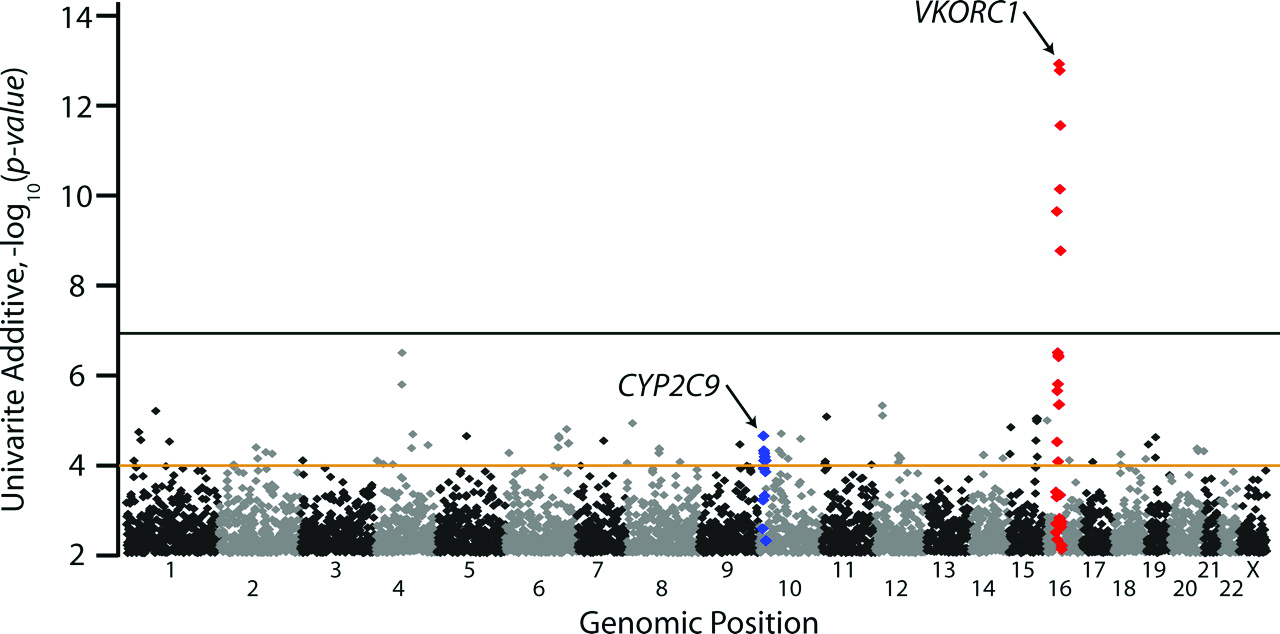
\includegraphics[height=8cm]{GWAS-warfarin.eps}
\end{center}
  \caption{$P$-values from a genome-wide analysis of the association
    between SNP genotype and warfarin dose. The black line is the
    genome-wide level for statistical significance, $10^{-7}$, and the
    brown line is the level, $10^{-4}$ at which SNPs identified in the
    index population were investigated in replicate
    populations~(from~\cite{Cooper-etal-2008}).}\label{fig:GWAS-warfarin}
\end{figure}

\subsection*{Case-control study}

The GWAS approach I just described works well if the trait we're
studying is continuous,\footnote{With the caveats about interpreting
  the association that I mentioned earlier.} but what do we do if the
trait we're interested occurs in only two states, e.g., diseased
vs. healthy? Let's suppose we have a set of ``candidate'' loci, i.e.,
loci that we have some reason to suspect might be related to
expression of the trait. Now let's suppose we divide our population
sample into two different sets: the ``cases,'' i.e., those that have
the disease,\footnote{Please note that I'm using the phrase ``have the
  disease'' merely because it's convenient. Most of the applications
  of this approach have involved investigations of human disease, but
  the approach can be used for {\it any\/} binary phenotype, in which
  case the phrase ``have the disease'' can be replaced with the phrase
  ``have the phenotype of interest.''} and the ``controls,'' i.e.,
those that don't have the disease. Let's further assume that each of
our candidate loci has only two alleles.\footnote{Just as with GWAS,
  this is a reasonable assumption, since we are probably dealing with
  SNP markers.} Then for each of our candidate loci we can estimate
the allele frequency for the population of cases, $p_{case}$, and for
the population of controls, $p_{control}$. Then we simply ask, do we
have evidence that $p_{case}$ is different from $p_{control}$. If so,
we have evidence that allelic differences at this locus are associated
with different probabilities of falling into the case category, i.e.,
allelic differences at this locus are associated with a gene that
influences development of the phenotype. As with our GWAS analysis, we
have to be careful in interpreting this association. It {\it might\/}
reflect physical linkage between the candidate locus and the gene
influencing phenotypic development or it might reflect nothing more
than a statistical association.

\section*{A digression into two-locus population
  genetics\footnote{{\bf Note}: We'll go over only a small part of
  this section in lecture. I'm providing all the details here so you
  can find them in the future if you ever need them.}}

It's pretty obvious that if two loci are on the same chromosome and
tightly linked, alleles at those loci are likely to be statistically
associated with one another, but let's take a closer look at what
being statistically associated means. We'll see that while tight
physical linkage generally implies statistical association, the
reverse isn't true{\dash}unless you have carefully controlled for
other factors that can produce a statistical association.

One of the most important properties of a two-locus system is that it
is no longer sufficient to talk about allele frequencies alone, even
in a population that satisfies all of the assumptions necessary for
genotypes to be in Hardy-Weinberg proportions at each locus. To see
why consider this. With two loci and two alleles there are four
possible gametes:\footnote{Think of drawing the Punnett square for a
  dihybrid cross, if you want.}\index{two-locus genetics!gamet frequenies}

\begin{center}
\begin{tabular}{lcccc}
Gamete    & $A_1B_1$ & $A_1B_2$ & $A_2B_1$ & $A_2B_2$ \\
Frequency & $x_{11}$ & $x_{12}$ & $x_{21}$ & $x_{22}$
\end{tabular}
\end{center}

If alleles are arranged randomly into gametes then,
\begin{eqnarray*}
x_{11} &=& p_1p_2 \\
x_{12} &=& p_1q_2 \\
x_{21} &=& q_1p_2 \\
x_{22} &=& q_1q_2 \quad ,
\end{eqnarray*}
where $p_1 = \hbox{freq}(A_1)$ and $p_2 = \hbox{freq}(A_2)$. But
alleles need not be arranged randomly into gametes. They may covary so
that when a gamete contains $A_1$ it is more likely to contain $B_1$
than a randomly chosen gamete, or they may covary so that a gamete
containing $A_1$ is less likely to contain $B_1$ than a randomly
chosen gamete. This covariance could be the result of the two loci
being in close physical association, but as we'll see in a little bit,
it doesn't have to be. Whenever the alleles covary within gametes
\begin{eqnarray*}
x_{11} &=& p_1p_2 + D \\
x_{12} &=& p_1q_2 - D \\
x_{21} &=& q_1p_2 - D \\
x_{22} &=& q_1q_2 + D \quad ,
\end{eqnarray*}
where $D = x_{11}x_{22} - x_{12}x_{22}$ is known as the {\it gametic
  disequilibrium}.\footnote{You will usually see $D$ referred to as
  the linkage disequilibrium. I think that's misleading. Alleles at
  different loci may be non-randomly associated even when they are not
  physically linked.} When $D \ne 0$ the alleles within gametes
covary, and $D$ measures {\it statistical\/} association between
them. It does not (directly) measure the {\it physical\/}
association. Similarly, $D = 0$ does not imply that the loci are
unlinked, only that the alleles at the two loci are arranged into
gametes independently of one another.\index{gametic
  disequilibrium}\index{two-locus genetics!gametic
  disequilibrium}\index{linkage disequilibrium}

\subsection*{A little diversion}

It probably isn't obvious why we can get away with only one $D$ for
all of the gamete frequencies. The short answer is:
\begin{quote}There are four gametes. That means we need three
  parameters to describe the four frequencies. $p_1$ and $p_2$ are
  two. $D$ is the third.
\end{quote}
Another way is to do a little algebra to verify that the definition is
self-consistent.
\begin{eqnarray*}
D &=& x_{11}x_{22} - x_{12}x_{21} \\
  &=& (p_1p_2 + D)(q_1q_2 + D) - (p_1q_2 - D)(q_1p_2 - D) \\
  &=& \left(p_1q_1p_2q_2 + D(p_1p_2 + q_1q_2) + D^2\right) \\
  && \quad - \left(p_1q_1p_2q_2 - D(p_1q_2 + q_1p_2) + D^2\right) \\
  &=& D(p_1p_2 + q_1q_2 + p_1q_2 + q_1p_2) \\
  &=& D\left(p_1(p_2 + q_2) + q_1(q_2 + p_2)\right) \\
  &=& D(p_1 + q_1) \\
  &=& D \quad.
\end{eqnarray*}

\subsection*{$D$ in a finite population}

In the absence of mutation, $D$ will eventually decay to 0, although
the course of that decay isn't as regular as what is shown in the
Appendix~\cite{Hill-Robertson-1968}. If we allow recurrent mutation at
both loci, however, where\index{two-locus
  genetics!drift}\index{gametic disequilibrium!drift}
\[
\begin{array}{ccccccc}
    &\mu_1            &     &      &     &\mu_2 \\
A_1 &\rightleftharpoons& A_2 &\qquad& B_1 &\rightleftharpoons& B_2
\quad , \\
    &\nu_1            &     &      &     &\nu_2
\end{array}
\]
then it can be shown~\cite{Ohta-Kimura-1969} that the expected value
of $D^2/p_1(1-p_1)p_2(1-p_2)$ is
{\scriptsize
\begin{eqnarray*}
\frac{\mbox{E}(D^2)}{\mbox{E}(p_1(1-p_1)p_2(1-p_2))}
&=& \frac{1}{3 + 4N_e(r+\mu_1+\nu_1+\mu_2+\nu_2)
                           - \frac{2}{(2.5 + N_e(r+\mu_1+\nu_1+\mu_2+\nu_2)
                              + N_e(\mu_1+\nu_1+\mu_2+\nu_2))}} \\
&\approx& \frac{1}{3 + 4N_er} \quad .
\end{eqnarray*}}
Bottom line: In a finite population, we don't expect $D$ to go to 0,
and the magnitude of $D^2$ is inversely related to amount of
recombination between the two loci. The less recombination there is
between two loci, i.e., the smaller $r$ is, the larger the value of
$D^2$ we expect.

This has all been a long way\footnote{OK. You can say it. A {\bf\it
    very\/} long way.} of showing that our initial intuition is
correct. If we can detect a statistical association between a marker
locus and a phenotypic trait, it suggests that the marker locus and a
locus influence expression of the trait are physically linked. {\it
  But\/} we have to account for the effect of population structure,
{\it and\/} we have to account for the effect of {\it past\/}
population structure. Notice also that if the effective population
size is large, $D^2$ may be very small unless $r$ is very small,
meaning that you may need to have a very dense genetic map to detect
any association between any of your marker loci and loci that
influence the trait you're studying. As shown in the Appendix, it
takes a while for the statistical association between loci to decay
after two distinct populations mix. So if we are dealing with
populations having a history of hybridization, teasing apart physical
linkage and statistical association can become very
challenging.\footnote{Think about what this means for GWAS or
  case-control studies in human populations.}

\section*{Population structure with two loci}

You can probably guess where this is going. With one locus I showed
you that there's a deficiency of heterozygotes in a combined sample
even if there's random mating within all populations of which the
sample is composed. The two-locus analog is that you can have gametic
disequilibrium in your combined sample even if the gametic
disequilibrium is zero in all of your constituent
populations. Table~\ref{table:d-structure} provides a simple numerical
example involving just two populations in which the combined sample
has equal proportions from each population.\index{Wahlund effect!two loci}

\begin{table}
\begin{center}
\begin{tabular}{c|cccc|cc|c}
\hline\hline
           & \multicolumn{4}{c|}{Gamete frequencies}
           & \multicolumn{2}{c|}{Allele frequencies} \\
Population & $A_1B_1$ & $A_1B_2$ & $A_2B_1$ & $A_2B_2$
           & $p_{i1}$ & $p_{i2}$ & $D$ \\
\hline
1          & 0.24     & 0.36     & 0.16    & 0.24
           & 0.60     & 0.40     & 0.00 \\
2          & 0.14     & 0.56     & 0.06    & 0.24
           & 0.70     & 0.20     & 0.00 \\
Combined   & 0.19     & 0.46     & 0.11    & 0.24
           & 0.65     & 0.30     & -0.005 \\
\hline
\end{tabular}
\end{center}
\caption{Gametic disequilibrium in a combined population
  sample.}\label{table:d-structure}
\end{table}

\subsection*{The gory details}

You knew that I wouldn't be satisfied with a numerical example, didn't
you? You knew there had to be some algebra coming, right? Well, here
it is. Let
\begin{eqnarray*}
D_i &=& x_{11,i} - p_{1i}p_{2i} \\
D_t &=& \bar x_{11} - \bar p_1\bar p_2 \quad ,
\end{eqnarray*}
where $\bar x_{11} = \frac{1}{K} \sum_{k=1}^K x_{11,k}$, $\bar p_1 =
\frac{1}{K} \sum_{k=1}^K p_{1k}$, and $\bar p_2 = \frac{1}{K}
\sum_{k=1}^K p_{2k}$. Given these definitions, we can now calculate
$D_t$.
\begin{eqnarray*}
D_t &=& \bar x_{11} - \bar p_1\bar p_2 \\
    &=& \frac{1}{K} \sum_{k=1}^K x_{11,k} - \bar p_1\bar p_2 \\
    &=& \frac{1}{K} \sum_{k=1}^K (p_{1k}p_{2k} + D_k) - \bar p_1\bar p_2 \\
    &=& \frac{1}{K} \sum_{k=1}^K (p_{1k}p_{2k} - \bar p_1\bar p_2) + \bar D \\
    &=& \mbox{Cov}(p_1, p_2) + \bar D \quad ,
\end{eqnarray*}
where $\mbox{Cov}(p_1, p_2)$ is the covariance in allele frequencies
across populations and $\bar D$ is the mean within-population gametic
disequilibrium. Suppose $D_i = 0$ for all subpopulations. Then $\bar D
= 0$, too (obviously). But that means that
\begin{eqnarray*}
D_t &=& \hbox{Cov}(p_1, p_2) \quad .
\end{eqnarray*}
So if allele frequencies covary across populations, i.e.,
$\mbox{Cov}(p_1, p_2) \ne 0$, then there will be non-random
association of alleles into gametes in the sample, i.e., $D_t \ne 0$,
even if there is random association alleles into gametes within each
population.\footnote{Well, duh! Covariation of allele frequencies
  across populations means that alleles are non-randomly associated
  across populations. What other result could you possibly expect?}

Returning to the example in Table~\ref{table:d-structure}
\begin{eqnarray*}
\mbox{Cov}(p_1, p_2) &=& 0.5(0.6-0.65)(0.4-0.3) + 0.5(0.7-0.65)(0.2-0.3) \\
                     &=& -0.005 \\
\bar x_{11}          &=& (0.65)(0.30) - 0.005 \\
                     &=& 0.19 \\
\bar x_{12}          &=& (0.65)(0.7) + 0.005 \\
                     &=& 0.46 \\
\bar x_{21}          &=& (0.35)(0.30) + 0.005 \\
                     &=& 0.11 \\
\bar x_{22}          &=& (0.35)(0.70) - 0.005 \\
                     &=& 0.24 \quad .
\end{eqnarray*}

\bibliography{popgen}
\bibliographystyle{plain}

\section*{Appendix: Transmission genetics with two loci}

I'm going to construct a reduced version of a mating table to see how
gamete frequencies change from one generation to the next. There are
ten different two-locus genotypes (if we distinguish coupling,
$A_1B_1/A_2B_2$, from repulsion, $A_1B_2/A_2B_1$, heterozygotes as we
must for these purposes). So a full mating table would have 100
rows. If we assume all the conditions necessary for genotypes to be in
Hardy-Weinberg proportions apply, however, we can get away with just
calculating the frequency with which any one genotype will produce a
particular gamete.\footnote{We're assuming random union of {\it
    gametes\/} rather than random mating of {\it
    genotypes}.}\index{two-locus genetics!transmission}

\begin{center}
\begin{tabular}{lccccc}
\hline\hline
         &           & \multicolumn{4}{c}{Gametes} \\
Genotype & Frequency & $A_1B_1$ & $A_1B_2$ & $A_2B_1$ & $A_2B_2$ \\
\hline
$A_1B_1/A_1B_1$ & $x_{11}^2$ & 1 & 0 & 0 & 0 \\
$A_1B_1/A_1B_2$ & $2x_{11}x_{12}$ & $\half$ & $\half$ & 0 & 0 \\
$A_1B_1/A_2B_1$ & $2x_{11}x_{21}$ & $\half$ & 0 & $\half$ & 0 \\
$A_1B_1/A_2B_2$ & $2x_{11}x_{22}$ & \oneminus & \rhalf & \rhalf & \oneminus \\
$A_1B_2/A_1B_2$ & $x_{12}^2$ & 0 & 1 & 0 & 0 \\
$A_1B_2/A_2B_1$ & $2x_{12}x_{21}$ & \rhalf & \oneminus & \oneminus & \rhalf \\
$A_1B_2/A_2B_2$ & $2x_{12}x_{22}$ & 0 & $\half$ & 0 & $\half$ \\
$A_2B_1/A_2B_1$ & $x_{21}^2$ & 0 & 0 & 1 & 0 \\
$A_2B_1/A_2B_2$ & $2x_{21}x_{22}$ & 0 & 0 & $\half$ & $\half$ \\
$A_2B_2/A_2B_2$ & $x_{22}^2$ & 0 & 0 & 0 & 1 \\
\hline
\end{tabular}
\end{center}

\subsection*{Where do $\frac{1-r}{2}$ and $\frac{r}{2}$ come from?}

Consider the coupling double heterozygote, $A_1B_1/A_2B_2$. When
recombination doesn't happen, $A_1B_1$ and $A_2B_2$ occur in equal
frequency ($1/2$), and $A_1B_2$ and $A_2B_1$ don't occur at all. When
recombination happens, the four possible gametes occur in equal
frequency ($1/4$). So the recombination frequency,\footnote{The
  frequency of recombinant gametes in double heterozygotes.} $r$, is
half the crossover frequency,\footnote{The frequency of cytological
  crossover during meiosis.} $c$, i.e., $r = c/2$. Now the results of
crossing over can be expressed in this table:\index{two-locus genetics!recombination}\index{recombination frequency}

\begin{center}
\begin{tabular}{c|cccc}
\hline\hline
Frequency & $A_1B_1$ & $A_1B_2$ & $A_2B_1$ & $A_2B_2$ \\
\hline
$1-c$     & $\half$  & 0        & 0        & $\half$ \\
$c$       & $\quarter$ & $\quarter$ & $\quarter$ & $\quarter$ \\
\hline
Total     & $\frac{2-c}{4}$ & $\frac{c}{4}$ & $\frac{c}{4}$
          & $\frac{2-c}{4}$ \\
          & $\frac{1-r}{2}$ & $\frac{r}{2}$ & $\frac{r}{2}$
          & $\frac{1-r}{2}$ \\
\hline
\end{tabular}
\end{center}

\subsection*{Changes in gamete frequency}

We can use the mating table table as we did earlier to calculate the
frequency of each gamete in the next generation. Specifically,
\begin{eqnarray*}
x_{11}' &=& x_{11}^2 + x_{11}x_{12} + x_{11}x_{21} + (1-r)x_{11}x_{22}
            + rx_{12}x_{21} \\
        &=& x_{11}(x_{11} + x_{12} + x_{21} + x_{22})
            - r(x_{11}x_{22} - x_{12}x_{21}) \\
        &=& x_{11} - rD \\
x_{12}' &=& x_{12} + rD \\
x_{21}' &=& x_{21} + rD \\
x_{22}' &=& x_{22} - rD \quad .
\end{eqnarray*}

\subsection*{No changes in allele frequency}

We can also calculate the frequencies of $A_1$ and $B_1$ after this
whole process:
\begin{eqnarray*}
p_1' &=& x_{11}' + x_{12}' \\
     &=& x_{11} - rD + x_{12} + rD \\
     &=& x_{11} + x_{12} \\
     &=& p_1 \\
p_2' &=& p_2 \quad .
\end{eqnarray*}
Since each locus is subject to all of the conditions necessary for
Hardy-Weinberg to apply at a single locus, allele frequencies don't
change at either locus. Furthermore, genotype frequencies at each
locus will be in Hardy-Weinberg proportions. But the two-locus gamete
frequencies change from one generation to the next.\index{two-locus genetics!Hardy-Weinberg}

\subsection*{Changes in $D$}

You can probably figure out that $D$ will eventually become zero, and
you can probably even guess that how quickly it becomes zero depends
on how frequent recombination is. But I'd be astonished if you could
guess exactly how rapidly $D$ decays as a function of $r$.  It takes a
little more algebra, but we can say precisely how rapid the decay will
be.\index{two-locus genetics!decay of disequilibrium}
\begin{eqnarray*}
D' &=& x_{11}'x_{22}' - x_{12}'x_{21}' \\
   &=& (x_{11} - rD)(x_{22} - rD) - (x_{12} + rD)(x_{21} + rD) \\
   &=& x_{11}x_{22} - rD(x_{11} + x_{12}) + r^2D^2
       - (x_{12}x_{21} + rD(x_{12} + x_{21}) + r^2D^2) \\
   &=& x_{11}x_{22} - x_{12}x_{21} - rD(x_{11} + x_{12} + x_{21} + x_{22}) \\
   &=& D - rD \\
   &=& D(1-r)
\end{eqnarray*}
Notice that even if loci are unlinked, meaning that $r = 1/2$, $D$
does not reach 0 immediately. That state is reached only
asymptotically. The two-locus analogue of Hardy-Weinberg is that
gamete frequencies will {\it eventually\/} be equal to the product of
their constituent allele frequencies.

\ccLicense

\end{document}




\chapter{Genomic prediction: an {\it extremely\/} brief overview}

Let's review the basic approach we use in genome-wide association
mapping.

\begin{itemize}

\item We measure both the phenotype, $y_i$, of individual $i$ and its
  genotype at a large number of loci, where $x_{ij}$ is the
  individual's genotype at locus $j$.

\item We regress phenotype on genotype one locus at a time, using a
  random effect to correct for phenotypic similarities that reflect
  relatedness rather than similarity in genotype. 
\[
y_i^{(k)} = x_{ij}\beta_j + \phi^{(k)} + \epsilon_i \quad .
\]

\end{itemize}

Keep in mind this is a highly idealized schematic of how GWAS analyses
are actually done.\footnote{Remember, also, that in analyses of human
  disease, a case-control approach is often used rather than the
  regression approach I've been focusing on.} If you want to do GWAS
for real, you should take a look at
GEMMA~(\url{http://www.xzlab.org/software.html})\index{GEMMA} or
TASSEL~(https://www.maizegenetics.net/tassel).\index{TASSEL} One
important way in which what I've presented is a simplification is that
in a real GWAS analysis, you'd estimate the effects of every locus
simultaneously, which raises an interesting problem.

In a typical GWAS analysis\footnote{In humans at least}, you will have
measured the phenotype of a few thousand individuals, but you will
have genotyped those individuals at several hundred thousand
loci. Lango Allen et al.~\cite{LangoAllen-etal-2010}, for example,
report results from a large analysis of height variation in humans,
183,727 individuals genotyped at 2,834,208 loci. What's the problem
here?

There are more predictors~(loci) than observations~(individual
phenotypes). If you remember some basic algebra, you'll remember that
you can't solve a set of linear equations unless you have the same
number of equations as unknowns. For example, you can't solve a set of
three equations that has five unknowns. There's a similar phenomenon
in statistics when we're fitting a linear regression. In statistics we
don't ``solve'' an equation. We find the best fit in a regression, and
we can do so in a reasonable way so long as the number of observations
exceeds the number of variables included in our regression. To put a
little mathematical notation to it, if $n$ is the number of
observations and $p$ is the number of regression parameters we hope to
estimate, life is good (meaning that we can estimate the regression
parameters) so long as $n > p$.\footnote{And the more that $n$ exceeds
  $p$ the better, the more accurate our estimates of the regression
  parameters will be.} The typical situation we encounter in GWAS is
that $n < p$, which means we have to be really sneaky. Essentially
what we do is that we find a way for the data to tell us that a lot of
the parameters don't matter and we fit a regression only to the ones
that do, {\it and\/} we set things up so that the remaining number of
parameters is less than $n$. If that all sounds a little hoky, trust
me it isn't. There are good ways to do it and good statistical
justification for doing it\footnote{And biological justification for
  doing it in GWAS.}, but the mathematics behind it gets pretty hairy,
which is why you want to use GEMMA or TASSEL for a real GWAS. We'll
ignore this part of the challenge associated with GWAS and focus on
another one: complex traits often are influenced by a very large
nubmer of loci. That is, after all, why we started studying
quantitative genetics in the first place.

\section*{Genetics of complex traits}

Let's return to that Lango Allen et al.~\cite{LangoAllen-etal-2010}
GWAS on height in humans. They identified at least 180 loci associated
with differences in height. Moreover, many of the variants are closely
associated with genes that are part of previously identified pathways,
e.g., Hedgehog signaling,\footnote{``The Hedgehog signaling pathway is
  a signaling pathway that transmits information to embryonic cells
  required for proper cell differentiation.''
  \url{https://en.wikipedia.org/wiki/Hedgehog_signaling_pathway},
  accessed 14 August 2021.} or
that were previously identified as being involved in skeletal growth
defects. A more recent study by Wood et al.~\cite{Wood-etal-2014}
synthesized results from 79 studies involving 253,288 individuals and
identified 697 variants that were clustered into 423 loci affecting
differences in height.\footnote{It's worth noting that even this is
  likely to be an underestimate of the number of loci associated with
  height variation in humans because all of the individuals included
  in the analysis were of European ancestry.} Think about what that
means. If you know my genotype at only one of those 697 variants, you
know next to nothing about how tall I am. But what if you knew my
genotype for all of those variants? Then you should be able to do
better.\index{Genome-wide association study!human height}

The basic idea is fairly simple. When you do a full GWAS and estimate
the effects at every locus simultaneously, you are essentially
performing a multiple regression of phenotype on all of the loci
you've scored simultaenously instead of looking at them one at a
time. In equation-speak,
\[
y_i^{(k)} = \sum_j x_{ij}\beta_j + \phi^{(k)} + \epsilon_i \quad .
\]
Now think a bit more about what that equation means. The $\phi^{(k)}$
and $\epsilon_i$ terms represent random variation, in the first case
variation that is correlated among individuals depending on how
closely related they are and in the second case variation that is
purely random. The term $\sum_j x_{ij}\beta_j$ reflects systematic
effects associated with the genotype of individual $i$. In other
words, if we know individual $i$'s genotype, i.e., if we know $x_{ij}$
we can predict what phenotype it will have, namely
$\mu_i = \sum_j x_{ij}\beta_j$. Although we know there will be
uncertainty associated with this prediction, $\mu_i$ is our best guess
of the phenotype for that individual, i.e., our genomic prediction or
polygenic score. In the case of height in human beings, it turns out
that the loci identified in Wood et al.~\cite{Wood-etal-2014} account
for about 16 percent of variation in height.\footnote{In Europe the
  heritability of height at age 20 is about 80
  percent~\cite{Jelenkovic-etal-2016}.}\index{genomic predictioon}
\index{polygenic score} If we don't have too many groups, we could
refine our estimate a bit further by adding in the group-specific
estimate, $\phi^{(k)}$. Of course when we do so, our prediction is no
longer a {\it genomic\/} predictiion, {\it per se}. It's a genomic
prediction enhanced by non-genetic group information.

\subsection*{A toy example}

To make all of this more concrete, we'll explore a toy example using
the highly simplified one locus at a time approach to GWAS with a
highly simplified example of the multiple regression approach to
GWAS. You'll find the {\tt R} code used to create and analyze this
simple example at
\url{http://darwin.eeb.uconn.edu/eeb348-resources/genomic-prediction.R}
If you {\tt source("genomic-prediction.R")} it will

\begin{itemize}

\item Generate a random dataset with 100 individuals and 20 loci, 5 of
  which influence the phenotype. The effect of one ``1'' allele at
  locus 1 is 1, at locus 2 -1, at locus 3 0.5, at locus 4 -0.5, and at
  locus 5 0.25. The standard deviation of the phenotype around the
  predicted mean is 0.1.

\item Run the locus-by-locus regression for each locus and store the
  results (mean and 95\% credible interval) in ``results.csv'' and
  retain the results in {\tt results}. {\tt results} is sorted in by
  the magnitude of the posterior mean, so that loci with the largest
  estimated effect occur at the top and loci with the smallest effect
  occur at the bottom.

\item Run the multiple regression and store the results in {\tt fit}. 
    
\end{itemize}

If you look at the code, you'll see that I use {\tt stan\_lm()} rather
than using {\tt stan\_lmer()}. That's because I simulate the data without
family structure, so there's no need to include the family random
effect.

Table~\ref{table:single} shows results of the locus by locus analysis
from my run of {\tt genomic-prediction.R}. Your results will vary a
bit, both because the Monte Carlo analysis of the data won't be
precisely the same every time and because the data you generate in the
simulation will be a bit different from the data I generated for this
analysis.

% latex table generated in R 3.5.3 by xtable 1.8-3 package
% Sun Apr 28 11:27:43 2019
\begin{table}[ht]
\centering
\begin{tabular}{rrrr}
  \hline
 & mean & 2.5\% & 97.5\% \\ 
  \hline
locus\_1 & 1.01 & 0.76 & 1.27 \\ 
  locus\_2 & -0.97 & -1.12 & -0.82 \\ 
  locus\_3 & 0.63 & 0.34 & 0.91 \\ 
  locus\_4 & -0.42 & -0.71 & -0.13 \\ 
  locus\_5 & 0.42 & 0.11 & 0.72 \\ 
  locus\_14 & 0.23 & -0.07 & 0.52 \\ 
  locus\_8 & -0.17 & -0.47 & 0.13 \\ 
  locus\_6 & -0.14 & -0.47 & 0.18 \\ 
  locus\_20 & -0.13 & -0.46 & 0.18 \\ 
  locus\_19 & -0.12 & -0.44 & 0.20 \\ 
  locus\_10 & 0.11 & -0.22 & 0.44 \\ 
  locus\_18 & 0.09 & -0.22 & 0.40 \\ 
  locus\_9 & -0.09 & -0.39 & 0.22 \\ 
  locus\_12 & -0.09 & -0.41 & 0.26 \\ 
  locus\_15 & -0.07 & -0.37 & 0.23 \\ 
  locus\_11 & -0.07 & -0.40 & 0.27 \\ 
  locus\_7 & -0.04 & -0.34 & 0.27 \\ 
  locus\_16 & -0.04 & -0.35 & 0.28 \\ 
  locus\_13 & 0.03 & -0.29 & 0.36 \\ 
  locus\_17 & 0.01 & -0.32 & 0.35 \\ 
   \hline
\end{tabular}
\caption{Sample results for locus by locus analysis of genetic
  associations using {\tt genomic-prediction.R}}\label{table:single}
\end{table}

For this simulated data set the 5 loci with the largest estimated
effect are the 5 loci for which I specified an effect, but that isn't
always the case. You may well find that a locus that didn't have a
specified effect is one of the top 5. Furthermore, even though this
time the locus by locus approach picked out the right top 5 loci, {\tt
  locus\_14} has an effect that is quite large, the the credible
interval associated with it only overlaps 0, by a bit. It would be
tempting to think that it is worth investigating further. It wouldn't
be as tempting to look at any of the other loci, but a lot of them
have fairly large effects given that the entire observed range of
phenotypes in this data set is -2.8 to 3.2.

Since you've already run {\tt source("genomic-predicition.R")}, you
can now run {\tt plot\_posterior\_predict(fit\_list[[1]])} to plot
phenotype predictions at locus 1 versus the observed phenotype for
each individual~(Figure~\ref{fig:locus-1}). You can see that there is
a relationship between an individual's genotype at this locus, but you
can also see that it's pretty weak. Compare that to the relationship
between phenotype and genotype at {\tt locus\_17}, though, and you'll
see that the genotype at locus 17 doesn't give you any information
about phenotype while the genotype at locus 1 at least gives you a
little~(Figure~\ref{fig:locus-17}).

\begin{figure}
  \begin{center}
    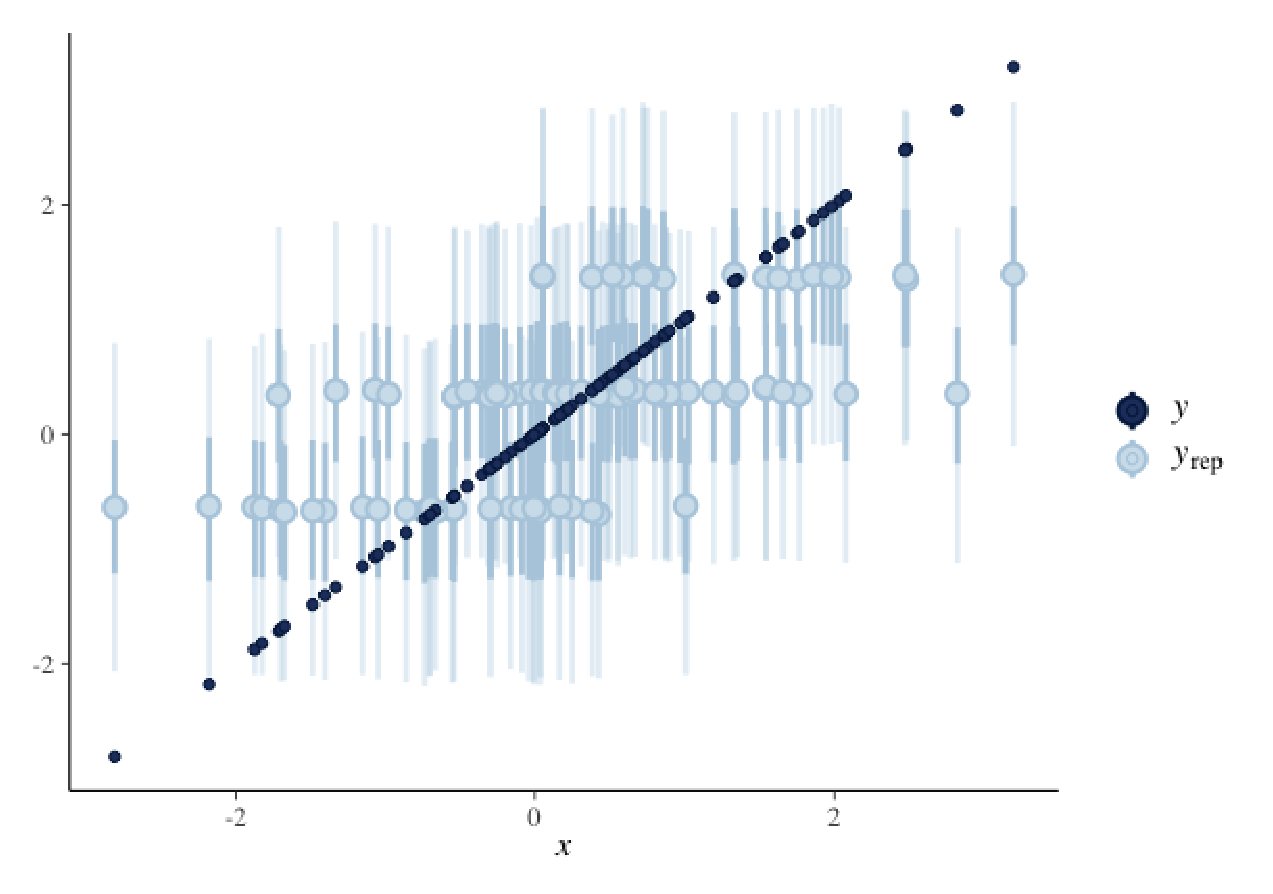
\includegraphics[height=6cm]{genomic-prediction-locus-1.eps}
  \end{center}
  \caption{Posterior prediction for locus 1. Small black dots indicate
    observed phenotypes. Large gray dots indicate the corresponding
    posterior prediction. The darker gray lines show the location of
    50\% credible intervals, and the lighter gray lines show the
    location of 90\% credible intervals.}\label{fig:locus-1}
\end{figure}

\begin{figure}
  \begin{center}
    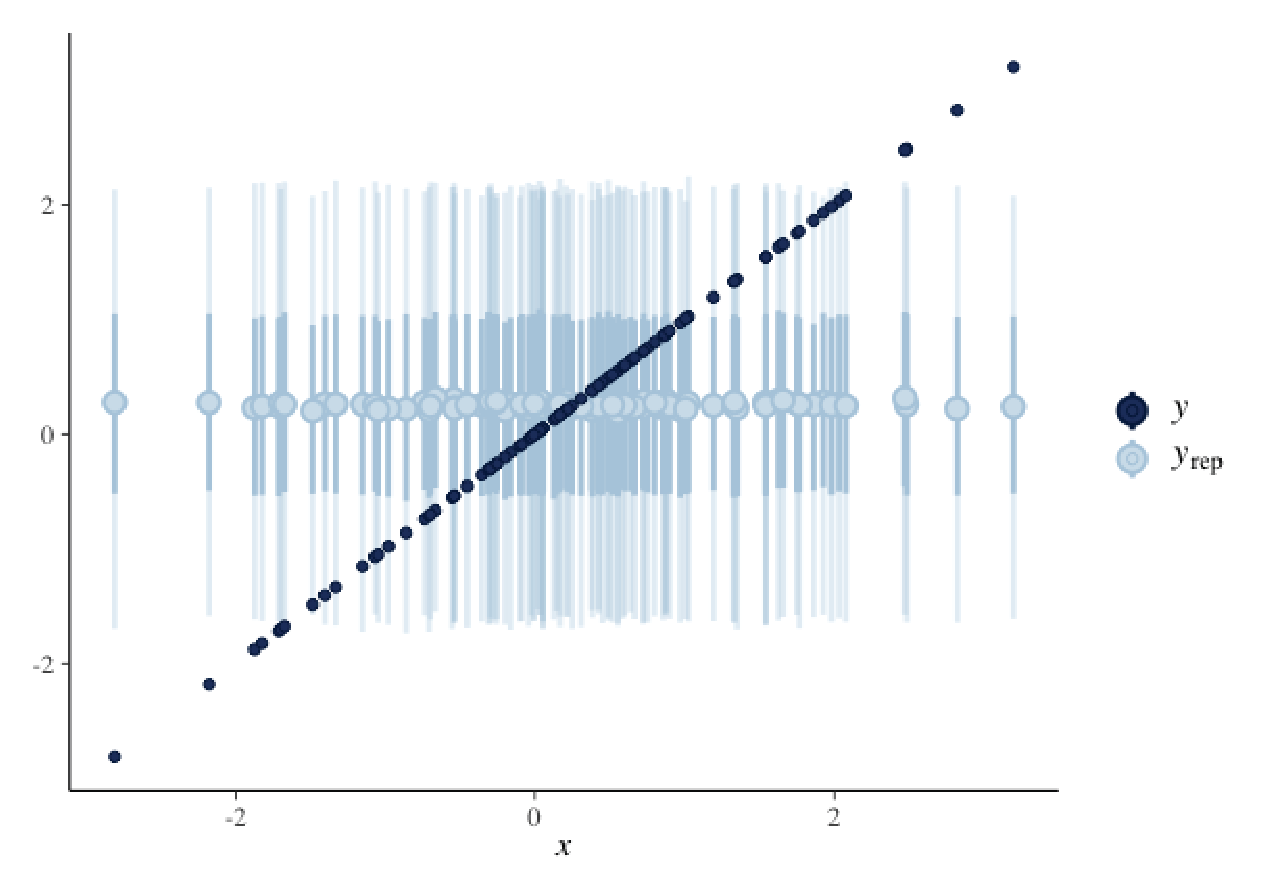
\includegraphics[height=6cm]{genomic-prediction-locus-17.eps}
  \end{center}
  \caption{Posterior prediction for locus 17.}\label{fig:locus-17}
\end{figure}

What about the multiple regression approach? First, take a look at the
estimated effects~(Table~\ref{table:multiple}). Not only does this
approach pick out the right loci, the first five, none of the other
loci have particularly large estimated effects. The largest, {\tt
  locus\_6} and {\tt locus\_8} are both only 0.07, as opposed to 0.14
in the locus by locus analysis. It would take much more extensive
simulation to demonstrate the advantage empirically, but it is clear
from first principles that multiple regression analyses will be more
reliable than locus by locus analyses because a multiple regression
analysis take account of random associations among loci.

Now compare phenotype predictions from the first five loci when each
effect is taken individually from Table~\ref{table:single} with the
prediction derived from the multple regression
approach~(Figure~\ref{fig:multiple}).\footnote{Use {\tt
    compare\_posterior\_predictions(fit\_list[1:5], fit)} to produce a
  similar plot using your results.} As you can see, using all 5 loci
together to predict phenotypes does a very good job of recovering
them. 

\begin{table}[ht]
\centering
\begin{tabular}{rrrr}
  \hline
 & mean & 2.5\% & 97.5\% \\ 
  \hline
locus\_2 & -0.96 & -1.07 & -0.86 \\ 
  locus\_1 & 0.92 & 0.84 & 1.00 \\ 
  locus\_3 & 0.48 & 0.39 & 0.56 \\ 
  locus\_4 & -0.44 & -0.52 & -0.36 \\ 
  locus\_5 & 0.23 & 0.15 & 0.32 \\ 
  locus\_6 & 0.07 & -0.03 & 0.16 \\ 
  locus\_8 & -0.07 & -0.15 & 0.02 \\ 
  locus\_11 & 0.06 & -0.03 & 0.15 \\ 
  locus\_14 & -0.06 & -0.14 & 0.03 \\ 
  locus\_20 & -0.06 & -0.14 & 0.03 \\ 
  locus\_12 & 0.05 & -0.04 & 0.14 \\ 
  locus\_7 & -0.04 & -0.12 & 0.04 \\ 
  locus\_18 & -0.03 & -0.10 & 0.06 \\ 
  locus\_16 & 0.02 & -0.07 & 0.10 \\ 
  locus\_10 & 0.02 & -0.07 & 0.11 \\ 
  locus\_19 & -0.02 & -0.10 & 0.06 \\ 
  locus\_17 & 0.01 & -0.08 & 0.09 \\ 
  locus\_9 & 0.01 & -0.08 & 0.09 \\ 
  locus\_15 & 0.00 & -0.07 & 0.08 \\ 
  locus\_13 & -0.00 & -0.09 & 0.09 \\ 
   \hline
\end{tabular}
\caption{Results from multiple regression analysis of simulated
  data.}\label{table:multiple} 
\end{table}

\begin{figure}
  \begin{center}
    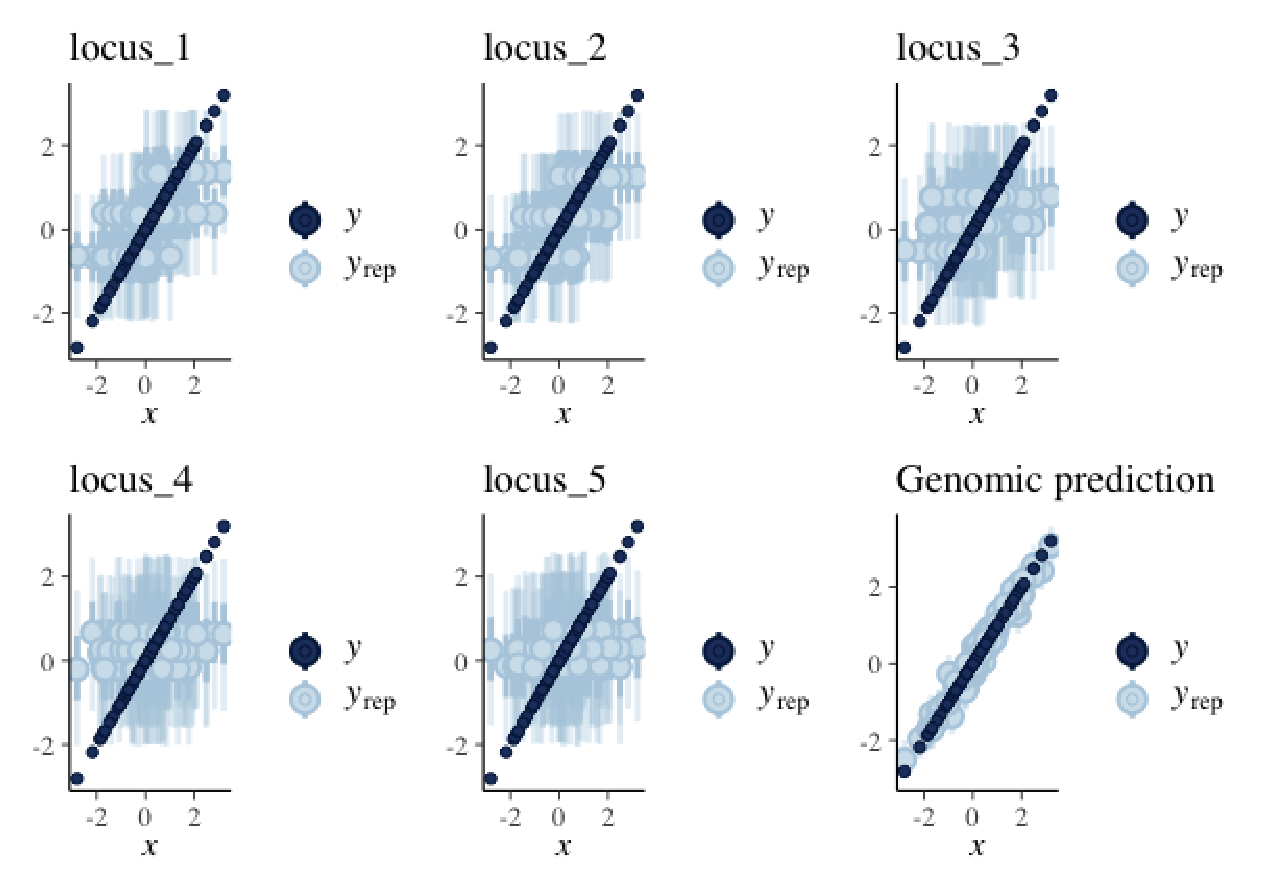
\includegraphics[height=6cm]{genomic-prediction-multiple.eps}
  \end{center}
  \caption{Posterior predictions for loci 1-5 from locus by locus
    regressions and the posterior preduction for the multiple
    regression.}\label{fig:multiple}
\end{figure}

\subsection*{CAUTION: Danger ahead!}\index{genomic prediction!caveats}

This all seems very promising, but a word of caution is in
order. Several papers, including one by Peter Turchin, have suggested
that there is strong evidence for selection on polygenic scores
associated with height using the same data set of 253,288 individuals
I referred to earlier~(references in Berg et
al.~\cite{Berg-etal-2018}). Specifically, these studies suggested (a)
that there is a cline in polygenic scores from south-to-north in
Europe (taller phenotypes predicted in the north) and (b) that the
cline is too steep to be accounted for by neutrual evolution. Berg et
al.~\cite{Berg-etal-2018} re-examined these claims using new data
available from the UK
Biobank~(\url{https://www.bdi.ox.ac.uk/research/uk-biobank}), which
includes a host of information on individual phenotypes as well as
genome-wide genotypes for the 500,000 individuals included in the
sample.\footnote{Although all of the samples are from the UK, one of
  the data sets Berg et al.~\cite{Berg-etal-2018} studied included
  individuals of European, but non-UK, ancestry.} They failed to
detect evidence of a cline in polygenic scores in their
analysis~(Figure~\ref{fig:UK-biobank}).

\begin{figure}
  \begin{center}
    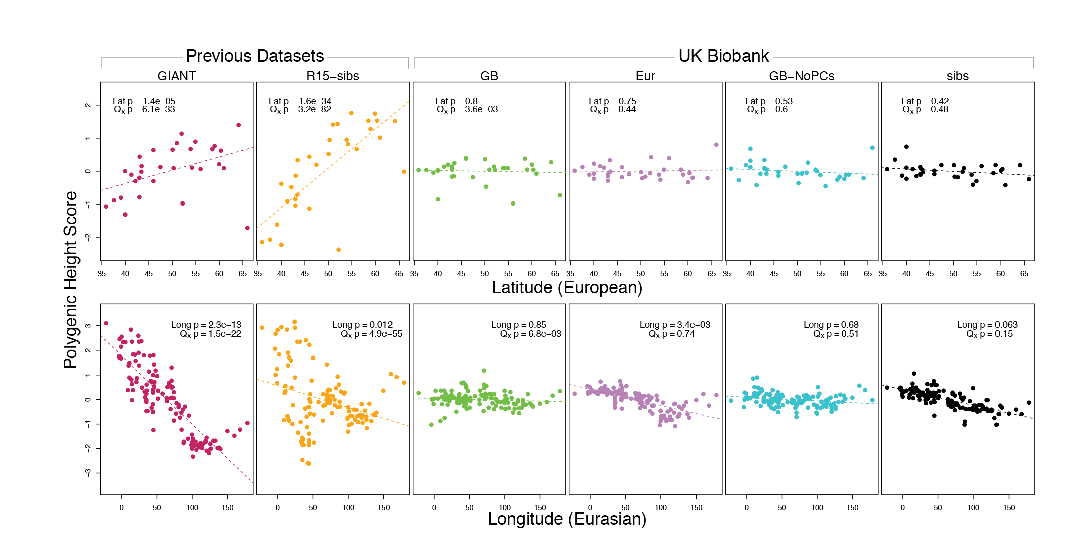
\includegraphics[width=\textwidth]{UK-biobank.eps}
  \end{center}
  \caption{Polygenic score as a function of latitude and longitude for
    several different GWAS data sets.}\label{fig:UK-biobank}
\end{figure}

In thinking about this result, it's important to understand that Berg
et al.~\cite{Berg-etal-2018} did something a bit different from what
we did, but it's exactly what you'd want to do if polygenic scores
worked. They estiamted polygenic scores from each of the data sets
identified in the figure. Then they used those scores to estimate
polygenic scores for a new set of samples derived from the 1000
Genomes and Human Origins projects.\footnote{See Berg et
  al.~\cite{Berg-etal-2018} for details.} Think about it. A polygenic
score doesn't do us a whole lot of good if all it lets us do is to
predict (with uncertainty) a phenotype we already know. The hope is
that we can use the polygenic score to predict phenotypes for
individuals when we know their genotype but not their phenotype. What
this result shows is that extrapolation of a regression beyond the
range of variation included in the sample from which it was estimated
can be very problematic.



\part{Old chapters, no longer updated}

\chapter{Testing Hardy-Weinberg}

Because the Hardy-Weinberg principle tells us what to expect
concerning the genetic composition of a sample when no evolutionary
forces are operating, one of the first questions population
geneticists often ask is ``Are the genotypes in this sample present in
the expected, i.e., Hardy-Weinberg, proportions?'' We ask that
question because we know that if the genotypes are {\it not\/} in
Hardy-Weinberg proportions, at least one of the assumptions underlying
derivation of the principle has been violated, i.e., that there is
some evolutionary force operating on the population, and we know that
we can use the magnitude and direction of the departure to say
something about what those forces might be. In particular, we now know
that inbreeding leads to a deficiency of heterozygotes, and we know
that the extent of that deficiency can be measured by
$f$.\footnote{Quiz question: Which definition of $f$ is relevant for
  determining whether there is a deficiency of heterozygotes?}

What we haven't talked about is (a) how to estimate $f$ from data and
(b) how to tell whether we have good evidence that the estimate is
positive (meaning that there's a deficiency of heterozygotes in the
population) or negative. Both (a) and (b) pose more of a challenge
than you might initially think. After all we also know that the
numbers in our sample may differ from expectation just because of
random sampling error. For example, Table~\ref{table:MN-data} presents
data from a sample of 1000 English blood donors scored for MN
phenotype. M and N are co-dominant, so that heterozygotes can be
distinguished from the two homozygotes. Clearly the observed and
expected numbers don't look very different.\footnote{For the time
  being, I simply calculated the expected numbers in the way you'd
  tell your students in introductory biology to do it: (1) Use the
  sample frequency of M to estimate its population frequency. (This is
  a maximum-likelihood estimate, by the way. (2) Calculate the
  expected frequency of each genotype from the Hardy-Weinberg
  proportions. (3) Calculated the expected numbers of each genotype by
  multiplying the expected frequency of each by the total sample
  size.} The differences semm likely to be attributable purely to
chance, but we need some way of assessing that
``likeliness.''\index{testing Hardy-Weinberg}

\begin{table}
\begin{center}
\begin{tabular}{cccc}
\hline\hline
          &          & Observed & Expected \\
Phenotype & Genotype & Number   & Number   \\
\hline
M         & mm       & 298      & 294.3 \\
MN        & mn       & 489      & 496.3 \\
N         & nn       & 213      & 209.3 \\
\hline
\end{tabular}
\end{center}
\caption{Adapted from Table 2.4 in~\cite{Hedrick-2000}
  (from~\cite{Cleghorn-1960})}\label{table:MN-data}
\end{table}

\section*{Testing Hardy-Weinberg}

One approach to testing the hypothesis that genotypes are in
Hardy-Weinberg proportions is quite simple. We can simply do a
$\chi^2$ or $G$-test for goodness of fit between observed and
predicted genotype (or phenotype) frequencies, where the predicted
genotype frequencies are derived from our estimates of the allele
frequencies in the population.\footnote{If you're not familiar with
  the $\chi^2$ or $G$-test for goodness of fit, consult any
  introductory statistics or biostatistics book, and you'll find a
  description. In fact, you probably don't have to go that far. You
  can probably find one in your old genetics textbook. Or you can just
  boot up your browser and head to Wikipedia:
  \myurl{http://en.wikipedia.org/wiki/Goodness\_of\_fit}. }\index{testing
  Hardy-Weinberg!goodness of fit} There's only one problem. To do
either of these tests we have to know how many degrees of freedom are
associated with the test. How do we figure that out? In general, the
formula is
\begin{eqnarray*}
\hbox{d.f.} &=& (\hbox{\# of categories in the data -1 }) \\
&&- (\hbox{\#
              number of parameters estimated from the data}) \quad .
\end{eqnarray*}
For this problem we have
\begin{eqnarray*}
\hbox{d.f.} &=& (\hbox{\# of phenotype categories in the data - 1}) \\
&&- (\hbox{\# of allele frequencies estimated from the data}) \\
&=& (3-1) - 1 \\
&=& 1 \quad .
\end{eqnarray*}
In the ABO blood group we have 4 phenotype categories, and 3
allele frequencies. That means that a test of whether a particular
data set has genotypes in Hardy-Weinberg proportions will have
$(4-1)-(3-1) = 1$ degrees of freedom for the test. Notice that this
also means that if you have completely dominant markers, like RAPDs or
AFLPs, you can't determine whether genotypes are in Hardy-Weinberg
proportions because you have 0 degrees of freedom available for the
test.

\subsection*{An example}

Table~\ref{table:abo-data} exhibits data drawn from a study of
phenotypic variation among individuals at the ABO blood locus:

\begin{table}
\begin{center}
\begin{tabular}{lccccc}
Phenotype &   A &  AB &   B &   O & Total \\
Observed  & 862 & 131 & 365 & 702 & 2060
\end{tabular}
\end{center}
\caption{Data on variation in ABO blood type.}\label{table:abo-data}
\end{table}
The maximum-likelihood estimate of allele frequencies,
assuming Hardy-Weinberg, is:\footnote{Take my word for it, or run the
  EM algorithm on these data yourself.}
\begin{eqnarray*}
p_a &=& 0.281 \\
p_b &=& 0.129 \\
p_o &=& 0.590 \quad , \\
\end{eqnarray*}
giving expected numbers of 846, 150, 348, and 716 for the
four phenotypes. $\chi^2_1 = 3.8$, $0.05 < p < 0.1$.

\section*{A Bayesian approach}

We've already seen how to use JAGS to provide allele frequency
estimates from phenotypic data at the \htmladdnormallink{ABO
  locus}{http://darwin.eeb.uconn.edu/eeb348/supplements-2014/multinomial.txt}.\index{testing Hardy-Weinberg!Bayesian approach}
\begin{verbatim}
model {
   # likelihood
   pi[1] <- p.a*p.a + 2*p.a*p.o
   pi[2] <- 2*p.a*p.b
   pi[3] <- p.b*p.b + 2*p.b*p.o
   pi[4] <- p.o*p.o
   x[1:4] ~ dmulti(pi[],n)

   # priors
   a1 ~ dexp(1)
   b1 ~ dexp(1)
   o1 ~ dexp(1)
   p.a <- a1/(a1 + b1 + o1)
   p.b <- b1/(a1 + b1 + o1)
   p.o <- o1/(a1 + b1 + o1)

   n <- sum(x[])
}
list(x=c(862, 131, 365, 702))
\end{verbatim}
As you may recall, this produced the following results:
\begin{verbatim}
> source("multinomial.R")
Compiling model graph
   Resolving undeclared variables
   Allocating nodes
   Graph Size: 20

Initializing model

  |++++++++++++++++++++++++++++++++++++++++++++++++++| 100%
  |**************************************************| 100%
Inference for Bugs model at "multinomial.txt", fit using jags,
 5 chains, each with 2000 iterations (first 1000 discarded)
 n.sims = 5000 iterations saved
         mu.vect sd.vect   2.5%    25%    50%    75%  97.5%  Rhat n.eff
p.a        0.282   0.008  0.266  0.276  0.282  0.287  0.297 1.001  5000
p.b        0.129   0.005  0.118  0.125  0.129  0.133  0.140 1.001  5000
p.o        0.589   0.008  0.573  0.584  0.589  0.595  0.606 1.001  5000
deviance  27.811   2.007 25.830 26.363 27.229 28.577 33.245 1.001  4400

For each parameter, n.eff is a crude measure of effective sample size,
and Rhat is the potential scale reduction factor (at convergence, Rhat=1).

DIC info (using the rule, pD = var(deviance)/2)
pD = 2.0 and DIC = 29.8
DIC is an estimate of expected predictive error (lower deviance is better).
>
\end{verbatim}
Now that we know about inbreeding coefficients and that they allow us
to measure the departure of genotype frequencies from Hardy-Weinberg
proportions, we can modify this a bit and estimate allele frequencies
without assuming that genotypes are in Hardy-Weinberg proportions.
\begin{verbatim}
model {
   # likelihood
   pi[1] <- p.a*p.a + f*p.a*(1-p.a) + 2*p.a*p.o*(1-f)
   pi[2] <- 2*p.a*p.b*(1-f)
   pi[3] <- p.b*p.b + f*p.b*(1-p.b) + 2*p.b*p.o*(1-f)
   pi[4] <- p.o*p.o + f*p.o*(1-p.o)
   x[1:4] ~ dmulti(pi[],n)

   # priors
   a1 ~ dexp(1)
   b1 ~ dexp(1)
   o1 ~ dexp(1)
   p.a <- a1/(a1 + b1 + o1)
   p.b <- b1/(a1 + b1 + o1)
   p.o <- o1/(a1 + b1 + o1)

   f ~ dunif(0,1)

   n <- sum(x[])
}
\end{verbatim}
This simple change produces the following results:
\begin{verbatim}
> source("abo-inbreeding.R")
Compiling model graph
   Resolving undeclared variables
   Allocating nodes
   Graph Size: 30

Initializing model

  |++++++++++++++++++++++++++++++++++++++++++++++++++| 100%
  |**************************************************| 100%
Inference for Bugs model at "abo-inbreeding.txt", fit using jags,
 5 chains, each with 2000 iterations (first 1000 discarded)
 n.sims = 5000 iterations saved
         mu.vect sd.vect   2.5%    25%    50%    75%  97.5%  Rhat n.eff
f          0.403   0.139  0.059  0.326  0.429  0.505  0.599 1.013   550
p.a        0.349   0.027  0.290  0.332  0.352  0.368  0.392 1.006   960
p.b        0.161   0.014  0.132  0.152  0.162  0.171  0.186 1.006   840
p.o        0.490   0.039  0.429  0.461  0.485  0.514  0.577 1.006  1000
deviance  25.200   2.416 22.249 23.411 24.716 26.342 31.206 1.007   470

For each parameter, n.eff is a crude measure of effective sample size,
and Rhat is the potential scale reduction factor (at convergence, Rhat=1).

DIC info (using the rule, pD = var(deviance)/2)
pD = 2.9 and DIC = 28.1
DIC is an estimate of expected predictive error (lower deviance is better).
>
\end{verbatim}
Notice that the allele frequency estimates have changed quite a bit
and that the posterior mean of $f$ is about 0.40. On first appearance,
that would seem to indicate that we have lots of inbreeding in this
sample. {\bf BUT} it's a human population. It doesn't seem very
likely that a human population is really that highly inbred.

Indeed, take a closer look at {\it all\/} of the information we have
about that estimate of $f$. The 95\% credible interval for $f$ is
between 0.06 and 0.60. That suggests that we don't have much
information at all about $f$ from these data.\footnote{That shouldn't
  be too surprising, since any information we have about $f$ comes
  indirectly through our allele frequency estimates.} How can we tell
if the model with inbreeding is better than the model that assumes
genotypes are in Hardy-Weinberg proportions?

\subsection*{The Deviance Information Criterion}

A widely used statistic for comparing models in a Bayesian framework
is the Deviance Information Criterion.\index{Deviance Information
  Criterion} {\tt R2jags} calculates an estimate of it for us
automatically, but you need to know that if you're serious about model
comparison, yous shouldn't rely on the DIC calculation from {\tt
  R2jags} unless you've verified it.\footnote{If you're interested in
  learning more, feel free to ask, but I'm afraid both the explanation
  and the solution are a little complicated.} Fortunately, in this
case, the results are fairly reliable.\footnote{You'll just have to
  trust me on this unless you asked the last question.} The
results of the DIC calculations for our two models are summarized in
Table~\ref{table:ABO-dic}.

\begin{table}
\begin{center}
\begin{tabular}{c|ccc}
\hline\hline
Model   & deviance & pD    & DIC \\
\hline
$f > 0$ & 25.2 & 2.9 & 28.1 \\
$f = 0$ & 27.8 & 2.0 & 29.9 \\
\hline
\end{tabular}
\end{center}
\caption{DIC calculations for the ABO example.}\label{table:ABO-dic}
\end{table}

The {\tt deviance} is a measure of how well the model fits the data,
specifically -2 times the average of the log likelihood values
calculated from the parameters in each sample from the posterior. {\tt
  pD} is a measure of model complexity, roughly speaking the number of
parameters in the model.\footnote{Notice that we estimated 2
  parameters in the $f=0$ model (2 allele frequencies) and 3
  parameters in the $f>0$ model (2 allele frequencies plus the
  inbreeding coefficient).} DIC is a composite measure of how well the
model does. It's a compromise between fit and complexity, and smaller
DICs are preferred. A difference of more than 7-10 units is regarded
as strong evidence in favor of the model with the smaller DIC.

In this case the difference in DIC values is only about 0.8, so we
have very little evidence for $f > 0$ model for these data. This is
consistent with the weak evidence for a departure from Hardy-Weinberg
that was revealed in the $\chi^2$ analysis.


\input{genetic-structure-hierarchy}
\input{nca}
\input{migrate-ima.tex}
\chapter{Approximate Bayesian Computation}

Lacey Knowles studied grasshoppers in the genus {\it Melanopus}. She
collected 1275bp of DNA sequence data from cytochrome oxidase I (COI)
from 124 individuals of {\it M. oregonensis\/} and two outgroup
speices. The specimens were collected from 15 ``sky-island'' sites in
the northern Rocky Mountains~(see Figure~\ref{fig:sky-islands};
\cite{Knowles-2001}). Two alternative hypotheses had been proposed to
describe the evolutionary relationships among these
grasshoppers~(refer to Figure~\ref{fig:divergence-hypotheses} for a
pictorial representation):\index{Melanopus@\textit{Melanopus}}

\begin{figure}
\begin{center}
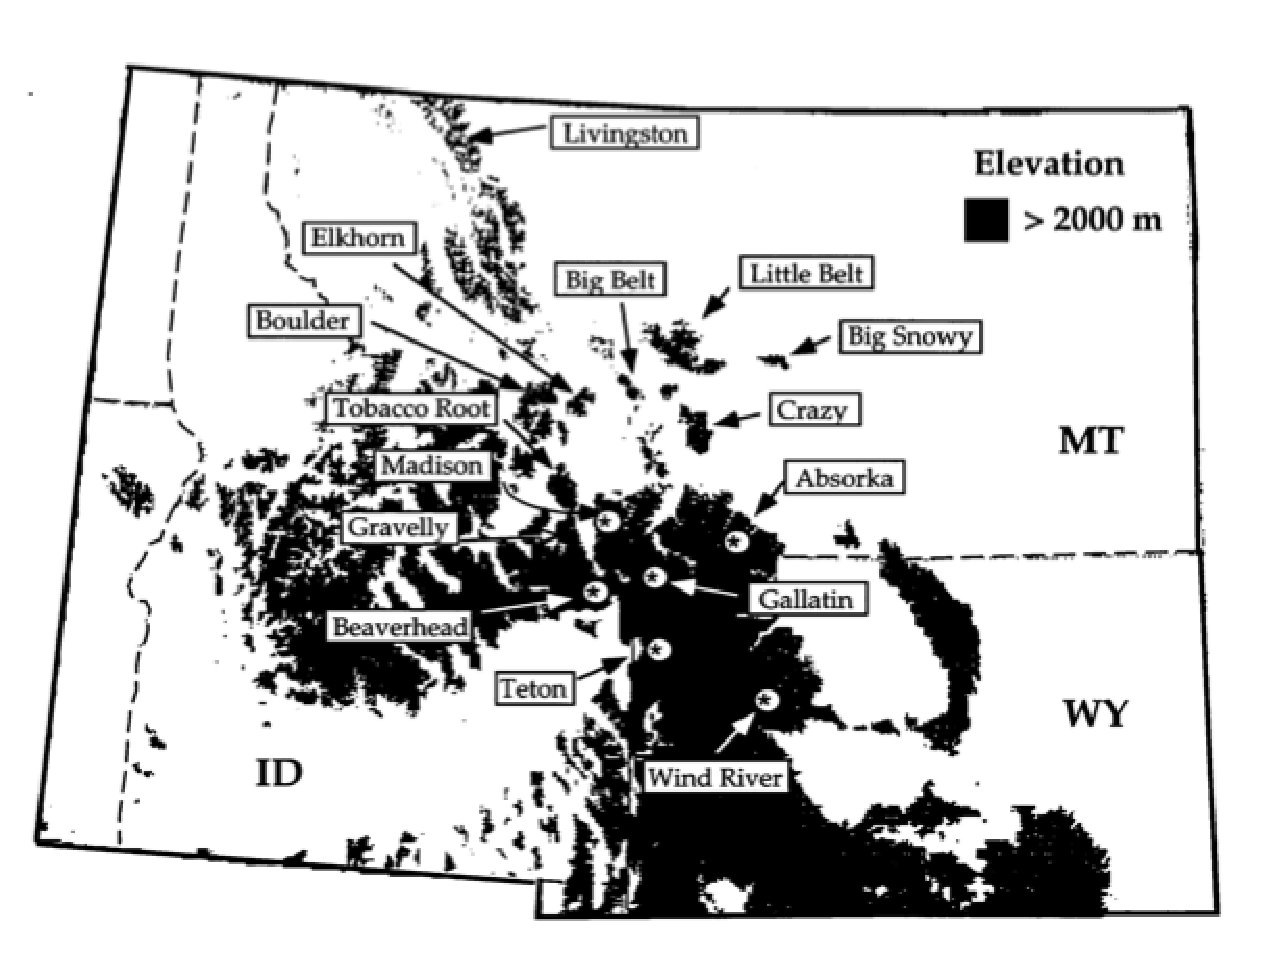
\includegraphics[height=6cm]{sky-islands.eps}
\end{center}
\caption{Collection sites for {\it Melanopus oregonensis\/} in the
  northern Rocky Mountains~(from~\cite{Knowles-2001}).}\label{fig:sky-islands}
\end{figure}

\begin{itemize}

\item {\bf Widespread ancestor}: The existing populations might represent
  independently derived remnants of a single, widespread
  population. In this case all of the populations would be equally
  related to one another.

\item {\bf Multiple glacial refugia}: Populations that shared the same
  refugium will be closely related while those that were in different
  refugia will be distantly related.

\end{itemize}

\begin{figure}
\begin{center}
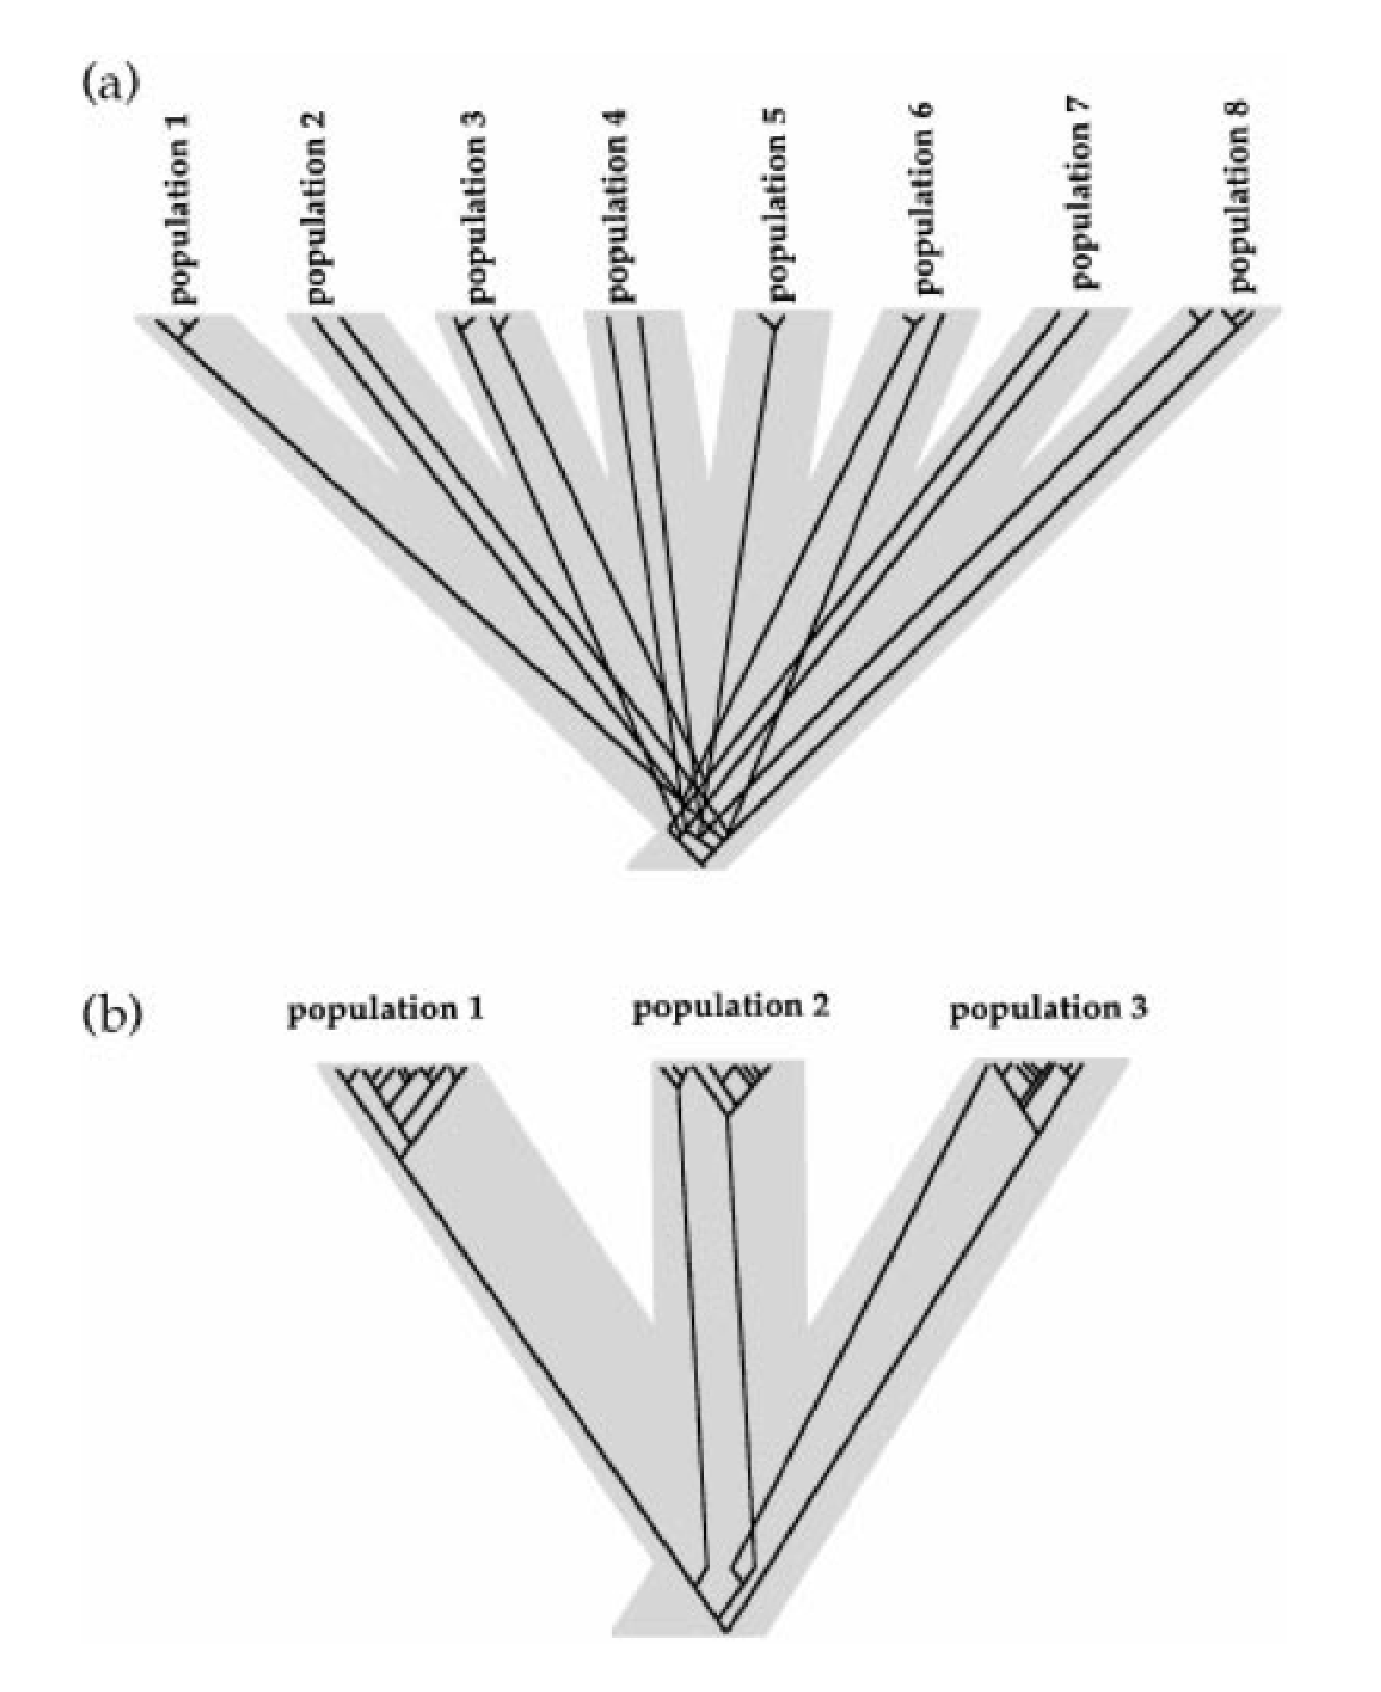
\includegraphics[height=6cm]{divergence-hypotheses.eps}
\end{center}
\caption{Pictorial representations of the ``widespread ancestor''
  (top) and ``glacial refugia'' (bottom)
  hypotheses~(from~\cite{Knowles-2001}).}\label{fig:divergence-hypotheses}
\end{figure}

As is evident from Figure~\ref{fig:divergence-hypotheses}, the two
hypotheses have very different consequences for the coalescent history
of alleles in the sample. Since the interrelationships between
divergence times and time to common ancestry differ so markedly
between the two scenarios, the pattern of sequence differences found
in relation to the geographic distribution will differ greatly between
the two scenarios. 

Using techniques described in Knowles and
Maddison~\cite{Knowles-Maddison-2002}, Knowles simulated gene trees
under the widespread ancestor hypothesis. She then placed them within
a population tree representing the multiple glacial refugia hypothesis
and calculated a statistic, $s$, that measures the discordance between
a gene tree and the population tree that contains it. This gave her a
distribution of $s$ under the widespread ancestor hypothesis. She
compared the $s$ estimated from her actual data with this distribution
and found that the observed value of $s$ was only 1/2 to 1/3 the size
of the value observed in her simulations.\footnote{The discrepancy was
  largest when divergence from the widespread ancestor was assumed to
  be very recent.} Let's unpack that a bit. 

\begin{itemize}

\item Knowles estimated the the phylogeny of the haplotypes in her
  sample. $s$ is the estimated minimum number of among-population
  migration events necessary to account for where haplotypes are
  currently found given the inferred
  phylogeny~\cite{Slatkin-Maddison-1989}. Let's call the $s$ estimated
  from the data $s_{obs}$.

\item Then she simulated a neutral coalescence process in which the
  populations were derived from a single, widespread ancestral
  population. For each simulation she rearranged the data so that
  populations were grouped into separate refugia and estimated $s_{sim}$
  from the rearranged data, and she repeated this 100 times for
  several different times since population splitting.

\end{itemize}

\noindent The results are shown in
Figure~\ref{fig:knowles-s-values}. As you can see, the observed $s$
value is much smaller than any of those obtained from the coalescent
simulations. That means that the observed data require far fewer
among-population migration events to account for the observed
geographic distribution of haplotypes than would be expected with
independent origin of the populations from a single, widespread
ancestor. In short, Knowles presented strong evidence that her data
are not consistent with the widespread ancestor
hypothesis.\index{statistical phylogeography!example}

\begin{figure}
\begin{center}
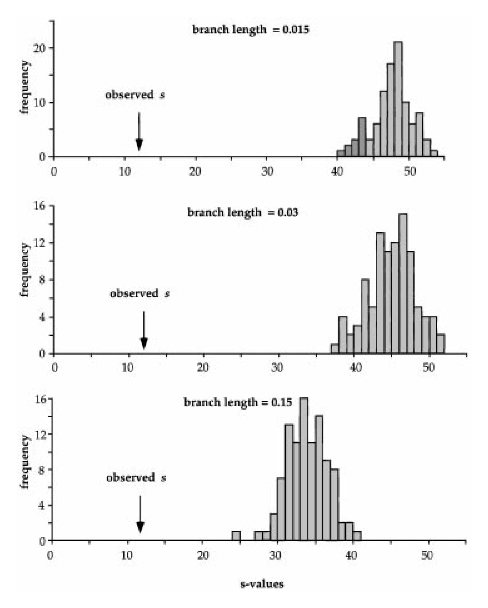
\includegraphics[height=10cm]{knowles-s-values.eps}
\end{center}
\caption{Distribution of the observed minimum number of
  among-population migration events, $s$, and the expected minimum
  number of migration events under the ``widespread ancestor''
  hypothesis.~(from~\cite{Knowles-2001}).}\label{fig:knowles-s-values}
\end{figure}

\section*{Approximate Bayesian computation: motivation}\index{ABC}\index{Approximate Bayesian Computation}

Approximate Bayesian Computation (ABC for short), extends the basic
idea we've just seen to consider more complicated scenarios. The {\tt
  IMa} approach developed by Nielsen, Wakely, and Hey is potentially
{\it very\/} flexible and {\it very\/}
powerful~\cite{Hey-Nielsen-2004,Hey-Nielsen-2007,Nielsen-Wakeley-2001}. It
allows for non-equilibrium scenarios in which the populations from
which we sampled diverged from one another at different times, but
suppose that we think our populations have dramatically increased in
size over time (as in humans) or dramatically changed their
distribution (as with an invasive species). Is there a way to use
genetic data to gain some insight into those processes? Would I be
asking that question if the answer were ``No''?

\section*{An example}

Let's change things up a bit this time and start with an example of a
problem we'd like to solve first. Once you see what the problem is,
then we can talk about how we might go about solving it. The case
we'll discuss is the case of the cane toad, {\it Bufo marinus}, in
Australia.\index{Bufo@\textit{Bufo}!\textit{marinus}}

You may know that the cane toad is native to the American tropics. It
was purposely introduced into Australia in 1935 as a biocontrol agent,
where it has spread across an area of more than 1 million km$^2$. Its
range is still expanding in northern Australia and to a lesser extent
in eastern
Australia~(Figure~\ref{fig:cane-toad-expansion}).\footnote{All of this
  information is from the introduction to~\cite{Estoup-etal-2004}.}
Estoup et al.~\cite{Estoup-etal-2004} collected microsatellite data
from 30 individuals in each of 19 populations along roughly linear
transects in the northern and eastern expansion areas.

\begin{figure}
\begin{center}
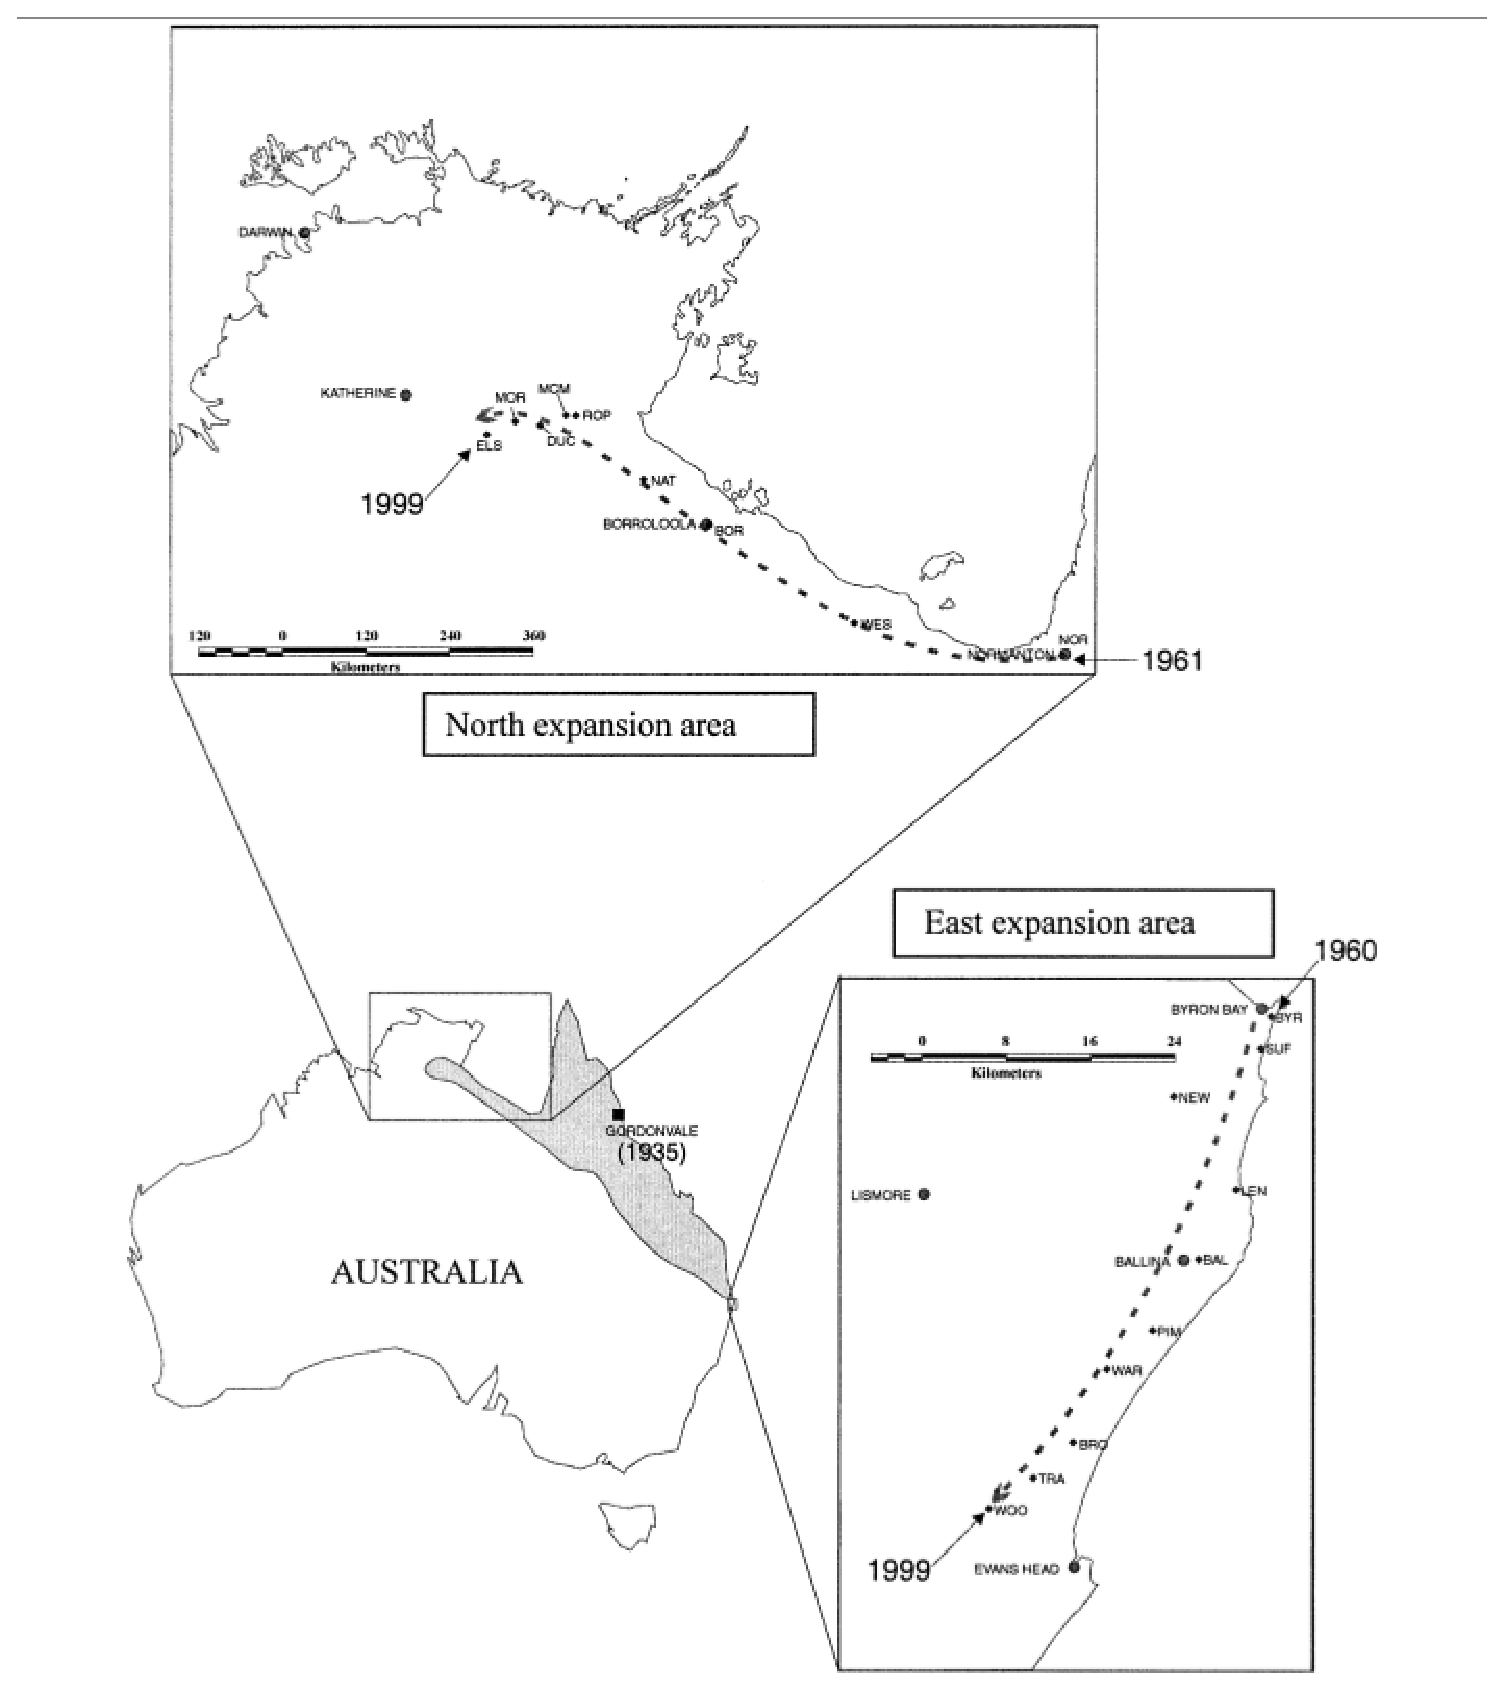
\includegraphics[width=6.0in]{cane-toad-expansion.eps}
\end{center}
\caption{Maps showing the expansion of the cane toad population in
  Australia since its introduction in 1935~(from~\cite{Estoup-etal-2004}).}\label{fig:cane-toad-expansion}
\end{figure}

With these data they wanted to distinguish among five possible
scenarios describing the geographic spread:

\begin{itemize}

\item {\bf Isolation by distance}: As the expansion proceeds, each new
  population is founded by or immigrated into by individuals with a
  probability proportional to the distance from existing populations.

\item {\bf Differential migration and founding}: Identical to the
  preceding model except that the probability of founding a population
  may be different from the probability of immigration into an
  existing population.

\item {\bf ``Island'' migration and founding}: New populations are
  established from existing populations without respect to the
  geographic distances involved, and migration occurs among
  populations without respect to the distances involved.

\item {\bf Stepwise migration and founding with founder events}: Both
  migration and founding of populations occurs only among immediately
  adjacent populations. Moreover, when a new population is
  established, the number of individuals involved may be very small.

\item {\bf Stepwise migration and founding without founder events}:
  Identical to the preceding model except that when a population is
  founded its size is assumed to be equal to the effective population
  size. 

\end{itemize}

That's a pretty complex set of scenarios. Clearly, you could use {\tt
  Migrate} or {\tt IMa2} to estimate parameters from the data Estoup
et al.~\cite{Estoup-etal-2004} report, but would those parameters
allow you to distinguish those scenarios? Not in any straightforward
way that I can see. Neither {\tt Migrate} nor {\tt IMa2} distinguishes
between founding and migration events for example. And with {\tt IMa2}
we'd have to specify the relationships among our sampled populations
before we could make any of the calculations. In this case we want to
test alternative hypotheses of population relationship. So what do we
do?

\section*{Approximate Bayesian Computation}\index{Approximate Bayesian Computation}

Well, in principle we could take an approach similar to what {\tt
  Migrate} and {\tt IMa2} use. Let's start by reviewing what we did
last time\footnote{More accurately, what Peter Beerli, Joe
  Felsenstein, Rasmus Nielsen, John Wakeley, and Jody Hey did.} with
{\tt Migrate} and {\tt IMa2}. In both cases, we knew how to simulate
data given a set of mutation rates, migration rates, local effective
population sizes, and times since divergence. Let's call that whole,
long string of parameters $\xi$ and our big, complicated data set
$X$. If we run enough simulations, we can keep track of how many of
those simulations produce data identical to the data we
collected. With those results in hand, we can estimate $P(X|\xi)$,
the likelihood of the data, as the fraction of simulations that
produce data identical to the data we collected.\footnote{The actual
  implementation is a bit more involved than this, but that's the
  basic idea.} In principle, we could take the same approach in this,
much more complicated, situation. But the problem is that there are an
astronomically large number of different possible coalescent histories
and different allelic configurations possible with any one population
history both because the population histories being considered are
pretty complicated and because the coalescent history of every locus
will be somewhat different from the coalescent history at other
loci. As a result, the chances of getting {\it any\/} simulated
samples that match our actual samples is virtually nil, and we can't
estimate $P(X|\xi)$ in the way we have so far.

Approximate Bayesian computation is an approach that allows us to get
around this problem. It was introduced by Beaumont et
al.~\cite{Beaumont-etal-2002} precisely to allow investigators to get
approximate estimates of parameters and data likelihoods in a Bayesian
framework. Again, the details of the implementation get pretty
hairy,\footnote{You're welcome to read the Methods
  in~\cite{Beaumont-etal-2002}, and feel free to ask questions if
  you're interested. I have to confess that there's a decent chance I
  won't be able to answer your question until I've done some further
  studying. I've only used ABC a little, and I haven't used it for
  anything that I've published{\dash}yet.} but the basic idea is relatively
straightforward.\footnote{OK. This maybe calling it ``relatively
  straightforward'' is misleading. Even this simplified outline is
  fairly complicated, but compared to some of what you've already
  survived in this course, it may not look too awful.}

\begin{enumerate}

\item Calculate ``appropriate'' summary statistics for your data set,
  e.g., pairwise estimates of $\phi_{ST}$ (possibly one for every
  locus if you're using microsatellite or SNP data), estimates of
  within population diversity, counts of the number of segregating
  sites~(for nucleotide sequence data, both within each population and
  across the entire sample) or counts of the number of segregating
  alleles~(for microsatellite data). Call that set of summary
  statistics $S$.

\item Specify a prior distribution for the unknown parameters, $\xi$.

\item Pick a random set of parameter values, $\xi'$ from the prior
  distribution and simulate a data set for that set of parameter
  values.

\item Calculate the same summary statistics for the simulated
  data set as you calculated for your actual data. Call that set of
  statistics $S'$. 

\item Calculate the distance between $S$ and $S'$.\footnote{You could
    use any one of a variety of different distance measures. A simple
    Euclidean distance might be useful, but you could also try
    something more complicated, like a Mahalanobis distance.} Call it
  $\delta$. If it's less than some value you've decided on,
  $\delta^*$, keep track of $S'$ and the associated $\xi'$ and
  $\delta$. Otherwise, throw all of them away and forget you ever saw
  them.

\item Return to step 2 and repeat until you you have accepted a large
  number of pairs of $S'$ and $\xi'$.

\end{enumerate}

Now you have a bunch of $S'$s and a bunch of $\xi'$s that produced
them. Let's label them $S_i$ and $\xi_i$, and let's remember what
we're trying to do. We're trying to estimate $\xi$ for our real
data. What we have from our real data is $S$. So far it seems as if
we've worked our computer pretty hard, but we haven't made any
progress. 

Here's where the trick comes in. Suppose we fit a regression to the
data we've simulated
\[
\xi_i = \alpha + S_i\beta + \epsilon \quad ,
\]
where $\alpha$ is an intercept, $\beta$ is a vector of regression
coefficients relating each of the summary statistics to $\xi$, and
$\epsilon$ is an error vector.\footnote{I know what you're thinking to
  yourself now. This doesn't sound very simple. Trust me. It is as
  simple as I can make it. The actual procedure involves local linear
  regression. I'm also not telling you how to go about picking
  $\delta$ or how to pick ``appropriate'' summary statistics. There's
  a fair amount of ``art'' involved in that.} Once we've fit this
regression, we can use it to predict what $\xi$ should be in our real
data, namely
\[
\xi = \alpha + S\beta \quad ,
\]
where the $S$ here corresponds to our observed set of summary
statistics. If we throw in some additional bells and whistles, we can
approximate the posterior distribution of our parameters. With that we
can get not only a point estimate for $\xi$, but also credible
intervals for all of its components.\index{Approximate Bayesian Computation!regression}

\section*{Back to the real world\footnote{Or at least something
    resembling the real world}}

OK. So now we know how to do ABC, how do we apply it to the cane toad
data. Well, using the additional bells and whistles I mentioned, we
end up with a whole distribution of $\delta$ for each of the scenarios
we try. The scenario with the smallest $\delta$ provides the best fit
of the model to the data. In this case, that corresponds to model 4,
the stepwise migration with founder model, although it is only
marginally better than model 1 (isolation by distance) and model 2
(isolation by distance with differential migration and founding) in
the northern expansion area~(Figure~\ref{fig:cane-toad-models}).\index{Bufo@\textit{Bufo}!\textit{marinus}}

\begin{figure}
\begin{center}
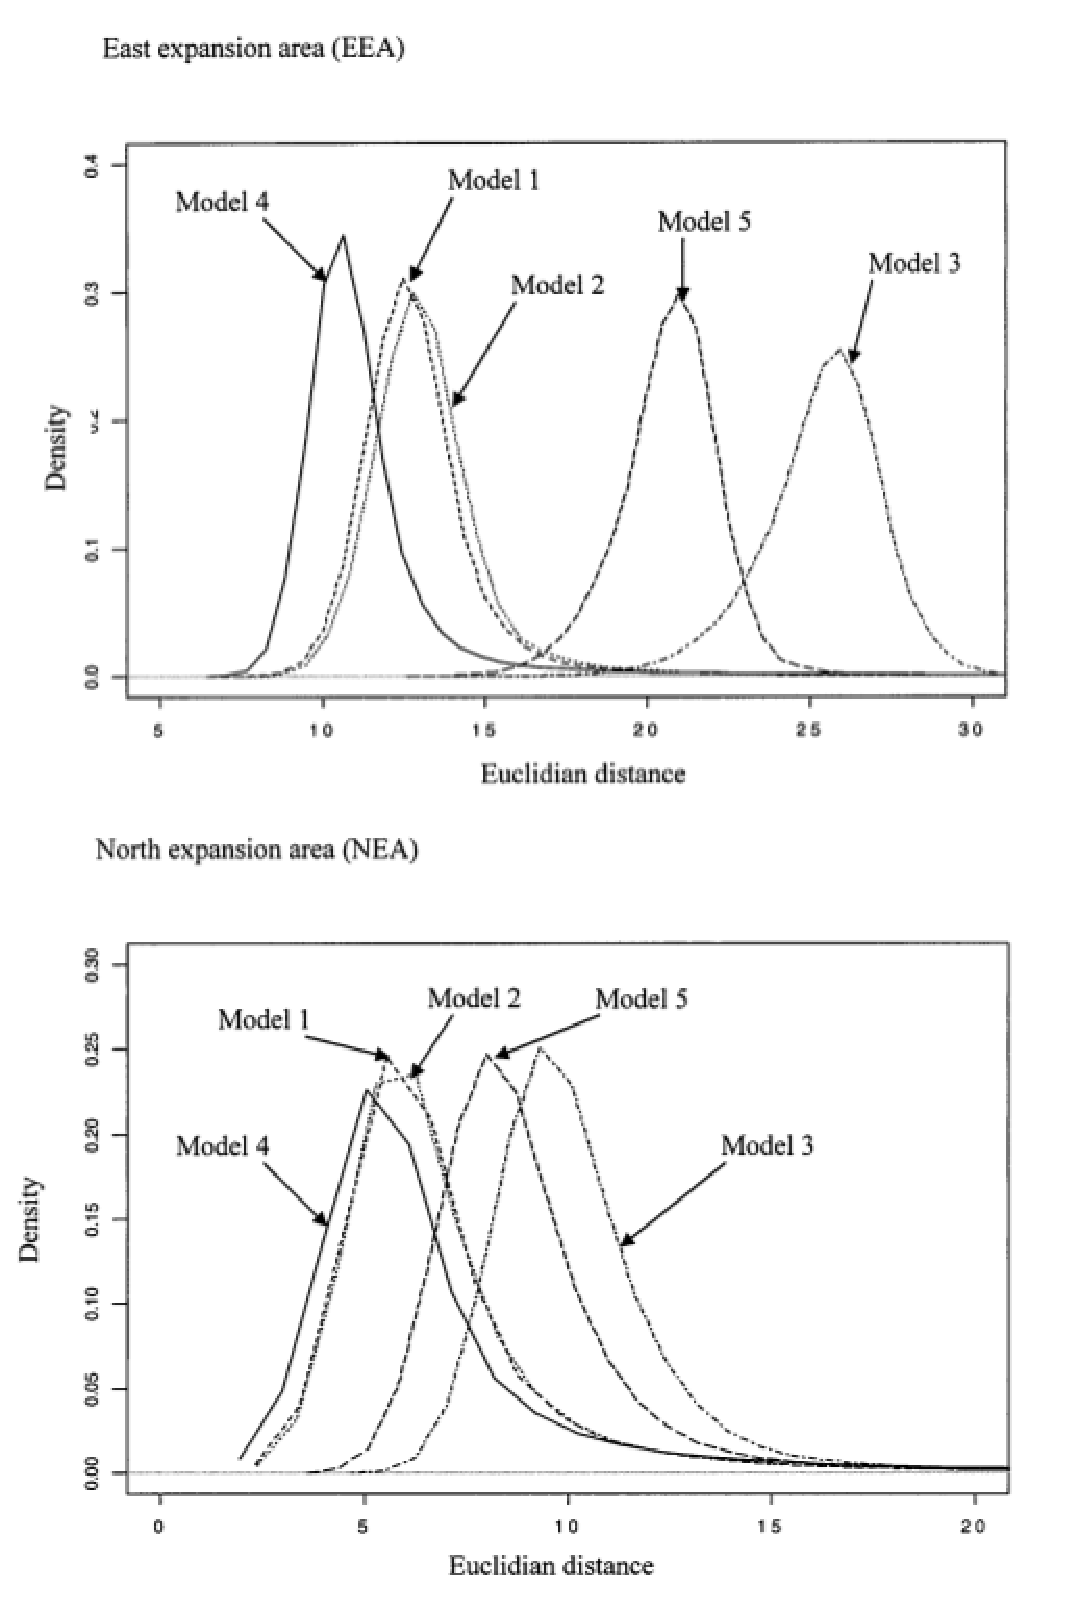
\includegraphics[width=4.5in]{cane-toad-models.eps}
\end{center}
\caption{Posterior distribution of $\delta$ for the five models
  considered in Estoup et al.~\cite{Estoup-etal-2004}.}\label{fig:cane-toad-models}
\end{figure}

Of course, we also have estimates for various parameters associated
with this model: 

\begin{itemize}

\item $N_{e_s}$: the effective population size when the population is
  stable.

\item $N_{e_f}$: the effective population size when a new population
  is founded.

\item $F_R$: the founding ratio, $N_{e_s}/N_{e_f}$.

\item $m$: the migration rate.

\item $N_{e_s}m$: the effective number of migrants per generation.

\end{itemize}

The estimates are summarized in Table~\ref{table:cane-toad}. Although
the credible intervals are fairly broad,\footnote{And notice that
  these are 90\% credible intervals, rather than the conventional 95\%
  credible intervals, which would be even broader.} there are a few
striking features that emerge from this analysis.

\begin{itemize}

\item Populations in the northern expansion area are larger, than
  those in the eastern expansion region. Estoup et
  al.~\cite{Estoup-etal-2004} suggest that this is consistent with
  other evidence suggesting that ecological conditions are more
  homogeneous in space and more favorable to cane toads in the north
  than in the east.

\item A smaller number of individuals is responsible for founding new
  populations in the east than in the north, and the ratio of
  ``equilibrium'' effective size to the size of the founding
  population is bigger in the east than in the north. (The second
  assertion is only weakly supported by the results.)

\item Migration among populations is more limited in the east than in
  the north. 

\end{itemize}

As Estoup et al.~\cite{Estoup-etal-2004} suggest, results like these
could be used to motivate and calibrate models designed to predict the
future course of the invasion, incorporating a balance between gene
flow (which can reduce local adaptation), natural selection, drift,
and colonization of new areas.

\begin{table}
\begin{center}
\begin{tabular}{ccr}
\hline\hline
Parameter & area & mean (5\%, 90\%) \\
\hline
$N_{e_s}$ & east & 744 (205, 1442) \\
         & north & 1685 (526, 2838) \\
$N_{e_f}$ & east & 78 (48, 118) \\
         & north & 311 (182, 448) \\
$F_R$    & east & 10.7 (2.4, 23.8) \\
         & north & 5.9 (1.6, 11.8) \\
$m$      & east & 0.014 ($6.0 \times 10^{-6}$, 0.064) \\
         & north & 0.117 ($1.4 \times 10^{-4}$, 0.664) \\
$N_{e_s}m$ & east & 4.7 (0.005, 19.9) \\
          & north & 188 (0.023, 883) \\
\hline
\end{tabular}
\end{center}
\caption{Posterior means and 90\% credible intervals for parameters of
  model 4 in the eastern and northern expansion areas of {\it Bufo
    marinus}.}\label{table:cane-toad}
\end{table}

\section*{Limitations of ABC}\index{Approximate Bayesian Computation!limitations}

If you've learned anything by now, you should have learned that there
is no perfect method. An obvious disadvantage of ABC relative to
either {\tt Migrate} or {\tt IMa2} is that it is much more
computationally intensive. 

\begin{itemize}

\item Because the scenarios that can be considered are much more
  complex, it simply takes a long time to simulate all of the data. 

\item In the last few years, one of the other disadvantages{\dash}that
  you had to know how to do some moderately complicated scripting to
  piece together several different packages in order to run
  analysis{\dash}has become less of a problem. {\tt popABC}
  (\url{http://code.google.com/p/popabc/} and {\tt DIYABC}
  (\url{http://www1.montpellier.inra.fr/CBGP/diyabc/}) make it {\it
    relatively\/} easy\footnote{Emphasis on ``relatively''.} to
  perform the simulations.

\item Selecting an appropriate set of summary statistics isn't easy,
  and it turns out that which set is most appropriate may depend on
  the value of the parameters that you're trying to estimate and the
  which of the scenarios that you're trying to compare is closest to
  the actual scenario applying to the populations from which you
  collected the data. Of course, if you knew what the parameter values
  were and which scenario was closest to the actual scenario, you
  wouldn't need to do ABC in the first place.

\item In the end, ABC allows you to compare a small number of
  evolutionary scenarios. It can tell you which of the scenarios
  you've imagined provides the best combination of fit to the data and
  parsimonious use of parameters (if you choose model comparison
  statistics that include both components), but it takes additional
  work to determine whether the model is adequate, in the sense that
  it does a good job of explaining the data. Moreover, even if you
  determine that the model is adequate, you can't exclude the
  possibility that there are other scenarios that might be equally
  adequate{\dash}or even better.

\end{itemize}


\chapter{Genetic structure of human populations in Great Britain}

As we've seen several times in this course, the amount of genetic data
available on humans is vastly greater than what is available for any
other organism. As a result, it's possible to use these data to gain
unusually deep insight into the recent history of many human
populations. Today's example comes from Great Britain, courtesy of a
very large consortium~\cite{Leslie-etal-2015}

\section*{Data}

\begin{itemize}

\item 2039 individuals with four grandparents born within 80km of one
  another, effectively studying alleles sampled from grandparents
  (ca. 1885). 

\item 6209 samples from 10 countries in continental Europe.

\item Autosomal SNPs genotyped in both samples~(ca. 500K). 

\end{itemize}

\section*{Results*}

Very little evidence of population structure within British sample

\begin{itemize}

\item Average pairwise $F_{ST}$: 0.0007

\item Maximum pairwise $F_{ST}$: 0.003

\end{itemize}

Individual assignment analysis of genotypes using {\tt
  fineSTRUCTURE}. Same principle as {\tt STRUCTURE}, but it models the
correlations among SNPs resulting from gametic disequilibrium, rather
than treating each locus as being independently inherited. The
analysis is on {\it haplotypes\/} rather than on alleles. In addition,
it clusters populations
hierarchically~(Figure~\ref{fig:fine-structure}\index{fineSTRUCTURE}\index{human
  population genetics}

\begin{figure}
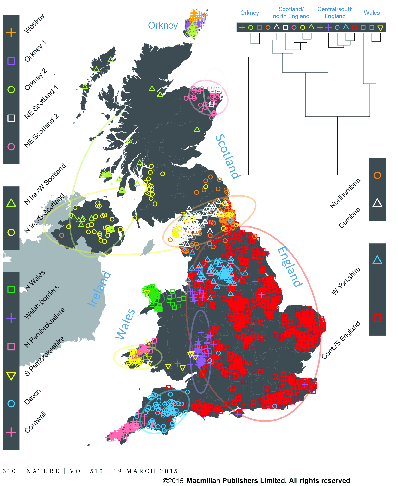
\includegraphics[height=0.9\textheight]{fine-structure-britain.eps}
\caption{{\tt fineSTRUCTURE} analysis of genotypes from Great Britain~(from~\cite{Leslie-etal-2015}).}
\end{figure}

Analysis of the European data identifies 52 groups. The authors used
{\tt Chromopainter} to construct each of the haplotypes detected in
their sample of 2039 individuals from the UK as a mosaic of haplotypes
derived from those found in their sample of 6209 individuals from
continental Europe. Since they know (a) the UK cluster to which each
UK individual belongs and (b) the European group from which each
individual contributing to the UK mosaic belongs they can estimate (c)
the proportion of ancestry for each UK cluster derived from each
European group. The results are shown in Figure~\ref{fig:UK-Europe}

\begin{figure}
\begin{center}
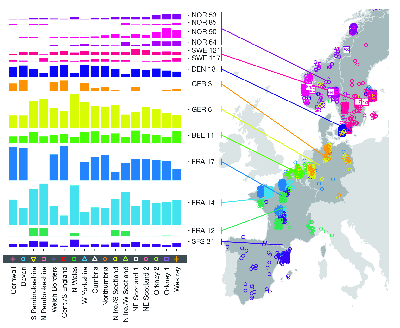
\includegraphics[width=0.9\textwidth]{UK-Europe.eps}
\end{center}
\caption{European ancestry of the 17 clusters identified in the UK~(from~\cite{Leslie-etal-2015}).}\label{fig:UK-Europe}
\end{figure}


\chapter{Two-locus population genetics}

So far in this course we've dealt only with variation at a single
locus. There are obviously many traits that are governed by more than
a single locus in whose evolution we might be interested. And for
those who are concerned with the use of genetic data for forensic
purposes, you'll know that forensic use of genetic data involves
genotype information from multiple loci. I won't be discussing
quantitative genetic variation for a few weeks, and I'm not going to
say anything about how population genetics gets applied to forensic
analyses, but I do want to introduce some basic principles of
multilocus population genetics that are relevant to our discussions of
the genetic structure of populations before moving on to the next
topic. To keep things relatively simple {\it multilocus\/} population
genetics will, for purposes of this lecture, mean {\it two-locus\/}
population genetics.

\section*{Gametic disequilibrium}

One of the most important properties of a two-locus system is that it
is no longer sufficient to talk about allele frequencies alone, even
in a population that satisfies all of the assumptions necessary for
genotypes to be in Hardy-Weinberg proportions at each locus. To see
why consider this. With two loci and two alleles there are four
possible gametes:\footnote{Think of drawing the Punnett square for a
dihybrid cross, if you want.}

\begin{center}
\begin{tabular}{lcccc}
Gamete    & $A_1B_1$ & $A_1B_2$ & $A_2B_1$ & $A_2B_2$ \\
Frequency & $x_{11}$ & $x_{12}$ & $x_{21}$ & $x_{22}$
\end{tabular}
\end{center}

If alleles are arranged randomly into gametes then,
\begin{eqnarray*}
x_{11} &=& p_1p_2 \\
x_{12} &=& p_1q_2 \\
x_{21} &=& q_1p_2 \\
x_{22} &=& q_1q_2 \quad ,
\end{eqnarray*}
where $p_1 = \hbox{freq}(A_1)$ and $p_2 = \hbox{freq}(A_2)$. But
alleles need not be arranged randomly into gametes. They may covary so
that when a gamete contains $A_1$ it is more likely to contain $B_1$
than a randomly chosen gamete, or they may covary so that a gamete
containing $A_1$ is less likely to contain $B_1$ than a randomly
chosen gamete. This covariance could be the result of the two loci
being in close physical association, but it doesn't have to
be. Whenever the alleles covary within gametes
\begin{eqnarray*}
x_{11} &=& p_1p_2 + D \\
x_{12} &=& p_1q_2 - D \\
x_{21} &=& q_1p_2 - D \\
x_{22} &=& q_1q_2 + D \quad ,
\end{eqnarray*}
where $D = x_{11}x_{22} - x_{12}x_{22}$ is known as the {\it gametic
  disequilibrium}.\footnote{You will sometimes see $D$ referred to as
  the linkage disequilibrium, but that's misleading. Alleles at
  different loci may be non-randomly associated even when they are not
  linked.} When $D \ne 0$ the alleles within gametes covary, and $D$
measures {\it statistical\/} association between them. It does not
(directly) measure the {\it physical\/} association. Similarly, $D =
0$ does not imply that the loci are unlinked, only that the alleles at
the two loci are arranged into gametes independently of one another.

\subsection*{A little diversion}

It probably isn't obvious why we can get away with only one $D$ for
all of the gamete frequencies. The short answer is:
\begin{quote}There are four gametes. That means we need three
  parameters to describe the four frequencies. $p_1$ and $p_2$ are
  two. $D$ is the third.
\end{quote}
Another way is to do a little algebra to verify that the definition is
self-consistent.
\begin{eqnarray*}
D &=& x_{11}x_{22} - x_{12}x_{21} \\
  &=& (p_1p_2 + D)(q_1q_2 + D) - (p_1q_2 - D)(q_1p_2 - D) \\
  &=& \left(p_1q_1p_2q_2 + D(p_1p_2 + q_1q_2) + D^2\right) \\
  && \quad - \left(p_1q_1p_2q_2 - D(p_1q_2 + q_1p_2) + D^2\right) \\
  &=& D(p_1p_2 + q_1q_2 + p_1q_2 + q_1p_2) \\
  &=& D\left(p_1(p_2 + q_2) + q_1(q_2 + p_2)\right) \\
  &=& D(p_1 + q_1) \\
  &=& D \quad. 
\end{eqnarray*}

\section*{Transmission genetics with two loci}

I'm going to construct a reduced version of a mating table to see how
gamete frequencies change from one generation to the next. There are
ten different two-locus genotypes (if we distinguish coupling,
$A_1B_1/A_2B_2$, from repulsion, $A_1B_2/A_2B_1$, heterozygotes as we
must for these purposes). So a full mating table would have 100
rows. If we assume all the conditions necessary for genotypes to be in
Hardy-Weinberg proportions apply, however, we can get away with just
calculating the frequency with which any one genotype will produce a
particular gamete.\footnote{We're assuming random union of {\it
    gametes\/} rather than random mating of {\it genotypes}.}

\begin{center}
\begin{tabular}{lccccc}
         &           & \multicolumn{4}{c}{Gametes} \\
Genotype & Frequency & $A_1B_1$ & $A_1B_2$ & $A_2B_1$ & $A_2B_2$ \\
\hline
$A_1B_1/A_1B_1$ & $x_{11}^2$ & 1 & 0 & 0 & 0 \\
$A_1B_1/A_1B_2$ & $2x_{11}x_{12}$ & $\half$ & $\half$ & 0 & 0 \\
$A_1B_1/A_2B_1$ & $2x_{11}x_{21}$ & $\half$ & 0 $\half$ & 0 \\
$A_1B_1/A_2B_2$ & $2x_{11}x_{22}$ & \oneminus & \rhalf & \rhalf & \oneminus \\
$A_1B_2/A_1B_2$ & $x_{12}^2$ & 0 & 1 & 0 & 0 \\
$A_1B_2/A_2B_1$ & $2x_{12}x_{21}$ & \rhalf & \oneminus & \oneminus & \rhalf \\
$A_1B_2/A_2B_2$ & $2x_{12}x_{22}$ & 0 & $\half$ & 0 & $\half$ \\
$A_2B_1/A_2B_1$ & $x_{21}^2$ & 0 & 0 & 1 & 0 \\
$A_2B_1/A_2B_2$ & $2x_{21}x_{22}$ & 0 & 0 & $\half$ & $\half$ \\
$A_2B_2/A_2B_2$ & $x_{22}^2$ & 0 & 0 & 0 & 1
\end{tabular}
\end{center}

\subsection*{Where do $\frac{1-r}{2}$ and $\frac{r}{2}$ come from?}

Consider the coupling double heterozygote, $A_1B_1/A_2B_2$. When
recombination doesn't happen, $A_1B_1$ and $A_2B_2$ occur in equal
frequency ($1/2$), and $A_1B_2$ and $A_2B_1$ don't occur at all. When
recombination happens, the four possible gametes occur in equal
frequency ($1/4$). So the recombination frequency,\footnote{The
frequency of recombinant gametes in double heterozygotes.} $r$, is
half the crossover frequency,\footnote{The frequency of cytological
crossover during meiosis.} $c$, i.e., $r = c/2$. Now the results of
crossing over can be expressed in this table:

\begin{center}
\begin{tabular}{c|cccc}
\hline\hline
Frequency & $A_1B_1$ & $A_1B_2$ & $A_2B_1$ & $A_2B_2$ \\
\hline
$1-c$     & $\half$  & 0        & 0        & $\half$ \\
$c$       & $\quarter$ & $\quarter$ & $\quarter$ & $\quarter$ \\
\hline
Total     & $\frac{2-c}{4}$ & $\frac{c}{4}$ & $\frac{c}{4}$
          & $\frac{2-c}{4}$ \\
          & $\frac{1-r}{2}$ & $\frac{r}{2}$ & $\frac{r}{2}$
          & $\frac{1-r}{2}$ \\          
\hline
\end{tabular}
\end{center}

\subsection*{Changes in gamete frequency}

We can use this table as we did earlier to calculate the frequency of
each gamete in the next generation. Specifically,
\begin{eqnarray*}
x_{11}' &=& x_{11}^2 + x_{11}x_{12} + x_{11}x_{21} + (1-r)x_{11}x_{22}
            + rx_{12}x_{21} \\
        &=& x_{11}(x_{11} + x_{12} + x_{21} + x_{22})
            - r(x_{11}x_{22} - x_{12}x_{21}) \\
        &=& x_{11} - rD \\
x_{12}' &=& x_{12} + rD \\
x_{21}' &=& x_{21} + rD \\
x_{22}' &=& x_{22} - rD \quad .
\end{eqnarray*}

\subsection*{No changes in allele frequency}

We can also calculate the frequencies of $A_1$ and $B_1$ after this
whole process:
\begin{eqnarray*}
p_1' &=& x_{11}' + x_{12}' \\
     &=& x_{11} - rD + x_{12} + rD \\
     &=& x_{11} + x_{12} \\
     &=& p_1 \\
p_2' &=& p_2 \quad .
\end{eqnarray*}
Since each locus is subject to all of the conditions necessary for
Hardy-Weinberg to apply at a single locus, allele frequencies don't
change at either locus. Furthermore, genotype frequencies at each
locus will be in Hardy-Weinberg proportions. But the two-locus gamete
frequencies change from one generation to the next.

\subsection*{Changes in $D$}

You can probably figure out that $D$ will eventually become zero, and
you can probably even guess that how quickly it becomes zero depends
on how frequent recombination is. But I'd be astonished if you could
guess exactly how rapidly $D$ decays as a function of $r$.  It takes a
little more algebra, but we can say precisely how rapid the decay will
be.
\begin{eqnarray*}
D' &=& x_{11}'x_{22}' - x_{12}'x_{21}' \\
   &=& (x_{11} - rD)(x_{22} - rD) - (x_{12} + rD)(x_{21} + rD) \\
   &=& x_{11}x_{22} - rD(x_{11} + x_{12}) + r^2D^2
       - (x_{12}x_{21} + rD(x_{12} + x_{21}) + r^2D^2) \\
   &=& x_{11}x_{22} - x_{12}x_{21} - rD(x_{11} + x_{12} + x_{21} + x_{22}) \\
   &=& D - rD \\
   &=& D(1-r)
\end{eqnarray*}
Notice that even if loci are unlinked, meaning that $r = 1/2$, $D$
does not reach 0 immediately. That state is reached only
asymptotically. The two-locus analogue of Hardy-Weinberg is that
gamete frequencies will {\it eventually\/} be equal to the product of
their constituent allele frequencies.

\section*{Population structure with two loci}

You can probably guess where this is going. With one locus I showed
you that there's a deficiency of heterozygotes in a combined sample
even if there's random mating within all populations of which the
sample is composed. The two-locus analog is that you can have gametic
disequilibrium in your combined sample even if the gametic
disequilibrium is zero in all of your constituent
populations. Table~\ref{table:d-structure} provides a simple numerical
example involving just two populations in which the combined sample
has equal proportions from each population.

\begin{table}
\begin{center}
\begin{tabular}{c|cccc|cc|c}
\hline\hline
           & \multicolumn{4}{c|}{Gamete frequencies} 
           & \multicolumn{2}{c|}{Allele frequencies} \\
Population & $A_1B_1$ & $A_1B_2$ & $A_2B_1$ & $A_2B_2$ 
           & $p_{i1}$ & $p_{i2}$ & $D$ \\
\hline
1          & 0.24     & 0.36     & 0.16    & 0.24
           & 0.60     & 0.40     & 0.00 \\
2          & 0.14     & 0.56     & 0.06    & 0.24
           & 0.70     & 0.20     & 0.00 \\
Combined   & 0.19     & 0.46     & 0.11    & 0.24
           & 0.65     & 0.30     & -0.005 \\
\hline
\end{tabular}
\end{center}
\caption{Gametic disequilibrium in a combined population
  sample.}\label{table:d-structure}
\end{table}

\subsection*{The gory details}

You knew that I wouldn't be satisfied with a numerical example, didn't
you? You knew there had to be some algebra coming, right? Well, here
it is. Let
\begin{eqnarray*}
D_i &=& x_{11,i} - p_{1i}p_{2i} \\
D_t &=& \bar x_{11} - \bar p_1\bar p_2 \quad ,
\end{eqnarray*}
where $\bar x_{11} = \frac{1}{K} \sum_{k=1}^K x_{11,k}$, $\bar p_1 =
\frac{1}{K} \sum_{k=1}^K p_{1k}$, and $\bar p_2 = \frac{1}{K}
\sum_{k=1}^K p_{2k}$. Given these definitions, we can now caclculate
$D_t$. 
\begin{eqnarray*}
D_t &=& \bar x_{11} - \bar p_1\bar p_2 \\
    &=& \frac{1}{K} \sum_{k=1}^K x_{11,k} - \bar p_1\bar p_2 \\
    &=& \frac{1}{K} \sum_{k=1}^K (p_{1k}p_{2k} + D_k) - \bar p_1\bar p_2 \\
    &=& \frac{1}{K} \sum_{k=1}^K (p_{1k}p_{2k} - \bar p_1\bar p_2) + \bar D \\
    &=& \mbox{Cov}(p_1, p_2) + \bar D \quad ,
\end{eqnarray*}
where $\mbox{Cov}(p_1, p_2)$ is the covariance in allele frequencies
across populations and $\bar D$ is the mean within-population gametic
disequilibrium. Suppose $D_i = 0$ for all subpopulations. Then $\bar D
= 0$, too (obviously). But that means that
\begin{eqnarray*}
D_t &=& \hbox{Cov}(p_1, p_2) \quad .
\end{eqnarray*}
So if allele frequencies covary across populations, i.e.,
$\mbox{Cov}(p_1, p_2) \ne 0$, then there will be non-random
association of alleles into gametes in the sample, i.e., $D_t \ne 0$,
even if there is random association alleles into gametes within each
population.\footnote{Well, duh! Covariation of allele frequencies
  across populations means that alleles are non-randomly associated
  across populations. What other result could you possibly expect?}

Returning to the example in Table~\ref{table:d-structure}
\begin{eqnarray*}
\mbox{Cov}(p_1, p_2) &=& 0.5(0.6-0.65)(0.4-0.3) + 0.5(0.7-0.65)(0.2-0.3) \\
                     &=& -0.005 \\
\bar x_{11}          &=& (0.65)(0.30) - 0.005 \\
                     &=& 0.19 \\
\bar x_{12}          &=& (0.65)(0.7) + 0.005 \\
                     &=& 0.46 \\
\bar x_{21}          &=& (0.35)(0.30) + 0.005 \\
                     &=& 0.11 \\
\bar x_{22}          &=& (0.35)(0.70) - 0.005 \\
                     &=& 0.24 \quad .
\end{eqnarray*}


\input{selection-components}
\documentclass[12pt]{article}
\usepackage{lecture}
\usepackage{html}
\usepackage{url}

\newcommand{\copyrightYears}{2001-2017}

\title{Selection at one locus with many alleles, fertility selection, and sexual selection} 

\begin{document}

\maketitle

\thispagestyle{first}

\section*{Introduction}

It's easy to extend the Hardy-Weinberg principle to multiple alleles
at a single locus. In fact, we already did this when we were
discussing the ABO blood group polymorphism. Just to get some notation
out of the way, though, let's define $x_{ij}$ as the frequency of
genotype $A_iA_j$ and $p_i$ as the frequency of allele
$A_i$. Then\index{Hardy-Weinberg proportions!multiple alleles}
\[
x_{ij} = \left\{
\begin{array}{ll}
p_i^2   & \mbox{if $i = j$} \\
2p_ip_j & \mbox{if $i \ne j$}
\end{array}
\right.
\]
Unfortunately, the simple principles we've learned for understanding
selection at one locus with two alleles don't generalize completely to
selection at one locus with many alleles~(or even three).

\begin{itemize}

\item For one locus with two alleles, heterozygote advantage
  guarantees maintenance of a polymorphism.

\item For one locus with multiple alleles, there are many different
  heterozygote genotypes. As a result, there is not a unique pattern
  identifiable as ``heterozygote advantage,'' and selection may
  eliminate one or more alleles at equilibrium even if all
  heterozygotes have a higher fitness than all homozygotes.

\end{itemize}

\section*{Selection at one locus with multiple alleles}

When we discussed selection at one locus with two alleles, I used the
following set of viabilities:

\begin{center}
\begin{tabular}{ccc}
$A_1A_1$ & $A_1A_2$ & $A_2A_2$ \\
$w_{11}$ & $w_{12}$ & $w_{22}$
\end{tabular}
\end{center}

\noindent You can probably guess where this is going. Namely, I'm
going to use $w_{ij}$ to denote the viability of genotype
$A_iA_j$. What you probably wouldn't thought of doing is writing it as
a matrix
\[
\begin{array}{ccc}
    & A_1  & A_2 \\
A_1 & w_{11} & w_{12} \\
A_2 & w_{12} & w_{22}
\end{array}
\]
Clearly we can extend an array like this to as many rows and columns
as we have alleles so that we can summarize any pattern of viability
selection with such a matrix. Notice that I didn't write both $w_{12}$
and $w_{21}$, because (normally) an individual's fitness doesn't
depend on whether it inherited a particular allele from its mom or its
dad.\footnote{If it's a locus that's subject to genomic imprinting, it
  may be necessary to distinguish $A_1A_2$ from $A_2A_1$. Isn't
  genetics fun?}

\subsection*{Marginal fitnesses and
  equilbria}\index{natural selection!multiple alleles, marginal viability}

After a little algebra it's possible to write down how allele
frequencies change in response to viability selection:\footnote{If
  you're ambitious (or a little weird), you might want to derive this
  yourself.}\index{selection!one locus, multiple alleles}
\[
p_i' = \frac{p_iw_i}{\bar w} \quad ,
\]
where $p_i = \sum_j p_i w_{ij}$ is the marginal fitness of allele $i$ and
$\bar w = \sum_i p_i^2 w_{ii} + \sum_i\sum_{j>i} 2p_ip_jw_{ij}$ is the
mean fitness in the population.\index{selection!marginal fitness}

It's easy to see\footnote{At least it's easy to see if you've stared a
  lot at these things in the past.} that if the marginal fitness of an
allele is less than the mean fitness of the population it will
decrease in frequency. If its marginal fitness is greater than the
mean fitness, it will increase in frequency.  If its marginal fitness
is equal to the mean fitness it won't change in frequency. So if
there's a stable polymorphism, all alleles present at that equilibrium
will have marginal fitnesses equal to the population mean
fitness. And, since they're all equal to the same thing, they're also
all equal to one another.

That's the only thing easy to say about selection with multiple
alleles. To say anything more complete would require a lot of linear
algebra. The only general conclusion I can mention, and I'll have to
leave it pretty vague, is that for a complete polymorphism\footnote{A
complete polymorphism is one in which all alleles are present.} to be
stable, none of the fitnesses can be too different from one
another. Let's play with an example to illustrate what I mean.

\section*{An example}\index{natural selection!sickle cell anemia}

The way we always teach about sickle-cell anemia isn't entirely
accurate. We talk as if there is a wild-type allele and the
sickle-cell allele. In fact, there are at least three alleles at this
locus in many populations where there is a high frequency of
sickle-cell anemia. In the wild-type, $A$, allele there is a glutamic
acid at position six of the $\beta$ chain of hemoglobin. In the most
common sickle-cell allele, $S$, there is a valine in this position. In
a rarer sickle-cell allele, $C$, there is a lysine in this
position. The fitness matrix looks like this:
\[
\begin{array}{cccc}
  & A     & S     & C \\
A & 0.976 & 1.138 & 1.103 \\
S &       & 0.192 & 0.407 \\
C &       &       & 0.550
\end{array}
\]
There is a stable, complete polymorphism with these allele
frequencies:\footnote{If you're wondering how I know that, feel free
  to ask. Otherwise, just take my word for it. Would I lie to you?
  (Don't answer that.)}
\begin{eqnarray*}
p_A &=& 0.83 \\
p_S &=& 0.07 \\
p_C &=& 0.10 \quad .
\end{eqnarray*}
If allele $C$ were absent, $A$ and $S$ would remain in a stable
polymorphism:
\begin{eqnarray*}
p_A &=& 0.85 \\
p_S &=& 0.15
\end{eqnarray*}
If allele $A$ were absent, however, the population would fix on allele
$C$.\footnote{Can you explain why? Take a close look at the fitnesses,
  and it should be fairly obvious.}

\begin{quote} {\bf Weird property \#1}: The existence of a stable,
  complete polymorphism does not imply that all subsets of alleles
  could exist in stable polymorphisms. Loss of one allele as a result
  of random chance could result in a cascading loss of
  diversity.\footnote{The same thing can happen in ecological
    commmunities. Loss of a single species from a stable community may
    lead to a cascading loss of several more.}
\end{quote}

\noindent If the fitness of $AS$ were 1.6 rather than 1.138, $C$ would
be lost from the population, although the $A-S$ polymorphism would
remain.

\begin{quote} {\bf Weird property \#2}: Increasing the selection in
  favor of a heterozygous genotype may cause selection to eliminate
  one or more of the alleles not in that heterozygous genotype. This
  also means that if a genotype with a very high fitness in
  heterozygous form is introduced into a population, the resulting
  selection may eliminate one or more of the alleles already present.
\end{quote}

\section*{Fertility selection}\index{natural selection!fertility selection}

So far we've been talking about natural selection that occurs as a
result of differences in the probability of survival, i.e., viability
selection. There are, of course, other ways in which natural selection
can occur:

\begin{itemize}

\item Heterozygotes may produce gametes in unequal frequencies, {\it
  segregation distortion}, or gametes may differ in their ability to
  participate in fertilization, {\it gametic selection}.\footnote{For
    the botanists in the room, I should point out that selection on
    the gametophyte stage of the life cycle (in plants with
    alternation of generations) is mathematically equivalent to
    gametic selection.}

\item Some genotypes may be more successful in finding mates than
  others, {\it sexual selection}.

\item The number of offspring produced by a mating may depend on
  maternal and paternal genotypes, {\it fertility selection}.

\end{itemize}

\noindent In fact, most studies that have measured components of
selection have identified far larger differences due to fertility than
to viability. Thus, fertility selection is a very important component
of natural selection in most populations of plants and animals. As
we'll see a little later, it turns out that sexual selection is
mathematically equivalent to a particular type of fertility
selection. But before we get to that, let's look carefully at the
mechanics of fertility selection.

\subsection*{Formulation of fertility selection}\index{natural selection!fertility selection, fertility matrix}

I introduced the idea of a fitness matrix earlier when we were
discussing selection at one locus with more than two alleles. Even if
we have only two alleles, it becomes useful to describe patterns of
fertility selection in terms of a fitness matrix. Describing the
matrix is easy. Writing it down gets messy. Each element in the table
is simply the average number of offspring produced by a given mated
pair. We write down the table with paternal genotypes in columns and
maternal genotypes in rows:
\begin{center}
\begin{tabular}{c|ccc}
\hline\hline
                  & \multicolumn{3}{c}{Paternal genotype} \\
Maternal genotype & $A_1A_1$ & $A_1A_2$ & $A_2A_2$ \\
\hline
$A_1A_1$ & $F_{11,11}$ & $F_{11,12}$ & $F_{11,22}$ \\
$A_1A_2$ & $F_{12,11}$ & $F_{12,12}$ & $F_{12,22}$ \\
$A_2A_2$ & $F_{22,11}$ & $F_{22,12}$ & $F_{22,22}$ \\
\hline
\end{tabular}
\end{center}
Then the frequency of genotype $A_1A_1$ after one generation of
fertility selection is:\footnote{I didn't say it, but you can probably
  guess that I'm assuming that all of the conditions for
  Hardy-Weinberg apply, except for the assumption that all matings
  leave the same number of offspring, on average.}
\begin{equation}
x_{11}' = \frac{x_{11}^2F_{11,11} + x_{11}x_{12}(F_{11,12} +
                F_{12,11})/2 + (x_{12}^2/4)F_{12,12}}{\bar F} \quad ,
\label{eq:fertility}
\end{equation}
where $\bar F$ is the mean fecundity of all matings in the
population.\footnote{As an exercise you might want to see if you can
derive the corresponding equations for $x_{12}'$ and $x_{22}'$.}

It probably won't surprise you to learn that it's very difficult to
say anything very general about how genotype frequenices will change
when there's fertility selection. Not only are there nine different
fitness parameters to worry about, but since genotypes are never
guaranteed to be in Hardy-Weinberg proportion, all of the algebra has
to be done on a system of three simultaneous equations.\footnote{And
you thought that dealing with one was bad enough!} There are three
weird properties that I'll mention:\index{natural selection!fertility selection, properties}

\begin{enumerate}

\item $\bar F'$ may be smaller than $\bar F$. Unlike selection on
viabilities in which fitness evolved to the maximum possible value,
there are situations in which fitness will evolve to the {\it
minimum\/} possible value when there's selection on
fertilities.\footnote{Fortunately, it takes rather weird fertility
schemes to produce such a result.}

\item A high fertility of heterozygote $\times$ heterozygote matings
is not sufficient to guarantee that the population will remain
polymorphic.

\item Selection may prevent loss of either allele, but there may be no
stable equilibria.

\end{enumerate}

\subsection*{Conditions for protected polymorphism}\index{natural selection!fertility selection, protected polymorphism}

There is one case in which it's fairly easy to understand the
consequences of selection, and that's when one of the two alleles is
very rare. Suppose, for example, that $A_1$ is very rare, then a
little algebraic trickery\footnote{The trickery isn't hard, just
tedious. Justifying the trickery is a little more involved, but not
too bad. If you're interested, drop by my office and I'll show you.}
shows that
\begin{eqnarray*}
x_{11}' &\approx& 0 \\
x_{12}' &\approx& \frac{x_{12}(F_{12,22} + F_{22,12})/2}{F_{22,22}}
\end{eqnarray*}
So $A_1$ will become more frequent if
\begin{equation}
(F_{12,22} + F_{22,12})/2 > F_{22,22} \label{eq:a-1}
\end{equation}
Similarly, $A_2$ will become more frequent when it's very rare when
\begin{equation}
(F_{11,12} + F_{12,11})/2 > F_{11,11} \label{eq:a-2} \quad .
\end{equation}
If both equation (\ref{eq:a-1}) and (\ref{eq:a-2}) are satisfied,
natural selection will tend to prevent either allele from being
eliminated. We have what's known as a {\it protected polymorphism}.

Conditions~(\ref{eq:a-1}) and~(\ref{eq:a-2}) are fairly easy to
interpret intuitively: There is a protected polymorphism if the
average fecundity of matings involving a heterozygote and the
``resident'' homozygote exceeds that of matings of the resident
homozygote with itself.\footnote{A ``resident'' homozygote is the one
  of which the populations is almost entirely composed when all but
  one allele is rare.}

{\bf NOTE:} It's entirely possible for neither inequality to be
satisfied {\it and\/} for their to be a stable polymorphism. In other
words, depending on where a population starts, selection may eliminate
one allele or the other or keep both segregating in the population in
a stable polymorphism.\footnote{Can you guess what pattern of
  fertilities is consistent with both a stable polymorphism and the
  {\it lack of\/} a protected polymorphism?}

\section*{Sexual selection}\index{natural selection!sexual selection}

A classic example of sexual selection is the peacock's ``tail''
feathers.\footnote{The brightly colored ``tail'' is actually the upper
  tail covert.} The long, elaborate feathers do nothing to promote
survival of male peacocks, but they are very important in determining
which males attract mates and which don't. If you'll recall, when we
originally derived the Hardy-Weinberg principle we said that the
matings occurred randomly. Sexual selection is clearly an instance of
non-random mating. Let's go back to our original mating table and see
how we need to modify it to accomodate sexual selection.

\begin{center}
\begin{tabular}{rcccc}
                       &           & \multicolumn{3}{c}{Offspring genotype} \\
Mating                 & Frequency     & $A_1A_1$ & $A_1A_2$ & $A_2A_2$ \\
\hline
$A_1A_1 \times A_1A_1$ & $x_{11}^fx_{11}^m$     &        1 &        0 &        0 \\
              $A_1A_2$ & $x_{11}^fx_{12}^m$ &    $\half$ &    $\half$ &        0 \\
              $A_2A_2$ & $x_{11}^fx_{22}^m$ &        0 &        1 &        0 \\
$A_1A_2 \times A_1A_1$ & $x_{12}^fx_{11}^m$ &    $\half$ &    $\half$ &        0 \\
              $A_1A_2$ & $x_{12}^fx_{12}^m$     &  $\fourth$ &    $\half$ &  $\fourth$ \\
              $A_1A_2$ & $x_{12}^fx_{22}^m$ &        0 &    $\half$ &    $\half$ \\
$A_2A_2 \times A_1A_1$ & $x_{22}^fx_{11}^m$ &        0 &        1 &        0 \\
              $A_1A_2$ & $x_{22}^fx_{12}^m$ &        0 &    $\half$ &    $\half$ \\
              $A_2A_2$ & $x_{22}^fx_{22}^m$     &        0 &
0 & 1 \\
\end{tabular}
\end{center}

What I've done is to assume that there is random mating in the
populations {\it among those individuals that are included in the
mating pool}. We'll assume that all females are mated so that
$x_{ij}^f = x_{ij}$.\footnote{There's a reason for doing this called
Bateman's principle that we can discuss, if you'd like.} We'll let the
relative attractiveness of the male genotypes be $a_{11}$, $a_{12}$,
and $a_{22}$. Then it's not too hard to convince yourself that
\begin{eqnarray*}
x_{11}^m &=& \frac{x_{11}a_{11}}{\bar a} \\
x_{12}^m &=& \frac{x_{12}a_{12}}{\bar a} \\
x_{22}^m &=& \frac{x_{22}a_{22}}{\bar a} \quad ,
\end{eqnarray*}
where $\bar a = x_{11}a_{11} + x_{12}a_{12} + x_{22}a_{22}$. A little
more algebra and you can see that
\begin{equation}
x_{11}' = \frac{x_{11}^2a_{11} + x_{11}x_{12}(a_{12} + a_{11})/2
                + x_{12}^2a_{12}/4}{\bar a} \label{eq:sexual}
\end{equation}
And we could derive similar equations for $x_{12}'$ and $x_{22}'$. Now
you're not likely to remember this, but equation~(\ref{eq:sexual})
bears a striking resemblance to one you saw earlier,
equation~(\ref{eq:fertility}). In fact, sexual selection is equivalent
to a particular type of fertility selection, in terms of how genotype
frequencies will change from one generation to the next. Specifically,
the fertility matrix corresponding to sexual selection on a male trait
is:
\[
\begin{array}{cccc}
       & A_1A_1 & A_1A_2 & A_2A_2 \\
A_1A_1 & a_{11} & a_{12} & a_{22} \\
A_1A_2 & a_{11} & a_{12} & a_{22} \\
A_2A_2 & a_{11} & a_{12} & a_{22}
\end{array}
\]

There are, of course, a couple of other things that make sexual
selection interesting. First, traits that are sexually selected in
males often come at a cost in viability, so there's a tradeoff between
survival and reproduction that can make the dynamics complicated and
interesting. Second, the evolution of a sexually selected trait
involves two traits: the male characteristic that is being selected
and a female preference for that trait. In fact the two tend to become
associated so that the female preference evokes a sexually selected
response in males, which evokes a stronger preference in females, and
so on and so on. This is a process Fisher referred to as ``runaway
sexual selection.''

\ccLicense

\end{document}

\chapter{Association mapping: BAMD}

We've now seen that a na{\"i}ve, locus-by-locus approach to
identifying associations between marker loci and SNPs could be
misleading, both because we have to correct for multiple
comparisons\footnote{Strictly speaking, we didn't see this in the
  context of association mapping, but we encountered it in our
  discussion of QTL mapping.} and, more importantly, because we need
to account for the possibility that loci are statistically associated
simply because there is genetic substructure within the
sample. Stephens and Balding~\cite{Stephens-Balding-2009} outline one
set of Bayesian approaches to dealing with both of these
problems. We'll focus on the problem of accounting for population
structure, using the approach implemented in {\tt BAMD}, an {\tt R}
package similar to {\tt R/qtl}.

\section*{The statistical model}\index{association mapping!linear mixed model}

{\tt BAMD}\footnote{And a couple of other packages we won't discuss,
  {\tt TASSEL} and {\tt EMMAX}.} uses a multiple regression approach
to investigate the relationship between genotypes at a marker locus
and phenotypes. Specifically, they use a ``mixed-model'' that allows
the residual variances and covariances to be specified in ways that
reflect the underlying population structure. Suppose $y_i$ is the
phenotype of the $i$th individual in our sample and
$\mbox{\boldmath$y$} = (y_1, \dots, y_I)$. Then the statistical model
is:\footnote{Hang on. This looks pretty complicated, but it's really
  not as bad as it looks.}
\[
\mbox{\boldmath$y$} = \mbox{\boldmath$X$}\beta +
\mbox{\boldmath$Z$}\gamma + \epsilon \quad ,
\]
where $\mbox{\boldmath$X$}$ is a matrix describing how each individual
is assigned to a particular genetic grouping,\footnote{For example,
  you could use {\tt STRUCTURE} to identify genetic groupings in your
  data. Then row $i$ of $\mbox{\boldmath$X$}$ would correspond to the
  posterior probability that individual $i$ is assigned to each of the
  groupings you identify.}, $\beta$ is a vector of coefficients
describing the mean phenotype associated with individuals belonging to
that grouping, $\mbox{\boldmath$Z$}$ is a matrix in which element $ij$
is the genotype of individual $i$ at locus $j$,\footnote{{\tt BAMD} is
  intended for the analysis of SNP data. Thus, the genotypes can be
  scored as 1, 2, or 3. Which homozygote is associated with genotype 1
  doesn't affect the results, only the sign of the associated
  coefficient.} $\gamma$ is a vector of coefficients describing the
effect of different genotypes at each locus,\footnote{These are the
  coefficients we're really interested in. They tell us the magnitude
  of the affect associated with a particular locus. In the
  implementation we're using, the relationship between genotype and
  phenotype is assumed to be strictly additive, since heterozygotes
  are perfectly intermediate.} and $\epsilon$ is a vector of
residuals.

In a typical regression problem, we'd assume $\epsilon \sim
\mbox{N}(0, \sigma^2\mbox{\boldmath$I$})$, where $\mbox{\boldmath$I$}$
is the identity matrix. Translating that to English,\footnote{Or at
  least translating it to something {\it closer\/} to English.} we'd
typically assume that the errors are independently distributed with a
mean of 0 and a variance of $\sigma^2$. In some applications, that's
not a good assumption. Some of the individuals included in the
analysis are related to one another. Fortunately, if you know (or can
estimate) that degree of relationship, {\tt BAMD} can help you out. If
$\mbox{\boldmath$R$}$ is a matrix in which element $ij$ indicates the
degree of relationship between individual $i$ and
$j$,\footnote{Individuals are perfectly related to themselves, so
  $r_{ii}=1$. Unrelated individuals have $r_{ij}=0$.}, then we
simply\footnote{It's simple because the authors of {\tt BAMD} included
  this possibility in their code. All you have to do is to specify
  $\mbox{\boldmath$R$}$. {\tt BAMD} will take care of the rest.} let
$\epsilon \sim \mbox{N}(0, \sigma^2\mbox{\boldmath$R$})$. Now we allow
the residual errors to be correlated when individuals are related and
to be uncorrelated when they are not.\index{association mapping!relatedness} 

There's only one more piece of the model that you need to understand
in order to interpret the output. If I tell you that {\tt BAMD} is an
acronym for {\bf B}ayesian {\bf A}ssociation with {\bf M}issing {\bf
  D}ata, you can probably guess that the last piece has something to
do with prior distributions. Here's what you need to know. We will,
obviously, have to place prior distributions on $\beta$, $\gamma$, and
$\sigma^2$. We don't need to talk much about the priors on $\beta$ or
$\sigma^2$. We simply assume $\beta_j \sim \mbox{uniform}$, and we use
a standard prior for variance paramters.\footnote{If you must know, we
  use $1/\sigma^2 \sim \mbox{G}(a, b)$, where $\mbox{G}$ stands for
  the Gamma distribution and $a$ and $b$ are its parameters.} The
prior for $\gamma$ is, however, a bit more
complicated.\index{association mapping!BAMD priors}

The covariates in $\mbox{\boldmath$X$}$ reflect aspects of the
experimental design, even if the elements of $\mbox{\boldmath$X$}$ are
inferred from a {\tt STRUCTURE} analysis.\footnote{Some people like to
  call these ``fixed'' effects.} They are, to some degree at least,
imposed by how we collected our samples of individuals. In contrast,
the covariates reflected in $\mbox{\boldmath$Z$}$ represent genotypes
selected at random from within those groups. Moreover, the set of
marker loci we chose isn't the only possible set we could have
chosen. As a result we have to think of both the genotypes we chose
and the coefficients associated with them as being samples from some
underlying distribution.\footnote{People who like to refer to
  $\mbox{\boldmath$X$}$ as fixed effects like to refer to these as
  ``random'' effects.} Specifically, we assume $\gamma_k \sim
\mbox{N}(0, \sigma^2\phi^2)$, where $\phi^2$ is simply a positive
constant that ``adjusts'' the variance of $\gamma_k$ relative to the
residual variance. Then we just put a standard prior on
$\phi^2$.\footnote{You may be able to guess, if you've been reading
  footnotes, that we use $1/\phi^2 \sim \mbox{G}(c,d)$.}

The good news is that once you've got your data into the right format,
{\tt BAMD} will take care of all of the calculations for you. It will
give you samples from the posterior distribution of $\beta$, $\gamma$,
$\sigma^2$, and $\phi^2$, from which you can derive the posterior
mean, the posterior standard deviation, and the credible
intervals.

\subsection*{What about the ``Missing Data'' part of the name?}

There's one more thing that {\tt BAMD} does for us behind the
scenes. In any real association analysis data set, every individual is
likely to be missing data at one or more loci. That's a problem. If
we're doing a multiple regression, we can't include sample points
where there are missing data, but if we dropped every individual for
which we couldn't score one or more SNPs, we wouldn't have any data
left. So what do we do? We ``impute'' the missing data, i.e., we use
the data we do have to guess what the data would have been if we'd
been able to observe it. {\tt BAMD} does this in a very sophisticated
and reliable way. As a result, we're able to include every individual
in our analysis and make use of all the data we've
collected.\footnote{If you're interested in why we can get away with
  what seems like making up data, stop by and talk to me. It involves
  a lot more statistics than I want to get into here.}


\chapter{The neutral theory of molecular evolution}

I didn't make a big deal of it in what we just went over, but in
deriving the Jukes-Cantor equation I used the phrase ``substitution
rate'' instead of the phrase ``mutation rate.'' As a preface to what
is about to follow, let me explain the difference.

\begin{itemize}

\item {\it Mutation rate\/} refers to the rate at which changes are
  incorporated into a nucleotide sequence during the process of
  replication, i.e., the probability that an allele differs from the
  copy of that in its parent from which it was derived. {\it Mutation
    rate\/} refers to the rate at which mutations
  arise.\index{mutation rate}

\item An allele substitution occurs when a newly arisen allele is
  incorporated into a population, e.g., when a newly arisen allele
  becomes fixed in a population. {\it Substitution rate\/} refers to
  the rate at which allele substitutions occur.\index{substitution rate} 

\end{itemize}

\noindent Mutation rates and substitution rates are obviously related
related{\dash}substitutions can't happen unless mutations occur, after
all{\dash}, but it's important to remember that they refer to
different processes.

\section*{Early empirical observations}

By the early 1960s amino acid sequences of hemoglobins and cytochrome
{\it c\/} for many mammals had been determined. When the sequences
were compared, investigators began to notice that the number of amino
acid differences between different pairs of mammals seemed to be
roughly proportional to the time since they had diverged from one
another, as inferred from the fossil record. Zuckerkandl and
Pauling~\cite{Zuckerkandl-Pauling65} proposed the {\it molecular clock
hypothesis\/} to explain these results. Specifically, they proposed
that there was a constant rate of amino acid substitution over
time. Sarich and Wilson~\cite{Sarich-Wilson67,Wilson-Sarich69} used
the molecular clock hypothesis to propose that humans and apes
diverged approximately 5 million years ago. While that proposal may
not seem particularly controversial now, it generated enormous
controversy at the time, because at the time many paleoanthropologists
interpreted the evidence to indicate humans diverged from apes as much
as 30 million years ago.\index{molecular clock}

One year after Zuckerkandl and Pauling's paper, Harris~\cite{Harris66}
and Hubby and Lewontin~\cite{Hubby-Lewontin66,Lewontin-Hubby66} showed
that protein electrophoresis could be used to reveal surprising
amounts of genetic variability within populations. Harris studied
10 loci in human populations, found three of them to be polymorphic,
and identified one locus with three alleles. Hubby and Lewontin
studied 18 loci in {\it Drosophila pseudoobscura\/}, found seven to be
polymorphic, and five that had three or more alleles.

Both sets of observations posed real challenges for evolutionary
geneticists. It was difficult to imagine an evolutionary mechanism
that could produce a constant rate of substitution. It was similarly
difficult to imagine that natural selection could maintain so much
polymorphism within populations. The ``cost of selection,'' as Haldane
called it would simply be too high.

\section*{Neutral substitutions and neutral variation}

Kimura~\cite{Kimura68} and King and Jukes~\cite{King-Jukes69} proposed
a way to solve both empirical problems. If the vast majority of amino
acid substitutions are selectively neutral, then substitutions will
occur at approximately a constant rate~(assuming that mutation rates
don't vary over time) and it will be easy to maintain lots of
polymorphism within populations because there will be no cost of
selection. I'll develop both of those points in a bit more detail in
just a moment, but let me first be precise about what the neutral
theory of molecular evolution actually proposes. More specifically,
let me first be precise about what it does {\it not\/} propose. I'll
do so specifically in the context of protein evolution for now,
although we'll broaden the scope later.

\begin{itemize}

\item {\it The neutral theory asserts that alternative alleles at
    variable protein loci are selectively neutral.} This does {\it
    not\/} mean that the locus is unimportant, only that the
  alternative alleles found at this locus are selectively
  neutral.\index{neutral alleles}

\begin{itemize}

\item Glucose-phosphate isomerase is an esssential enzyme. It
  catalyzes the first step of glycolysis, the conversion of
  glucose-6-phosphate into fructose-6-phosphate. 

\item Natural populations of many, perhaps most, populations of plants
  and animals are polymorphic at this locus, i.e., they have two or
  more alleles with different amino acid sequences.

\item The neutral theory asserts that the alternative alleles are
  selectively neutral.

\end{itemize}

\item By {\it selectively neutral\/} we do {\it not\/} mean that the
  alternative alleles have no effect on physiology or fitness. We mean
  that the selection among different genotypes at this locus is
  sufficiently weak that the pattern of variation is determined by the
  interaction of mutation, drift, mating system, and migration. This
  is roughly equivalent to saying that $N_es < 1$, where $N_e$ is the
  effective population size and $s$ is the selection coefficient on
  alleles at this locus.

\begin{itemize}

\item Experiments in {\it Colias\/} butterflies, and other organisms
  have shown that different electrophoretic variants of GPI have
  different enzymatic capabilities and different thermal
  stabilities. In some cases, these differences have been related to
  differences in individual performance.

\item If populations of {\it Colias\/} are large and the differences
  in fitness associated with differences in genotype are large, i.e.,
  if $N_es > 1$, then selection plays a predominant role in
  determining patterns of diversity at this locus, i.e., the neutral
  theory of molecular evolution would not apply.

\item If populations of {\it Colias\/} are small or the differences in
  fitness associated with differences in genotype are small, or both,
  then drift plays a predominant role in determining patterns of
  diversity at this locus, i.e., the neutral theory of molecular
  evolution applies.

\end{itemize}

\end{itemize}

\noindent In short, the neutral theory of molecular really asserts
only that observed amino acid substitutions and polymorphisms are {\it
effectively\/} neutral, not that the loci involved are unimportant or
that allelic differences at those loci have no effect on
fitness.\index{neutral theory!effective neutrality}\index{effective neutrality}

\subsection*{The rate of molecular evolution}

We're now going to calculate the rate of molecular evolution, i.e.,
the rate of allelic substitution, under the hypothesis that mutations
are selectively neutral. To get that rate we need two things: the rate
at which new mutations occur and the probability with which new
mutations are fixed. In a word equation\index{molecular clock!derivation}
\begin{eqnarray*}
\mbox{\# of substitutions/generation} &=& (\mbox{\# of mutations/generation})\times(\mbox{probability
  of fixation}) \\
\lambda &=& \mu_0p_0 \quad .
\end{eqnarray*}
Surprisingly,\footnote{Or perhaps not.} it's pretty easy to calculate
both $\mu_0$ and $p_0$ from first principles.

In a diploid population of size $N$, there are $2N$ gametes. The
probability that any one of them mutates is just the mutation rate,
$\mu$, so
\begin{equation}
\mu_0 = 2N\mu \quad . \label{eq:mu-0}
\end{equation}
To calculate the probability of fixation, we have to say something
about the dynamics of alleles in populations. Let's suppose that we're
dealing with a single population, to keep things simple. Now, you have
to remember a little of what you learned about the properties of
genetic drift. If the current frequency of an allele is $p_0$, what's
the probability that is eventually fixed?  $p_0$. When a new mutation
occurs there's only one copy of it,\footnote{By definition. It's new.}
so the frequency of a newly arisen mutation is $1/2N$ and
\begin{equation}
p_0 = \frac{1}{2N} \quad . \label{eq:p-0}
\end{equation}
Putting~(\ref{eq:mu-0}) and~(\ref{eq:p-0}) together we find
\begin{eqnarray*}
\lambda &=& \mu_0p_0 \\
        &=& (2N\mu)\left(\frac{1}{2N}\right) \\
        &=& \mu \quad .
\end{eqnarray*}
In other words, if mutations are selectively neutral, the substitution
rate is equal to the mutation rate. Since mutation rates are (mostly)
governed by physical factors that remain relatively constant, mutation
rates should remain constant, implying that substitution rates should
remain constant if substitutions are selectively neutral. In short, if
mutations are selectively neutral, we expect a molecular clock.

\subsection*{Diversity in populations}

Protein-coding genes consist of hundreds or thousands of nucleotides,
each of which could mutate to one of three other
nucleotides.\footnote{Why three when there are four nucleotides?
  Because if the nucleotide at a certain position is an A, for
  example, it can only {\it change\/} to a C, G, or T.} That's not an
infinite number of possibilities, but it's pretty large.\footnote{If a
  protein consists of 400 amino acids, that's 1200 nucleotides. There
  are $4^{1200} \approx 10^{720}$ different sequences that are 1200
  nucleotides long.} It suggests that we could treat every mutation
that occurs as if it were completely new, a mutation that has never
been seen before and will never be seen again. Does that description
ring any bells? Does the infinite alleles model sound familiar? It
should, because it exactly fits the situation I've just
described.\index{mutation!infinite alleles model}

Having remembered that this situation is well described by the
infinite alleles model, I'm sure you'll also remember that we can
calculate the equilibrium inbreeding coefficient for the infinite
alleles model, i.e.,
\[
f = \frac{1}{4N_e\mu + 1} \quad .
\]
What's important about this for our purposes, is that to the extent
that the infinite alleles model is appropriate for molecular data,
then $f$ is the frequency of homozygotes we should see in populations
and $1-f$ is the frequency of heterozygotes. So in large populations
we should find more diversity than in small ones, which is roughly
what we do find. Notice, however, that here we're talking about
heterozygosity at individual nucleotide positions,\footnote{Since the
  mutation rate we're talking about applies to individual nucleotide
  positions.} not heterozygosity of halpotypes.

\section*{Conclusions}

In broad outline then, the neutral theory does a pretty good job of
dealing with at least some types of molecular data. I'm sure that some
of you are already thinking, ``But what about third codon positions
{\it versus\/} first and second?'' or ``What about the observation
that histone loci evolve much more slowly than interferons or MHC
loci?''  Those are good questions, and those are where we're going
next. As we'll see, molecular evolutionists have elaborated the
framework extensively\footnote{That mean's they've made it more
  complicated.} in the last thirty years, but these basic principles
underlie every investigation that's conducted. That's why I wanted to
spend a fair amount of time going over the logic and
consequences. Besides, it's a rare case in population genetics where
the fundamental mathematics that lies behind some important
predictions are easy to understand.\footnote{It's the concepts that
  get tricky, not the algebra, or at least that's what I think.}


\chapter{Evolution in multigene families}

We now know a lot about the dynamics of nucleotide substitutions
within existing genes, but we've neglected one key component of
molecular evolution. We haven't talked about where new genes come
from. It's important to understand this phenomenon because, after all,
new metabolic functions are likely to arise only when there are new
genes that can perform them. It's not likely that an existing gene can
adopt a new function while continuing to serve its old one.

Fundamentally the source of new genes is the {\it duplication\/} of
existing genes and their {\it divergence\/} in function. As we'll see
in a moment, for example, genes coding for myogblobin and hemoglobin
in mammals are descendants of a single common ancestor. That's the
duplication. Myoglobin is involved in oxygen metabolism in muscle,
while hemoglobin is involved in oxygen transport in blood. That's the
divergence. Although there are many interesting things to say about
the processes by which duplication and divergence occur, we're going
to focus on the pattern of nucleotide sequence evolution that arises
as a result.

\section*{Globin evolution}\index{globins}

I've just pointed out the distinction between myoglobin and
hemoglobin. You may also remember that hemoglobin is a multimeric
protein consisting of four subunits, 2 $\alpha$ subunits and 2 $\beta$
subunits. What you may not know is that in humans there are actually
two types of $\alpha$ hemoglobin and four types of $\beta$ hemoglobin,
each coded by a different genetic locus~(see
Table~\ref{table:globins}). The five $\alpha$-globin loci ($\alpha_1$,
$\alpha_2$, $\zeta$, and two non-functional pseudogenes) are found in a
cluster on chromosome 16. The six $\beta$-globin loci ($\epsilon$,
$\gamma_G$, $\gamma_A$, $\delta$, $\beta$, and a pseudogene) are found
in a cluster on chromosome 11. The myoglobin locus is on chromosome
22.

\begin{table}
\begin{center}
\begin{tabular}{l|cc}
\hline\hline
Developmental stage & $\alpha$ globin & $\beta$ globin \\
\hline
Embryo & $\zeta$  & $\epsilon$ \\
       & $\alpha$ & $\epsilon$ \\
Fetus  & $\alpha$ & $\beta$ \\
       & $\alpha$  & $\gamma$ \\
Adult  & $\alpha$ & $\beta$ \\
       & $\alpha$ & $\delta$ \\
\hline
\end{tabular}
\end{center}
\caption{Human hemoglobins arranged in developmental sequence. Adult
  hemoglobins composed of 2$\alpha$ and 2$\delta$ subunits typically
  account for less than 3\% of hemoglobins in adults (\myurl{http://sickle.bwh.harvard.edu/hbsynthesis.html}).}\label{table:globins}
\end{table}

Not only do we have all of these different types of globin genes in
our bodies, they're all related to one another. Comparative sequence
analysis has shown that vertebrate myoglobin and hemoglobins diverged
from one another about 450 million years ago. Figure~\ref{fig:globins}
shows a phylogenetic analysis of part of the globin gene family,
namely the $\beta$ globin genes within tetrapods. If you stare at this
tree for a while, you'll notice a couple of interesting things:

\begin{itemize}

\item Eutherian $\beta$ and $\delta$ globins are more closely related
  to marsupial $\beta$ globins than they are to eutherian $\epsilon$
  or $\gamma$ globins.

\item Marsupial $\beta$ globin is more closely related to eutherian
  $\beta$ and $\delta$ globins than it is to marsupial $\epsilon$
  globin. 

\end{itemize}

\begin{figure}
\begin{center}
\resizebox{0.9\textwidth}{!}{\includegraphics{globin-gene-tree.eps}}
\end{center}
\caption{Evolution of $\beta$-globin genes in tetrapods drawn as a
  gene tree~(from~\cite{Opazo-etal-2008}).}\label{fig:globins}
\end{figure}

\noindent To put that another way, $\beta$ globin genes within humans
(a eutherian) are more closely related to $\beta$ globin genes in
kangaroos (a marsupial) than to $\epsilon$ globin genes in
humans. Strange as it seems, this pattern is exactly what we expect as
a result of duplication and divergence. 

Up to the time that a gene becomes duplicated, its evolutionary
history matches the evolutionary history of the organisms containing
it.  Once there are duplicate copies, each follows an independent
evolutionary history. Each traces the history of speciation and
divergence. And over long periods duplicate copies of the same gene
share more recent common ancestry with copies of the same gene in a
different species than they do with duplicate genes in the same
genome. You can see that in this example if we redraw the gene tree in
Figure~ref{fig:globins} as a species tree with the gene tree inside
it~(Figure~\ref{fig:globins-species}). 

\begin{figure}
\begin{center}
\resizebox{0.9\textwidth}{!}{\includegraphics{globin-species-tree.eps}}
\end{center}
\caption{Evolution of $\beta$-globin genes in tetrapods drawn as a
  species tree~(from~\cite{Opazo-etal-2008}).}\label{fig:globins-species}
\end{figure}

A history of duplication and divergence in multigene families makes it
important to distinguish between two classes of related loci: those
that represent the same locus in different species and between which
divergence is a result of species divergence are {\it
  orthologs}.\index{ortholog}\index{multigene family!ortholog} Those
that represent different loci and between which divergence occurred
after duplication of an ancestral gene are {\it
  paralogs}.\index{paralog}\index{multigene family!paralog} The
$\beta$-globin loci of humans and chickens are orthologous. The
$\alpha$- and $\beta$-globin loci of any pair of taxa are paralogous.

As multigene families go, the globin family is relatively simple and
easy to understand. There are only about a dozen loci involved, one
isolated locus (myoglobin) and two clusters of loci ($\alpha$- and
$\beta$-globins). You'll find a diagram of the $\beta$-globin cluster
in Figure~\ref{fig:beta-globin}. As you can see the $\beta$-globins
are not only evolutionarily related to one another they occur
relatively close to one another on chromosome 11 in humans.

\begin{figure}
\begin{center}
\includegraphics[angle=270,scale=0.5]{beta-globin.eps}
\caption{Structure of the human $\beta$-globin gene cluster. \%
  identity refers to similarity to the mouse $\beta$-globin
  sequence. From
  \myurl{http://globin.cse.psu.edu/html/pip/betaglobin/iplot.ps}
  (retrieved 28 Nov 2006).}\label{fig:beta-globin}
\end{center}
\end{figure}

Other families are far more complex. Class I and class II MHC loci,
for example are part of the same multigene family. Moreover,
immunoglobulins, T-cell receptors, and, and MHC loci are part of a
larger superfamily of genes, i.e., all are ultimately derived from a
common ancestral gene by duplication and
divergence. Table~\ref{table:superfamilies} lists a few examples of
multigene families and superfamilies in the human genome and the
number of proteins produced.\index{multigene family!examples}

\begin{table}
\begin{center}
\begin{tabular}{ll}
\hline\hline
Protein family domain & Number of proteins \\
\hline
Actin                 & 61 \\
Immunoglobulin        & 381 \\
Fibronectin type I    & 5 \\
Fibronectin type II   & 11 \\
Fibronectin type III  & 106 \\
Histone \\
\quad H2A/H2B/H3/H4   & 75 \\
Homeobox              & 160 \\
Immunoglobulin        & 381 \\
MHC Class I           & 18 \\
MHC Class II$\alpha$  & 5 \\
MHC Class II$\beta$   & 7 \\
T-cell receptor $\alpha$ & 16 \\
T-cell receptor $\beta$  & 15 \\
T-cell receptor $\gamma$ & 1 \\
T-cell receptor $\delta$ & 1 \\
Zinc finger, C2H2     & 564 \\
Zinc finger, C3HC4    & 135 \\
\hline
\end{tabular}
\end{center}
\caption{A few gene families from the human genome~(adapted from~\cite{Ohta2003,Venter-etal2001}).}\label{table:superfamilies}
\end{table}

\section*{Concerted evolution}\index{concerted evolution}
\index{multigene family!concerted evolution}

Although the patterns of gene relationships produced through
duplication and divergence can be quite complex, the processes are
relatively easy to understand. In some multigene families, however,
something quite different seems to be going on. In many plants and
animals, genes encoding ribosomal RNAs are present in hundreds of
copies and arranged end to end in long tandem arrays in one or a few
places in the genome~(Figure~\ref{fig:rdna}). Brown et
al.~\cite{Brown-etal72} compared the ribosomal RNA of {\it Xenopus
  laevis\/} and {\it X. mulleri\/} and found a surprising
pattern. There was little or no detectable variation among copies of
the repeat units within either species, in spite of substantial
divergence between them. This pattern can't be explained by purifying
selection. Members of the gene family presumably diverged before {\it
  X. laevis\/} and {\it X. mulleri\/} diverged. Thus, we would expect
more divergence among copies {\it within\/} species than {\it
  between\/} species, i.e., the pattern we see in the globin
family. Explaining this pattern requires some mechanism that causes
different copies of the repeat to be homogenized within each species
while allowing the repeats to diverge between species. The phenomenon
is referred to as concerted evolution.

\begin{figure}
\begin{center}
\resizebox{0.75\textwidth}{!}{\includegraphics{rdna.eps}}
\end{center}
\caption{Diagrammatic representation of ribosomal DNA in vascular
  plant genomes~(from Muir \& Schl{\"o}tterer, 1999
  \myurl{http://webdoc.sub.gwdg.de/ebook/y/1999/whichmarker/m11/Chap11.htm}).}\label{fig:rdna}
\end{figure}

Two mechanisms that can result in concerted evolution have been widely
studied: unequal crossing over and gene conversion.  \index{multigene
  family!unequal crossing over} \index{multigene family!gene
  conversion} \index{unequal crossing over} \index{gene conversion}
Both depend on misalignments during meiotic prophase. These
misalignments allow a mutation that occurs in one copy of a tandemly
repeated gene array to ``spread'' to other copies of the gene
array. Tomoko Ohta and Thomas Nagylaki have provided exhaustive
mathematical treatments of the process~\cite{Nagylaki84,Ohta84}. We'll
follow Ohta's treatment, but keep it fairly simple and
straightforward. First some notation:\footnote{See
Figure~\ref{fig:ohta-multigene} for a diagram that you may find
helpful}
\begin{eqnarray*}
f   &=& \mbox{P}(\mbox{two alleles at same locus are ibd}) \\
c_1 &=& \mbox{P}(\mbox{two alleles at different loci in same
  chromosome are ibd}) \\
c_2 &=& \mbox{P}(\mbox{two alleles at different loci in different
  chromosomes are ibd}) \\
\mu &=& \mbox{mutation rate} \\
n &=& \mbox{no.\ of loci in family} \\
\lambda &=& \mbox{rate of gene conversion}
\end{eqnarray*}

\begin{figure}
\resizebox{\textwidth}{!}{\includegraphics{ohta-multigene.eps}}
\caption{Types of identity by descent within a tandem
  repeat~(from~\cite{Ohta-1982}).}\label{fig:ohta-multigene}
\end{figure}

Now remember that for the infinite alleles model
\[
f = \frac{1}{4N_e\mu + 1} \quad , \\
\]
and $f$ is the probability that neither allele has undergone
mutation. By analogy
\[
g = \frac{1}{4N_e\lambda + 1} \quad , \\
\]
where $g$ is the probability that two alleles at a homologous position
are ibd in the sense that neither has ever moved from that position in
the array. Thus, for our model
\begin{eqnarray*}
f &=& P(\mbox{neither has moved})\mbox{P}(\mbox{ibd}) \\
  && + \mbox{P}(\mbox{one has moved})\mbox{P}(\mbox{ibd anyway}) \\
  &=&
  \left(\frac{1}{4N_e\lambda+1}\right)\left(\frac{1}{4N_e\mu+1}\right) 
  + \left(\frac{4N_e\lambda}{4N_e\lambda+1}\right)c_2 \\
  &\approx& \frac{4N_e\lambda c_2 + 1}{4N_e\lambda + 4N_e\mu + 1}
  \\
c_1 = c_2 &=& \frac{\lambda}{\lambda + (n-1)\mu} \quad .
\end{eqnarray*}

Notice that $(n-1)\mu$ is approximately the number of mutations that
occur in a single array every generation. Consider two possibilities:

\begin{itemize}

\item {\it Gene conversion occurs much more often than mutation\/}:
  $\lambda \gg (n-1)\mu$.

Under these conditions $c_2 \approx 1$ and $f \approx 1$. In short,
all copies of alleles at every locus in the array are virtually
identical{\dash}concerted evolution.

\item {\it Gene conversion occurs much less often than mutation\/}:
  $\lambda \ll (n-1)\mu$.

Under these conditions $c_2 \approx 0$ and $f \approx \frac{1}{4N_e\mu
  + 1}$. In short, copies of alleles at different loci are almost
  certain to be different from one another, and the diversity at any
  single locus matches neutral expectations{\dash}non-concerted
  evolution.

\end{itemize}


\chapter{Patterns of selection on nucleotide polymorphisms}

We've now seen one good example of natural selection acting to
maintain diversity at the molecular level, but that example involves
only a pair of alleles. Let's examine how selection operates on a more
complex polymorphism involving many alleles and several loci,
specifically the polymorphsims at the major histocompatibility complex
(MHC) loci of vertebrates.

MHC molecules are responsible for cellular immune responses in
vertebrates. They are expressed on all nucleated cells in vertebrates,
and they present intracellularly processed ``foreign'' antigens to T
cell receptor lymphocytes. When the MHC $+$ antigen complex is
recognized, a cytotoxic reaction is triggered killing cells presenting
the antigen. It's been known for many years that the genes are highly
polymorphic.\footnote{They were discovered as a result of
  investigations into rejection of transplanted organs and
  tissues. They are the loci governing acceptance/rejection of
  transplants in vertebrates.} Although plausible adaptive scenarios
for that variation existed, a competing hypothesis had been that MHC
loci were ``hypervariable'' not because of selection for diversity,
but because of an unusually high mutation rate.

\section*{Patterns of amino acid substitution at MHC loci}\index{MHC polymorphism}

Hughes and Nei~\cite{Hughes-Nei88} recognized that these hypotheses
could be distinguished by comparing rates of synonymous and
non-synonymous substitution at MHC loci. The results are summarized
in Table~\ref{table:hughes-nei}. Notice that they distinguished among
three functional regions within the protein and calculated statistics
separately for each one:

\begin{itemize}

\item codons in the {\it antigen recognition site},

\item the remaining codons in the extracellular domain involved in
  presenting the antigen on the cell surface~(the $\alpha_1$ and
  $\alpha_2$ domains), and

\item codons in the extracellular domain that are not directly
  involved in presenting the antigen on the cell surface~(the
  $\alpha_3$ domain).

\end{itemize}
Hughes and Nei argue that the unusually low value of $K_s$ in the
$\alpha_3$ domain of H2-L in mice is due to interlocus genetic
exchange. If we discount that set of data as unreliable, a clear
pattern emerges.

\begin{table}
\begin{center}
\begin{tabular}{lcccccc}
\hline\hline
      & \multicolumn{2}{c}{ARS} 
      & \multicolumn{2}{c}{$\alpha_1$ and $\alpha_2$}
      & \multicolumn{2}{c}{$\alpha_3$} \\
Locus & $K_s$ & $K_a$ & $K_s$ & $K_a$ & $K_s$ & $K_a$ \\
\hline
Human \\
\quad HLA-A & 3.5 & 13.3*** &  2.5 & 1.6 & 9.5 & 1.6** \\
\quad HLA-B & 7.1 & 18.1**  &  6.9 & 2.4 & 1.5 & 0.5 \\
\quad HLA-C & 3.8 &  8.8    & 10.4 & 4.8 & 2.1 & 1.0 \\
Mean        & 4.7 & 14.1*** &  5.1 & 2.4 & 5.8 & 1.1** \\
\\
Mouse \\
\quad H2-K  & 15.0 & 22.9   &  8.7 & 5.8 & 2.3 & 4.0 \\
\quad H2-L  & 11.4 & 19.5   &  8.8 & 6.8 & 0.0 & 2.5** \\
Mean        & 13.2 & 21.2*  &  8.8 & 6.3 & 1.2 & 3.6** \\
\hline
\end{tabular}
\end{center}
\caption{Rates of synonymous and non-synonymous substitution for loci
  in the MHC complex of humans and mice~(modified from~\cite{Li97} and
  based on~\cite{Hughes-Nei88}). ARS refers to the antigen recognition
  site. Significant differences between $K_s$ and $K_a$ are denoted
  as: * ($P < 0.05$), ** ($P < 0.01$), and *** ($P <
  0.001$).}\label{table:hughes-nei}
\end{table}\index{MHC!synonymous and non-synonymous substitutions}

\begin{itemize}

\item In the part of the MHC molecule that is not directly involved in
  presenting antigen, $\alpha_3$ in humans, the rate of non-synonymous
  substitution is significantly lower than the rate of synonymous
  substitution, i.e., there is selection {\it against\/} amino acid
  substitutions.\footnote{No surprise there. That's the ``sledgehammer
    principle in operation.}\index{sledgehammer principle}

\item In the parts of the MHC molecule that presents antigens,
  $\alpha_1$ and $\alpha_2$, the rate of synonymous and non-synonymous
  substitution is indistinguishable, except within the antigen
  recognition site where there are {\it more\/} non-synonymous than
  synonymous substitutions, i.e., there is selection {\it for\/} amino
  acid substitutions.

\end{itemize}

\noindent It's worth spending a little time thinking about what I mean
when I say that there is selection {\it for\/} or {\it against\/}
amino acid substitutions.\index{nucleotide substitutions!selection against}\index{nucleotide substitutions!selection for}

\begin{itemize}

\item Everything we know about DNA replication and mutation tells us
  that mutations arise independently of any fitness effect they
  have.

\item Since the substitution rate is the product of the mutation rate
  and the probability of fixation, if some substitutions occur at a
  slower rate than neutral substitutions, they must have a lower
  probability of fixation, and the only way that can happen is if
  there is natural selection {\it against\/} those substitutions.

\item Similarly, if some substitutions occur at a higher rate than
  neutral substitutions, they must have a higher probability of
  fixation, i.e., there is natural selection {\it for\/} those
  substitutions. 

\end{itemize}

In a later paper Hughes et al.~\cite{Hughes-etal90} took these
observations even further. They subdivided the antigen recognition
site into the binding cleft, the T-cell-receptor-directed residues,
and the outward-directed residues. They found that the rate of
non-synonymous substitution is much higher in the binding cleft than
in other parts of the antigen recognition site and that nucleotide 
substitutions that change the charge of the associated amino acid
residue are even more likely to be incorporated than those that are
charge-conservative. In short, we have very strong evidence that
natural selection is promoting diversity in the antigen binding
capacity of MHC molecules.\index{MHC!conservative and non-conservative substitutions}

Notice, however, that this selection for diversity is combined with
overall conservatism in amino acid substitutions. Across the protein
as a whole, most non-synonymous substitutions are selected {\it
against}. Of course, it is that small subset of amino acids where
non-synonymous substitutions are selected {\it for} that are
responsible for adaptive responses to new pathogens.


\input{molevol-tajima}
\input{mismatch-analysis}
\chapter{Patterns of selection on nucleotide polymorphisms}

We've now seen one good example of natural selection acting to
maintain diversity at the molecular level, but that example involves
only a pair of alleles. Let's examine how selection operates on a more
complex polymorphism involving many alleles and several loci,
specifically the polymorphsims at the major histocompatibility complex
(MHC) loci of vertebrates.

MHC molecules are responsible for cellular immune responses in
vertebrates. They are expressed on all nucleated cells in vertebrates,
and they present intracellularly processed ``foreign'' antigens to T
cell receptor lymphocytes. When the MHC $+$ antigen complex is
recognized, a cytotoxic reaction is triggered killing cells presenting
the antigen. It's been known for many years that the genes are highly
polymorphic.\footnote{They were discovered as a result of
  investigations into rejection of transplanted organs and
  tissues. They are the loci governing acceptance/rejection of
  transplants in vertebrates.} Although plausible adaptive scenarios
for that variation existed, a competing hypothesis had been that MHC
loci were ``hypervariable'' not because of selection for diversity,
but because of an unusually high mutation rate.

\section*{Patterns of amino acid substitution at MHC loci}\index{MHC polymorphism}

Hughes and Nei~\cite{Hughes-Nei88} recognized that these hypotheses
could be distinguished by comparing rates of synonymous and
non-synonymous substitution at MHC loci. The results are summarized
in Table~\ref{table:hughes-nei}. Notice that they distinguished among
three functional regions within the protein and calculated statistics
separately for each one:

\begin{itemize}

\item codons in the {\it antigen recognition site},

\item the remaining codons in the extracellular domain involved in
  presenting the antigen on the cell surface~(the $\alpha_1$ and
  $\alpha_2$ domains), and

\item codons in the extracellular domain that are not directly
  involved in presenting the antigen on the cell surface~(the
  $\alpha_3$ domain).

\end{itemize}
Hughes and Nei argue that the unusually low value of $K_s$ in the
$\alpha_3$ domain of H2-L in mice is due to interlocus genetic
exchange. If we discount that set of data as unreliable, a clear
pattern emerges.

\begin{table}
\begin{center}
\begin{tabular}{lcccccc}
\hline\hline
      & \multicolumn{2}{c}{ARS} 
      & \multicolumn{2}{c}{$\alpha_1$ and $\alpha_2$}
      & \multicolumn{2}{c}{$\alpha_3$} \\
Locus & $K_s$ & $K_a$ & $K_s$ & $K_a$ & $K_s$ & $K_a$ \\
\hline
Human \\
\quad HLA-A & 3.5 & 13.3*** &  2.5 & 1.6 & 9.5 & 1.6** \\
\quad HLA-B & 7.1 & 18.1**  &  6.9 & 2.4 & 1.5 & 0.5 \\
\quad HLA-C & 3.8 &  8.8    & 10.4 & 4.8 & 2.1 & 1.0 \\
Mean        & 4.7 & 14.1*** &  5.1 & 2.4 & 5.8 & 1.1** \\
\\
Mouse \\
\quad H2-K  & 15.0 & 22.9   &  8.7 & 5.8 & 2.3 & 4.0 \\
\quad H2-L  & 11.4 & 19.5   &  8.8 & 6.8 & 0.0 & 2.5** \\
Mean        & 13.2 & 21.2*  &  8.8 & 6.3 & 1.2 & 3.6** \\
\hline
\end{tabular}
\end{center}
\caption{Rates of synonymous and non-synonymous substitution for loci
  in the MHC complex of humans and mice~(modified from~\cite{Li97} and
  based on~\cite{Hughes-Nei88}). ARS refers to the antigen recognition
  site. Significant differences between $K_s$ and $K_a$ are denoted
  as: * ($P < 0.05$), ** ($P < 0.01$), and *** ($P <
  0.001$).}\label{table:hughes-nei}
\end{table}\index{MHC!synonymous and non-synonymous substitutions}

\begin{itemize}

\item In the part of the MHC molecule that is not directly involved in
  presenting antigen, $\alpha_3$ in humans, the rate of non-synonymous
  substitution is significantly lower than the rate of synonymous
  substitution, i.e., there is selection {\it against\/} amino acid
  substitutions.\footnote{No surprise there. That's the ``sledgehammer
    principle in operation.}\index{sledgehammer principle}

\item In the parts of the MHC molecule that presents antigens,
  $\alpha_1$ and $\alpha_2$, the rate of synonymous and non-synonymous
  substitution is indistinguishable, except within the antigen
  recognition site where there are {\it more\/} non-synonymous than
  synonymous substitutions, i.e., there is selection {\it for\/} amino
  acid substitutions.

\end{itemize}

\noindent It's worth spending a little time thinking about what I mean
when I say that there is selection {\it for\/} or {\it against\/}
amino acid substitutions.\index{nucleotide substitutions!selection against}\index{nucleotide substitutions!selection for}

\begin{itemize}

\item Everything we know about DNA replication and mutation tells us
  that mutations arise independently of any fitness effect they
  have.

\item Since the substitution rate is the product of the mutation rate
  and the probability of fixation, if some substitutions occur at a
  slower rate than neutral substitutions, they must have a lower
  probability of fixation, and the only way that can happen is if
  there is natural selection {\it against\/} those substitutions.

\item Similarly, if some substitutions occur at a higher rate than
  neutral substitutions, they must have a higher probability of
  fixation, i.e., there is natural selection {\it for\/} those
  substitutions. 

\end{itemize}

In a later paper Hughes et al.~\cite{Hughes-etal90} took these
observations even further. They subdivided the antigen recognition
site into the binding cleft, the T-cell-receptor-directed residues,
and the outward-directed residues. They found that the rate of
non-synonymous substitution is much higher in the binding cleft than
in other parts of the antigen recognition site and that nucleotide 
substitutions that change the charge of the associated amino acid
residue are even more likely to be incorporated than those that are
charge-conservative. In short, we have very strong evidence that
natural selection is promoting diversity in the antigen binding
capacity of MHC molecules.\index{MHC!conservative and non-conservative substitutions}

Notice, however, that this selection for diversity is combined with
overall conservatism in amino acid substitutions. Across the protein
as a whole, most non-synonymous substitutions are selected {\it
against}. Of course, it is that small subset of amino acids where
non-synonymous substitutions are selected {\it for} that are
responsible for adaptive responses to new pathogens.


\chapter{Evolution in multigene families}

We now know a lot about the dynamics of nucleotide substitutions
within existing genes, but we've neglected one key component of
molecular evolution. We haven't talked about where new genes come
from. It's important to understand this phenomenon because, after all,
new metabolic functions are likely to arise only when there are new
genes that can perform them. It's not likely that an existing gene can
adopt a new function while continuing to serve its old one.

Fundamentally the source of new genes is the {\it duplication\/} of
existing genes and their {\it divergence\/} in function. As we'll see
in a moment, for example, genes coding for myogblobin and hemoglobin
in mammals are descendants of a single common ancestor. That's the
duplication. Myoglobin is involved in oxygen metabolism in muscle,
while hemoglobin is involved in oxygen transport in blood. That's the
divergence. Although there are many interesting things to say about
the processes by which duplication and divergence occur, we're going
to focus on the pattern of nucleotide sequence evolution that arises
as a result.

\section*{Globin evolution}\index{globins}

I've just pointed out the distinction between myoglobin and
hemoglobin. You may also remember that hemoglobin is a multimeric
protein consisting of four subunits, 2 $\alpha$ subunits and 2 $\beta$
subunits. What you may not know is that in humans there are actually
two types of $\alpha$ hemoglobin and four types of $\beta$ hemoglobin,
each coded by a different genetic locus~(see
Table~\ref{table:globins}). The five $\alpha$-globin loci ($\alpha_1$,
$\alpha_2$, $\zeta$, and two non-functional pseudogenes) are found in a
cluster on chromosome 16. The six $\beta$-globin loci ($\epsilon$,
$\gamma_G$, $\gamma_A$, $\delta$, $\beta$, and a pseudogene) are found
in a cluster on chromosome 11. The myoglobin locus is on chromosome
22.

\begin{table}
\begin{center}
\begin{tabular}{l|cc}
\hline\hline
Developmental stage & $\alpha$ globin & $\beta$ globin \\
\hline
Embryo & $\zeta$  & $\epsilon$ \\
       & $\alpha$ & $\epsilon$ \\
Fetus  & $\alpha$ & $\beta$ \\
       & $\alpha$  & $\gamma$ \\
Adult  & $\alpha$ & $\beta$ \\
       & $\alpha$ & $\delta$ \\
\hline
\end{tabular}
\end{center}
\caption{Human hemoglobins arranged in developmental sequence. Adult
  hemoglobins composed of 2$\alpha$ and 2$\delta$ subunits typically
  account for less than 3\% of hemoglobins in adults (\myurl{http://sickle.bwh.harvard.edu/hbsynthesis.html}).}\label{table:globins}
\end{table}

Not only do we have all of these different types of globin genes in
our bodies, they're all related to one another. Comparative sequence
analysis has shown that vertebrate myoglobin and hemoglobins diverged
from one another about 450 million years ago. Figure~\ref{fig:globins}
shows a phylogenetic analysis of part of the globin gene family,
namely the $\beta$ globin genes within tetrapods. If you stare at this
tree for a while, you'll notice a couple of interesting things:

\begin{itemize}

\item Eutherian $\beta$ and $\delta$ globins are more closely related
  to marsupial $\beta$ globins than they are to eutherian $\epsilon$
  or $\gamma$ globins.

\item Marsupial $\beta$ globin is more closely related to eutherian
  $\beta$ and $\delta$ globins than it is to marsupial $\epsilon$
  globin. 

\end{itemize}

\begin{figure}
\begin{center}
\resizebox{0.9\textwidth}{!}{\includegraphics{globin-gene-tree.eps}}
\end{center}
\caption{Evolution of $\beta$-globin genes in tetrapods drawn as a
  gene tree~(from~\cite{Opazo-etal-2008}).}\label{fig:globins}
\end{figure}

\noindent To put that another way, $\beta$ globin genes within humans
(a eutherian) are more closely related to $\beta$ globin genes in
kangaroos (a marsupial) than to $\epsilon$ globin genes in
humans. Strange as it seems, this pattern is exactly what we expect as
a result of duplication and divergence. 

Up to the time that a gene becomes duplicated, its evolutionary
history matches the evolutionary history of the organisms containing
it.  Once there are duplicate copies, each follows an independent
evolutionary history. Each traces the history of speciation and
divergence. And over long periods duplicate copies of the same gene
share more recent common ancestry with copies of the same gene in a
different species than they do with duplicate genes in the same
genome. You can see that in this example if we redraw the gene tree in
Figure~ref{fig:globins} as a species tree with the gene tree inside
it~(Figure~\ref{fig:globins-species}). 

\begin{figure}
\begin{center}
\resizebox{0.9\textwidth}{!}{\includegraphics{globin-species-tree.eps}}
\end{center}
\caption{Evolution of $\beta$-globin genes in tetrapods drawn as a
  species tree~(from~\cite{Opazo-etal-2008}).}\label{fig:globins-species}
\end{figure}

A history of duplication and divergence in multigene families makes it
important to distinguish between two classes of related loci: those
that represent the same locus in different species and between which
divergence is a result of species divergence are {\it
  orthologs}.\index{ortholog}\index{multigene family!ortholog} Those
that represent different loci and between which divergence occurred
after duplication of an ancestral gene are {\it
  paralogs}.\index{paralog}\index{multigene family!paralog} The
$\beta$-globin loci of humans and chickens are orthologous. The
$\alpha$- and $\beta$-globin loci of any pair of taxa are paralogous.

As multigene families go, the globin family is relatively simple and
easy to understand. There are only about a dozen loci involved, one
isolated locus (myoglobin) and two clusters of loci ($\alpha$- and
$\beta$-globins). You'll find a diagram of the $\beta$-globin cluster
in Figure~\ref{fig:beta-globin}. As you can see the $\beta$-globins
are not only evolutionarily related to one another they occur
relatively close to one another on chromosome 11 in humans.

\begin{figure}
\begin{center}
\includegraphics[angle=270,scale=0.5]{beta-globin.eps}
\caption{Structure of the human $\beta$-globin gene cluster. \%
  identity refers to similarity to the mouse $\beta$-globin
  sequence. From
  \myurl{http://globin.cse.psu.edu/html/pip/betaglobin/iplot.ps}
  (retrieved 28 Nov 2006).}\label{fig:beta-globin}
\end{center}
\end{figure}

Other families are far more complex. Class I and class II MHC loci,
for example are part of the same multigene family. Moreover,
immunoglobulins, T-cell receptors, and, and MHC loci are part of a
larger superfamily of genes, i.e., all are ultimately derived from a
common ancestral gene by duplication and
divergence. Table~\ref{table:superfamilies} lists a few examples of
multigene families and superfamilies in the human genome and the
number of proteins produced.\index{multigene family!examples}

\begin{table}
\begin{center}
\begin{tabular}{ll}
\hline\hline
Protein family domain & Number of proteins \\
\hline
Actin                 & 61 \\
Immunoglobulin        & 381 \\
Fibronectin type I    & 5 \\
Fibronectin type II   & 11 \\
Fibronectin type III  & 106 \\
Histone \\
\quad H2A/H2B/H3/H4   & 75 \\
Homeobox              & 160 \\
Immunoglobulin        & 381 \\
MHC Class I           & 18 \\
MHC Class II$\alpha$  & 5 \\
MHC Class II$\beta$   & 7 \\
T-cell receptor $\alpha$ & 16 \\
T-cell receptor $\beta$  & 15 \\
T-cell receptor $\gamma$ & 1 \\
T-cell receptor $\delta$ & 1 \\
Zinc finger, C2H2     & 564 \\
Zinc finger, C3HC4    & 135 \\
\hline
\end{tabular}
\end{center}
\caption{A few gene families from the human genome~(adapted from~\cite{Ohta2003,Venter-etal2001}).}\label{table:superfamilies}
\end{table}

\section*{Concerted evolution}\index{concerted evolution}
\index{multigene family!concerted evolution}

Although the patterns of gene relationships produced through
duplication and divergence can be quite complex, the processes are
relatively easy to understand. In some multigene families, however,
something quite different seems to be going on. In many plants and
animals, genes encoding ribosomal RNAs are present in hundreds of
copies and arranged end to end in long tandem arrays in one or a few
places in the genome~(Figure~\ref{fig:rdna}). Brown et
al.~\cite{Brown-etal72} compared the ribosomal RNA of {\it Xenopus
  laevis\/} and {\it X. mulleri\/} and found a surprising
pattern. There was little or no detectable variation among copies of
the repeat units within either species, in spite of substantial
divergence between them. This pattern can't be explained by purifying
selection. Members of the gene family presumably diverged before {\it
  X. laevis\/} and {\it X. mulleri\/} diverged. Thus, we would expect
more divergence among copies {\it within\/} species than {\it
  between\/} species, i.e., the pattern we see in the globin
family. Explaining this pattern requires some mechanism that causes
different copies of the repeat to be homogenized within each species
while allowing the repeats to diverge between species. The phenomenon
is referred to as concerted evolution.

\begin{figure}
\begin{center}
\resizebox{0.75\textwidth}{!}{\includegraphics{rdna.eps}}
\end{center}
\caption{Diagrammatic representation of ribosomal DNA in vascular
  plant genomes~(from Muir \& Schl{\"o}tterer, 1999
  \myurl{http://webdoc.sub.gwdg.de/ebook/y/1999/whichmarker/m11/Chap11.htm}).}\label{fig:rdna}
\end{figure}

Two mechanisms that can result in concerted evolution have been widely
studied: unequal crossing over and gene conversion.  \index{multigene
  family!unequal crossing over} \index{multigene family!gene
  conversion} \index{unequal crossing over} \index{gene conversion}
Both depend on misalignments during meiotic prophase. These
misalignments allow a mutation that occurs in one copy of a tandemly
repeated gene array to ``spread'' to other copies of the gene
array. Tomoko Ohta and Thomas Nagylaki have provided exhaustive
mathematical treatments of the process~\cite{Nagylaki84,Ohta84}. We'll
follow Ohta's treatment, but keep it fairly simple and
straightforward. First some notation:\footnote{See
Figure~\ref{fig:ohta-multigene} for a diagram that you may find
helpful}
\begin{eqnarray*}
f   &=& \mbox{P}(\mbox{two alleles at same locus are ibd}) \\
c_1 &=& \mbox{P}(\mbox{two alleles at different loci in same
  chromosome are ibd}) \\
c_2 &=& \mbox{P}(\mbox{two alleles at different loci in different
  chromosomes are ibd}) \\
\mu &=& \mbox{mutation rate} \\
n &=& \mbox{no.\ of loci in family} \\
\lambda &=& \mbox{rate of gene conversion}
\end{eqnarray*}

\begin{figure}
\resizebox{\textwidth}{!}{\includegraphics{ohta-multigene.eps}}
\caption{Types of identity by descent within a tandem
  repeat~(from~\cite{Ohta-1982}).}\label{fig:ohta-multigene}
\end{figure}

Now remember that for the infinite alleles model
\[
f = \frac{1}{4N_e\mu + 1} \quad , \\
\]
and $f$ is the probability that neither allele has undergone
mutation. By analogy
\[
g = \frac{1}{4N_e\lambda + 1} \quad , \\
\]
where $g$ is the probability that two alleles at a homologous position
are ibd in the sense that neither has ever moved from that position in
the array. Thus, for our model
\begin{eqnarray*}
f &=& P(\mbox{neither has moved})\mbox{P}(\mbox{ibd}) \\
  && + \mbox{P}(\mbox{one has moved})\mbox{P}(\mbox{ibd anyway}) \\
  &=&
  \left(\frac{1}{4N_e\lambda+1}\right)\left(\frac{1}{4N_e\mu+1}\right) 
  + \left(\frac{4N_e\lambda}{4N_e\lambda+1}\right)c_2 \\
  &\approx& \frac{4N_e\lambda c_2 + 1}{4N_e\lambda + 4N_e\mu + 1}
  \\
c_1 = c_2 &=& \frac{\lambda}{\lambda + (n-1)\mu} \quad .
\end{eqnarray*}

Notice that $(n-1)\mu$ is approximately the number of mutations that
occur in a single array every generation. Consider two possibilities:

\begin{itemize}

\item {\it Gene conversion occurs much more often than mutation\/}:
  $\lambda \gg (n-1)\mu$.

Under these conditions $c_2 \approx 1$ and $f \approx 1$. In short,
all copies of alleles at every locus in the array are virtually
identical{\dash}concerted evolution.

\item {\it Gene conversion occurs much less often than mutation\/}:
  $\lambda \ll (n-1)\mu$.

Under these conditions $c_2 \approx 0$ and $f \approx \frac{1}{4N_e\mu
  + 1}$. In short, copies of alleles at different loci are almost
  certain to be different from one another, and the diversity at any
  single locus matches neutral expectations{\dash}non-concerted
  evolution.

\end{itemize}


\input{winbugs-partitioning}
\chapter{Selection on multiple characters}

So far we've studied only the evolution of a single trait, e.g.,
height or weight. But organisms have many traits, and they evolve at
the same time. How can we understand their simultaneous evolution? The
basic framework of the quantitative genetic approach was first
outlined by Russ Lande and Steve
Arnold~\cite{Lande-Arnold-1983}.\index{response to selection}\index{selection differential}\index{breeders equation}

Let $z_1$, $z_2$, \dots, $z_n$ be the phenotype of each character that
we are studying. We'll use $\bar{\bf z}$ to denote the vector of these
characters before selection and $\bar{\bf z}^*$ to denote the vector after
selection. The selection differential, $\bf s$, is also a vector
given~by
\[
{\bf s} = \bar{\bf z}^* - \bar{\bf z} \quad .
\]
Suppose $p({\bf z})$ is the probability that any individual has
phenotype $\bf z$, and let $W({\bf z})$ be the fitness (absolute
viability) of an individual with phenotype $\bf z$. Then the mean
absolute fitness~is
\[
\bar W = \int W({\bf z})p({\bf z})d{\bf z} \quad .
\]
The relative fitness of phenotype $\bf z$ can be written~as
\[
w({\bf z}) = {W({\bf z}) \over \bar W} \quad .
\]
Using relative fitnesses the mean relative fitness, $\bar w$, is
1. Now
\[
\bar{\bf z}^* = \int {\bf z}w({\bf z})p({\bf z})d{\bf z} \quad .
\]
Recall that $Cov(X,Y) = E(X - \mu_x)(Y - \mu_y) = E(XY) -
\mu_x\mu_y$. Consider 
\begin{eqnarray*}
{\bf s} &=& \bar{\bf z}^* - \bar{\bf z} \\
        &=& \int {\bf z}w({\bf z})p({\bf z})d{\bf z} - \bar {\bf z} \\
        &=& E(w,z) - \bar w\bar {\bf z} \quad ,
\end{eqnarray*}
where the last step follows since $\bar w = 1$ meaning that $\bar
w\bar{\bf z} = \bar{\bf z}$. In short, 
\[
{\bf s} = Cov(w,z) \quad .
\]
That should look familiar from our analysis of the evolution of a
single phenotype.

If we assume that all genetic effects are additive, then the phenotype
of an individual can be written as
\[
{\bf z} = {\bf x} + {\bf e} \quad ,
\]
where $\bf x$ is the additive genotype and $\bf e$ is the
environmental effect. We'll denote by $\bf G$ the matrix of genetic
variances and covariances and by $\bf E$ the matrix of environmental
variances and covariances. The matrix of phenotype variances and
covariances, $\bf P$, is then given by\footnote{Assuming that there
  are no genotype $\times$ environment interactions.}\index{G-matrix@$G$-matrix}\index{P-matrix@$P$-matrix}\index{E-matrix@$E$-matrix}
\[
{\bf P} = {\bf G} + {\bf E} \quad .
\]
Now, if we're willing to assume that the regression of additive
genetic effects on phenotype is linear\footnote{And we were willing to
do this when we were studying the evolution of only one trait, so why
not do it now?} and that the environmental variance is the same for
every genotype, then we can predict how phenotypes will change from
one generation to the next
\begin{eqnarray*}
\bar{\bf x}^* - \bar{\bf x} &=& {\bf GP}^{-1}(\bar{\bf z}^* - \bar{\bf z}) \\
\bar{\bf z}'  - \bar{\bf z} &=& {\bf GP}^{-1}(\bar{\bf z}^* - \bar{\bf z}) \\
\Delta\bar{\bf z} &=& {\bf GP}^{-1}{\bf s}
\end{eqnarray*}
${\bf GP}^{-1}$ is the multivariate version of $h^2_N$. This equation
is also the multivariate version of the breeders
equation.\index{breeders equation}

But we have already seen that ${\bf s} = Cov(w,z)$. Thus, 
\[
{\bf \beta} = {\bf P}^{-1}{\bf s}
\]
is a set of partial regression coefficients of relative fitness on the
characters, i.e., the dependence of relative fitness on that character
alone holding all others constant.

Note:
\begin{eqnarray*}
s_i &=& \sum_{j=1}^n \beta_jP_{ij} \\
    &=& \beta_1P_{i1} + \cdots + \beta_iP_{ii} + \cdots + \beta_nP_{in}
\end{eqnarray*}
is the total selective differential in character $i$, including the
indirect effects of selection on other characters.

\section*{An example: selection in a pentastomid bug}

94 individuals were collected along shoreline of Lake Michigan in
Parker County, Indiana after a storm. 39 were alive, 55 dead. The
means of several characters before selection, the trait correlations,
and the selection analysis are presented in
Table~\ref{table:data}.\index{selection!multivariate example}

\begin{table}
\begin{center}
\begin{tabular}{l|cc}
\hline\hline
Character & Mean before selection & standard deviation \\
\hline
head      & 0.880                 & 0.034 \\
thorax    & 2.038                 & 0.049 \\
scutellum & 1.526                 & 0.057 \\
wing      & 2.337                 & 0.043 \\
\hline
\end{tabular}
\vskip 4pt
\begin{tabular}{l|cccc}
\hline\hline
          & head & thorax & scutellum & wing \\
\hline
head      & 1.00 & 0.72   & 0.50      & 0.60 \\
thorax    &      & 1.00   & 0.59      & 0.71 \\
scutellum &      &        & 1.00      & 0.62 \\
wing      &      &        &           & 1.00 \\
\hline
\end{tabular}
\vskip 4pt
\begin{tabular}{l|cccc}
\hline\hline
Character & $s$    & $s'$  & $\beta$ & $\beta'$ \\
\hline
head      & -0.004 & -0.11 & -0.7 $\pm$ 4.9 & -0.03 $\pm$ 0.17 \\
thorax    & -0.003 & -0.06 & 11.6 $\pm$ 3.9$^{**}$ & 0.58 $\pm$ 0.19$^{**}$
\\
scutellum & -0.16$^*$ & -0.28$^*$ & -2.8 $\pm$ 2.7 & -0.17 $\pm$ 0.15 \\
wing      & -0.019$^{**}$ & -0.43$^{**}$ & -16.6 $\pm$ 4.0$^{**}$ & -0.74 $\pm$
0.18$^{**}$ \\
\hline
\end{tabular}
\end{center}
\caption{Selection analysis of pentastomid bugs on the shores of Lake
Michigan.}\label{table:data}
\end{table}

The column labeled $s$ is the selective differential for each
character. The column labeled $s'$ is the {\it standardized\/}
selective differential, i.e., the change measured in units of standard
deviation rather than on the original scale.\footnote{To measure on
  this scale the data is simply transformed by setting $y_i = (x_i -
  \bar x)/s$, where $x_i$ is the raw score for the $i$th individual,
  $\bar x$ is the sample mean for the trait, and $s$ is its standard
  deviation.} A multiple regression analysis of fitness versus
phenotype on the original scale gives estimates of $\beta$, the direct
effect of selection on that trait. A multiple regression analysis of
fitness versus phenotype on the transformed scale gives the
standardized direct effect of selection, $\beta'$, on that trait.

Notice that the selective differential\footnote{The cumulative effect
  of selection on the change in mean phenotype.} for the thorax
measurement is negative, i.e., individuals that survived had smaller
thoraces than those that died. But the {\it direct\/} effect of
selection on thorax is strongly positive, i.e., all other things being
equal, an individual with a large was more likely to survive than one
with a small thorax. Why the apparent contradiction? Because the
thorax measurement is positively correlated with the wing measurement,
and there's strong selection for decreased values of the wing
measurement.

\section*{Cumulative selection gradients}\index{cumulative selection gradient}

Arnold~\cite{Arnold-1988} suggested an extension of this approach to
longer evolutionary time scales. Specifically, he studied variation in
the number of body vertebrae and the number of tail vertebrae in
populations of {\it Thamnophis elegans} from two regions of central
California. He found relatively little vertebral variation within
populations, but there were considerable differences in vertebral
number between populations on the coast side of the Coast Ranges and
populations on the Central Valley side of the Coast Ranges. The
consistent difference suggested that selection might have produced
these differences, and Arnold attempted to determine the amount of
selection necessary to produce these~differences.

\subsection*{The data}

Arnold collected pregnant females from two local populations in each
of two sites in northern California 282 km apart from one
another. Females were collected over a ten-year period and returned to
the University of Chicago. Dam-offspring regressions were used to
estimate additive genetic variances and covariances of vertebral
number.\footnote{1000 progeny from 100 dams.}  Mark-release-recapture
experiments in the California populations showed that females with
intermediate numbers of vertebrae grow at the fastest rate, at least
at the inland site, although no such relationship was found in
males. The genetic variance-covariance matrix he obtained is shown in
Table~\ref{table:arnold-data}.

\begin{table}
\begin{center}
\begin{tabular}{l|cc}
\hline\hline
     & body    & tail \\
\hline
body & 35.4606 & 11.3530 \\
tail & 11.3530 & 37.2973 \\
\hline
\end{tabular}
\end{center}
\caption{Genetic variance-covariance matrix for vertebral number in
central Californian garter snakes.}\label{table:arnold-data}
\end{table}

\subsection*{The method}

We know from Lande and Arnold's results that the change in
multivariate phenotype from one generation to the next,
$\Delta\bar{\bf z}$, can be written~as
\[
\Delta\bar{\bf z} = {\bf G\beta} \quad ,
\]
where $\bf G$ is the genotypic variance-covariance matrix, ${\bf\beta}
= {\bf P}^{-1}{\bf s}$ is the set of partial regression coefficients
describing the direct effect of each character on relative
fitness.\footnote{{\bf P} is the phenotypic variance-covariance matrix
and {\bf s} is the vector of selection differentials.} If we are
willing to assume that {\bf G} remains constant, then the total change
in a character subject to selection for $n$ generations~is
\[
\sum_{k=1}^n \Delta\bar{\bf z} = {\bf G}\sum_{k=1}^n\beta \quad .
\]
Thus, $\sum_{k=1}^n\beta$ can be regarded as the cumulative selection
differential associated with a particular observed change, and it can
be estimated~as
\[
\sum_{k=1}^n\beta = {\bf G}^{-1}\sum_{k=1}^n \Delta\bar{\bf z}\quad .
\]

\subsection*{The results}

The overall difference in vertebral number between inland and coastal
populations can be summarized~as:
\begin{eqnarray*}
\mbox{body}_{\mbox{inland}} - \mbox{body}_{\mbox{coastal}} &=& 16.21 \\
\mbox{tail}_{\mbox{inland}} - \mbox{tail}_{\mbox{coastal}} &=& 9.69
\end{eqnarray*}
Given the estimate of $\bf G$ already obtained, this corresponds to a
cumulative selection gradient between inland and coastal
populations~of
\begin{eqnarray*}
\beta_{\mbox{body}} &=& 0.414 \\
\beta_{\mbox{tail}} &=& 0.134
\end{eqnarray*}

Applying the same technique to looking at the differences between
populations within the inland site and within the coastal site we find
cumulative selection gradients~of
\begin{eqnarray*}
\beta_{\mbox{body}} &=& 0.035 \\
\beta_{\mbox{tail}} &=& 0.038
\end{eqnarray*}
for the coastal site~and
\begin{eqnarray*}
\beta_{\mbox{body}} &=& 0.035 \\
\beta_{\mbox{tail}} &=& -0.004
\end{eqnarray*}
for the inland site.

\subsection*{The conclusions}

``To account for divergence between inland and coastal California, we
must invoke cumulative forces of selection that are 7 to 11 times
stronger than the forces needed to account for differentiation of
local populations.''

Furthermore, recall that the selection gradients can be used to
partition the overall response to selection in a character into the
portion due to the direct effects of that character alone and the
portion due to the indirect effects of selection on a correlated
character. In this case the overall response to selection in number of
body vertebrae is given~by
\[
{\bf G}_{11}\beta_1 + {\bf G}_{12}\beta_2 \quad ,
\]
where ${\bf G}_{11}\beta_1$ is the direct effect of body vertebral
number and ${\bf G}_{12}\beta_2$ is the indirect effect of tail
vertebral number. Similarly, the overall response to selection in
number of tail vertebrae is given~by
\[
{\bf G}_{12}\beta_1 + {\bf G}_{22}\beta_2 \quad ,
\]
where ${\bf G}_{22}\beta_2$ is the direct effect of tail vertebral
number and ${\bf G}_{12}\beta_1$ is the indirect effect of body
vertebral number. Using these equations it is straightforward to
calculate that 91\% of the total divergence in number of body
vertebrae is a result of direct selection on this character. In
contrast, only 51\% of the total divergence in number of tail
vertebrae is a result of direct selection on this character, i.e.,
49\% of the difference in number of tail vertebrae is attributable to
indirect selection as a result of its correlation with number of
body~vertebrae.

\subsection*{The caveats}\index{cumulative selection gradient!caveats}

While the approach Arnold suggests is intriguing, there are a number
of caveats that must be kept in mind in trying to apply it.

\begin{itemize}

\item This approach assumes that the $\bf G$ matrix remains constant.

\item This approach cannot distinguish strong selection that happened
over a short period of time from weak selection that happened over a
long period of time.

\item This approach {\it assumes\/} that the observed differences in
populations are the result of selection, but populations isolated from
one another will diverge from one another even in the absence of
selection simply as a result of genetic~drift.

\begin{itemize}

\item Small amount of differentiation between populations within sites
could reflect relatively recent divergence of those populations from a
common ancestral~population.

\item Large amount of differentiation between populations from inland
versus coastal sites could reflect a more ancient divergence from a
common ancestral~population.

\end{itemize}

\end{itemize}


\input{qtl-intro}
\chapter{Mapping Quantitative Trait Loci with R/qtl}\index{R/qtl}

There are two stages to making a QTL map for a particular trait
(once you've scored tens or hundreds of marker loci in tens or
hundreds of $F_2$ or backcross progeny):

\begin{enumerate}

\item Construct a genetic map of your markers.

\item Feed the genetic map, marker data, and phenotype data into QTL
Cartographer and run the analysis.

\end{enumerate}

\noindent Although constructing the genetic map of your markers is
really important step, we're not going to talk about it further. It
is, after all, simply an elaboration of classical Mendelian
genetics.\footnote{Although it gets a {\it lot\/} more complicated
  when you're dealing with tens or hundreds of markers, and you don't
  even know which ones belong on which chromosomes!} 

\section*{The data\footnote{From here on out these notes depend
  heavily on the ``shorter tour of R/qtl'' at
  \url{http://www.rqtl.org/tutorials/}.}}

We're going to focus on the second step. We'll be using data from
Sugiyama et al., {\it Physiological Genomics\/} 10:512, 2002 as
distributed from \url{http://www.rqtl.org/sug.csv} As you might have
guessed from the extension on that file, the data is stored in a
standard CSV file. Other formats are possible. They're described in
the documentation, but we'll just deal with CSV files. To see what the
data format looks like, open it up in your favorite spreadsheet
program to take a look.\index{R/qtl!data format}

The data are from an intercross between two lines of inbred mice,
BALB/cj and CBA/CaJ. Its format is fairly straightforward. After the
header rows (lines 1-3), each line provides the data for one
mouse. The first four columns contain phenotypic data: blood pressure,
heart rate, body weight, and heart weight. The next two columns
contain an indicator for the sex of the mouse\footnote{All 1s. Only
  male mice are included in this data set.} and an individual ID. The
remaining columns each correspond to markers (name on row 1, the
chromosome on which they occur on row 2, and the map position on that
chromosome on row 3). The two letters correspond to the alleles
inherited from BALB/cj or CBA/CaJ, B and C
respectively.\footnote{Since the parents were inbred lines, their
  genotypes wer BB and CC.}

Now it's time to get the data into R. To do so, type
\begin{verbatim}
 sug <- read.cross(format="csv", file="sug.csv", genfile="sug.csv",
                   genotypes=c("CC", "CB", "BB"), alleles=c("C", "B"))
\end{verbatim}
This reads data from {\tt sug.csv} and puts it into the R object {\tt
  sug}. Please note that R is case sensitive. If all goes well, you'll
see this on your console after you hit return:
\begin{verbatim}
 --Read the following data:
	 163  individuals
	 93  markers
	 6  phenotypes
 --Cross type: f2 
\end{verbatim}
To get a sense of what's in the data simply type
\begin{verbatim}
 summary(sug)
\end{verbatim}
You should see
\begin{verbatim}
    F2 intercross

    No. individuals:    163 

    No. phenotypes:     6 
    Percent phenotyped: 95.1 95.7 99.4 99.4 100 100 

    No. chromosomes:    19 
        Autosomes:      1 2 3 4 5 6 7 8 9 10 11 12 13 14 15 16 17 18 19 

    Total markers:      93 
    No. markers:        5 7 5 5 5 4 8 4 4 5 6 3 3 5 5 4 4 6 5 
    Percent genotyped:  98.3 
    Genotypes (%):      CC:23.9  CB:50.2  BB:26  not BB:0  not CC:0 
\end{verbatim}
You'll see that more than 95\% of the 163 individuals have been
phenotyped for each of the four traits and that more than 98\% have
been genotyped. You'll also see that all of the loci are
autosomal. You can also {\tt plot(sug)} to get a visual summary of the
data~(Figure~\ref{fig:rqtl-plot-sug}).

\begin{figure}
\begin{center}
\resizebox{\textwidth}{!}{\includegraphics{qtl-rqtl-plot-sug.eps}}
\end{center}
\caption{Results of {\tt plot(sug)}}\label{fig:rqtl-plot-sug}
\end{figure}

The figure in the upper left shows which individuals (rows) are
missing genotype information for particular markers (columns). There's
so little missing genotype data in this data set, it doesn't show
up. The next figure shows the location of markers on the genetic map,
and the remainder summarize the distribution of phenotypes in the data
set.\footnote{The histograms for sex and mouse\_id obviosuly aren't
  very interesting}

\section*{The QTL analysis}\index{R/qtl!QTL analysis}

Now we begin scanning the genome to locate QTLs. First, we have to
calculate the probabilities of the three QTL genotypes in a grid
across the genome. To do that we
\begin{verbatim}
 sug <- calc.genoprob(sug, step=1)
\end{verbatim}
Don't worry when you get nothing back except a command prompt. That's
expected. What you've done is to calculate all of those genotype
probabilities at a grid size of 1cM ({\tt step=1}) across the genome
and stored the results back into {\tt sug}.

Now that we have the QTL genotype probabilities, we can run the QTL
analysis and store the result
\begin{verbatim}
 sug.em <- scanone(sug, pheno.col="bp")
\end{verbatim}
Again, you'll just get the command prompt back.\footnote{Don't worry
  about the warning message. It's expected.}  What you've done is to
store the results in an object called {\tt sug.em}.\footnote{I called
  it {\tt sug.em} because {\tt scanone()} is using the EM algorithm to
  obtain maximum-likelihood estimates of the parameters. Other
  algorithms are available, but we won't discuss them.} This analysis
will locate only QTLs that influence blood pressure ({\tt
  pheno.col=''bp''}). If I'd wanted to analyze one of the other
traits, I would have specified {\tt pheno.col=''hr''}, {\tt
  pheno.col=''bw''}, or {\tt pheno.col=''heart\_wt''}. If I summarize
the results to this point ({\tt summary(sug.em)}, I'll get a report of
the maximum LOD score on each chromosome.
\begin{verbatim}
          chr   pos   lod
D1MIT36     1 76.73 1.449
c2.loc77    2 82.80 1.901
c3.loc42    3 52.82 1.393
c4.loc43    4 47.23 0.795
D5MIT223    5 86.57 1.312
c6.loc26    6 27.81 0.638
c7.loc45    7 47.71 6.109
c8.loc34    8 54.90 1.598
D9MIT71     9 27.07 0.769
c10.loc51  10 60.75 0.959
c11.loc34  11 38.70 2.157
D12MIT145  12  2.23 1.472
c13.loc20  13 27.26 1.119
D14MIT138  14 12.52 1.119
c15.loc8   15 11.96 5.257
c16.loc31  16 45.69 0.647
D17MIT16   17 17.98 1.241
D18MIT22   18 13.41 1.739
D19MIT71   19 56.28 0.402
\end{verbatim}

To determine whether any of the markers are associated with the blood
pressure phenotype more strongly than we would expect at random, we
perform a permutation test.\index{R/qtl!permutation test}
\begin{verbatim}
 sug.perm <- scanone(sug, pheno.col="bp", n.perm=5000)
\end{verbatim}
You'll get a progress report as the permutations proceed, but be
prepared to wait quite awhile. Each individual permutation reruns the
entire {\tt scanone()} analysis with phenotypes and genotypes
randomized relative to one another. This gives us a distribution of
LOD scores expected at random, and we'll use this to set a threshold
that takes account of the multiple comparisons we make when we do
separate likelihood-ratio tests at every potential QTL position in the
genome.

With the permutations in hand, we can now summarize the results of the
analysis and identify the position of QTLs for blood pressure (to a
1cM resolution).\index{R/qtl!identifying QTLs}
\begin{verbatim}
  summary(sug.em, perms=sug.perm, alpha=0.05, p.values=TRUE)
\end{verbatim}
By specifying {\tt alpha=0.05}, all peaks with a genome-adjusted
p-value of less than 0.05 will be included in the summary. By
specifying {\tt p.values=TRUE} we ensure that only columns with
genome-adjusted p-values are considered.\footnote{Since we included
  all markers in our permutation test, this will simply include all
  columns.} The summary is very short and simple:
\begin{verbatim}
         chr  pos  lod
c7.loc45   7 47.7 6.11
c15.loc8  15 12.0 5.26
\end{verbatim}
It tells us that only two QTLs have a significant association with
blood pressure, one on chromosome 7 at 47.7cM, the otehr on chromosome
15 at 12.0cM.

Finally, we visualize the effects of the QTLs on chromosome 7 and
chromosome 15.\index{R/qtl!visualizing QTL effects}
\begin{verbatim}
  sug <- sim.geno(sug)
  effectplot(sug, pheno.col="bp", mname1="7@47.7")
  effectplot(sug, pheno.col="bp", mname2="15@12")
  effectplot(sug, pheno.col="bp", mname1="7@47.7", mname2="15@12")
  effectplot(sug, pheno.col="bp", mname1="15@12", mname2="7@47.7")
\end{verbatim}
You'll see the results in Figure~\ref{fig:qtl-rqtl-effects}. The top
two figures show the phenotypic means associated with markers on
chromosome 7 and 15 respectively. The bottom two figures show how the
phenotype depends on the genotype at both QTLs. The QTL on chromosome
15 (figure on the right) seems to have almost purely additive
effects. The heterozygote is very close to intermediate between the
two homozygotes. The QTL on chromosome 7, however, has substantial
non-additive effects. Blood pressure of heterozygotes appears to be
lower than that of either homozygote. The interaction plots suggests
epistatic interactions between the loci. The lines aren't parallel. 

\begin{figure}
\resizebox{\textwidth}{!}{\includegraphics{qtl-rqtl-effects.eps}}
\caption{Effect plots for the QTLs on chromosome 7 and chromosome
  15}\label{fig:qtl-rqtl-effects} 
\end{figure}

We can get numerical estimates of the means and standard errors by
changing those statements just a little.\index{R/qtl!estimating QTL
  effects} 
\begin{verbatim}
  print(effectplot(sug, pheno.col="bp", mname1="7@47.7", draw=FALSE))
$Means
D7MIT31.CC D7MIT31.CB D7MIT31.BB 
  103.4679   101.3002   109.0165 

$SEs
D7MIT31.CC D7MIT31.CB D7MIT31.BB 
 1.4486284  0.9499457  1.0415715 

  print(effectplot(sug, pheno.col="bp", mname2="15@12", draw=FALSE))
$Means
D15MIT175.CC D15MIT175.CB D15MIT175.BB 
   108.43902    104.70130     99.91892 

$SEs
D15MIT175.CC D15MIT175.CB D15MIT175.BB 
    1.258112     0.918049     1.324373 
\end{verbatim}

We estimate additive and dominance effects associated with each marker
from a linear regression
\[
y_i = \beta_0 + \alpha_ia + \delta_id
\]
where $\alpha_i = (-1,0,1)$ and $\delta_i = (0, 1, 0)$ for genotypes
CC, CB, and BB, respectively. With $a$ and $d$ estimated in this way
we can specify the genotypic values as

\begin{center}
\begin{tabular}{ccc}
\hline\hline
CC & CB & BB \\
\hline
$\bar x - a$  & $\bar x + d$  & $\bar x + a$ \\
\hline
\end{tabular}
\end{center}

\noindent Doing that regression may sound hard, but it's actually quite
easy.
\begin{verbatim}
  print(effectscan(sug, pheno.col="bp", draw=FALSE))
\end{verbatim}
You'll get a very long table as a result. Here I just pull out the
lines corresponding to the two QTLs we identified.
\begin{verbatim}
          chr   pos           a            d
D7MIT31     7 49.01  2.77491094 -4.950729964
D15MIT175  15  3.96 -4.26005274  0.522327047
\end{verbatim}


\input{qtl-cartographer}
\chapter{Association mapping: BAMD}

We've now seen that a na{\"i}ve, locus-by-locus approach to
identifying associations between marker loci and SNPs could be
misleading, both because we have to correct for multiple
comparisons\footnote{Strictly speaking, we didn't see this in the
  context of association mapping, but we encountered it in our
  discussion of QTL mapping.} and, more importantly, because we need
to account for the possibility that loci are statistically associated
simply because there is genetic substructure within the
sample. Stephens and Balding~\cite{Stephens-Balding-2009} outline one
set of Bayesian approaches to dealing with both of these
problems. We'll focus on the problem of accounting for population
structure, using the approach implemented in {\tt BAMD}, an {\tt R}
package similar to {\tt R/qtl}.

\section*{The statistical model}\index{association mapping!linear mixed model}

{\tt BAMD}\footnote{And a couple of other packages we won't discuss,
  {\tt TASSEL} and {\tt EMMAX}.} uses a multiple regression approach
to investigate the relationship between genotypes at a marker locus
and phenotypes. Specifically, they use a ``mixed-model'' that allows
the residual variances and covariances to be specified in ways that
reflect the underlying population structure. Suppose $y_i$ is the
phenotype of the $i$th individual in our sample and
$\mbox{\boldmath$y$} = (y_1, \dots, y_I)$. Then the statistical model
is:\footnote{Hang on. This looks pretty complicated, but it's really
  not as bad as it looks.}
\[
\mbox{\boldmath$y$} = \mbox{\boldmath$X$}\beta +
\mbox{\boldmath$Z$}\gamma + \epsilon \quad ,
\]
where $\mbox{\boldmath$X$}$ is a matrix describing how each individual
is assigned to a particular genetic grouping,\footnote{For example,
  you could use {\tt STRUCTURE} to identify genetic groupings in your
  data. Then row $i$ of $\mbox{\boldmath$X$}$ would correspond to the
  posterior probability that individual $i$ is assigned to each of the
  groupings you identify.}, $\beta$ is a vector of coefficients
describing the mean phenotype associated with individuals belonging to
that grouping, $\mbox{\boldmath$Z$}$ is a matrix in which element $ij$
is the genotype of individual $i$ at locus $j$,\footnote{{\tt BAMD} is
  intended for the analysis of SNP data. Thus, the genotypes can be
  scored as 1, 2, or 3. Which homozygote is associated with genotype 1
  doesn't affect the results, only the sign of the associated
  coefficient.} $\gamma$ is a vector of coefficients describing the
effect of different genotypes at each locus,\footnote{These are the
  coefficients we're really interested in. They tell us the magnitude
  of the affect associated with a particular locus. In the
  implementation we're using, the relationship between genotype and
  phenotype is assumed to be strictly additive, since heterozygotes
  are perfectly intermediate.} and $\epsilon$ is a vector of
residuals.

In a typical regression problem, we'd assume $\epsilon \sim
\mbox{N}(0, \sigma^2\mbox{\boldmath$I$})$, where $\mbox{\boldmath$I$}$
is the identity matrix. Translating that to English,\footnote{Or at
  least translating it to something {\it closer\/} to English.} we'd
typically assume that the errors are independently distributed with a
mean of 0 and a variance of $\sigma^2$. In some applications, that's
not a good assumption. Some of the individuals included in the
analysis are related to one another. Fortunately, if you know (or can
estimate) that degree of relationship, {\tt BAMD} can help you out. If
$\mbox{\boldmath$R$}$ is a matrix in which element $ij$ indicates the
degree of relationship between individual $i$ and
$j$,\footnote{Individuals are perfectly related to themselves, so
  $r_{ii}=1$. Unrelated individuals have $r_{ij}=0$.}, then we
simply\footnote{It's simple because the authors of {\tt BAMD} included
  this possibility in their code. All you have to do is to specify
  $\mbox{\boldmath$R$}$. {\tt BAMD} will take care of the rest.} let
$\epsilon \sim \mbox{N}(0, \sigma^2\mbox{\boldmath$R$})$. Now we allow
the residual errors to be correlated when individuals are related and
to be uncorrelated when they are not.\index{association mapping!relatedness} 

There's only one more piece of the model that you need to understand
in order to interpret the output. If I tell you that {\tt BAMD} is an
acronym for {\bf B}ayesian {\bf A}ssociation with {\bf M}issing {\bf
  D}ata, you can probably guess that the last piece has something to
do with prior distributions. Here's what you need to know. We will,
obviously, have to place prior distributions on $\beta$, $\gamma$, and
$\sigma^2$. We don't need to talk much about the priors on $\beta$ or
$\sigma^2$. We simply assume $\beta_j \sim \mbox{uniform}$, and we use
a standard prior for variance paramters.\footnote{If you must know, we
  use $1/\sigma^2 \sim \mbox{G}(a, b)$, where $\mbox{G}$ stands for
  the Gamma distribution and $a$ and $b$ are its parameters.} The
prior for $\gamma$ is, however, a bit more
complicated.\index{association mapping!BAMD priors}

The covariates in $\mbox{\boldmath$X$}$ reflect aspects of the
experimental design, even if the elements of $\mbox{\boldmath$X$}$ are
inferred from a {\tt STRUCTURE} analysis.\footnote{Some people like to
  call these ``fixed'' effects.} They are, to some degree at least,
imposed by how we collected our samples of individuals. In contrast,
the covariates reflected in $\mbox{\boldmath$Z$}$ represent genotypes
selected at random from within those groups. Moreover, the set of
marker loci we chose isn't the only possible set we could have
chosen. As a result we have to think of both the genotypes we chose
and the coefficients associated with them as being samples from some
underlying distribution.\footnote{People who like to refer to
  $\mbox{\boldmath$X$}$ as fixed effects like to refer to these as
  ``random'' effects.} Specifically, we assume $\gamma_k \sim
\mbox{N}(0, \sigma^2\phi^2)$, where $\phi^2$ is simply a positive
constant that ``adjusts'' the variance of $\gamma_k$ relative to the
residual variance. Then we just put a standard prior on
$\phi^2$.\footnote{You may be able to guess, if you've been reading
  footnotes, that we use $1/\phi^2 \sim \mbox{G}(c,d)$.}

The good news is that once you've got your data into the right format,
{\tt BAMD} will take care of all of the calculations for you. It will
give you samples from the posterior distribution of $\beta$, $\gamma$,
$\sigma^2$, and $\phi^2$, from which you can derive the posterior
mean, the posterior standard deviation, and the credible
intervals.

\subsection*{What about the ``Missing Data'' part of the name?}

There's one more thing that {\tt BAMD} does for us behind the
scenes. In any real association analysis data set, every individual is
likely to be missing data at one or more loci. That's a problem. If
we're doing a multiple regression, we can't include sample points
where there are missing data, but if we dropped every individual for
which we couldn't score one or more SNPs, we wouldn't have any data
left. So what do we do? We ``impute'' the missing data, i.e., we use
the data we do have to guess what the data would have been if we'd
been able to observe it. {\tt BAMD} does this in a very sophisticated
and reliable way. As a result, we're able to include every individual
in our analysis and make use of all the data we've
collected.\footnote{If you're interested in why we can get away with
  what seems like making up data, stop by and talk to me. It involves
  a lot more statistics than I want to get into here.}



\bibliography{popgen}
\bibliographystyle{plain}

\printindex

\end{document}
